\documentclass[output=book,biblatex,biblatexbackend=biber,modfonts,nonflat,
colorlinks,citecolor=brown, 
%  draft,draftmode,  
		  ]{langsci/langscibook}    
  
%%%%%%%%%%%%%%%%%%%%%%%%%%%%%%%%%%%%%%%%%%%%%%%%%%%% 
%%%          additional packages                 %%% 
%%%%%%%%%%%%%%%%%%%%%%%%%%%%%%%%%%%%%%%%%%%%%%%%%%%% 
 
\author{Volker Unterladstetter} %look no further, you can change those things right here.
\title{Multi-verb constructions in Eastern Indonesia}   

\renewcommand{\lsSeries}{sidl} % use lowercase acronym, e.g. sidl, eotms, tgdi
\renewcommand{\lsSeriesNumber}{99} %will be assigned when the book enters the proofreading stage

\BackBody{Constructions with multiple verbal elements have posed a long-standing challenge to linguistic analysis. Most studies of verb serialisation have been confined to single languages rather than looking at crosslinguistic patterns. This book provides the first in-depth account into the areal characteristics of multi-verb constructions (MVCs) in Eastern Indonesia. By collating published data and corpus data from 32 Austronesian and Papuan languages, it traces commonalities as well as differences in MVC use across the area. To this end, a sample of 2146 MVCs is analysed both from a grammatical and a semantic perspective. One of the main hypotheses is that the crucial driving force behind multi-verb construals is semantic interaction between the verbs, leading to four principal techniques of event formation: merging, staging, modification, and free juxtaposition. Combining semantic approaches with crosslinguistic data analysis, the book provides a new model of event interaction offering a fresh perspective on multi-verb constructions in Eastern Indonesia and beyond.}

\dedication{To\\Hanna and Wolfgang}
%\typesetter{Change typesetter in localmetadata.tex}
%\proofreader{Change proofreaders in localmetadata.tex}

\renewcommand{\lsID}{213}  
%\BookDOI{}%ask coordinator for DOI
\renewcommand{\lsISBNdigital}{000-0-000000-00-0}
\renewcommand{\lsISBNhardcover}{000-0-000000-00-0} 
 
% add all extra packages you need to load to this file  
\usepackage{tabularx} 
\usepackage{url} 
\urlstyle{same}
\usepackage{expex}
\defineglwlevels{d} 
\usepackage{pstricks}
\usepackage{pst-xkey}
\usepackage{pst-jtree} 
\usepackage{pbox}
\usepackage{tree-dvips}
\usepackage{multicol}
\usepackage{colortbl}
\usepackage{graphicx}
\usepackage{array}
\usepackage{booktabs}
\usepackage{rotating}
\usepackage{longtable}
\usepackage{multirow}

%%%%%%%%%%%%%%%%%%%%%%%%%%%%%%%%%%%%%%%%%%%%%%%%%%%%
%%%                                              %%%
%%%           Examples                           %%%
%%%                                              %%%
%%%%%%%%%%%%%%%%%%%%%%%%%%%%%%%%%%%%%%%%%%%%%%%%%%%% 
%% to add additional information to the right of examples, uncomment the following line
% \usepackage{jambox}
%% if you want the source line of examples to be in italics, uncomment the following line
% \renewcommand{\exfont}{\itshape}
\usepackage{langsci-optional}
\usepackage{langsci-gb4e}

 

\input{localhyphenation.tex}
\addbibresource{MVCliterature.bib}

%%%%%%%%%%%%%%%%%%%%%%%%%%%%%%%%%%%%%%%%%%%%%%%%%%%% 
%%%             Frontmatter                      %%% 
%%%%%%%%%%%%%%%%%%%%%%%%%%%%%%%%%%%%%%%%%%%%%%%%%%%% 
\begin{document} 
\newcommand{\acs}[1]{{\color{red}#1}}

\newcommand{\glft}{\glt}

\renewcommand{\a}{\ea}
% 
\newcommand{\pex}{}
\newcommand{\xe}{}
\renewcommand{\gla}{\gll}
\newcommand{\glb}{\color{green}}
\newcommand{\glc}{\color{red}}
\newcommand{\gld}{\color{orange}}
\newcommand{\trailingcitation}{\hfill}
\newcommand{\nogloss}[1]{{\color{pink}#1}}

% \def\begingl{\relax}
% \renewcommand{\begingl}{\ea}
% \def\endgl{\relax}
% \newcommand{\endgl}{\z}
% \renewcommand{\endgl}{\z}
 
\maketitle   %create title page             
\frontmatter 
\currentpdfbookmark{Contents}{name} % adds a PDF bookmark
{\sloppy\tableofcontents} 

 \addchap{}
\begin{refsection}

\vspace*{2in}
\begin{center}To my parents, \\ Hanna and Wolfgang Unterladstetter
\end{center}

\printbibliography[heading=subbibliography]
\end{refsection}
 \include{chapters/acknowledgments}
 \include{chapters/abbreviations} 
 \addchap{Glossary}

New concepts or terminology introduced in this book. The first occurrence in each chapter is highlighted in small capitals.

\vspace{1cm}
\begin{footnotesize}
\begin{longtable}{p{4cm} p{8cm}}
\renewcommand{\arraystretch}{1.5}
\textsc{action-to-position}  & Two-stage multi-verb construction consisting of an action verb in V$_1$ and a positional verb in V$_fin$. See §\ref{sec:action-to-position} \\

\textsc{cause-result}  & Two-stage multi-verb construction consisting of a causing verb in V$_1$ and a resultant verb in V$_2$. See §\ref{sec:cause-result} \\

\textsc{clause-level event (cle)}  & Compositional event schema in which a set of lexical items projects one or more eventualities (e.g., two event stages) within what seems to be one clause. Consists of predicate-level events (PLE) and lexeme-level events (LLE). See §\ref{sec:event-typology} for discussion \\
 
\textsc{component-relating construction (crel)}  & Multi-verb construction type in which two or more verbs merge identical parts of their sublexical structure (for instance, motion semantics). Results in a single-stage MVC. See §\ref{sec:merging} for theoretical discussion, and §\ref{sec:crel} for examples and constructions \\

\textsc{direction complex}  & Single-stage multi-verb construction consisting of an action or perception verb in V$_1$ and a motion verb in V$_2$. See §\ref{sec:direction} \\
 
\textsc{event stage}  & A spatiotemporally definable eventuality with clearcut boundaries licensed by a verb's event argument. See discussion in §\ref{sec:davidsonian} \\
 
\textsc{discourse situation}  & Event construal on a level higher than the clause. See §\ref{sec:event-typology} for discussion \\
 
\textsc{free juxtaposition construction (fjux)}  & Multi-verb construction type in which two or more verbs interact in rather loose ways, i.e., without triggering obligatory argument interaction, operator harmonisation or restricting the use of conjunctions. Results in a two-stage MVC. See §\ref{sec:juxtaposition} for theoretical discussion, and §\ref{sec:fjux} for examples and constructions \\

\textsc{handling-to-action}  & Two-stage multi-verb construction consisting of a handling verb (mostly \textsc{take} verbs) in V$_1$ and an action verb in V$_fin$. See §\ref{sec:handling-to-action} \\

\textsc{handling-to-placement}  & Two-stage multi-verb construction consisting of a handling verb (mostly \textsc{take} verbs) in V$_1$ and a placement verb in V$_fin$. See §\ref{sec:handling-to-placement} \\
 
\textsc{juxtaposition} & Semantic technique of relating two or more verbs with each other. Neither staging of event schemas nor merging of sublexical features takes place. Results in free juxtaposition constructions. See §\ref{sec:juxtaposition} for examples and discussion \\
 
\textsc{lexeme-level event (lle)}  & Lexicon-driven event schema constituting the minimal eventuality in simplex predicates. Combines to form higher order event schemas in MVCs. See discussion in §\ref{sec:event-typology} \\
 
\textsc{merging}  & Semantic technique of matching sublexical features in verbs. Results in component-relating multi-verb constructions. See §\ref{sec:merging} for examples and discussion \\
 
\textsc{modification} & Semantic technique of combining the lexeme-level events of a matrix verb with a modifier verb (i.e., a verb with an unbound event argument). Results in modifying multi-verb constructions. See §\ref{sec:modification} for examples and discussion \\
 
\textsc {modifying construction}  & Multi-verb construction type in which the event argument of a matrix verb is copied to the event argument of a modifier verb which is assumed to be empty or unspecified at the lexicon level. Results in a single-stage MVC. See §\ref{sec:modification} for theoretical discussion, and §\ref{sec:modifying} for examples and constructions  \\

\textsc{motion complex}  & Single-stage multi-verb construction consisting of two or more motion verbs. See §\ref{sec:motioncomplex} \\

\textsc{motion-to-action}  & Two-stage multi-verb construction with a motion verb in V$_1$ and an active verb in V$_fin$. See §\ref{sec:motion-to-action} \\
 
\textsc{multi-verb construction (mvc)}  & Construction of two or more verboid elements that (i) predicate lexical content and select/assign arguments, (ii) lack constituent level differences or dependency hierarchies, (iii) are not connected by linking elements, (iv) form a coherent prosodic unit, and (v) entail one continuous time frame without disruptions. See §\ref{sec:defining} for further discussion  \\

\textsc{position-action}  & Two-stage multi-verb construction consisting of a posture verb in V$_1$ and an action verb in V$_fin$. Always triggers a co-temporal reading with both stages understood as occurring at the same time. See §\ref{sec:position-action} \\
 
\textsc{predicate-level event (ple)}  & Compositional event schema in which a set of lexical items together project one eventuality within what seems to be one predicate. Consists of lexeme-level events (LLE). See §\ref{sec:event-typology} \\

\textsc{sequitive complex}  & Single-stage multi-verb construction consisting of a verb of following or pursuit, and a motion verb. See §\ref{sec:sequitive} \\

\textsc{speech act complex}  & Single-stage multi-verb construction consisting of a speech act verb in V$_1$, and a \textsc{say} verb in V$_2$. See §\ref{sec:speechactcomplex} \\
 
\textsc{stacked MVCs}  & Hierarchically structured multi-verb construction hosting in one of its constructional slots another MVC on a lower level. See discussion in §\ref{sec:stackedmvcs} \\ 
 
\textsc{stage}  & See event stage \\
 
\textsc{stage-relating construction (srel)}  & Multi-verb construction type in which two or more verbs interact in rather tight ways, i.e., triggering obligatory argument interaction, operator harmonisation and constituent order. Results in a two-stage MVC with each verb projecting its own event stage. See §\ref{sec:staging} for theoretical discussion, and §\ref{sec:stage-relating} for examples and constructions  \\
 
\textsc{staging}  & Semantic technique of temporally adjoining two event stages licensed by event-denoting verbs. Results in stage-relating multi-verb constructions. See §\ref{sec:staging} for examples and discussion \\

\textsc{transport complex}  & Single-stage multi-verb construction consisting of a verb of transport (such as \textsc{bring} or \textsc{carry}) in V$_1$ and a motion verb in V$_2$. See §\ref{sec:transport} \\
\end{longtable} 
\end{footnotesize}
 \include{chapters/summary}
 \mainmatter
 
 \vspace*{2in}
\begin{chapquote}[30pt]{Marie Luise Kaschnitz}
{\small\noindent Nur ein Wort und ein Wort und ein Wort\\
Wahllos aus dem Sprachnetz gerissen\\
Zueinandergeschleudert\\
Umarmen sich\\
Sind sogleich eine\\
Sind eine Welt.}
\end{chapquote}

 
%%%%%%%%%%%%%%%%%%%%%%%%%%%%%%%%%%%%%%%%%%%%%%%%%%%% 
%%%             Chapters                         %%% 
%%%%%%%%%%%%%%%%%%%%%%%%%%%%%%%%%%%%%%%%%%%%%%%%%%%%

\include{chapters/01_Introduction}
\include{chapters/02_Eastern_Indonesia} 
\chapter{Setting the scene}\label{ch:theory}
\section{Introduction}
This chapter provides an outline of the theoretical discussion on verb serialisation, thus picking up the thread from the introductory chapter where I roughly characterised serial verbs as `underspecified' verb sequences. Reviewing the properties that have been proposed to characterise these strings, I will in this chapter arrive at a revised definition of what to count as such. The last decades have witnessed a sharp increase in studies into verb serialisation, both from a descriptive point of view as well as from theoretical and typological perspectives. The body of literature is so vast that it is beyond the scope of this chapter to fully review and discuss it. I will rather concentrate on some of the most influential contributions and try to single out the main arguments and features.

The chapter consists of four parts. The first part aims at giving a general overview of the literature. It is here that basic concepts such as monoclausality or argument sharing are introduced. As we proceed, we will see that there are both criteria that are used to delimit serialising constructions from other construction types, as well as criteria that are assumed to account for SVC-internal variation (giving rise to much controversy as to which properties SVCs need to have and which might be optional or dependent upon areal convergence). 

From the close examination of these different criteria I will then in the next part turn to work that has been carried out either within the area of Eastern Indonesia or in adjacent parts on related languages. Specifically, I will review Bril's work on SVCs in Oceanic languages (2004, 2007), Pawley's and Lane's work on SVCs in Kalam (the most well-known serialisation system in a Papuan language; Pawley 1987, 2011, Lane 2008), and finally have a closer look at the areal account of SVCs in East Nusantara by van Staden and Reesink (2008). The purpose of this section is to review the different classificatory systems in order to test whether they may qualify as tools for the study of EI serialisation. While I will in this book make use of the more neutral term `multi-verb constructions' (see below), the literature survey will help identify important parameters that may be applied cross-linguistically in order to shed light on covert, or at least inconspicuous, differences in the make-up of MVCs across different languages.

In part three, I will introduce the concept of multi-verb construction as an alternative to the serialisation idea. The use of the term multi-verb construction is far less widespread than the SVC concept and its definition is not yet settled. It is, I will argue, therefore less laden with presumptions and theoretical restrictions, and better suited to an explorative analysis of multi-verb patterns in EI. 

The final part of this chapter turns to more practical issues and presents an overview of how I evaluated the data sources and which decisions I made concerning the identification of verb sequences. 

\section{Properties of serial verb constructions} \label{section:properties}

In descriptions of serial verbs it is common to start the discussion by giving some justification that the structures in question are indeed serial verb constructions. This is done so typically not by giving a language-specific definition but by listing a set of crosslinguistically valid properties or characteristics. These key characteristics are widely distributed across both descriptive and typological work, and are sometimes assumed to be true without really putting them to the test. 

\subsection{Key characteristics} \label{subsection:keychars}

The `standard list' of properties seems to include at least the following items:

\begin{itemize}
\item SVCs are monoclausal
\item SVCs share at least one argument
\item SVCs have the intonational properties of a single clause
\item SVCs are conceptualised as a single event
\end{itemize}

Some points that follow from this are obvious. First and foremost, although verb serialisation is a phenomenon that apparently originates in syntax (a series of verbs crosscutting the traditional clause-linking strategies), most characteristics are drawn from other linguistic areas, for example from prosody or from cognition. Only the first characteristic, monoclausality, seems to spring directly from syntax. The problem with monoclausality is that definitions of `clause' tend not to be universally applicable so that we end up in a situation where we try to define SVCs by putative universal characteristics that in turn depend upon language-specific features. Haspelmath (2016: 298) notes that \begin{quote}[s]yntacticians often distinguish between monoclausal
and biclausal constructions, and there is a voluminous literature on clause fusion, i.e.
synchronic or diachronic derivation of a monoclausal pattern from a biclausal pattern
(restructuring, clause union, coherent infinitives, etc.). However, the criteria for
determining clausehood are generally language-specific.\end{quote}

Other parameters are equally problematic: the prosody paramater is sometimes given as `homogeneous intonation contour' (whatever syntactic constituent might be found underneath), and sometimes the argument also invokes the clause concept (`monoclausal prosody', assuming that there is a definable prosodic unit that is always and invariably tied to the clause). While the former phrasing presupposes a clear concept of an intonational phrase in that particular language, the latter presupposes both a clearly defined IP and a clause. Similar problems arise with the `single event' notion.

Maybe it is for this reason that the standard list of defining characteristics has been elaborated by many authors time and again, with the addition of further properties from different linguistic layers. Table \ref{tab:keyfeatsvc} below presents a list of properties that have been proposed quite frequently, including the standard ones given above. It is certainly not exhaustive, but may suffice to delimit the field of the more prominent SVC definitions.

\begin{table}
\begin{scriptsize}
\begin{tabular}{l L{3.5cm} L{3.5cm} L{3.5cm}}
\hline \textbf{Level} & \textbf{Parameter} & \textbf{Test} & \textbf{Literature} \\
\hline Lexical & independent verb(s) & construe verbs as simplex predicate & \cite{bril2004complex}, Aikhenvald 2006, Haspelmath 2016 \\
\hline Grammatical & no junctor & insert junctor & Aikhenvald 2006, \cite{muysken2006serial}, Haspelmath 2016 \\
 & monoclausality & apply clause defining operations, relativisation, apply negator & Bril 2004, Aikhenvald 2006, Haspelmath 2016 \\
 & no dependency & observe/apply verb morphology & \cite{Durie1997}, Aikhenvald 2006 \\
 & single subject/ external argument & insert different subject referents & Durie 1997, \cite{muysken2006serial} \\
 & shared argument(s) & insert different argument referents & Durie 1997, Bril 2004, (Aikhenvald 2006) \\
 & single predicate/ predication & apply predicate defining operations & Bril 2004, Aikhenvald 2006 \\
 & shared operator value & apply different operators & Durie 1997, Bril 2004, Aikhenvald 2006, \cite{muysken2006serial} \\
\hline Prosodic & single pitch contour & check IU defining properties & Durie 1997, Bril 2004, Aikhenvald 2006 \\
 & no internal pauses & measure speech flow (interuptions) between verbs & Bril 2004, \cite{muysken2006serial} \\
\hline Cognitive & single event & apply event defining operations, MEP & Durie 1997, Aikhenvald 2006 \\
\hline
\end{tabular}
\caption[Key characteristics of SVCs]{Prominent key characteristics of SVCs and their occurrence in selected publications. Citations in brackets mean that the feature is not regarded as obligatory by the author. Note that the tests are inferred from the literature, and not necessarily proposed or used that way by the specific authors.} \label{tab:keyfeatsvc}
\end{scriptsize}
\end{table}
\

As already indicated, there are basically two types of parameter: parameters of the first type can be assessed directly by applying some straightforward operation. For instance, the parameter `no junctor' may be put to the test simply by trying to add one. Or the independence of a verb may be tested just by construing a simplex predicate example (in fact, the results of these operations may not always be that straightforward but at least there is a clear testing procdure). 

The second type of parameter, on the other hand, relies upon yet other features that must be tested beforehand. This is exactly the problem that I have already mentioned above. I call this type a dependent parameter because it relies on further information that often needs to be gathered from the language in question (i.e., there is no crosslinguistically valid procedure). Examples of this type of parameter all have the test description `apply X defining operations' in Table \ref{tab:keyfeatsvc}, patently signalling their dependence upon language-specific parameters. It is precisely these parameters that are most prone to circularity in the discussions. For example, it is tempting to argue that SVCs only consist of one predicate by resorting to quite unrelated concepts such as clausehood or syntactic dependency, as the following discussion in Aikhenvald (2006: 4) under the header `Serial verb construction as a single predicate' illustrates:
\begin{quote}An SVC functions on a par with monoverbal clauses in discourse... act together as a syntactic whole... [is] often translatable as single predicates into non-serializing languages... cannot take separate markers of syntactic dependency.\end{quote} 

Instead of directly assessing the predicate status Aikhenvald resorts to a range of concomitant feature values such as lack of dependency markers or syntactic unity. The problem of circularity in these arguments is long known. Givón, for instance, has called the single clause/single event arguments ``a problematic straw man" (1991: 84). He continues by stating that
\begin{quote}[o]n the structural side,
`single clause' is a notion that retains a high potential for circularity. One can
easily define `clause' as a construction with a single verb at its core. On the
cognitive side, `single event' is just as susceptible to the very same circular
definition, and linguists are notoriously prone to letting grammatical structure
define what is a `single event'.\end{quote}

Another circular argument in favour of the monoclausality parameter is also not uncommon: The evidence that a SVC is monoclausal is often drawn from the fact that it has a ``monoclausal intonation contour". This can of course easily be flipped into the argument that SVCs have a coherent intonation contour just because they consist of a single clause. This way of cycling between the concepts leads to a situation that is crosslinguistically hard, if at all, accessible. As Haspelmath (2016: 299) points out, 
\begin{quote}[f]rom the current perspective, this is fatal: Comparative concepts must be defined in
such a way that the definition is equally applicable to all languages. Applying different
diagnostics to pick out the same phenomenon in different languages would make sense
only on the view that a notion such as ``clause" is an innate category of universal
grammar.\end{quote}

In the following sections I will have a closer look at the different parameters from Table \ref{tab:keyfeatsvc} and briefly discuss the arguments that have been raised in their favour.

\subsubsection{Lexical properties}\label{sec:lexprop}

Let us start out with the lexical status of the serialised items, the verbs. The most influential parameter here is the independent verbs parameter suggesting that each verb in a SVC should in principle be able to occur on its own (behaving like a full-fledged independent verb). The first question that arises here is whether verbs are in fact always independent in this sense. Or are there also verbs that are not independent but may only occur in combination with some other item (which then is probably another verb or something quite related)? There are many examples of items that seem verb-like in one regard and yet cannot occur as an independent verb. For instance, auxiliaries or modal verbs show verbal properties in many languages (for instance, they may inflect or occupy the main verb slot in a clause). Another class of verb-like items is the coverb class that pervades the grammar of many Australian languages. Here it is their capacity to provide the argument frame that makes them look quite verbal (although what takes the inflection is a generic verb). Basically because coverbs do not inflect for verbal categories, Schultze-Berndt argues for Jamingjung that coverbs form a distinct lexical category (2000: 71). The `real' verbs, on the other hand, are comprised of a smallish class of about 30 members and possess quite generic meanings although simplex predicates with just one of these generic verbs constitute about 40\% of verbal predicates in texts (Schultze-Berndt 2000: 118). The fact that many event concepts in languages such as Jaminjung can only be expressed by combinations of a coverb and a generic verb (`complex predicates') still suggests that coverbs may qualify as verbs (though not as prototypical ones).

So, the answer to the question: are there verbs that are not independent? is, frankly, yes. There are lexemes that show verb-like behaviour and yet do not fulfill all requirements of verbs in that particular language. Now, on which ground may we qualify or disqualify them as possible hosts in SVCs? Authors that discuss the `independent verb' parameter seem to assume that multi-verb constructions with such verbs do not constitute SVCs because SVCs are viewed as ephemeral combinations of free verbs occurring on the spot without any dependency relations. For instance, Haspelmath (2016: 303) gives the following definition: \begin{quote}comparative concept `independent verb’:

for comparative purposes, an independent verb is a form that can express
a dynamic event without any special coding in predication function
and that can occur in a non-elliptical utterance without another verb.\end{quote}

Two things are of crucial importance in Haspelmath's definition: first, independent verbs express dynamic events. This is interesting because it is (to my knowledge) the first attempt to disqualify SVCs with stative verbs altogether. Haspelmath (2016: 302) argues that \begin{quote}the only workable criterion for noun, verb and adjective as comparative concepts is the use of an item in a particular information-packaging function without special coding such as a copula. Thus, verbs are defined as dynamic event expressions that do not have special coding when used in predication function.\end{quote}

The second crucial parameter in Haspelmath's definition is the `non-elliptical utterance'. Ellipsis is a well-known problem in SVC analysis because elliptical utterances may be mistaken for full-fledged constructions. Consider for illustration the following stretch of Wooi narrative:


\pex 
\a
%\begingl
%\rightcomment{{\small \textbf{Wooi} \textsc{pap}}}
\gll Rakuar hembepinda rea \\
Rakuar he-ve-pinda rea \\
\glc Rakuar \acs{3}\acs{pl}-\acs{vblz}-move again \\
\glft `the Rakuar people moved again' \\ 
\z
\a \label{wooi-kong}
%\begingl 
\gla hengkong hnia na riumpey \\
he-kong hnia na riung-pey \\
\glc \acs{3}\acs{pl}-with \acs{3}\acs{pl} \acs{loc} top-\textsc{upward} \\
\glft `they (stayed) with them up there' \\ 
\z
\a
%\begingl
\gla hena kuyra na Hopi mariayng vane \\ 
he-na kikuyra na Hopi maria-ayng vane \\
\glc \acs{3}\acs{pl}-stay together \acs{loc} Hopi river-bottom \acs{det}.\acs{nprx} \\
\glft `they stayed together at the estuary of Hopi river' \trailingcitation{{\small (traditional\_land\_Kirihio1\_exp 27-29)}}\\ 
\z
\xe

If we have a look at the second clause, we encounter a verb that is glossed like a preposition (or a preposition that behaves like a verb). In fact \textit{kong} in Wooi is one of these in-between items that have been called prepositional verb in other languages (for instance, by Dol (2007) in her grammar of Maybrat). \textit{Kong} in Wooi does not typically take a person indexer when it is used as a postverbal preposition in the sense `do sth. (together) with X' where X denotes a person or a group of people. However, in certain contexts it does inflect and sometimes it occurs on its own, as in example (\ref{wooi-kong}) above. What is interesting here is that our native language specialist added a verb in his Indonesian translation (\textit{mereka (tinggal) dengan mereka di atas}), as if he felt the need to furnish the clause with a `proper' verb (this is imitated in the English translation by adding the verb `stay'). In constellations such as this one, one could arguably analyse the clause as consisting of an elliptical construction with underlying \textit{hena hengkong} although this would still leave the question why \textit{kong} is marked with the person indexer here. Such data pose serious problems for the question whether (i) a given item is a verb, and (ii) a given item is in fact able to act independently. For the purpose of this study, I excluded all those cases from the dataset for which I could not gather evidence that the verbal item in question may also be used as a simplex predicate. Though not every verb has been put to the test, doubtful lexemes such as Wooi \textit{kong} were searched for in other parts of the published data source, and consequently dismissed if no further data points could be found. An exception to this procedure was made with lexemes that had modal or auxiliary verb semantics. These were counted as 'verboid' and assumed to be verbal (but not fully so, as their rather abstract semantics would normally prevent a simple predication). The same goes for verb-like items that by virtue of grammatical restrictions are to co-occur with other verbs (as, for instance, the group of post-verbal modifier verbs in Wooi; see \ref{sec:identifyingverbs} for a brief discussion).

Modal verbs and their kin are indeed crucial to the discussion of independent verbhood. For instance, by defining `verb' as given above Haspelmath tries to exclude examples like English \textit{will go} where the bare auxiliary occurs for instance in elliptical answer formulae such as \textit{Yes, I will}. Other verblike elements that would be excluded on these grounds are for instance role-marking verbs in some languages (for instance `accompany/with' or `benefit/for'). 

Another problem with lexical approaches is polysemy between verbs that occur on their own and the `same' verbs occurring in a SVC. Enfield (2009) in his review of Dixon and Aikhenvald's edited volume on SVCs compared such verb pairs from the descriptive chapters and found that authors handle polysemous verbs quite differently. While some authors are rather liberal and allow verbs to be semantically related, other authors exclude ``mere relatedness between an item in the two contexts" (Enfield 2009: 448). He concludes that ``[o]pinions will differ as to whether two lexical entries with different but related meanings should be considered `the same verb’".

Summarizing the points, the notion of `independent verb' seeks to exclude certain classes of elements that exhibit verbal properties. In a certain way, this is problematic since verb serialisation as a concept makes use of the notion `verb', and verbs are often not explicitly defined as independent predicators. The question `what is a verb in language x' may then yield a quite different answer from the question `what is an independent verb in construction Y'. As Haspelmath (2016: 304) concedes, ``[f]rom a language-specific point of view, it may of course still be useful to include these cases [i.e., non-independent verbs, V.U.], e.g. because they may take aspect marking". A further point that remains unclear is how to deal with semantic alternation between verbal items in simplex predicates as opposed to multi-verb predicates. A strict monosemy approach would demand the exclusion of any verbal item that shows contextual deviations in its semantic components.

\subsubsection{Grammatical properties}\label{sec:gramprop}

Under grammatical properties (in a rather loose sense) we can group seven identificational criteria of SVCs: (i) monoclausality, (ii) no dependency, (iii) single subject/external argument, (iv) shared arguments, (v) single predicate/predication, (vi) shared operator value, and (vii) no junctor.

\textsc{monoclausality}. I have already commented on the difficulties of this argument above. It hinges on how clauses are defined. As Lane (2008: 26) remarks, to make such an argument presupposes that `the clause' exists both as a single notion on which all linguistis can agree, and as a linguistic unit that is clearcut and identifiable across all languages. While typical clauses with one inflected verb are uncontroversial, multi-verbal clauses may exhibit quite different degrees of compactness of construal. One candidate for clause identification is the classical head as defined by finiteness morphology on the main verb (see also section §\ref{sec:headedness} on headedness in the next chapter). As there are many examples of SVCs with two or more inflected verbs in sequence, this approach would raise the question whether all inflected verbs are indeed heads or whether we may speak of cases of inflection copying or spread. Most SVC languages exhibit the pattern that if verbs are inflected, it is minimally V$_1$ that carries inflection marks. Cases with V$_{\textsc{fin}}$ inflection seem to be much rarer even in verb-final languages. This result is also found in the EI languages (see section §\ref{sec:headedness}).

A second diagnostic for clausehood is the scope behaviour of operators. Such approaches have become especially popular within Role-and-Reference Grammar's (RRG) layered structure of the clause. The claim is that different operators target different clausal layers (Foley and Van Valin 1984). While aspect and directionals target the nucleus, other operators such as tense target the peripheral layer of the clause, i.e., are indicative of the outer boundaries of the clause. Haspelmath (2016) argues in a similar way for a crosslinguistic clause diagnosis, following Bohnemeyer and colleagues (2007), who observed the behaviour of negators within a clause. Negation as an indicator for monoclausality can be used in at least two different ways. First, one could argue that the scope of the negator has to stay the same. Different authors take different positions in this regard. Examples like the following one from Alamblak (Papua) illustrate that in some languages there are different possible interpretations available. The utterances from (\ref{ala-1}) to (\ref{ala-2}) are all possible replies to the negated serial verb construction, differing in the way the scope of the negator is understood.

\pex \label{alamblak1}
\a
%\begingl
%\rightcomment{{\small \textbf{Alamblak} }}
\gll ritm fi\textipa{\~n}nji tandhi-ak-ni-r-m\textipa{\"e}-t-m \\
insects \acs{neg} roast-get-go-\acs{irr}-\acs{rem}.\acs{pst}-\acs{3}\acs{sg}.\acs{f}-\acs{3}\acs{pl} \\
\glft `She did not roast (and) get the insects (and) go' \\ 
\z
\a \label{ala-1}
%\begingl
\gla n\textipa{\textbari}frim haynim\textipa{\"e}tm \\
uncooked she:took:them \\
\glft (negative on `roast') \\ 
\z
\a
%\begingl
\gla tandhih\textipa{\textbari}tata\textipa{\~n}hat\textipa{\"e} \\
having:roasted:(and):left:(them) she:went \\
\glft (negative on `get') \\ 
\z
\a
%\begingl
\gla yohre tandhiyakit\textipa{\"e}hhasiwtm \\
still she:is:roasting:(and):holding:them \\
\glft (negative on `go') \\ 
\z
\a
%\begingl
\gla n\textipa{\textbari}frim h\textipa{\textbari}tata\textipa{\~n}hat\textipa{\"e} yim\textipa{\"e}t \\
uncooked \acs{sa}:having:left:(them) she:went \\
\glft (negative on `roast' and `get') \\ 
\z
\a
%\begingl
\gla tandhihat\textipa{\"e} ruhhas\textipa{\"e}m\textipa{\"e}t \\
\acs{sa}:having:roasted:them she:was:remaining \\
\glft (negative on `get' and `go') \\ 
\z
\a \label{ala-2}
%\begingl
\gla yohre tandhitw\textipa{\"e}tm \\ 
still she:is:roasting:them \\
\glft (negative on all three roots) \trailingcitation{{\small (\cite[][27]{bruce1988})}}\\ 
\z
\xe

Aikhenvald (2006) proposed that ``[t]here can only be one negator per SVC. It can either have the whole construction as its scope [...] or part of the construction." In this sense, the Alamblak case in (\ref{alamblak1}) above would be fine. Durie (1997: 293), on the other hand, seems to take another stance and defines SVCs as having ``shared tense, aspect, mood and polarity: this is often reflected in a single morphological realization of these operators [...], or in obligatory concord across the verbs [...]." SVC constructions in Paamese, he argues, lose their SVC interpretation as soon as the scope of the negator is over the second verb constituent alone.

A second way to operationalise negator behaviour is by looking at their construal. This is what Haspelmath (2016) and Bohnemeyer et al. (2007) suggest: within one clause, there should be only one negation pattern. That is, if the negator is placed with the second verb, the same construction should not be possible with the negator being placed with the first verb (Haspelmath 2016). The Alamblak case in (\ref{alamblak1}) would under this view be a  well-formed SVC as the negator placement remains constant across all scope variations.

A last interesting piece of evidence for clausehood and clause boundaries comes from the behaviour of reflexive binding. We know from generative research into binding that reflexive pronouns may only be bound within its governing category, i.e., the clause. Reflexive pronouns could thus be a measure of clause boundaries in SVCs. Consider the following example from Saramaccan, a creole language from Suriname:

\ea \label{}
%\begingl
%\rightcomment{{\small \textbf{Saramaccan}}}
\gll di mujee$_i$ da di pikin$_j$ di sopi wasi en-seei$_{*i/j}$ \\
the woman give the child the soap wash \acs{3}\acs{sg}-self \\
\glft `The woman gave the child the soap to wash himself (*her) with it' \trailingcitation{{\small (Muysken \& Veenstra 2006: 299)}}\\ 
\z
\xe

The child is the only argument that can control the reflexive pronoun \textit{enseei}. If the woman \textit{mujee} is the theme of the washing, the independent pronoun \textit{en} would have to be used instead of \textit{enseei}. The construction thus arguably consists of two clauses. Arguments of this sort seem otherwise rare in the literature on serialisation (but see Baker 1989: 514) and I have not come across a single example of binding evidence in EI languages.

In the present study, I therefore excluded the monoclausality criterion for both theoretical and practical reasons (see discussion in section §\ref{sec:defining} further below).

\textsc{no dependency}. This argument is somewhat less prominent than others but is repeatedly given. Aikhenvald writes: ``Unlike coordinate or subordinate structures, SVCs cannot, by definition, contain any marker of syntactic dependency" (2006: 20). Which markers she has in mind remains, however, unsaid. Vague statements like this are also found in descriptive work. For instance, Baird writes about SVCs in Klon: ``We know that verbs within a serial complex are not subordinate to one another, because of their other structural characteristics" (2008: 136). Durie (1997: 291) is more explicit on this, saying that ``one verb is not embedded within or as complement of the other". Though Durie does not refer to morphological formatives but to dependency relations as such, it becomes clear that it is instances of verbal complements that are felt to be different from SVCs. Verbs then should not show non-finite or infinite morphology which would indicate complementation or embedding. Likewise, according to Durie, complementisers and other hierarchising formatives should be absent from SVCs. 

Dependency in its basic sense means that out of two constituents, one dominates the other so that the latter is dependent upon the former. Dependency is at work in different parts of human grammar but for our purpose, the most relevant dependency types are those between verbs and other clausal constituents. Governance is a kind of dependency that holds between a verb and its arguments (see also Bril 2007 on the notion of dependency). If the argument position of a verb is filled by another verb (and its arguments), we get a sentential complement. As structures like \textit{Bill saw that the crocodile was heading towards him} are common in most of the world's languages, most proponents of verb serialisation would argue against lumping complementation together with serialisation. Yet, in many serialising languages, sentential complements look just like other types of SVCs: there is neither dependency marking on the verbs, nor are there overt complementisers. This is why authors like Durie or Haspelmath directly make reference to complements or predicate-argument relations, attempting to keep them out of the group of `proper' SVCs. Haspelmath writes: ``it is better to exclude them, because they do not belong to the original
core of SVC phenomena" (2016: 15). Aikhenvald, on the other hand, regards ``serialization of verbs of speech [as] a subtype of verb serialization as a complementation strategy" (2006: 25).   

\textsc{single subject/external argument}. This criterion demands that there be only one subject/external argument in the SVC. I assume that the reason for this criterion is that if there is only one subject or external argument in the whole construction, then surely we must be dealing with a single clause/single predicate. While it does make good sense with the bulk of SVC types, there is a specific problem with SVCs that obviously encode two different subjects. Consider the Paamese example below:

\ea \label{paamese1}
%\begingl
%\rightcomment{{\small \textbf{Paamese}}}
\gll inau nuas vuas he:mat \\
inau ni-uasi vuasi hee-mate \\
\glc \acs{1}\acs{sg} \acs{1}\acs{sg}:\acs{dist}.\acs{fut}-hit pig \acs{3}\acs{sg}:\acs{dist}.\acs{fut}-die \\
\glft `I will hit the pig to death' \trailingcitation{{\small (Crowley 2002: 55)}}\\ 
\z
\xe

The construction in (\ref{paamese1}) consists of two verbs, each one marked with a subject indexer. The subject indexed on the hit verb, however, does not reappear on the second verb. Instead the object referent of the hitting is reanalysed as subject of the \textsc{die} verb. This has sometimes been addressed as `pivotal constructions' where one argument is assigned two functions. Quite unlike most other types of SVCs, the `switch-function' type does allow this kind of conflicting subject index. Such patterns have led some authors to quite surprising interpretations. Durie (1997: 292) remarks on the same construction in Paamese: \begin{quote}Despite the multiple subject prefixes, there can only be one true subject NP in Paamese core serialization. This appears before V$_1$. An attempt to insert a second full subject NP before the second verb changes the meaning of the sentence to a biclausal interpretation.\end{quote}

Of course, he is right in observing that inserting two NPs between the verbs apparently leads to a different construction. Example (\ref{paamese2}) illustrates what happens when the pivotal argument is split up into two NPs each one bearing one function (being co-referential).

\ea \label{paamese2}
%\begingl
%\rightcomment{{\small \textbf{Paamese}}}
\gll inau nuas vuasi kai he:mat \\
inau ni-uasi vuasi kaie hee-mate \\
\glc \acs{1}\acs{sg} \acs{1}\acs{sg}:\acs{dist}.\acs{fut}-hit pig \acs{3}\acs{sg} \acs{3}\acs{sg}:\acs{dist}.\acs{fut}-die \\
\glft `I will hit the pig and it will die' \trailingcitation{{\small (Crowley 2002: 56)}}\\ 
\z
\xe

The first thing we notice is that the construction only changes with regard to the number of argument slots\footnote{One of Crowley's arguments for a biclausal construction is that one can insert the coordinator \textit{kaa} `and' between \textit{vuas} and \textit{kai} (2002: 56).}. It is only in the semantics that we find subtle differences. Example (\ref{paamese1}) appears to describe one coherent process of hitting the pig until death occurs. I assume that the \textsc{hit} verb in this sense is understood as happening repeatedly. If the event were to be sliced into small time portions, hitting would probably occur within each portion, and the pig's constitution would progressively suffer with each blow. In (\ref{paamese2}), on the other hand, a biclausal sequential reading is produced, where the hitting seems to be bound in time and only afterwards followed by the death of the pig (which may occur after a delay). 

But what does this mean with regard to the `single subject' claim? If there is only one ``true subject NP" in (\ref{paamese1}) as Durie claims what does the second verb index? If prefixes mark subjects in Paamese we would not probably want to say that in a small number of cases (in one particular construction), the same prefix instead denotes the object of the preceding verb, or should be ignored altogether. Another alternative would be to claim that there are two kinds of subjects in Paamese: `minor' subjects, or whatever one might call them, are crossreferenced on the verbs, as usual; higher level `constructional' subjects, however, do not receive marking but are defined by  position of the argument in the construction. Both options are highly unwelcome from both a descriptive and a theoretical perspective, and thus the `single subject' claim seems unattractive when reviewed properly. Contemporary authors now rather speak of single semantic roles in SVCs (for instance Haspelmath (2016)), and this would intuitively make more sense for constructions like (\ref{paamese1}) where both \textsc{ego} and the pig occupy very different semantic roles (actor versus undergoer, or, more fine-grained, agent versus patient).

\textsc{shared arguments}. In SVCs, there is typically one or more than one argument that is `shared' among the verbs. Sharing implies that both verbs license arguments of which two happen to be co-functional or at least co-referential. Haspelmath (2016), while not including this parameter in his definition of SVCs, gives a brief overview of different types of argument-sharing in SVCs. He distinguishes between agent-sharing SVCs and patient-sharing (both with subgroups). Generally, this parameter does not receive much discussion in the literature as it seems to be applicable in a straightforward manner.

If argument-sharing is adopted as a `hard' definitional boundary then some putative SVCs have to be dropped. The most controversial cases are probably `ambient serialization' and cumulative argument SVCs. Ambient serialization involves a modifier verb with a 3SG subject indexer that takes the other VP as its single argument (much like, for instance, \textit{your coming here, it was quick}). Cumulative arguments SVCs are formed by a joint group verb like `accompany' which takes a subject and an object argument both of which are readdressed by a plural subject indexer on the second verb. In both cases, one may argue that no argument is actually `shared' between the verbs. This issue is, like most others, not yet settled, and authors give different verdicts. Aikhenvald (2006: 12) for instance is quite liberal in saying that \begin{quote}[p]rototypical serial verb constructions share at least one argument. Serial verb constructions with no shared arguments are comparatively rare, but not non-existent.\end{quote}
Durie is not quite clear on this point. On the one hand, he demands that ``serial verbs `share' at least one and possibly more arguments" (1997: 291), while at the same time he happily includes an example of a cumulative argument SVC from Paamese:

\ea \label{}
%\begingl
%\rightcomment{{\small \textbf{Paamese}}}
\gll makurik lovaha \\
ma-kuri-ko lo-va-haa \\
\glc \acs{1}\acs{sg}-\acs{imm}-take-\acs{2}\acs{sg} \acs{1}\acs{du}.\acs{in}-\acs{imm}-go \\
\glft `I take you away with me' \trailingcitation{{\small (Durie 1997: 294)}}\\ 
\z
\xe

According to Durie's analysis, ``the subject of the second verb subsumes both the subject and the object of the preceding verb" (1997: 293). While this is probably no more exotic than, say, \textit{you and me, we are friends} would be in English, I would rather call this a sharing of referents than a sharing of arguments as the subject argument of the second clause is grammatically referred to with the 1\textsc{du} marker (and thus is construed independently here).

\textsc{single predicate/predication}. The notion predicate forms part of the traditional core of modern linguistic reasoning and is assumed to have universal applicability on a par with clausehood or intonational phrases. Yet if one looks at contemporary textbooks, one finds that predicate definitions are not as common as would be expected for such a fundamental phenomenon (see also Baker and Harvey 2010). In Payne's  much used guide for field linguists \parencite{payne1997describing}, for instance, verbal predicates are largely absent from discussion. And Kroeger in his \textit{Analyzing Grammar} from 2005 only touches briefly upon the notion in order to introduce the grammatical relations. He writes (Kroeger 2005: 53):
\begin{quote}A statement, then, is a sentence which asserts a proposition, i.e. a claim
that a certain state of affairs does or does not exist. Normally statements are
made about something or someone; they claim that a certain state of affairs
is true of a given individual or set of individuals (where the individual may
be a person, place, thing, etc.). [...] The element of meaning which identifies the property or relationship is
called the predicate.\end{quote}
While this seems to be something that undergraduates learn in their first semester, it becomes puzzling as soon as the concept predicate is put to use in a context where there is more than one verb in one (alleged) clause. Predicates (and their predicators) come with a number of arguments and assign grammatical functions to them. As verbs are the most typical predicators in language, each verb may in principle count as one predicate nucleus providing a range of argument slots and assigning a grammatical function to them. There is no reason why this assumption should not hold for verbs in SVCs (which means that SVCs do not automatically defy a multi-predicate analysis).

However, the most common reading of the predicate argument in the serialisation literature suggests that SVCs are multiverbal predicates (that is, monopredicational constructions). Klamer (1998) opens her chapter on `complex verbs' in Kambera with the definition that ``[s]erial or multi-verb constructions in Kambera are combinations of two verbs that jointly constitute a single predicate". This view seems indeed most appealing in languages where several verbs recveive a single set of affixes forming what Foley \& Van Valin (1984) have called nuclear layer serialisation (see section §\ref{sec:nuclear} below). Consider the following Kambera example:

\ea \label{}
%\begingl[glhangstyle=none]
%\rightcomment{{\small \textbf{Kambera} \textsc{nus}}}
\gll na-palài nyara-ha$_k$ + [da ahu]$_k$ la mbomang \\
\acs{3}\acs{sg}.\acs{nom}-run chase-\acs{3}\acs{sg}.\acs{acc} \acs{art} dog \acs{loc} space\_under\_house \\
\glft `He ran after the dogs under the house' \trailingcitation{{\small (Klamer 1998: 277)}}\\ 
\z
\xe

We can see that the affix set marking the subject and the object is distributed over both verbs. As the \textsc{run} verb is intransitive it seems natural that the object marker attaches to the second (the transitive) verb. Yet we also find combinations of two transitive verbs with the same affix distribution showing that the object suffix in this construction has to attach to the second verb and not to the first. Examples like this one create conflicting evidence for predicatehood: on the one hand, there are clearly two verbs involved that each contribute different arguments. On the other hand, the surface structure behaves like there really is only one (complex) verb predicating the proposition.

Further confusion with this argument is produced where predicate is distinguished from predication. Bril defines complex predicates\footnote{This term is already problematic. Judging from what has been included under the term `complex predicate', complex predicates are a related yet not identical phenomenon to verb serialisation. It covers, among others, coverb constructions in Australian languages, periphrastic causative constructions in Romance languages, auxiliary verb constructions in English (\textit{will go}, precisely the \textit{will} that is elsewhere with great effort excluded from serialisation through the `independent verb parameter' from above), and many other constructions that involve generic verbs (light verbs, preverbs etc, see \cite{alsina1997complex}, and Baker and Harvey 2010 for an overview). The gist is that complex predicates typically involve lexical elements that are excluded from ephemeral SVCs with productive combinations of free verbs. What is more, complex predicates are still regarded as one predicate with multiple heads, and not as a series of predicates which together form one predication, as Bril has it. This suggests that the term complex predicate should not be used as a synonym for SVCs so as not to confuse two concepts that are both not well-defined (see also Butt 2010: 49).} as "a sequence of predicates constituting one single predication" (2007: 268). If this is taken literally, it would sharply contrast with the standard assumption that SVCs form a single predicate. Moreover, it would be unclear how predication differs from predicate if both had diverging boundaries. The reason for this rather obscure definition is most probably that it has been phrased this way out of practical considerations. On the same page, Bril states that \begin{quote}[t]he nucleus or predicate is defined as having propositional content; these terms are used in order to avoid the category of ``verb", which is problematic in Polynesian languages.\end{quote} Now, if we replace `predicate' with `verb' we would get back to the standard version: a sequence of verbs constituting one single predication. 

Note that I do not present any kind of test for the predicate parameter at this point. This is simply because I am not aware of any procedure to detect predicate boundaries that would be applicaple in EI languages. For complex predicates in Romance languages, in Urdu and elsewhere, both predicational elements contribute something, and this something leaves traces for instance in the position of object clitics (as in Romance) or in the case marking behaviour of the arguments (as in Urdu, Butt 2010: 51). However, case marking is virtually absent from EI languages, as are rigidly clitised pronouns that would indicate predicate boundaries. The only feasible way to discern predicate boundaries is in my view to look at the syntactic functions and simply count subjects (as I have laid out for the `single subject/external argument' parameter above). Constructions with two distinct subjects, as encoded by person marking morphology, would need to be interpreted as depending upon two distinct predicates. This has, however, hardly been discussed in work on serialisation.

\textsc{shared operator value}. If grammatical operators such as tense, aspect, mood, modality, illocutionary force or polarity are marked within a SVC, the claim is that all verbs necessarily share the same operator value. That is, in a given construction there cannot be two conflicting tense values (like past and present marking), or two conflicting markers of illocutionary force. Since this parameter is not always phrased exactly the same way, different subtypes of this definition can be distinguished: first, the scope of a given operator needs to be over the whole SVC. Second, there may only be one operator present. Third, there may only be one way of morphosyntactically applying an operator. The last version is what Haspelmath and Bohnemeyer and colleagues assumed for negation in monoclausal constructions (see the monoclausality parameter above). Some authors seem to waver between version one and version three. Aikhenvald (2006: 8), for instance, defines as follows: 

\begin{quote}Having shared tense, aspect, mood, modality, illocutionary force, and polarity values implies that no independent choice or contrast in any of these categories is possible for the individual components of an SVC. \end{quote}


Further below she allows for redundant operator marking as well as for single marking in SVCs (thus explicitly rejecting the second version, `only one operator', from above), and finally discusses the Alamblak negation case from (\ref{alamblak1}) above, stating that \begin{quote}[t]he scope of negation can be the whole construction, or any one of its components by itself, or any combination of contiguous components. (2006: 8f.)\end{quote}

This, however, seems to contradict her opening statement. If the claim is that the operator values of SVC components may not vary, then constructions with a partial negator scope over components constitute precisely that: two different polarity values in one construction. If the negation in (\ref{alamblak1}) is, say, on `roast' we would get something like `Not roasting the insects, she got them (and) went (off)'. Quite clearly, the different verb components here do display varying polarity values.

\textsc{no junctor}. The final grammatical argument runs as follows: if, in a given construction, a junctor (coordinator or sequentialiser) may be inserted between the verbs, then we are not dealing with a SVC but with ordinary coordination or similar clause-linking strategies. This argument comes in two slightly different versions depending on the semantic difference between the constructions. The first version is to treat a V$_x$ V$_y$ construction as a SVC, and the V$_x$ junctor V$_y$ construction (with change in meaning) as a multi-clause construction. The second version is to treat a structure V$_x$ V$_y$ as a case of covert clause-linking if V$_x$ junctor V$_y$ is also possible (without a change in meaning). The first approach thus allows two verbs to form a coordinate structure with a junctor in one case, and a SVC without a junctor in another. The second approach seems to automatically disqualify two verbs as serialised if a junctor may be inserted. The first argument is nicely illustrated by Schapper (2009). She gives the following `minimal pair' in Bunaq arguing that there is a clear change in meaning between both constructions:

\pex 
\a
%\begingl \label{bunaq2a}
%\rightcomment{{\small \textbf{Bunaq} \textsc{nus}}}
\gll Baqi n-ege il a \\
\acs{nprx}.\acs{an} \acs{1}\acs{ex}-give water drink \\
\glft ‘He gave me water to drink.’ \\ 
\z
\a
%\begingl
\gla Baqi n-ege il soq, a \\ 
\acs{nprx}.\acs{an} \acs{1}\acs{ex}-give water \acs{seq} drink \\
\glft ‘He gave me water, then (I) drank (it).’ \trailingcitation{{\small (Schapper 2009: 443)}}\\ 
\z
\xe

The difference in meaning is most often rendered into English with a purposive translation for SVCs (do x to do y, cp. (\ref{bunaq2a}) above), and a sequential translation involving an overt sequentialiser for non-SVCs (do x then do y). Here is another pair from Abui:

\pex \label{}
\a
%\begingl
%\rightcomment{{\small \textbf{Abui} \textsc{nus}}}
\gll moku me yai paneng \\
kid come song make \\
\glft ‘the child came to sing’ \\ 
\z
\a
%\begingl
\gla moku me ya yai paneng \\ 
child come \acs{seq} song make \\
\glft `the child arrives and sings’ \trailingcitation{{\small (Kratochvíl 2007: 349)}}\\ 
\z
\xe

The problem with such examples is that often the same SVCs in other contexts are happily translated with coordinate structures just like the cases of overt coordination (do x and do y), sometimes with a note that the coordinator in the translation should not be taken literally. From all motion-to-action MVCs in my corpus, roughly one half is translated into English purposive constructions and the other one is given with coordinated verbs. This is, however, not consistent across the different languages, and I am not aware that any author has provided more information on the exact semantics of that construction. Therefore my point here is that we are still quite far off from really understanding the semantic difference we are trying to elicit by adding junctors to putative SVCs. 

\subsubsection{Prosodic properties} \label{sec:prosodic}

The prosody arguments in the literature are conveniently given without much demonstration. Some authors give examples with idealized f$_0$ contours, other authors do not. Seldom is there any discussion of actual prosodic data from natural speech. In principle two different arguments can be distinguished though they often get conflated. 

\textsc{no internal pause} \& \textsc{single intonation contour}. The first argument is concerned with (the lack of) breaks in the prosodic output. The verbs in a SVC are argued to occur within a continuous speech flow without displaying signs of hesitation or processing pauses. The idea behind this is that during fluent production, the SVC is conceptualised as a single unit, and the speaker does not have to pause at certain points in order to search for lexical items. In the second argument, the syntactic boundaries of the SVC are considered to be coincident with the prosodic boundaries, that is, the prosodic behaviour is congruent with the putative underlying cognitive and syntactic unit. As any field linguist can tell, this is a gross oversimplification of the matter, and in many cases not true.

Sometimes the first argument makes reference to the second, or even to a 'monoclausal intonation contour', which is, however, a different thing and only indirectly related to pauses (as not every intonation phrase needs to be related to a rhythmic boundary cue such as a planning pause). For some authors, these two arguments still seem to be the same. For instance, Baird (2008b: 56), in her description of motion SVCs in Keo, puts the prosodic argument as follows: ``The construction falls under one intonation contour. That is, there are no pauses between the verbs in a serial construction". Statements like these, however, conflate two quite different things. A coherent intonation contour is not necessarily coherent by the fact that it is delimited by pauses. In many languages, sequences of IPs may be articulated in fast succession without audible pauses. Himmelmann and colleagues (2018) have dubbed such missing boundary pauses `latching' as the IPs are directly latched together. This phenomenon has for instance been demonstrated for the EI languages Papuan Malay, Waima'a and Wooi. The following sequence of two IPs is part of a pear story narration in Wooi. There is a clear IP boundary right in the middle after \textit{intene vat} but this is only indicated by small pitch jump of about 30Hz between \textit{vat} and following \textit{ve}. A lack of pauses between IPs occurs frequently when the speaker is in a `narrative flow', not just in Wooi but in all other languages of the area I am familiar with.

\begin{figure}

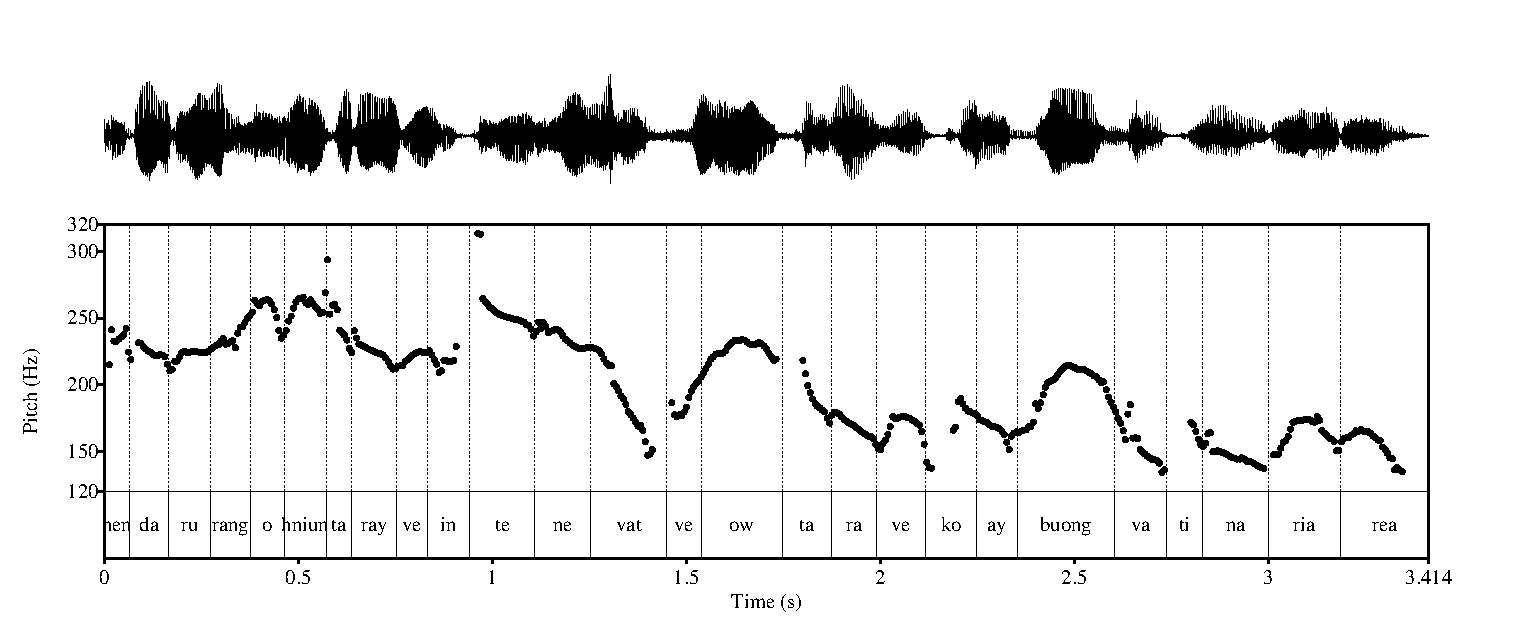
\includegraphics[width=\textwidth]{PRAAT/pearOniLATCH.eps} 
\caption{F$_0$ contour of example (\ref{Wooi_Oni})}\label{fig:Wooi_Oni}

\end{figure}
\

\pex \label{Wooi_Oni}
\a
%\begingl
%\rightcomment{{\small \textbf{Wooi} \textsc{pap}}}
\gll henda rurang o: hniuntaray ve intene vat \\
he-ra rurang o: hniuntaray ve intene vati \\
\glc 3\acs{pl}-go parallel \acs{fill} person \acs{rel} earlier \acs{det}:\acs{sg} \\
\glft `They walked alongside the man from earlier' \\ 
\z
\a
%\begingl
\gla ve owta ra ve ko aybuong vat naria rea \\ 
ve owta ra ve ko aybuong vati naria rea \\
\glc \acs{rel} climb go \acs{rel} take fruit \acs{det}:\acs{sg} again  \\
\glft `the one who climbed up who took the fruit again' \trailingcitation{{\small (WBW\_pear\_Oni)}}\\ 
\z
\xe

Furthermore, the opposite assumption is not true either. There are in fact coherent intonation contours that exhibit internal pauses. Pauses are therefore not automatically a cue for a phrase boundary: When a speaker hesitates at a certain point the f$_0$ value at cut-off may be remembered and resumed at exactly the same level after the pause. This is to be understood as a continuation and not as a phrase boundary. Consider the following example from another Wooi pear story narration. In contrast to the case in (\ref{Wooi_Oni}) above, the speaker resumes the intonation contour at almost exactly the same pitch level as it was on \textit{na} right before the hesitation pause (if one were to cut out the pause, both ends of f$_0$ would fit together quite well).

\begin{figure}

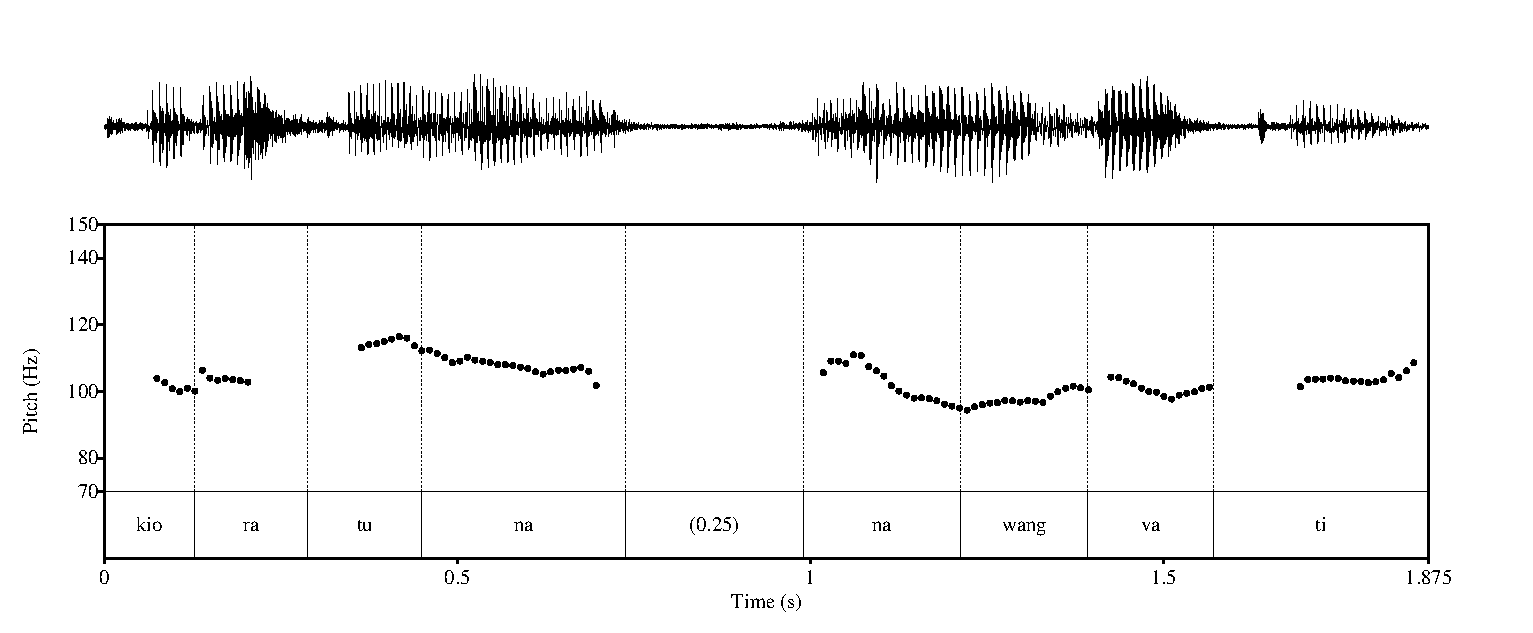
\includegraphics[width=\textwidth]{PRAAT/pearJohnHESIT.eps} 
\caption{F$_0$ contour of example (\ref{Wooi_John})}\label{fig:Wooi_John}

\end{figure}
\

\ea \label{Wooi_John}
%\begingl
%\rightcomment{{\small \textbf{Wooi} \textsc{pap}}}
\gll kio ra tu na \nogloss{(0.25)} nawang vati \\
$<$i$>$ko ra tura na nawang vati \\
\glc $<$3\acs{sg}$>$take go stand \acs{loc} basket \acs{det}:\acs{sg} \\
\glft `He took (them there and) left (them) in the basket' \trailingcitation{{\small (WBW\_pear\_John)}}\\ 
\z
\xe

So, to conclude at this point, the observation behind these arguments is that prosody seems to indirectly cue the existence of SVCs. There is certainly some sense in this argument if we look at 'minimal pairs' such as the one given by Schapper (2009) for Bunaq:

\ea \label{bunaq2}
%\begingl
%\rightcomment{{\small \textbf{Bunaq} \textsc{nus}}}
\gll Markus bola wa rebel \\
Markus ball discard descend \\
\glft `Markus threw the ball away downwards.’ or `Markus threw the ball away, (and he went) downwards.’  \trailingcitation{{\small (Schapper 2009: 442)}}\\ 
\z
\xe

Depending upon prosodic output, the example in (\ref{bunaq2}) may have two quite different readings. If uttered under a `single' intonation contour with a high boundary tone aligned to the first syllable of \textit{rebel}, the construction is interpreted such that it is the ball that descends. However, if there is a prosodic `break' between \textit{wa} and \textit{rebel}, and a final high tone is aligned to \textit{wa}, the interpretation is that it is Markus that descends after discarding the ball (thus making it two distinct event frames) (Schapper 2009: 442).

There is, however, a shortcoming with this argument. If a coherent f$_0$ always cues an SVC and an `incoherent' contour automatically precludes an SVC interpretation, then it would follow that the prosody - syntax mapping is exactly one to one. This would be a challenge for already established syntactic units such as the monoverbal clause. We know that clauses do not always neatly align with prosodic phrases (neither with \acs{IP}s nor with intermediate phrases; see on this point e.g. Chafe 1994, \cite{himmelmann2006challenges}, \cite{ladd2008intonational}, also \cite{engelhardt2010}), and, indeed, I do not think that it is an exaggeration to claim that we do not know of \emph{any} syntactic unit with a constant prosodic output. Even if, ideally, speakers attempted to match syntactic clauses with coherent prosodic units, natural speech would always remain imperfect. As every field linguist is well aware, ``the physical manifestations of psychologically relevant units are always going to be messy and inconsistent" (Chafe 1994: 58). Therefore we would expect that the prosodic chunking of SVCs is subject to variation just as it is found with other syntactic units. Seen this way, the explanatory power of the prosodic argument seems to be less strong and less reliable as is suggested by the standard reading in the literature. While there might be a partial correspondence between prosodic phrases and SVCs no exclusive argument can be based on prosodic behaviour. Yet, as this criterion is almost always used in order to determine SVCs, it has been adopted in the present study for practical considerations (see section §\ref{sec:defining} for discussion).

\subsubsection{Cognitive properties} \label{sec:cognitive}

The last parameter pertains to the cognitive background of SVC construal. It is claimed that SVCs express on the grammatical level what is on the cognitive level perceived as a single event. This claim is probably also the most controversial one and has been dismissed or called into question by many authors. What does event mean? One word of caution is in order here. There are at least two meanings of `event' in linguistics. What the typologists and descriptive linguists working on serialisation mean by `event' is quite different from what semanticists have in mind: the latter use is probably older, dating back in its modern sense at least to Zeno Vendler's verb class analysis \parencite{vendler1957verbs}. Here, event refers to a class of verbs (to the exclusion of stative and activity verbs) that can be deduced by testing their lexical aspect. Events in this sense are roughly equivalent to `dynamic verbs', or to `dynamic events' in Haspelmath's (2016) sense. 'Events' in the serialisation debate are not clearly defined but, very roughly, pertain to chunks of space and time in which something is happening (for instance, a basket of pears is stolen, or a pig is dying) and this something is perceived as having a starting point and an end point. So far so good. The trouble starts when it comes to the question of how these delimiters can be detected. Aikhenvald's definition patently demonstrates the challenge of this question:

\begin{quote}[S]emantically, serial verb constructions may encode one event, or several subevents
closely linked together, or even several subevents in sequence which may be conceptualised as
connected to each other. In the latter case, it may appear hard to draw a tight semantic distinction
between a monoclausal serial verb construction and a sequence of clauses. (Aikhenvald 2006: 12)\end{quote} 

There are several problems with this definition, both terminological and theoretical. First, we encounter two different concepts: events and sub-events. What is the relationship between events and subevents? Does every event consist of subevents, and if so, of how many\footnote{Aikhenvald speaks of "indissoluble" events which implies that there might also be events without a compositional structure (2006: 12).}? What sounds like a part-whole relation is actually not defined by theory (see also Bohnemeyer et al. 2007: 499 on this point). If we by analogy compare events with syntactic units like a VP one could wonder whether events are also projected by subcomponents, that is, whether events are hierarchical in ways similar to constituent structure in syntax or to phonological structure. Yet there has been no real attempt in the serialisation debate to address such questions. 

A further terminological problem with Aikhenvald's definition arises with the phrases `subevents closely linked together' and `subevents [...] conceptualised as connected to each other'. What exactly is the difference between subevents being linked together and subevents being (conceptually) connected? As long as such notions cannot be made operational and useful to typological approaches, nothing is gained by including such claims into definitions of a phenomenon that is in and of itself only vaguely characterisable. Obviously, what authors have in mind when they speak of subevents is plainly the lexical condensation points of human event perception and segmentation, that is, verbs. My impression is that `different subevents connected together' is often interchangeable with `different verbs connected together'. Haspelmath (2016: 15) makes a similar point in remarking that

\begin{quote}[a]s far
as I can tell, whenever a clear contrast between a single event and multiple events has
been noted, it makes the same distinction as the grammatical criteria, in particular
monoclausality and biclausality.\end{quote}

He then concludes that the event parameter is not a necessary criterion for SVC determination. While that is certainly right at this point, I want to introduce very briefly two approaches that have tackled the event concept from different angles. The question that Bohnemeyer and colleagues (2007, 2011) posed was: ``How should linguistic event segmentation be measured?" (Bohnemeyer et al. 2007). Instead of matching event boundaries with syntactic or prosodic boundaries, they took the temporal frame of event expressions as their starting point and developed the 'macro-event property' (MEP). A MEP is defined as follows:

\begin{quote}A construction has the MEP if temporal operations such as time adverbials,
temporal clauses, and tenses necessarily have scope over all subevents encoded by
the construction. (Bohnemeyer et al. 2007: 497)\end{quote}

Whether or not a given construction has the MEP can be tested by applying a temporal operator. Thus, in the following example from Bohnemeyer et al. (2007: 503f.), (\ref{bohne1}) has the MEP, but (\ref{bohne2}) does not.

\pex 
\ea
\ea
\label{bohne1} Floyd went from Rochester via Batavia to Buffalo.
\ex *Floyd went from Rochester at seven via Batavia at seven forty-five to
Buffalo at eight thirty.
\ex \label{bohne2} Floyd left Rochester, passed through Batavia, and arrived in Buffalo.
\ex Floyd left Rochester at seven, passed through Batavia at seven fortyfive,
and arrived in Buffalo at eight thirty.
\z
\z

While temporal modification of each constituent is fine with the multiclause example in (\ref{bohne2}), it does not work with the monoclausal event conceptualisation. Modifying each PP with a temporal operator sounds odd to English speakers, and signals according to Bohnemeyer et al. that the whole construction has the MEP.

Another approach to identifying event boundaries comes from neuropsychological research, methodologically established by \textcite{newtson1976perceptual}\footnote{Many thanks to Rebecca Defina for pointing that out to me.}. \textcite{zacks2007event}) and \textcite{zacks2010we} report findings from perceptual psychology and cognitive neuroscience showing that humans make use of automatic and incremental event segmentation in order to help predict what comes next and to cope with narrow information uptake (Zacks 2010). In one experiment, participants watched films of everyday activites and had to press a button whenever they felt there was an event boundary. They did this twice. One time they were asked to segment the smallest meaningful event units, and another time they were asked to segment the largest units that were meaningful to them. The results were so consistent that it was argued that they show naturally occurring perceptual processing (Zacks and Swallow 2007: 80). In other experiments, participants viewed the video clips passively the first time before they were asked to do the segmentation. The segmentation data were then compared to brain activity data. Such data seem to suggest that event segmentation is something that we humans do all the while when we actively engage with the world. However, as Zacks \& Swallow (2007: 81) noted 

\begin{quote}there is evidence
that observers can adapt their performance of the buttonpressing
segmentation task based on situational needs. For
example, observers adjust the temporal grain of their segmentation
based on explicit instructions, the sort of information they
are trying to learn from a stimulus, and how much they know
about the activity they are watching.\end{quote}

We have seen in the introductory chapter that the ``all-new approach" sets out from the assumption that SVCs are essentially different from clause linkage types, and might therefore reflect underlying differences in event perception and construal. A recent study by Defina and Majid (2012) looked into memory effects associated with the use of different grammatical constructions, raising the question whether the use of SVCs might bear on the ability of speakers to recognise and retrieve events. Speakers from English and Avatime (an African language with extensive use of serialisation) were asked to memorise short video clips of putting and taking events. Defina and Majid showed that false recognition of putting and taking events was more likely in Avatime when speakers produced SVCs in a \textit{post hoc} event description, whereas English speakers showed no difference in event recognition with regard to different grammatical constructions. Such findings may suggest that speakers of serialising languages can group event elements together, and store them as event units.

Summing up this section, although evidence from cognitive research amounts to the understanding that event segmentation is a naturally occurring human task, it is still controversial how this is actually reflected in linguistic chunking. Bohnemeyer and colleagues propose that event chunks are basically defined by their inherent temporal properties. Thus, temporal modification seems to be the most reliable test so far in order to detect the boundaries of `deeper' mental units that are different from better known linguistic units such as the clause.

\subsection{Coherence or Composition} \label{sec:coherence}

In the previous sections, I discussed cues to SVC detection that are regarded as standard arguments throughout most of the contemporary literature. In the following sections, I will introduce some further concepts that are not directly used as cues but form a more general backdrop of reasoning. The first idea to consider here is the concept of coherence. What makes a string of elements a coherent construction? All arguments introduced above as part of the `standard list of arguments' are actually based on a notion of coherence. The verbs form a coherent syntagma (the clause) on the basis of a coherent prosodic pattern, a coherent cognitive conceptualisation, as well as a coherent set of referents that is turned into `shared' grammatical arguments. All this reveals an important presupposition that is not always made explicit: that SVCs indeed constitute a unit (or construction) and do not consist of juxtaposed clauses (or VPs). This coherent unit has been addressed by features from different linguistic levels assuming that the boundaries of the phenomenon show through the different layers of the language system (for instance by prosodic chunking). This direction is in line with the ``all-new approach" that I outlined right at the beginning of the introductory chapter. The premise is that this unit is different from the traditionally recognised linguistic units (monoverbal clause, biclausal sentence). 

The presupposition of underlying coherence is, however, not prevalent in all approaches. Mostly in older contributions, we find proponents of the ``nothing-new approach" that assume that there is, though covert, an asymmetry in the verbs' ranking and that two VPs are linked together in ways similar to complementation or subordination strategies in other languages. A good example for this line of reasoning is Seuren's (1991) proposal of serialisation as an instance of pseudocomplementation. He defines pseudocomplementation as follows (Seuren 1991: 196): 

\begin{quote} A pseudocomplement is a suppositious sentential complement, foisted on a verb whose meaning requires no such complementation, and expressing concomitant circumstance, purpose, or result. Pseudocomplements are opposed to proper complements, which are semantically required by the governing verb.
\end{quote}

Thus, in essence, what Seuren has in mind is an adjunct VP\footnote{as opposed to cases of lexically governed pseudocomplementation such as in \textit{John went fishing} versus \textit{*John walked fishing} where the verb \textit{go} allows for a pseudocomplement whereas other English motion verbs do not (see Seuren 1991: 197).} tied to a matrix VP by specific grammatical rules: first, ``a controlled deletion (or non-expression) of the subject of the pseudocomplement (let's call it Secondary Subject Deletion or SSD)", and second, (optional) ``tense and/or agreement copying from the higher verb" in order to explain double-marked verb strings (Seuren 1991: 197).

The pseudocomplement approach and similar takes on verb chains aim at saving the generativist model of a single clausal head. Baker (1989) has also argued for an analysis that would leave the basic assumptions of the by-then version of government-and-binding intact. Baker proposed a system of double $\theta$-marking where both V$_1$ and V$_2$ $\theta$-mark the shared object argument of a given SVC in any SVO language. One of the outcomes of his proposal was an asymmetry in the status of V$_1$ and V$_2$ with the former verb being a structural sister to the object argument, and the latter being its structural daughter. Durie (1997) has argued convincingly against such an analysis, pointing out that Baker's approach is not consistent with the data.

Whatever the theoretical backdrop of composite approaches is, they do raise the question about what it is that makes us so sure that underspecified verb sequences really form a coherent unit, or even more specific, a construction, as the standard term serial verb construction has it. Although it appears from the contemporary literature on serialisation that the coherence side has won the day, the issue of composition will resurface in later chapters of this book, and we will ultimately see in chapter \ref{ch:discussion} that both coherence and composition do seem to play a major role in the formation of MVCs in EI.

\subsection{Construction and productivity}

In what sense, then, are SVCs constructions? In contemporary linguistic theories, there are at least two definitions of construction, a loose one and a strict one. While the loose one is used more or less as a desriptive cover term for a grammatical unit that consists of several items (lexemes and formatives), the strict one has a more narrow definition. For instance, Goldberg (1995: 4) defines a construction as follows. 

\begin{quote}Constructions are taken to be the basic units of language. Phrasal patterns are considered constructions if something about their form or meaning is not strictly predictable from the properties of their component parts or from other constructions. That is, a construction is posited in the grammar if it can be shown that its meaning and/or its form is not compositionally derived from other constructions existing in the language.\end{quote}

If SVCs are viewed this way, we would assume that the meaning of the construct contains more than just the sum of the verb meanings. In other words, understanding `construction' in its strict sense would entail the postulation of non-compositional meaning in SVCs. Reconsider the Bunaq example in (\ref{bunaq2}) from section §\ref{sec:prosodic} above. There is two verbs in sequence, indicating a downward movement of the ball away from the actor. To make it non-compositional in Goldberg's sense, the construction would need to convey a meaning that cannot be inferred from the meaning of the two verbs expressed in isolation. Indeed, as we have seen, prosody may coerce two quite different readings. The utterance could either be interpreted as a complex motion event where it is the ball that descends. This would entail a change in the alignment of syntactic function and semantic role (as the theme-object of V$_1$ becomes the actor/theme-subject of V$_2$). Or, if prosodically phrased in a different manner, one might read the sequence as consisting of two events, both performed by one and the same actor (throwing the ball, and then going). If the claim is that reading 1 is preferred under a coherent intonation pattern, then one could argue that the construction as such selects the change in alignment, and neither of the verbs would suggest so when viewed in isolation.

However, as far as I can see, the whole discussion of SVCs makes very little reference to the concept `construction', and does little to explain the consequences that the term might entail in a strict sense. Haspelmath (2016) is among the authors that explicitly refer to constructions. He puts it as follows:

\begin{quote}To fall under my definition, a serial verb construction must be a productive schematic
CONSTRUCTION such that the meaning of a concrete construct can be determined on
the basis of the meanings of its parts and the construction meaning. This means that
non-compositional combinations of verbs do not fall under the definition. (Haspelmath 2015:6, emphasis by the author) \end{quote}

Strictly speaking, ``concrete constructs" that consist not only of lexical meaning components but also of ``constructional meaning" are to be considered non-compositional according to standard definitions in literature on constructions (see for instance Goldberg 1995, 2006, Croft 2001). Understood from a constructionist point of view, Haspelmath's definition that ``non-compositional combinations of verbs" are not considered would probably leave \emph{no} SVC at all in his basket. This is in all likelihood not what he has in mind. Non-compositional in Haspelmath's sense rather seems to be equivalent to non-productive. This is, however, not exactly the same. There are both productive and unproductive SVCs in many languages but both types are non-compositional rather than compositional. Take for instance the position-action construction from Wooi (see discussion in section §\ref{sec:position-action}).

\ea \label{}
%\begingl
%\rightcomment{{\small \textbf{Wooi} \textsc{pap}}}
\glll hninyong katung mey teti tatuva wona pi \\
hninyong katung $<$i$>$mahoy $<$i$>$tati tatuva wona pi \\
 child little $<$\acs{3}\acs{sg}$>$sit $<$\acs{3}\acs{sg}$>$peek along dog \acs{det}.\acs{sg} \\
\glft 'the child sat staring at the dog' \trailingcitation{{\small (frogstory\_Kosmus)}}\\ 
\z
\xe

We find two meaning components at work: first, there is the meaning from the two verbs \textit{mahoy} 'sit' and \textit{tati} 'peek' (ignoring the postverb \textit{tatuva} for the moment). Second, there is a meaning component that directly resides in the construction: neither the semantics of the sit verb nor of the peek verb tell us that both events go on simultaneously. For Wooi speakers the reading of this construction is always that of assuming a position and doing something at the same time. Such non-compositional meaning components are most probably inherent in most if not all SVCs. So, as a consequence I would rather assume (\textit{contra} Haspelmath) that canoncial SVCs are inherently non-compositional.

Productivity is a further parameter that is often invoked. As Haspelmath put it, `good' SVCs are considered productive and schematic (which makes them different from lexicalised constructions such as Zwicky's dismissive \textit{go jump in the lake}; Zwicky 1990: 9). Productivity seems to presuppose a construction with slots into which verbs from certain semantically or functionally defined classes may enter. A construction then is productive if it would minimally allow new verbs into one of its slots. If one wanted to get rid of someone, \textit{go leap in the lake} or \textit{go jump in the bathtub} would most probably not have the same effect as \textit{go jump in the lake} precisely because there is no slot available that would allow new items. While the thought of productive SVCs seems appealing at first, we do know of many examples from the literature where authors discuss limits to productive patterns. An oft-repeated pair of examples, one licit and one illicit, is from \textcite{sebba1987syntax}:

\pex \label{}
\a
%\begingl
%\rightcomment{{\small \textbf{Sranan}}}
\gll a teki a fisi seri \\
(s)he take the fish sell \\
\glft `(S)he sold the fish' \\ 
\z
\a
%\begingl
\gla *a teki a fisi bay \\ 
(s)he take the fish buy \\
\glft intended: `(S)he bought the fish' \trailingcitation{{\small (Sebba 1987: 60)}}\\ 
\z
\xe

While taking the fish to sell it is fine, taking the fish to buy it is rejected by speakers of Sranan. Durie has referred to such limitations as `the unacceptability of non-events' (1997: 327), proposing that the latter sequence is not a proper ``stereo-typical schema" for event-types in that particular language. I do not want to call this explanation into question. Yet it seems plain that `productive' SVCs are not quite that productive and that there is a number of language-internal or crosslinguistically valid restrictions at work. Even constructions that seem to be among the most productive ones, such as the highly frequent motion-to-action construction in EI languages with a motion verb followed by an action verb, are somehow restricted. Rarely have I seen any example of a motion-to-action construction in the EI data that would not feature an action verb in V$_2$ where the action is brought about willingly and the actor is in full control of the situation. There is nothing like 'he went fell into the lake' or 'he went noticed the child' which suggests that the construction as such has a meaning component \textsc{go somewhere + do something volitionally}. This precludes a large class of verbs that come with a non-volitional or non-control reading.

Productivity is thus a problematic concept: first, it does have clear limitations as a result of which fully productive SVCs probably do not exist (see also Sebba 1987: 40). And second, no author has to my knowledge tried to make productivity operational by using some measure of quantification. Is a construction productive if it allows, say, twenty different verbs into one of its slots? Or is a construction productive if it allows all verbs of one semantic class (or field)? And if so, how can we delimit the semantic class? As long as these questions are not answered it does not make much sense to speak of productive SVCs unless we only want to emphasize that they are different from fixed lexicalised chunks. Productivity (as so many other linguistic parameters) is thus rather a matter of degree than a matter of either/or\footnote{Enfield made a related point regarding symmetrical and asymmetrical constructions, claiming that the choice between `restricted' and `unrestricted' verb slots (or rather verb classes, as some authors misleadingly claim) is rather a matter of personal intuition than of objective criteria. He writes: ``Though the distinction open versus closed is ostensibly discrete, there is much range in what is taken by different authors to fall into one or the other type, illustrated, for example, by the possibility of positing `closed classes’ with as many as 100 items (in Dumo; Ingram’s chapter, 202), or even 600 items (in Ewe; Ameka’s chapter, 125)" (Enfield 2006: 449).}.

Some authors even seem to conflate productivity with frequency. For instance, Bril (2004) in her discussion of ``frequency and productivity" of Oceanic SVCs gives a table on p. 9 that has the title ``productivity of serial constructions". Yet the values she assigns to the different constructions/languages in the table cells clearly belong to the quite distinct category of frequency (``rare", ``infrequent"). The same conflation reappears in the prose: ``In the languages of New Caledonia, serial verbs also vary from productive [...] to infrequent..." (Bril 2004: 10). While there is certainly an overall tendency of highly productive constructions to occur in high frequencies, this is not a strict correlation or entailment but rather epiphenomenal. Constructions that are frequently used are salient construals and therefore arguably tend to be made productive by high patterns of usage. And conversely, highly productive constructions are prone to be used in new contexts, which makes them all the more frequent. Yet this is not always the case. To give a simple example, directional MVCs in Wooi only feature three directional verbs in V$_2$ and a couple of motion verbs in V$_1$. Yet despite this very restricted productivity, this construction belongs to the most frequent construction types in that language. Depending on the text genre taken, frequency of occurrence can be as high as every second to third IP. In much the same vein, formulaic lexicalised SVCs with fixed content may occur in high frequencies depending on the specific communicative function. Therefore, efforts should be taken to discriminate carefully between these two variables.

\subsection{Symmetrical vs asymmetrical SVCs}

From productive SVCs and open versus closed verb slots it is only a tiny step to symmetrical and asymmetrical SVCs. It is one of the most widely used concepts in the serial verb debate that SVCs may either be symmetrical or asymmetrical whereby symmetry pertains to the relationship between the status of the verbs. The idea of symmetricity in serialisation was primarily developed by Aikhenvald (1999, 2006, though Sebba 1987 already speaks of fixed verbs and free verbs), and has since been used by many authors of descriptive studies (for EI language descriptions, see for instance Kratochvíl 2007, and Bowden 2001).

In Bril (2004: 5) we find the following delimitation: \begin{quote}Symmetrical serial constructions consist of several co-ranking nuclei which belong to an open class, none of them determining either the semantic or the syntactic property of another verb of the sequence, and all under equal scope of a negation marker.\end{quote}

The key components in this definition are: co-ranking nuclei, open class, not property-determining, and equal scope of negation marker. Asymmetrical SVCs, on the other hand, are made up of the following properties: \begin{quote}Asymmetrical constructions [...] comprise hierarchized nuclei (i.e. a head and a modifier). The head belongs to an open class, while the modifier may come from a smaller, closed class with a variety of meanings and functions (such as verbs expressing direction, motion, posture, property, cause-effect, aspect, modality, etc.).\end{quote}

What we can gather from these definitions is that we are dealing here with antagonistic feature pairs: co-ranking contrasts with hierarchized and open class with closed class (and large with small, apparently). The two other properties of symmetrical SVCs are not named in the definition on asymmetrical SVCs, but it is probably implied that they have the opposite value there: nuclei do determine the semantic or the syntactic property of another verb in asymmetric SVCs, and may show varying scope of a negation marker. In a later paper, Bril (2007) explicitly stated that co-ranking is meant to be equivalent to ``coordinate constructions" while hierarchised is used for ``subordinate constructions", but this does not seem to be very elucidative either\footnote{In fact, it is not clear whether coordinate and subordinate in Bril's sense pertains to coordination and subordination of clauses or to something else. If to the former, one would end up with the confusing notion of clause combinations taking place within single clauses.}.

The terms 'co-ranking' and 'hierarchised' seem more or less equivalent to '(grammatical) status' in other work. Aikhenvald (2006: 22) gives the following definition of symmetrical serial verbs:

\begin{quote}Symmetrical serial constructions are not 'headed' in the way asymmetrical ones are: all their components have equal status in that none of them determines the semantic or syntactic poperties of the construction as a whole.\end{quote}

While this sounds quite similar to what Bril defined (see above), there is an interesting difference: being on the same rank in Bril's understanding means that none of the verbs exerts semantic or syntactic influence on the respective other verb. In Aikhenvald's definition, being on the same rank means that none of the verbs determines the semantic or syntactic properties of the construction. Asymmetrical SVCs, on the other hand, 

\begin{quote}denote a single event described by the verb from a non-restricted class. The verb from a closed class provides a modificational specification: it is often a motion or posture verb expressing direction, or imparting a tense-aspect meaning to the whole construction.\end{quote}

This is then illustrated by an example from Cantonese in which a \textsc{take} verb combines with a motion verb whereby the latter ``provides directional specification to the SVC" (Aikhenvald 2006: 22).

\ea \label{}
%\begingl
%\rightcomment{{\small \textbf{Cantonese}}}
\gll lei$^5$ lo$^2$ di$^1$ saam$^1$ lai$^4$ \\
you take \acs{pl} clothing come \\
\glft `Bring some clothes' \trailingcitation{{\small (Aikhenvald 2006: 21)}}\\ 
\z
\xe

What is problematic with the symmetrical-asymmetrical approach, however, is that authors seem to deviate from each other when assigning SVCs to either group. A puzzling example is provided by Kratochvíl (2007) who presents the following construction as an example for a symmetrical SVC:

\ea \label{}
%\begingl
%\rightcomment{{\small \textbf{Abui} \textsc{nus}}}
\gll mi me feng \\
 take come injure \\
\glft 'bring to slaughter' \trailingcitation{{\small (Kratochvíl 2007:351)}}\\ 
\z
\xe

The sequence is made up of three verbs, a \textsc{take} verb, a motion verb and an action verb: presumably, the actor obtains some object and moves to some place suited for the final action to be carried out. Or does he/she have something in his/her possession \textit{while} moving to the place of slaughter? The first part of the construction looks just like the Cantonese example from Aikhenvald above, and it just receives the same translation, rendered into English by a monoverbal structure `bring'. While Aikhenvald considers \textsc{take} plus motion to be an asymmetrical construction, Kratochvíl describes it as being symmetrical (2007: 351):

\begin{quote}These verbs are of equal grammatical status; they do not show any dependency with respect to each other. This means that none of the verbs [...] is semantically `dominant'.\end{quote}

Two conclusions could be drawn from this disparity. Either roughly homologous constructions belong to different symmetricity classes in different languages, that is, while \textsc{take} plus motion is asymmetrical in Cantonese, the Abui construction belongs to the class of symmetrical constructions. This would come as a surprise, however, given that the English translations in both cases seem identical. Alternatively, we might conclude that the symmetricity criterion is as of yet not defined well enough to allow for crosslinguistic application. 

\subsection{Nuclear vs core-layer SVCs}\label{sec:nuclear}

Work on verb serialisation has quite often made use of the `layered structure of the clause'-model from RRG (Olson 1981, Foley and Van Valin 1984, Van Valin and LaPolla 1997). The clausal architecture in RRG is different from other approaches to constituent structure in that the clause is not analysed as a projection from the finiteness features of the main verb. Instead, three layers are assumed to be active in clause structure, each one having its own constituents and its own operators: the nucleus is the innermost layer, and basically consists of the verb(s) and further formatives together constituting the predicate\footnote{Note that predicate in this sense does not include any of the verbs arguments. The nucleus in Foley and Van Valin's design may also comprise more than one predicate allowing for multipredicate clauses (a view that is in conflict with most definitions of serial verbs that assume one (complex) predicate within what is considered one clause; see Foley and Van Valin 1984: 77).}. The next layer is the core where the arguments of the verb(s) are placed (hence `core arguments'). Around the core, the outermost layer called periphery subsumes non-core arguments (adjuncts, oblique arguments) and secondary participants in the event (Foley and Van Valin 1984: 77). This layered structure of the clause is claimed to be universally present in languages, and in comparison to immediate constituent-approaches the theory also draws on evidence from non-configurational languages (Foley and Van Valin 1984: 78).

What makes the layered structure of the clause so appealing to authors working on serialisation is that it provides a straightforward explanation for different argument verb patterns in these languages. Any layer is able to combine with another building block of the same type, that is, allowing combinations of nuclei, cores or peripheries. Foley \& Van Valin (1984: 188) refer to these combinations as junctures. They write:

\begin{quote}A nuclear juncture is a construction with a complex nucleus. It is a single unit, and all core and peripheral arguments are arguments of this complex nuclear element. In core-level junctures two cores, each with its own nucleus and core arguments, are joined together to form a larger complex core. The peripheral arguments must be shared by both cores, as they form a single complex unit within the peripheral layer. Peripheral junctures involve the joining of two clauses with independent peripheries.\end{quote}

In nuclear-layer juncture and in core-layer juncture, the periphery is shared by both juncts and so the whole construction still forms just one clause. As there is further variation with regard to the status of the arguments (in nuclear-layer juncture all core-arguments are arguments of the complex nucleus while in core-layer juncture, each verb (nucleus) governs its own core arguments) two different types of serialisation structures have been mapped on this model: in nuclear-layer serialisation, two verbs stand in direct sequence (contiguous) surrounded by the core arguments (which are arguments of the complex nucleus, as defined above). In contrast, core-layer serialisation has two verbs in non-adjacent position where the arguments of each verb may be placed between them (either the object of the first verb, or the subject of the second verb). The following table from Bril (2004) gives a structural overview of both types.

\begin{table}


\begin{tabular}{ll}
\hline \textbf{Nuclear-layer serialization} & \textbf{Core-layer serialization} \\
\hline 
\pbox[c]{0.5\textwidth}{\textbf{sVV(o)} \\
 I run catch (him) } & 
 \pbox[c]{0.5\textwidth}{ a) same-subject: \\ \textbf{sVsV(o)} \\
 I run I catch (him) \\  \\
 b) switch-subject: \\ \textbf{sVo(s)V} \\ 
 (o = s) I strike him (he) dies }  \\
\hline
one single set of arguments & verbs share at least one inner argument \\
\hline
\end{tabular}
\caption[Nuclear and core-layer serialization]{Nuclear and core-layer serialization, taken from Bril (2004: 4).}


\end{table}
\

Two points seem crucial here. First, the surface structure differs with regard to the feature `contiguity'. A second difference pertains to the relation between arguments and verbs: in nuclear-layer serialisation both arguments are selected by the nucleus complex (if transitive). In core-layer serialisation, each verb selects the same actor argument (same-subject type) or the U argument of the first verb is selected as A by the second verb (switch-subject type). Consider the following example from Olson's (1981) foundational discussion of Barai (Papuan):

\pex 
\a \label{barai1}
%\begingl
%\rightcomment{{\small \textbf{Barai}}}
\gll fu fi fase isoe \\
\acs{3}\acs{sg} sit letter write \\
\glft `He sat down and wrote a letter' \\ 
\z
\a \label{barai2}
%\begingl
\gla fu fase fi isoe \\ 
\acs{3}\acs{sg} letter sit write \\
\glft `He sat writing a letter' \trailingcitation{{\small (Foley and Van Valin 1984: 190)}}\\ 
\z
\xe

In (\ref{barai1}), the two verbs \textit{fi} 'sit' and \textit{isoe} 'write' combine in a core-layer serialisation, the U argument of the second verb separates both verbs. In (\ref{barai2}), the same verbs are placed adjacent to each other and the arguments precede the nucleus complex hence we deal with nuclear-layer serialisation. Both constructions differ nicely with regard to their semantics, further motivating the claimed constructional difference.

\subsection{Further variables}

The last sections have addressed variables with quite different status. While coherence and productivity are claimed to be a property of all SVCs by most authors, symmetricity and the varying juncture levels have been discussed as internal variables, corresponding to different subtypes of SVCs. As we have seen in the preceding section, nuclear- and core-layer serialisation draws on a number of variables at a finer grain: contiguity is needed in order to detect nuclear-layer serialisation (no argument may intervene between the verbs). Another variable that is at least indirectly tied to Foley \& Van Valin's dichotomy of junct relations in SVCs is wordhood. In languages where serialised structures consist of verb roots within one phonological word, the arguments are typically placed outside the word. What follows from this is that single-word SVCs are necessarily also nuclear-layer constructions. 

Wordhood is not an uncontroversial property. Some authors exclude serialisation on the root level because they assume that compounding is a different process and belongs to a different linguistic tier. For instance, Van Staden \& Reesink (2008: 27) argue very carefully for a distinction between verbal compounding and what they call complex serialisation. Others like Aikhenvald treat wordhood as an internal variable, stating that ``components of a serial verb construction may or may not form independent grammatical or phonological words" (2006: 3).

Another variable that I have mentioned already is variation in the marking of the verbs. While hardly any language seems to allow for free variation in verb inflection patterns\footnote{Tidore, a Papuan language of Halmahera, which is included in the EI dataset, appears to represent the odd one out. Subject indexing inflection can be added to verbs or left out in what seems to be free variation (see van Staden 2000).}, many languages employ different strategies in different constructions. If one does not exclude cases with differential marking altogether (by arguing that differences in inflectional status entail hierarchical differences within the construction), at least two distinct values are possible here: constructions where all verbs are treated alike, and constructions where we find differences between the verbs. As we have seen in  chapter \ref{ch:area}, many EI languages show irregular or unstable inflection patterns that are phonologically or lexically conditioned. Other languages do not even have verbal inflection systems. These are clear obstacles to applying this variable crosslinguistically.

Before closing this section, I would like to mention briefly another language compartment that is associated with the communication of event expressions. Recent work on gestures has suggested that co-speech gestures might be a useful tool for the detection of SVC boundaries. Defina (2016) showed for Avatime (Niger-Kongo) that while single gestures tend to overlap the whole SVC, clause-linking constructions are more likely to be associated with more than one gesture, overlapping single verb phrases rather than the entire construction. Such evidence will certainly make a valuable contribution to our understanding of serialisation, and might even help overcome the single event conundrum.

\section{Previous work on SVCs in Australasia} \label{previouswork}

The preceding sections have reviewed a set of criteria or variables that have been introduced in order to argue for external limits to and internal variation within the serialisation category. As I have tried to show, many of the variables are as of yet not operational in the sense that there are well-defined threshold values that researchers have agreed upon. Despite the ongoing debate on many of these variables, there has been considerable research into languages in EI as well as into neighbouring areas. 

In the following sections of this chapter, I will have a look at this research and approach the question how these variables have been put to use for language families in and around Eastern Indonesia. I will first discuss the results of Bril's research into Oceanic languages, then review van Staden \& Reesink's work on Eastern Indonesian languages, and finally introduce Pawley's analysis of Kalam, one of the most remarkable serial languages. All three approaches have in common that they propose new ways of ordering SVCs into classes. Bril has argued for a discrimination between co-ranked and hierarchized constructions, van Staden \& Reesink have advocated a hybrid classification into four types (independent, dependent, co-dependent and complex serialisation), and Pawley has differentiated between compact and narrative serialisation in Kalam. These sections therefore not only serve as a short introduction into studies from Australasia, but aim at discussing the potential applicability of the proposed types.

\subsection{Bril: Co-ranked vs hierarchized}

Research into serialisation in Oceanic languages has produced a good number of publications (for instance, \cite{durie1988verb}, \cite{bradshaw1993subject}, \cite{crowley1987serial}, 2002). Bril contributed to this research with her papers on \textit{Complex nuclei in Oceanic languages: Contribution to an areal typology} (2004) and \textit{Nexus and Juncture Types of Complex Predicates in Oceanic Languages} (2007). Drawing on a number of variables from other authors (like Foley and Van Valin's distinction into nuclear- and core-layer constructions), she developed a further subdivision into co-ranking versus hierarchized SVCs. 

Bril defines co-ranking constructions in Oceanic languages as follows:

\begin{quote}Co-ranking predicates belong to an open class; none of them determines the
semantic or syntactic property of another predicate of the sequence. They generally
refer to sequential actions done by the same agent as well as action-goal. (2007: 269)\end{quote}

This definition touches upon some of the notions from the preceding sections: Predicates (or verbs) belong to an open class, implying a symmetrical relationship in this sense (which is also expressed via the term `co-ranking'); and there is no mutual dependency between the predicated (verbs). These features are in contrast to the second category, hierarchized SVCs:

\begin{quote}Hierarchized predicates comprise a main verb (the head) and a modifying verb
that do not obligatorily share the same subject [...]. The scope of the modifying
predicate is either on the main verb or on one of the arguments of the main verb (in the
depictive type). (2007: 270)\end{quote}

These two types are not specified with regard to inflection patterns, adjacency configurations or operator scope. While the latter is assumed to be shared by all verbs, adjacency (or contiguity) of constituents is part of the juncture type distinction into nuclear-layer vs. core-layer on a higher level, that is, both nuclear-layer and core-layer constructions could be co-ranked or hierarchized.

Assuming that these two types are crosslinguistically extant constructions in the Oceanic languages, Bril admits that a discrimination between co-ranking and hierarchising is not always straightforward. If activity verbs are serialised, contextual factors are needed in order to disambiguate the intended reading. For instance, the combination of a motion verb and a verb of searching could in principle receive two different readings. Consider the following example from Pileni which may either translate as `paddle in (order to) search (at some place)' or `paddle searchingly' (Bril 2007: 271):

\ea \label{}
%\begingl
%\rightcomment{{\small \textbf{Pileni}}}
\gll Na no ua hehega na ko matu tuohine na \\
\acs{3}\acs{sg} \acs{ta} paddle search \acs{dem} \acs{top} \acs{1}\acs{pl}.\acs{ex}.\acs{poss} sister \acs{dem} \\
\glft `He has paddled here in search of our sister.’ \trailingcitation{{\small (Bril 2007: 271, quoted from N{\ae}ss 2004: 233)}}\\ 
\z
\xe

On the other hand, whenever a stative verb takes part in a SVC, it forms a hierarchized construction together with a main verb. This also follows from the assumption that the modifying verb has scope over the other verb or over one of its arguments. Stative verbs have a somewhat special status in the serialisation debate. While for instance Haspelmath (2016) opts to exclude stative verbs altogether, other authors tend to include them but often treat them as part of a special class (for example as minor verbs in asymmetrical serial constructions, or as ambient serialisation with concomitant predicate-argument configurations (see also the discussion in chapter \ref{ch:gram})). 

In the Oceanic languages, there are three morphological operations that derive serialised stative verbs. These are: (i) transitive concord, (ii) causative or adverbial derivation, and (iii) reduplication. This makes the Oceanic languages different from most other serialising languages with underived insertion of stative verbs. In all three operations the stative verb takes a morphological marking that is not semantically tied to its lexical meaning but to the construction as such and functions as a constructional flag rather than a `real' semantic derivation of the stative verb. As Bril put it, ``[t]his derivation does not create a lexical class of adverbs, but marks the modifying/adverbial function of the stative V2" (Bril 2007: 273). Here are some examples from different languages:

\ea \label{pileni}
%\begingl
%\rightcomment{{\small \textbf{Pileni}}}
\gll Kolu-no maoli la khoulua kip-ina themu-ina \\
\acs{2}\acs{du}-\acs{ta} true \acs{dem} \acs{2}\acs{du} keep-\acs{tr} quiet-\acs{tr} \\
\glft `If you are telling the truth, keep it quiet.’ \trailingcitation{{\small (Bril 2007: 272, quoted from Næss 2004: 236)}}\\ 
\z
\xe

\ea \label{hoava}
%\begingl
%\rightcomment{{\small \textbf{Hoava}}}
\gll Koni ome va-leani-a goe \\
\acs{fut} see \acs{caus}-good.\acs{tr}-\acs{3}\acs{sg} \acs{2}\acs{sg} \\
\glft `You will see it well.’ \trailingcitation{{\small (Bril 2007: 273, quoted from Davis 2003: 162)}}\\ 
\z
\xe

\ea \label{saliba}
%\begingl
%\rightcomment{{\small \textbf{Saliba}}}
\gll Ku-hedede-nogo-nogowai! \\
\acs{2}\acs{sg}-tell-\acs{red}-slow \\
\glft `Speak slowly!’ \trailingcitation{{\small (Bril 2007: 275, quoted from Margetts 1999: 135)}}\\ 
\z
\xe

In the first example from Pileni in (\ref{pileni}), the second verb \textit{themu} receives the same transitive marking as the first verb \textit{kip}. It seems clear that the stative semantics of \textit{themu} is not modified into anything like `you quiet it' in a transitive sense. Rather, what happens is that the construction seems to impose on the stative verb the restriction to appear with the same transitivizer suffix as the first verb. Bril refers to this process as transitive concord and stresses that transitivised stative verbs only ever appear in SVCs but never occur on their own.

In the next example from Hoava, a similar effect is achieved by modifying the stative verb with what looks formally like a causative prefix in that language. Here as well, Bril emphasizes that the causative prefix does not target the meaning of the stative verb \textit{leani} `good', that is, the reading would not be `You see (you) cause it to be good' but rather `You see it well'.

The last example from Saliba illustrates the third operation. Here, the stative verb is reduplicated in V$_2$, a structure that looks much like adverb derivation in other languages. Bril again notes that ``[i]t is not a lexical but a derivational device marking the modifying function of the V2 and its syntactically dependent status" (2007: 273). The difference between this and adverb deriving operations, such as the addition of \textit{-ly} in English, seems slight indeed, and rests upon the assumption that `slow' in Saliba is a verb and not an adjective.

Bril's dichotomy into co-ranked and hierarchized constructions is most clearly applicable in cases with stative verbs showing transitive concord. Concord of this kind may be marked by formatives derived from or related to causative affixes, transitivizers, or reduplication. While all these morphological devices are also in use in various languages of EI, I have not found any structural correlation of 'transitive concord'. Given that these clear-cut cases are seemingly absent, Bril's distinction into co-ranked and hierarchized constructions would produce a high number of ambiguous constructions in EI (in the same way as Bril discussed ambiguous combinations of activity verbs). Therefore, in order to capture Bril's intuition that there is a distinction between what may be called juxtaposition and modification further operational criteria would need to be found. In the next section, I turn to Miriam van Staden and Ger Reesink's approach to classifying SVCs. As we will see, their concept is quite different from Bril's and comes without explicitly dealing with modifying relations in Bril's sense.

\subsection[Van Staden/Reesink: Independent, dependent, ...]{Van Staden/Reesink: Independent, dependent, co-dependent, complex%
\subsectionmark{Van Staden/Reesink: Independent, dependent, ...}}
\subsectionmark{Van Staden/Reesink: Independent, dependent, ...}

In their study \textit{Serial verb constructions in a linguistic area}, van Staden and Reesink (2008) investigated a sample of twelve serialising languages from Eastern Indonesia (six Austronesian languages and six Papuan languages) in order to explore potential genealogical and areal relationships. Their study covered much of the area that is also investigated in the present work, with the major exception of Sulawesi. Nine of the languages that van Staden and Reesink took as a sample are also part of my data corpus and reappear in this study. 

Adopting a rather inclusive definition of serial verb constructions, the authors counted all instances in which ``two or more verbs occur in a single clause and none of the verbs is apparently formally subordinated to the other" (2008: 22). The potential ambiguity between serial verbs on the one hand and auxiliaries and prepositions on the other hand were ignored. However, cases of verbal compounding were excluded on the basis of prosodic evidence. 

The remaining cases are argued to fall into the following four classes: (i) independent serialisation, (ii) dependent serialisation, (iii) co-dependent serialisation, and (iv) complex serialisation.\footnote{The authors discuss another distinction into two broad types of SVCs, namely, component and narrative SVCs. The main defining feature of the former is Bohnemeyer et al.'s `macro-event property'. As this has been already discussed in the previous section, and because the exact discrimination between the two types is not entirely clear to me, I will not discuss this distinction here. Note that it does resemble Pawley's compact vs. narrative SVC approach (see next section).} While all four types are distinguished by their morphosyntactic structure, the classification is somewhat hybrid as the third type (co-dependent serialisation), as we will see, may either occur in an independent configuration or as an instance of dependent serialisation.

Independent serialisation describes the prototypical case where all verbs are equipped with the same inflectional morphology, and thus resemble an asyndetic coordinating structure. That independent serialisation is indeed not an instance of asyndetic coordination is established by language-specific properties. The authors suggest:

\begin{quote}For one language, this may be the scope of negation or placement of negation particles, for another it may be the radical change in meaning when a conjunction is inserted, or a characteristic prosodic contour. (van Staden and Reesink 2008: 23)\end{quote}

Such an approach is in stark contrast to the typological claim made for instance by Haspelmath (2016) that SVC identification must be based upon criteria that can be put to the test by applying the same operation across all languages. For van Staden and Reesink, it seems to suffice to draw on, say, prosodic evidence in one language, and on operator scope in another. The advantage of being liberal in the general definition of what to count as a serial verb is thus minimized by allowing for all kinds of further properties on the individual level of the language in question. A further problem arises with isolating languages where no choice of constructional inflection patterns can be made (van Staden and Reesink 2008: 23).

Dependent serialisation covers those constructions in which one of the verbs carries all verbal inflection, and the other appears in its bare or stripped-down form. As the bare verb does not have finiteness features, this type thus formally resembles subordinate structures or auxiliary constructions (2008: 24). Subordinate or auxiliary interpretations are ruled out in cases where there is no clear evidence in favour of such an analysis. The following example from Hatam has two dependent serialisation constructions, both of which show asymmetrical inflection patterns across the verbs (for instance, \textit{kwei} takes inflection but not \textit{buwak}).

\ea \label{}
%\begingl[glhangstyle=none]
%\rightcomment{{\small \textbf{Hatam} \textsc{pap}}}
\gll \textbf{di-kwei} \textbf{buwak} di-sutbatnya i-bou poi bu ba + i-bit da ba \textbf{n-ug} \textbf{ngat} ei bigbehei \\
\acs{1}\acs{sg}-come gather \acs{1}\acs{sg}-friends \acs{3}\acs{pl}-head few again and \acs{3}\acs{pl}-follow \acs{1}\acs{sg} and \acs{1}\acs{pl}.\acs{ex}-go see \acs{loc} forest \\
\glft `I came (and) got a few of my friends together again and they'd follow me and we'd go look in the forest (for game).' \trailingcitation{{\small (van Staden and Reesink 2008: 24)}}\\ 
\z
\xe

Co-dependent serialisation, as I have already indicated, crosscuts the previous distinction into fully-inflected vs. partially inflected SVCs. Here, it is not the inflection pattern but the argument configuration that is the defining criterion. Co-dependent serialising constructions invariably share one argument and each verb makes use of this argument in a different syntactic function: this pivot argument is the object of V$_1$ and the subject of V$_2$ (corresponding to the switch-function or switch-subject type in Aikhenvald 2006 and elsewhere). While this type seems most often restricted to causative or cause-result semantics (the object denoting the patient or theme which then is reanalysed as the subject of an unaccusative verb to specify the result of the action, the \textit{x hit y (y) die} type), van Staden and Reesink also note other uses of co-dependent serialisation patterns. For example, they cite cases from Moi where the construction seems to be in use in directional and in instrument constructions.\footnote{The examples given for Moi seem strikingly ambiguous between a switch-subject reading and an ambient reading where the subject of the second verb is not the object of the first one but in fact the whole predicate. Looking at the example of instrument use,

\ea \label{}
%\begingl
%\rightcomment{{\footnotesize \textbf{Moi}}}
\gll w-aala ton p-ai sin-keelik \\
\acs{3}\acs{sg}.\acs{m}-cut first \acs{3}\acs{sg}.\acs{nhum}-'with' knife-machete \\
\glft `First, he cut it with a machete' \trailingcitation{{\footnotesize (van Staden and Reesink 2008: 26, quoted from Menick 1996: 51)}}\\ 
\z
\xe

one could wonder if at all there is a reading available in which the subject indexer on the second verb takes up the (covert) object. This would have to yield something like `he cut it$_i$, (it$_i$) was with a machete', thus resembling a comitative argument status of \textit{sin-keelik} rather than an instrument one.}

Complex serialisation is the last SVC class in van Staden and Reesink's framework and refers to cases where two or more verbs share one set of affixes (the prefix attaching to the first verb and the suffix to the last one). In this sense, the definition corresponds to the surface structure of Foley and Van Valin's (1984) nuclear-layer serialisation (van Staden and Reesink 2008: 26). Example (\ref{ambon}) from Ambon Malay illustrates the difference between a co-dependent construction and a complex SVC.

\pex \label{ambon}
\a \label{ambon1}
%\begingl
%\rightcomment{{\small \textbf{Ambon Malay}}}
\gll be pukol anjing mati \\
I hit dog die \\
\glft `I killed dog (by hitting)' \\ 
\z
\a \label{ambon2}
%\begingl
\gla be pukol mati anjing \\ 
I hit die dog \\
\glft `I killed dog (by hitting)' \trailingcitation{{\small (van Staden and Reesink 2008: 41, quoted from Tjia 1997: 56 )}}\\ 
\z
\xe

Both constructions are reported to differ in the focus that is on the constituents. In (\ref{ambon1}) the emphasis is on the result (\textit{anjing mati}), while in (\ref{ambon2}), the focus shifts to the ``manner in which the state change is brought about" (van Staden and Reesink 2008: 41), that is, \textit{pukol mati}. While from a structural viewpoint two different constructions may be identified, the focus difference may as well reflect a more general trait of Ambon Malay, pertaining to the focus potential of different post-verbal positions (for instance, the first case could be analysed as having a filled clause-final focus slot, highlighting the resultant state, while the second configuration would feature an `incorporated' second verb as part of the main predicate). The question remains whether this information structural difference would only occur in SVCs or reappear in other construction types as well.

Now, if we look at these four types, it becomes obvious that we are not just dealing with one variable but with at least three: (i) inflectability of the verbs distinguishes independent from dependent serialisation; (ii) the functional switch in the pivotal argument is associated with co-dependent serialisation but may in fact occur with all three types (for instance as complex serialisation in (\ref{ambon2})); (iii) adjacency of verbs is a prerequisite for the affix sharing complex serialisation. Adjacency is not relevant, however, to any of the other three types, nor is inflectability relevant to co-dependent and complex serialisation though in the latter case the inflection pattern does play a role. Thus, in independent serialisation only inflectability has to have a specific value (all verbs inflected), while the other two variables may occur either way. The same is true for dependent serialisation. Co-dependent serialisation is orthogonal to the other three types as the switch-function value is optional for all types but for co-dependent serialisation. Complex serialisation can also be viewed as orthogonal if (verbal) adjacency is the defining variable. 

Concluding, it would seem more beneficial to deconstruct these four types into their key defining variables and annotate each case of SVC for all variables instead of dealing with the wealth of SVCs by means of orthogonal non-atomic feature configurations. 

\subsection{Pawley: Compact vs narrative}

The last approach to SVC classification to be discussed in this context is Pawley's and Lane's work on the Papuan language Kalam spoken in the Western Highlands Province of Papua New Guinea (Pawley 1987, 1991, 2008, 2011, Lane 2008). Kalam is a language with many peculiar features, some of which have profoundly stimulated the debate on verb serialisation. Perhaps the most striking feature of Kalam is the organisation of the verbal lexicon. Quite unlike most languages of the world, Kalam has a rather small and closed class of verb stems comprising only about 130 members (Lane 2008: 7). At the same time, a small portion of these verbs appear to have very broad and generic meanings, and these `generic' verbs contribute the bulk of verb tokens found in natural data (fifteen of these verbs account for 89\% of all verb tokens, and 35 of these generic verbs make up 98.6\%; Lane 2008: 7). This scarcity of verb stems is obviously associated with a high frequency of varying types of serialisation patterns in Kalam. While most SVCs contain two or three verbs, the practical limit to verb concatenations seems to be at nine to ten verbs (Pawley 2008: 172). The wealth and complexity of serial verbs in Kalam thus by far exceeds most other serialising languages, as the following example illustrates.

\ea \label{kalam1}
%\begingl
%\rightcomment{{\small \textbf{Kalam}}}
\gll mj bep tk d ap nb okyang jok-l ... \\
leaf plant pick get come place below throw-\acs{ss}.\textsc{prior} \\
\glft `having picked, brought back, and tipped \textit{bep} leaves down (in an oven pit)' \trailingcitation{{\small (Pawley 2008: 173)}}\\ 
\z
\xe

Some further features of the Kalam verb systems are markedly different from most verb systems in Eastern Indonesia. First, apart from the small size of the vebal lexicon, Kalam makes use of clause-chaining (marking subject (dis)continuity by subject reference marking) with medial verbs heading all non-paragraph final (coordinate-dependent) clauses (for instance \textit{jok-l} in example (\ref{kalam1}). Thus, there are at least two multi-verb operations in Kalam, operating on different levels, that is, serisalisation and clause-chaining. Second, the inflected verb in both serialised verb sequences and clause-chaining constructions always comes last. Third, there is a class of uninflectible `verbal adjuncts'. These adjuncts may form a complex predicate with a full verb and behave like an adverb, yet their meaning is often similar to that of a full-flegded verb, and sometimes the adjunct may alter the argument configuration of the complex predicate (as opposed to adverbs; Pawley 2008: 177).

By classifying Kalam verb combinations into types, Pawley found that many verbs occur together in certain grammatically and semantically definable ways. These combinations usually comprise only two or three verbs and form a `compact' construction. 

\begin{quote}A compact SVC expresses a sequence of conceptual events that are tightly integrated, grammatically and semantically. Compact SVCs are strictly V-serialising, i.e. no other morphemic material can occur between the verb roots. The verbs in the SVC share a single argument structure and the scope of negation and modifiers is always over the whole SVC. Some, perhaps most compact SVCs cannot be readily paraphrased by a multi-clause construction. Many, though by no means all are translatable by a simple or phrasal verb in English. (Pawley 2008: 172f.)\end{quote}

This definition bears resemblance to Van Staden \& Reesink's complex serialisation: the verbs are placed adjacent to each other, projecting a single argument structure. Though Kalam has its finite verb at the end of verb sequences, compact SVCs do not necessarily possess a `reversed' dependent pattern sensu Van Staden \& Reesink. This is because several compact SVCs can be combined to form what Pawley calls a narrative SVC, a larger serialised unit composed out of `nuclear' compact SVCs. In these larger concatenations only the final compact SVC bears inflection.

\begin{quote}Narrative SVCs provide a means for packing episodic reports into a single clause structure without omitting mention of any of the component events that Kalam discourse structure rules require of minimal well-formed event reports. Narrative SVCs can readily be paraphrased by multi-clause or multi-sentence constructions, where each clause specifies a distinct stage in the narrative action. Some narrative SVCs superficially resemble compact SVCs in that all the verb roots occur contiguously, without any intervening material. However, in syntactic terms narrative SVCs can be classed as VP-serialising. A clause of this class can be divided into two or more phrases each of which has a limited degree of grammatical independence. (Pawley 2008: 174)\end{quote}

Compact and narrative SVCs are thus not on a par but constitute serialisation techniques on different syntactic levels. This approach enables a hierarchical analysis of SVC levels. Pawley gives the following example:

\pex \label{}
\a
%\begingl [glhangstyle=none]
%\rightcomment{{\small \textbf{Kalam}}}
\gll basd skop am kmn pak + d ap ad \textipa{\~n}b-algb-al ... \\
g'father distant go animal kill get come cook eat-\acs{pst}.\acs{hab}.\acs{3}\acs{pl} \\
\glft `Our distant ancestors ... used to go, kill, bring back, cook and eat game mammals, ...' \trailingcitation{{\small (Pawley 2008: 171)}}\\ 
\z
\a 
$[[$go$]_{\textsc{vp}}$ $[[$game.mammal kill$]_{\textsc{vp}}$ $[$get come$]_{\textsc{vp}}$ $[$cook eat$]_{\textsc{vp}}$ $]_{\textsc{vp}}$ $]_{\textsc{vp}}$
\xe

The construction consists of two levels: a matrix narrative construction with two slots, a motion slot and another slot for the action. This action can be episodic in the sense that more than one event pattern is given in sequence. In this example, the second slot is filled by three `coordinate' compact SVCs: killing game mammals, bringing the game back home, and processing and eating it at home. Note that the three compact SVCs each have a different spatiotemporal frame: the killing is done in the woods, the bringing back connects the woods with the hunters' homes in the village, and the cooking and eating takes place in the village. Though Kalam is probably quite unique in adjoining so many compact SVCs, the multi-verb components (transport motion, cooking and eating, and, on the matrix level, motion-to-action) are all well-known also from the EI area, and the EI data set provides many examples of similar combinations (see chapter \ref{ch:constructions}). Thus it seems likely that the building blocks that Pawley identifies for Kalam are at least in parts also existant in languages of EI. This in turn suggests that the process of forming these types, mediated by culture-specific experiencing of the surrounding world and shaped by frequency-based conventionalization (and perhaps, to a certain extent, lexicalization), is part of a more general pattern of event conceptualization, in the area of Eastern Indonesia and perhaps well beyond.

\section{Multi-verb constructions} \label{section:multi-verbconstructions}

The previous sections have dealt with serialisation as a theoretical concept, and the various ways authors have approached and defined the phenomenon. In section §\ref{section:properties}, I have focused on a set of components that are central to the most widely discussed definitions of serial verbs. As I have suggested, there are two types of parameters: independent parameters that can be assessed directly by applying some testing procedure, and dependent parameters that require the definition of yet another concept. Monoclausality is a good case in point. In languages like Kalam with specific clause-final verb morphology, clausehood may be accurately determined, but in many languages of EI, verbal inflection is absent or conditioned by phonological or lexical factors. In such languages, clausehood seems to be a concept that resists an easy definition. In section §\ref{previouswork}, I reviewed three approaches to serialisation in the Australasian region. While all three approaches came up with new ways of classifying SVCs, their classificatory systems either rely on specific areal or language-specific features (Bril's co-ranked vs. hierarchized approach for instance worked best with transitive concord in SVCs with stative verbs), or on hybrid systems (as with van Staden and Reesink's four-way distinction).

The preceding discussion has shown that authors still struggle with finding the right set of delimiting criteria. What seems to work best for one language, turns out to be not applicable or even unwanted in another. It appears that the quest for watertight cross-linguistic definitions has led authors to include more and more pieces of evidence from different linguistic subsystems (think of prosody, or cognitive event construals). This profusion of criteria is only in rare cases fully applicable to a given language, and it is now more and more apparent that serialisation as a theoretical concept is far too laden with features that are hard to put to the test, while at the same time the phenomenon, as a whole, continues to have fuzzy boundaries. 

There are at least two reactions to this situation in contemporary literature on serialisation. The first reaction is to try and narrow down the inventory of defining features, sorting out those ones that are not operational (impractical in Haspelmath's (2016) terms) and thus hamper progress in cross-linguistic comparison. I have already reviewed Haspelmath's take on serialisation who claims to provide a definition that is ``considerably narrower than definitions used by most other authors" (2016: 6). 

The other reaction is to avoid the concept altogether, and instead come up with a more neutral term. The alternative that has come to be used most widely in recent years, and that I will adopt in the following chapters, is `multi-verb constructions' (abbreviated MVC). For instance, Enfield in his discussion of verbs and multi-verb constructions in Lao explicitly refrains from using the term `serial verb construction' because it ``has been used in a range of ways in the literature [...], and may be too suggestive of certain specific types of construction which form only a subset of the broader set of expressions described in this chapter" (Enfield 2008: 104 footnote 17). This is a motivation that is prominent in most authors preferring the use of the term multi-verb construction. The advantages include, first, avoiding the `inherited' bulk of literature on serial verbs and the many definitions, and second, taking into account a broader picture with constructions that would normally be neglected or disregarded as proper instances of serialisation. Nordhoff (2012: 312) is another proponent of this strategy:

\begin{quote}
[W]e find that many languages [of South Asia] also make use of constructions involving more than one verb, but they do not always fit within the definitions provided by either the Creolist or the general typological literature. This has to do with various markers of subordination like infinitives or participles [...]. To avoid possible confusion, I will use 'multi-verb construction' (MVC) as a general pretheoretical cover term for any construction with more than one verb [...].
\end{quote}

Senft (2008b) in his contribution on serial verbs in Kilivila also makes use of the term `multi-verb construction' as a hyperonymic concept, subsuming both serial verb constructions and what he calls contiguous serial verb constructions. He goes on to define MVCs in Kilivila as follows (Senft 2008b: 10): 

\begin{quote}Verbs constituting MVCs have shared polarity, but they need not have shared tense, aspect and modality, and they need not all refer to the same subject, either. MVCs are produced under a single intonation contour without internal pauses. MVCs are used not only to describe what is conceptualised as a single event but also what is conceptualised as a complex event or as an episode which may consist of both macro and subevents.\end{quote}

What is interesting here is that Senft (as well as other authors) does not dispense with difficult concepts like `single intonation contour' or eventhood altogether, but associates them with the hyperonymic term MVC while keeping the independent features argument sharing and same operator value for serialisation in the strict sense. This is a split of one concept into two concepts rather than a real gain for a multi-verb analysis as for both SVCs and `contiguous SVCs', evidence for coherent prosody and/or event boundaries would still need to be found.

Summarizing so far, it becomes obvious that, as the discussion on SVCs produces more and more theoretical restrictions to the concept, writers have started to look for alternative concepts that are less restricted and applicable to a range of similar construction types that lack certain properties of canonical SVCs. One of the most frequent mismatches with `traditional' definitions involves operator values that are not necessarily shared across the whole construction. But, as Senft's definition bears witness, there are also other parameters that sometimes hardly fit with one's own data. The single event criterion is such a notorious obstacle, but this, as we have seen, is also called into question by authors that stick to the concept of serial verbs (like recently, Haspelmath 2016). 

\subsection{Literature and previous definitions} \label{sec:literature-mvcs}

Multi-verb construction is a new and largely undeveloped concept. Using the term, therefore, is both an advantage and a drawback. As the last section showed, researchers are in need of matching their data with existing concepts, and data on serial verbs often deviate from the standard definitions at some point. Therefore, starting from scratch may allow the inclusion of further data points that are intuitively felt to be related to canonical serial verbs, but show aberrant features. On the other hand, in order to make a new concept theoretically useful, clear limits have to be set, and ideally an explanation would have to be provided as to why the limits are where they are. 

In this section, I will look at the (so far) rare cases in which multi-verb constructions have been defined. As the quotations from the last section illustrate, some authors are just happy to have an `unspoilt' concept without rigid restrictions. Using the term that way is pretheoretical and descriptive, but of little help when it comes to discussing the relationship between it and already established concepts such as serialisation or complex predicates. Table \ref{table:multi-verb} below gives a list of features from three authors that have dealt with multi-verb constructions in a more explicit way.

\begin{table}

\begin{tabular}{l L{3cm} L{3cm} L{3cm}}
\hline \textbf{Parameter} & \textbf{Ameka 2005, 2006} & \textbf{Enfield 2008} & \textbf{\cite{Aikhenvald2011}} \\
\hline Clausehood & variable & variable & monoclausal \\
Predicatehood & -- & -- & single \\
Prosodic marking & -- & prosodically integrated unit & -- \\
Syntactic dependency & unmarked & -- & optional linker \\
Argument sharing & typical & -- & yes \\
Verb status & independent & -- & -- \\
\hline
\end{tabular}
\caption[Parameters used to define multi-verb constructions]{A comparison of parameters used to define multi-verb constructions in the literature.}
\label{table:multi-verb}

\end{table}

The first researcher who explicitly uses the term is, to my knowledge, Felix Ameka (2005, 2006) in his analysis of West African multi-verb constructions. Taking one step back, Ameka includes under his definition of MVCs three subtypes: multi-clausal consecutive constructions with (optional) overt linkers between the clauses, overlapping constructions that are also biclausal but lack an overt linker, and monoclausal serial verb constructions. Both consecutive and overlapping constructions may have their constituents negated independently. The same goes for tense and aspect marking in consecutive constructions, but not so in overlapping constructions which need to share the same TAM values. It appears that consecutive constructions cover much of what is otherwise referred to as juxtaposed clauses or asyndetic clause-linkage, while overlapping constructions exhibit certain argument `sharing' configurations like object-to-subject or predicate-to-subject relations reminiscent of instances of non-canonical serialisation (like, for instance, Crowley's ambient serialisation). The term overlapping is apparently chosen because there is some conceptual connection between the clauses and their arguments. However, while van Staden and Reesink's term `co-dependent' comes to mind with examples such as (\ref{ewe2a}) below, Ameka differentiates between those cases and full-fledged switch-function SVCs as in (\ref{ewe2b}), as only the former type requires both subjects on the verbs to be expressed. Compare the following three examples that each denote two stages, the second of which could be interpreted as resulting from the first one. 

\ex \label{ewe1} 
%\begingl
%\rightcomment{{\small \textbf{Ewe}}}
\gll tu-i né me-mé o \\
\acs{2}\acs{sg}-grind-\acs{3}\acs{sg} \textsc{consec} \acs{3}\acs{sg}:\acs{neg}-fine \acs{neg} \\
\glft `Grind it and let it be not too fine' \trailingcitation{{\small (Ameka 2005: 18)}}\\ 
\z
\xe

\pex 
\a \label{ewe2a}
%\begingl
%\rightcomment{{\small \textbf{Ewe}}}
\gll Kofi fo-e wò-dze anyí \\
Kofi strike-\acs{3}\acs{sg} \acs{3}\acs{sg}-contact ground \\
\glft `Kofi struck him/her (s)he fall down' \\ 
\z
\a \label{ewe2b}
%\begingl
\gla Kofi fo-e fú anyí \\ 
Kofi strike-\acs{3}\acs{sg} hit ground \\
\glft `Kofi struck him/her down' \trailingcitation{{\small (Ameka 2005: 27)}}\\ 
\z
\xe

Example (\ref{ewe1}) shows a consecutive construction. There is a linker \textit{né} present, and only the second clause is negated. In (\ref{ewe2a}), we get an overlapping construction for the reasons mentioned above. Adding a linker would not be possible here. And (\ref{ewe2b}) illustrates a serial verb construction proper as the second verb \textit{fú} fails to receive a subject indexer of its own. Clearly, all three of these instances could with some justification be analysed as some kind of multi-verb structure. The consecutive case does provide a formal connector between the clauses, yet it still lacks the difference in finiteness typical of subordinated clauses, and the use of the connector is optional, making it at best an asyndetic coordination (albeit with differing semantics, as the consecutive semantics are stricter and exclude, say, a simultaneous interpretation of some \textsc{clause and clause} structure.). 

Working on languages of Mainland South-East Asia with very little morphology, Enfield also makes use of the term multi-verb construction. In Lao, formally unmarked sequences of verbs are a common grammatical means. Yet Enfield (2008) shows that most of these sequences can be dissected into (most often) binary pairs of (two) verbs that work conceptually as a unit. Take sentence (\ref{lao1}) below featuring six verbs in a row, all of them being prosodically integrated.

\ea \label{lao1}
%\begingl
%\rightcomment{{\small \textbf{Lao}}}
\gll caw$^4$ lòòng$^2$ mèè$^4$ qaw$^3$ paj$^3$ hêt$^1$ kin$^3$ beng$^1$ \\
\acs{2}\acs{sg} try.out \acs{ptl} take go make eat look \\
\glft `You go ahead and take (them) and try cooking (them)!' \trailingcitation{{\small (Enfield 2008: 83)}}\\ 
\z
\xe

By applying different tests, the verb string may be resolved into two main relationships. \textit{lòòng$^2$}, a left-headed complement-taking adverbial, is in direct relationship with final \textit{beng$^1$} both of which form a bracket around a complex verb phrase denoting a process of object manipulation (Enfield 2008: 83). Within this complex verb phrase, taking and going are closely related to each other (embedded directional into the taking event), as are making and eating (purposive relation). This example already sheds light on the way Enfield deals with such multi-verb structures. The one defining property of a verb complex to fall within the category of MVCs is full prosodic integration (2008: 104). Other properties, such as the range of grammatical features of canonical main verbs in MVCs, clause seperability, yes-answers, ellipsibility of object complements, insertability of left aspect-modality marking and insertability of a focus particle are cogently discussed as variation within the MVC category rather than delimiting features because MVCs in Lao show different reactions to these tests. Therefore, Enfield neither includes restrictions on the clausal status of such constructions, nor on other typical features such as predicatehood or argument sharing. To illustrate the range of variation, take a feature like ellipsis of verbs in a yes-answer. One strategy of affirmatively answering a Lao question is to repeat some portion of the question (Enfield 2008: 106). Enfield shows that there  are roughly three types of answering behaviour depending on the MVC: repetition of V$_1$ (thereby eliding V$_2$) is preferred in cognitive complements (`see', `forget', `hear') and phase complements (`begin', `cease'). Other complement-taking verbs such as `want' permit both repetition of  V$_1$ and V$_2$ or repetition of `want' alone, as illustrated in example (\ref{lao2}). 

\pex \label{lao2}
\a \label{lao2a}
%\begingl
%\rightcomment{{\small \textbf{Lao}}}
\gll caw$^4$ jaak$^5$ paj$^3$ bòò$^3$ \\
\acs{2}\acs{sg} want go \acs{ptl}.\acs{q} \\
\glft `Do you want to go?' \\ 
\z
\a \label{lao2b}
%\begingl
\gla jaak$^5$ paj$^3$ \\
want go \\
\glft `(Yes, I) want to go.' \\ 
\z
\a \label{lao2c}
%\begingl
\gla jaak$^5$ \\
want \\
\glft `(Yes, I) want (to go).' \\ 
\z
\a \label{lao2d}
%\begingl
\gla paj$^3$ \\ 
go \\
\glft `(Yes, I want to) go.' (or - `(Yes, I'll) go.') \trailingcitation{{\small (Enfield 2008: 107)}}\\ 
\z
\xe

The typical answer to question (\ref{lao2a}) is to repeat both verbs, as in (\ref{lao2b}). However, shortened (\ref{lao2c}) is also acceptable, as is theoretically (\ref{lao2d}) (which, however, is ``arguably not a straight answer" (Enfield 2008: 107) to (\ref{lao2a})). Still other constructions prefer  repetition of only the second verb, such as combinations of motion-to-action sequences where only the action part is repeated. Thus, with this variation in mind, no savvy \textit{ad hoc} exclusion of one type in favour of another seems possible.

Aikhenvald follows a third strategy. In her 2011 monograph \textit{Multi-verb constructions. A view from the Americas} she defines MVCs basically along the lines of traditional SVC descriptions. MVCs describe ``what can be conceptualized as one event" (Aikhenvald 2011: vii), they make up a single predicate in a single clause (2011: 1), they have at least one shared argument, as well as shared values for tense, aspect, mood and polarity (2011: 19). I could not find any statement on prosodic properties of MVCs, but as this feature is often associated with monoclausality, I assume that MVCs would be attributed a `monoclausal intonation contour'. Just like serial verbs, MVCs may be classified into either symmetrical or asymmetrical constructions, depending on the verb class of the participating verbs (open vs. closed class)\footnote{There is some potential for raising objections to this idea, as some of the construction types that Aikhenvald discusses are invariably asymmetrical constructions, by all accounts. Take for instance auxiliary constructions like the following from Yagua:

\ea \label{}
%\begingl
%\rightcomment{{\small \textbf{}}}
\gll nááy-riy dííy-\textipa{a\textpalhook a\textpalhook} \\
\acs{1}\acs{du}:\acs{ex}-\acs{aux}:\acs{frust} see-\textsc{achieve} \\
\glft `We could not find (his eye) again' \trailingcitation{{\small (Aikhenvald 2011: 15)}}\\ 
\z
\xe

It is hard to imagine an analysis that would treat auxiliaries such as \textit{-riy} as belonging to some kind of open class.}. The new idea with Aikhenvald's approach is that MVCs are opened up to include constructions with hierarchical differences between the verbs, such as auxiliary constructions, converb constructions, dependent verb constructions, support verb constructions, ``and many more kinds" (2011: vii). The relationship between MVCs and SVCs is given as follows:

\begin{quote}Multi-verb constructions can be viewed as a compact resource which allows the speakers to express various aspects of a situation, or an event, within one clause and one predicate. Serial verb constructions show semantic and functional (rather than formal) similarities with other multi-verb constructions, both monoclausal - such as converb constructions and other constructions, involving a dependent verb, and clause-chaining - and biclausal - for instance, consecutive and overlapping clauses in languages such as Ewe (Ameka 2006). These similarities justify considering serial verbs as a part of a multidimensional continuum of multi-verb structures. (2011: 21)\end{quote}

Summarizing the different viewpoints on MVCs, this leaves us with at least three broad strategies: First, the term can be applied as a theoretical neutral term, without implying any strict limit. This seems to be the path that  Nordhoff (2012) is following. The second choice is to stress the idea of verbs that are formally and perhaps also semantically on a par, i.e., not allowing for dependent or otherwise non-finite morphology, and not allowing for grammaticalized formatives like (pure) auxiliaries or bleached support verbs. This seems to be the direction of Ameka (2005, 2006) and Enfield (2008). The third option is to keep the idea of coherent predicate and single clausehood, as advocated by Aikhenvald (2011). This choice would dismiss biclausal constructions such as Ameka's consecutive and overlapping constructions, or multi-predicational structures.

\subsection{Defining Multi-verb constructions}\label{sec:defining}

One of the most fundamental experiences of authors dealing with SVCs is certainly that while such constructions resemble multi-clausal structures the formal relation between the verbs does not yield any such evidence. Rather, the verbs behave like being part of something bigger, some coherent though covert unit, influencing both operator assignment as well as the prosodic shape of the utterance. Being incompatible with traditional concepts of multi-clause linking, a new category `serial verb construction' was thus established. If this notion of formal underspecification is to be preserved in the concept `multi-verb construction', the best choice would be to follow the direction of Ameka and Enfield rather than transfer some definition close to the standard SVC definition up to the MVC level. If SVCs and MVCs were on these grounds almost indistinguishable, it would hardly seem helpful.

Therefore, for the purpose of this study, I take the following components to be part of a (very preliminary) definition of what I count as a MVC.


\begin{itemize}
\item more than one verboid element predicating lexical content and selecting/assigning arguments
\item no formal disambiguation wrt. constituent level differences or dependency hierarchies
\item absence of linking element/connector
\item coherent formation at the prosodic level
\item entailing one continuous time frame without disruptions
\end{itemize} 

The phrasing of key components is rather cautious to make this definition inclusive rather than exclusive, attempting to catch as many cases of unmarked verb strings as possible. The first component is intended to return all those instances where there is more than one verb. I have chosen to be liberal here and include items that behave `verby' while not necessarily fulfilling all the criteria of a full-fledged verb (see section §\ref{sec:lexprop} and also next section for discussion). 

The second component, lack of formal marking, captures what I assume to be at the heart of the phenomenon. This is not so much about which verb takes inflection (and which does not) but rather intends to exclude constructions in those languages that seem to have grammaticalized a set of formatives to explicitly track constituent hierarchies and clausal boundaries, for instance by making use of non-finite morphology or reduced verb forms (as we frequently find in clause chaining constructions with medial verbs and reference-tracking morphology in Papuan languages more to the east of EI). 

The third component is actually limited to its non-strict reading, that is, there is no linker present within a particular \emph{token} of MVC. As published data (in this case, a MVC without linkers) represent, in theory, the exact form of the utterance obtained from a native consultant at a particular moment, it is still possible for that MVC to contain a linker in \emph{another} token (which by accident is not part of the data source, and hence not retrieved). However, it should be possible to tell, judging from the database, that a particular type of MVC is preferred without a linker. In some cases, authors indicated that the use of junctors is optional with certain construals. If those cases were found to conform to the other components listed above, I nevertheless included them (all such instances are part of the family of free juxtaposition constructions in which biclausality clusters with optional junctors in some cases, see discussion in chapter \ref{ch:constructions}).

Coherent formation at the prosodic level tries to capture the insights from the single prosodic contour argument: on the prosodic level, there should not be any sign of boundary signals indicating the presence of more than one intonation phrase. Thus, MVCs are counted only if there is no indication in the examples as to prosodic disruptions, pauses or the like. This is not always testable with published data, but there is a good amount of data from authors working on EI languages who carefully indicate prosodic properties in their transcriptions so that we may assume the better part of the corpus to be controlled for prosodic coherence. Note that this seems to contradict what I have argued for in section §\ref{section:properties} on prosodic evidence above, that is, that we can hardly expect a strict one-to-one correlation between syntactic structure and prosodic output. Rather, as I have suggested, prosodic coherence is most likely not found in every instance of MVC formation, as any prosody-syntax mapping is subject to some amount of variation. This being so, one reason for me to stick to prosodic integrity as a defining property of MVCs nonetheless is rather due to its wide application in studies on SVCs. Recall that a good deal of data points collated in the EI dataset stem from chapters exclusively devoted to a discussion of SVCs. Therefore we may expect these data to only include cases with coherent intonation. This is, however, not the only reason. Two further reasons need to be added. First, it seems safer to exlude examples with obvious prosodic incoherence than to include them, thereby risking to include quite different things as well. And second, as long as we cannot determine for certain, just when prosodic disruption may be acceptable with MVCs (and in which magnitude) and when it is disallowed or at least dispreferred on perceptional grounds, we better stick, for the time being, to a smaller sample of unambiguous MVCs. I will, in the final chapter, turn back to the issue of prosodic integrity, and discuss some data points that in fact suggest a fluid model of prosody in certain types of MVCs (stage-relating and free juxtaposition constructions, see later chapters for an introduction).

The last component claims that there is a coherent construal of a temporal frame, covering the whole time span of the situation denoted by all verbs. This is not meant to be identical to Bohnemeyer at al.'s (2011) macro-event property although it might be expected that the MEP does hold for at least some of the subtypes of MVCs to be discerned. Rather, it attempts to cover the observation that, if the verbs do not denote overlapping or identical time stretches, two temporal projections T$_1$ and T$_2$, associated with two verbs V$_{t1}$ and V$_{t2}$, will always entail immediateness between the two temporal phases, that is, we get T$_1$ followed by T$_2$ without any time elapsing between them. This captures the oft-reported insight that changing the constructional scheme of some SVCs by inserting linkers, or adding (pronominal) subjects to the second verb, will have the effect of changing the temporal interpretation. The pure SVC typically does not offer readings of delayed continuation, whereas the linker construction seems to favour, or at least enables, a reading of delayed succession. Think again of the two Paamese examples in (\ref{paamese1}) and (\ref{paamese2}). In the serial verb construction in (\ref{paamese1}) the killing of the pig was necessarily interpreted as occurring at the time (and as the immediate result) of the hitting, while in the linker construction in (\ref{paamese2}) there is no entailment that the resulting death of the poor beast takes place immediately after the hitting.

Note that my definition of what to count as a MVC does not include any syntactic constraint. This is because, as we have seen from the discussion of the monoclausality criterion in section §\ref{sec:gramprop}, determining the exact extent of a given clause is (i) dependent upon language-specific properties, and (ii) this is hardly possible with published data sources. Therefore, in line with Felix Ameka's (2005) use of the term `multi-verb construction' I do not include the monoclausality criterion that is in frequent use in work on serialisation. Not limiting myself to monoclausal structures was hence my primary motivation for using the term MVC instead of the much more theory-laden term serialisation. I am assuming, however, that the MVCs collated in the EI dataset fall into two groups: three MVC types, component-relating, modifying, and stage-relating constructions are monoclausal indeed, and only one MVC type, termed free juxtaposition constructions, will consist of biclausal structures (discussion in the following chapters). 

The following properties of MVCs have been critically examined in the EI dataset, but I do not take them to be defining properties of MVCs in general. Rather, the hyperonymic term MVC is viewed as covering all variation within these parameters, and drawing more fine-grained boundaries along their different values might yield typologically interesting subtypes of MVCs (which might then be given strictly defined terms such as serial verb construction).


\begin{itemize}
\item MVCs may either be monoclausal, or consist of more than one clause
\item MVCs may either exhibit argument sharing, partial referential identity, predicate-to-argument reanalysis or no relation between arguments at all
\item MVC verboid components may either project a stative or eventive situation
\item MVC verboid components may either receive single inflectional marking, inflectional spread to all components, or no inflection at all
\item MVC verboid components may either stand adjacent to each other, allow intervening constituents, or not show strict ordering mechanisms at all
\item MVCs may show varying behaviour as to operator assignment, marking, scope and constructional choices
\item MVCs may occur within what is conceptualized as a single spatial trajectory, or combine several distinct trajectories 
\end{itemize}


\section{Data compilation}

Having defined MVCs in at least a preliminary way, the crucial part of the data compilation amounts to identifying those cases from the published sources that fit the definition. The following sections resume part of what has been discussed in the first part of this chapter. In section §\ref{section:properties} I looked at the properties of serial verb constructions (as proposed by the literature) and discussed their usefullness with regard to the identification of MVCs. In order to make the process of data compilation for this study more explicit, I will now revisit these questions from a more practical viewpoint.
Three main challenges can be distinguished: First, what is counted as `verboid elements'? Second, how does one deal with seemingly contradictory information in glosses and free translations (that is, what source of information is to be given precedence in case of doubt)? And third, where does one draw (if at all) a boundary between lexical verbs and grammatical formatives which evolve under grammaticalization processes? These three obstacles are related to each other in non-trivial ways, and dealing with them in one way or another surely attracts the most methodological objections. In the following three sections, I will review my attempts at developing a routine for the task of data compilation.

\subsection{Identifying verbs}\label{sec:identifyingverbs}

The major task in identifying MVCs is to spot verbs that appear to stand in sequence, and then make sure that they really are verbs. This is a non-trivial task since verbs receive quite different definitions across the languages investigated. Languages that make use of verbal morphology may allow testing procedures in which an alleged verb is probed by adding standard finite inflection (as found for instance in dynamic simplex clauses). This, however, has several shortcomings. First, as we have seen in the introductory chapter, many languages (expecially from the Nusa Tenggara group) have unreliable verbal inflection systems, inflecting only (some sorts of) undergoer arguments (TAP languages), or inflection only shows up with h-initial verbs (Tetun Fehan), or inflection on verbs seems to be completely optional (the Tidore case). Second, some languages have special verb classes that do not (or not fully) participate in the inflectional system. This is the case with some motion verbs in Sulawesi languages that either show no inflection at all (Pendau) or fossilized remnants of older regular morphology (Tajio). And third, members of more peripheral verb classes, such as adjectival/stative verbs or prepositional verbs, also show unstable inflection patterns (cf. Maybrat prepositional verbs) or do not take part at all in verb-morphological systems. Verb inflection in EI is thus rather not a `universal' feature that can be applied in a straightforward way in order to determine what verbs are, and further verbal properties need to complement any analysis on the areal scale.

In theory, the claim has often been made that `real' verbs ought to be independent in the sense that they may occur freely in simplex predicates, and do not depend upon other constituents. While this is certainly a powerful restriction to make, it excludes a range of verb-like elements that do not fulfill all necessary criteria for lexically independent verbs (see section §\ref{sec:lexprop} for discussion). A related problem pertains to semantic development in verbal grammaticalization processes, where verbs are on their way to becoming a grammatical formative, yet when we look at the data there are still remnants of the older lexical content visible. Verbs that are on the edge between denoting lexical information and grammatical information thus pose a serious problem for anyone collating MVCs.

With this challenge in mind, I decided at the beginning of my data collection to count verbs according to a (somewhat simple) binominal decision tree: (i) things that regularly inflect for verbal categories are counted as verbs, (ii) things that do not inflect for verbal categories are counted as verbs if the respective author says so, and (iii) things that do not inflect for verbal categories are counted as verbs if they are also found in simpex predicates (see also section §\ref{sec:lexprop}). That is, in cases where I suspected an item to be verboid I checked its status along the lines proposed by the author, or searched for further evidence in other parts of the publication. While this procedure worked out well for a good deal of verboids found in the data sources, there were at some points quite obvious shortcomings. Some problems are related to contradictions or ambiguities between different annotation layers. I will briefly discuss some of these issues in the following sections.

One challenge that soon became plainly visible in my dataset was that parts of speech received quite different treatments in the published sources. To mention just two classical conflicts here: Many EI languages have developed a system of directional markers that do not only appear in complex motion construals together with canonical motion verbs but may also appear on their own in predicate function. In isolating languages, these directional elements are analysed by some authors as verbs, by others as non-verbal. Another controversy relates to the distinction between verbs and adjectives. In most isolating languages of the TAP area, stative predicates are simply analysed as verbs. In languages with verbal inflection, such items are also given as verbs if they participate in the same inflectional paradigm. Yet there are exceptions. In Tidore, for instance, inflecting stative predicates originally received an adjective analysis (see van Staden 2000: 81 and following pp.), but were in a more recent publication explicitly reanalysed as verbs (cf. van Staden \& Reesink 2008: 46). 

Clearly, the definition of what counts as a verb and what does not is not a matter of categorial choice but a matter of degree, even if one regards a single language. Crosslinguistic surveys are therefore prone to comparing lexical classes that are not defined according to universal properties but to language-specific ones. This problem grows more and more vital as more languages from different genealogical branches and linguistic areas are taken into account. Eastern Indonesia can be regarded as a linguistic area which over long historical periods has experienced dynamics of language contact leading to a constant flux of feature convergence. Still, the languages of EI have developed towards quite different directions, and some verbal phenomena are confined to only a small subset of languages. To illustrate these challenges, take the case of `modifier verbs' in Wooi. Modifier verbs are predicating items that only occur as postverb after a full-fledged verb. Modifier verbs in Wooi neither take subject indexers, nor are they in free distribution as independently predicating items. Yet the M-verb does have certain verbal properties, the most vital one being the ability to license arguments. This can be seen in transitive constructions where the main verb in V1 is clearly intransitive. Consider the following example.

\pex 
\a
%\begingl
%\rightcomment{{\small \textbf{Wooi} \textsc{pap}}}
\gll inte kawasa vaw henda ma hembelewati \\
interi kawasa vaw he-ra ma he-ve-lewat=i \\
\glc then group \acs{det}:\acs{pl} \acs{3}\acs{pl}-go come \acs{3}\acs{pl}-\acs{vblz}-pass=\acs{3}\acs{sg}.\acs{obj} \\
\glft `Then the boys came (and) passed him by' \\ 
\z
\a \label{Wooi_mverb}
%\begingl
\gla henda varuhui ra \\ 
he-ra varuhu=i ra \\
\glc \acs{3}\acs{pl}-go leave.behind=\acs{3}\acs{sg}.\acs{obj} go \\
\glft `leaving him behind' \trailingcitation{{\small (WBW\_pear\_Feli)}}\\ 
\z
\xe

The motion verb \textit{ra} `go' is intransitive. Yet in (\ref{Wooi_mverb}) the construction \textit{henda varuhui ra} is transitive, hosting a direct object on the modifier verb \textit{varuhu}. The only possible analysis here would need to assume that \textit{varuhu} is indeed a transitive verb, licensing two arguments: an actor argument under motion (which needs to be co-referential with the actor of V1) and a ground argument encoded as direct object. This in turn would mean to grant modifier verbs like \textit{varuhu} in Wooi a verbal status instead of classifying them as adverbial modifiers, although no subject inflection is applicable. This is exactly what I have assumed with regard to the Wooi case. Examples like this one recur in other EI languages, and a decision on whether or not such items are to be counted as verbs need to be resolved on the single-language level.

\subsubsection{Glossing} \label{sec:verbglossing}

Glossing of examples in the literature can be problematic in at least two ways. First, items may be glossed with a grammatical category but free translation and/or context treat the item as a lexical verb (the reverse case also occurs). And second, glossing of items is not stable but alternates between two or even more glosses (``ambiguous glossing"). The first problem most often occurs with items that are on their way to becoming grammatical formatives. I will discuss these cases briefly in section §\ref{sec:grammaticalisation} on grammaticalisation effects below.

Ambiguity may in single cases reflect sloppy glossing, but more often verbal items appear to be polysemous between two or even more readings. There are some semantic fields that are particularily prone to polysemy, for instance events of transport. Many EI languages express concepts like carrying some object to another place by making use of a \textsc{take} verb plus a path-denoting element, which is often also a verb. If we take a look at English verb class behaviour, taking something is a punctual change-of-state predicate while carrying something is a phasal process verb without being inherently telic. This is evident for instance from different semantic reactions to the English progressive. In \textit{Jones was taking the knife} the progressive fails to produce an imperfective `internal' situational view just because \textit{taking} is punctual. The phasal semantics is instead displaced to a precursor phase. In \textit{Jones was carrying the knife}, on the other hand, the phasal operator applies felicitously to the phase of the process (explicitly dismissing a potential telic interpretation). If we now turn back to the EI languages, we might expect similar semantic differences between \textsc{take} and \textsc{carry} verbs. The picture is, however, not as clear in some languages. Take Abun as an example: the verb \textit{gwat} is sometimes glossed as `carry', in other examples as `take'.

\ea \label{}
%\begingl
%\rightcomment{{\small \textbf{Abun} \textsc{pap}}}
\gll ye-suk-mise ma nai gwat an mu ket \\
person-\acs{nm}-evil come capture carry 3\acs{sg} go west \\
\glft `The police came and caught him and took him westward.' \trailingcitation{{\small (Berry and Berry 1999: 52)}}\\ 
\z
\xe
\ea \label{}
%\begingl
%\rightcomment{{\small \textbf{Abun} \textsc{pap}}}
\gll ye gwat yu ne mu mo nden \\
3\acs{indef} take bag the go \acs{loc} bush \\
\glft `The bag was taken to the bush.' \trailingcitation{{\small (Berry and Berry 1999: 62)}}\\ 
\z
\xe

This could either mean that one and the same lexeme is indeed polysemous between a punctual change-of-state reading and a phasal process reading. Alternatively, one could imagine a situation in which the verb meaning is invariable, and the semantic difference only comes about as a result of the constructional meaning (for instance, \textsc{take} plus directed motion verb may conventionally form a composite meaning that would be rendered into English as `carry'). 

Ambiguous glossing is in such cases a challenge to MVC analysis as there are both constructions in EI that make use of \textsc{carry} verbs and others that use \textsc{take} verbs (or so it seems from `straight' glossing in other corpus languages). As I will argue in later chapters, it does make a difference whether the verb is a \textsc{carry} verb or a \textsc{take} verb in that the resulting construction is based on different techniques of MVC formation. 

I cannot at this time offer a generic method that would reconcile all cases of ambiguous glossing. Rather I decided each case after thorough analysis of all available data. For instance, where the gloss of a given motion verb changed between `climb' and `ascend' (suggesting a manner of motion verb in the first case, and a directed motion verb in the second), precedence was given to the analysis that seemed more likely based on the position of the given lexeme within MVCs. For example, as manner of motion verbs in all EI languages invariantly appear in V$_1$ (in construals of motion events), a \textsc{climb} verb in V$_2$ would then be interpeted as (also) having explicit path semantics (and noted as \textsc{ascend}, respectively). 

The Abun case from above offered a similar line of reasoning, by making use of the overall patterns suggested by the MVC corpus. Biphasal sequences of a \textsc{take} verb followed by some other verb typically only involve a motion verb in intermediate position, i.e., something like \textsc{take} - \textsc{motion} - \textsc{action}. The motion verb seems to be optional in this construction type (discussed as 'handling-to-action' in later chapters, see section §\ref{sec:handling-to-action}). Yet whenever a sequence contains a \textsc{take} verb only followed by a \textsc{motion} verb (i.e., lacking the \textsc{action} verb at the end) the interpretation seems to involve a single event stage (analogous to, say, English 'take the bottle to the shop') rather than a biphasal reading (taking something then doing something (with it)). In Abun, the data only show instances of \textsc{take} - \textsc{motion}. Therefore, the data were interpreted as single-stage constructions (termed 'transport complex' in later chapters, see section §\ref{sec:transport}). This decision proved to be in line with the areal distribtution of single-stage and two-stage \textsc{take} constructions (the latter of which was found to be used primarily in Nusa Tenggara). 

\subsubsection{Prosodic marking}

Whenever a comma was found within examples or utterances in appended texts these were taken as markers of prosodic breaks. Verb sequences with in-between commas were consequently ignored as the criterium of prosodic coherence was most probably not fulfilled. For instance, the first part of the following utterance from Tidore was not included, as commas clearly separate the first three verbs from each other indicating some kind of a list intonation here. The last two verbs of the utterance, on the other hand, have been entered into the database as there is no indication of any prosodic break between \textit{wako} and \textit{koliho}.

\ea \label{}
%\begingl[glhangstyle=none]
%\rightcomment{{\small \textbf{Tidore} \textsc{mal}}}
\gll Otu, tagi, wako, + ge una i-oli duga-duga + gahi gii jira ifa jira wako koliho \\
sleep go return there 3\acs{sg}.\acs{m} 3\acs{sg}.\acs{m}.\acs{poss}-voice \acs{red}-only make person bad don't bad return go.back \\
\glft `sleeping, going, coming home, thus, he kept on saying (lit. his voice only-only) "don’t
do anything evil to anyone, or it will come back to you"’ \trailingcitation{{\small (van Staden 2000: 189)}}\\ 
\z
\xe

The same applied to utterance-internal pauses where they were marked explicitly. Hesitation pauses can in fact occur in MVCs as well as in any other construction (although the frequency of such pauses has been claimed to be rather low, see Givón 1991). Yet discriminating between hesitation pauses and new prosodic starts would require analysis of the f$_0$ contour which was apparently not possible with the published sources. Therefore all occurrences of suspicious markers of potential prosodic breaks led to the exclusion of the verb sequence.

\subsection{Grammaticalisation effects} \label{sec:grammaticalisation}

Grammaticalisation is a process that sooner or later seems to affect most, if not all, MVCs. Motion MVCs tend to become reanalysed as main verbs accompanied by directional elements. Speech act MVCs may eventually turn into quotative constructions. High frequency collocations of eventive verbs can become lexicalised and so on. In the literature on serialisation, such grammaticalisation clines have been discussed a lot (see for instance \cite{lord1993historical}, Crowley 2002, \cite{bowern2008diachrony}). The main claim is that many, if not all, of the SVCs that are available as productive constructions concatenating `real' verbs at a given stage of language development may turn into grammaticalised constructions in subsequent stages, with one of the verbs (often this one is called the minor verb) developing into a grammatical marker. 

One of the standard assumptions of grammaticalisation theory is that the source element developing into a gram undergoes eventual attrition in terms of its semantic and phonological properties (often referred to as semantic bleaching or desemanticisation and phonological erosion, see for instance Lehmann 2015). When a verb loses part of its semantic or phonological structure and runs the gamut from being maximally `verby’ to becoming `non-verby’ in the end, the crucial question for MVC analysis is how to identify a strict demarcation beyond which such grammaticalising elements are not regarded as (independent) verbs any more, and their constructions are no longer counted as instances of MVCs. Quite intuitively, what we want to count is verbs that are still in possession of their full autonomy entailing, among others, some sort of semantic integrity. In a wide sense, we may subsume under semantic integrity the following properties:


\begin{itemize}
\item unaltered host class composition of licensed arguments
\item unaltered subcategorisation frame
\item unaltered internal semantic features
\end{itemize}
	

The first point means that we would want a given verb within a MVC to permit the same range of host elements in its argument slots as if it were construed as a simplex predicate. Of course this can hardly been tested in a regular way with data from published sources. However, in some instances of verbs being underway on a grammaticalisation path, the host range is obviously extended to referents that would not be allowed into the corresponding argument in a simplex construal. This is arguably the case in the following example from Moi (West Papuan, West Bird's Head family; not included into the EI dataset for lack of sufficient data on different MVC types).

\ea \label{Moi}
%\begingl
%\rightcomment{{\small \textbf{Moi}}}
\gll m-ii p-ana m-eesen \\
3\acs{sg}.\acs{f}-cry 3\acs{sg}.\acs{nhum}-go 3\acs{sg}.\acs{f}-jump \\
\glft `She cried, then, she jumped.’ \trailingcitation{{\small (Menick 1997: 44)}}\\ 
\z
\xe

It is plain that the gloss and the free translation provided here give somewhat conflicting evidence for the status of the item \textit{ana}. If we assume that \textit{ana} has been - and still is - a directed motion verb that typically licenses animate referents, the non-human reference marking in (\ref{Moi}) clearly points to the fact that \textit{ana} should better not be considered a verb in this construction. \textit{Ana} here rather acts like a junctor taking as a subject argument the whole event denoted by the previous predicate. Note that although this might resemble a case of event-to-argument reanalysis (``ambient serialisation") at first, typical stative verbs that are permitted into such construals do not change their host class behaviour, because both NP and VP arguments seem to be licit. Adverbial predicates in English also possess the same host class versatility. Compare for instance the possible subject referents of \textit{good} in \textit{A buttered toast at midnight is good} (NP host) vs. \textit{Buttering a toast at midnight is good} (gerund host, resembling a case of ambient serialisation).

The second point is related to the first one but considers the original subcategorisation frame of the verb. As the verb moves along a grammaticalisation cline it might eventually lose (or alter some of its) argument slots. Consider example (\ref{Buru234}) from Buru where a transitive \textsc{follow} verb (\textit{hai-k)} has conventionalised into a perfective marker.

\pex \label{Buru234}
\a \label{}
%\begingl
%\rightcomment{{\small \textbf{Buru} \textsc{mal}}}
\gll da mata haik \\
3\acs{sg} die \acs{prfv} \\
\glft `He (already) died.' \\ 
\z
\a \label{}
%\begingl
\gla da em-pei haik \\ 
3\acs{sg} \acs{st}-hurt \acs{prfv} \\
\glft `She is now sick' \\
  'She was already sick (at that time)' \trailingcitation{{\small (Grimes 1991: 234)}}\\ 
\z
\xe

If \textit{hai-k} would still have an unaltered subcategorisation frame then there ought to be a direct object position available. However, at this grammaticalisation stage, \textit{haik} is demoted to sentence-final position and no longer able to license a direct object. Therefore I did not include such cases into the MVC corpus.

The third criterion is most difficult to apply cross-linguistically to a corpus of published language data. One rather simple approach would be to compare the verbal glosses given by the investigator: if the gloss (or translation) systematically deviates in MVCs – say, for instance, having glossed a specific transitive verb in a MVC as `help’ but in a simplex predicate as `give’ (cf. the Lamaholot verb \textit{nein}, Nishiyama and Kelen 2007: 118) – the verb’s internal semantics can be said to have changed. Whatever the specific reason for such a constant difference in glossing is, excluding such cases is a safe way of avoiding potential cases of grammaticalised verbs.

Apart from the third criterion, the first and the second one tally with what is often referred to as generalisation or context expansion in grammaticalisation theory (e.g., Himmelmann 2004: 32, Bybee and colleagues 1994: 289--93). Alteration of the features the verb imposes on the referents of its arguments would lead to a change in the number and kind of potential referents entering into an argument slot and thus be an instance of host-class expansion (see for example Himmelmann 2005a: 81). Alteration of the subcategorisation frame of a particular verb, on the other hand, can be considered a special instance of syntactic context-expansion, i.e., the syntactic environment which the verb in question is construed with is subject to change. 

Summarising my point, we should want to exclude instances of complex predicating structures that show clear signs of violating one or more of the criteria discussed above. Any change in the structural and/or the semantic integrity of a verb in a verb string should ideally lead to its exclusion from the pool of potential MVCs. As this was only evident and could only be carried out for a small fraction of cases, this procedure remains a suggestion for future work rather than a strict guideline for the present study.

\subsection{Stacked MVCs}\label{sec:stackedmvcs}

A last brief caveat must be noted. It pertains to cases that I refer to as `stacked MVCs', that is, MVCs that occur inside other (matrix) MVCs. A close inspection of verb combination pattens across EI languages reveals that some MVCs may host in one of their VP slots entire MVCs consisting of more than one V(P). Concatenations of three or more verbs may thus either form flat MVCs, or make up hierarchical structures, such as example (\ref{Tidore_stacked}) from Tidore illustrates.

\ea \label{Tidore_stacked}
%\begingl[glhangstyle=none]
%\rightcomment{{\small \textbf{Tidore} \textsc{mal}}}
\gll jafa ori ngona \textbf{tagi} \textbf{sari} saloi ramoi ino + la ngoto \textbf{paka} \textbf{ine} \textbf{to-oka} ona rasi kari \\
Jafa turtle 2\acs{sg} go seek basket one this.way so.that 1\acs{sg}.\acs{n}.\acs{act} ascend upwards 1\acs{sg}.\acs{act}-pick 3\acs{pl} first then \\
\glft `Jafa turtle, you go find a saloi so that I climb into the tree to pick them and then...' \trailingcitation{{\small (van Staden 2000: 176)}}\\ 
\z
\xe

The utterance in (\ref{Tidore_stacked}) has two motion-to-action MVCs. The first one comes without any internal hierarchy, just adjoining the directed motion verb \textit{tagi} with an action verb (\textit{sari}). The second one, however, is composed of two motion verbs plus an action verb (the glossing of \textit{ine} is a bit misleading as it is elsewhere analysed as one of several directional verbs in Tidore). Figure \ref{figure:tidoreMVC} below shows how a careful analysis based on a comparison between the MVC formula from Tidore and the other EI languages could give rise to a recognition of two constructional layers: while the action slot of the matrix-level construction is only filled by one verb, the motion slot hosts another MVC on a lower level, together producing a complex motion construal.  

\begin{figure}[h]


\jtree[xunit=8em]
\! = {\textit{paka ine to-oka}}{motion-to-action}
<left>{\textit{paka ine}}{motion complex}!a ^<right>{\textit{to-oka}}.
\!a = <left>{\textit{paka}} ^<right>{\textit{ine}}.
\endjtree


\caption[Internal structure of example (\ref{Tidore_stacked}) from Tidore]{Internal structure of example (\ref{Tidore_stacked}) from Tidore. Terms underneath the verbs name the respective type of MVC.}
\label{figure:tidoreMVC}
\end{figure}
\

I will turn back to the issue of (hidden) hierarchies in MVCs in chapter \ref{ch:discussion}. What is important in the context of data retrieval is that every time MVCs are stacked, the verbs contributing to them are counted twice. For instance, in the above example, coding of both MVCs would yield two data points, a motion-to-action MVC and a complex motion MVC. The motion verbs \textit{paka} and \textit{ine} are consequently counted (and annotated) twice as they participate in both constructions. This procedure of `redundant' verb counting has to be kept in mind when interpreting the numbers of retrieved constructions given and discussed in the next chapters.

\section{Summary}

I have in this chapter looked into the literature on serialisation, and identified a set  of main arguments that figure in most publications. The main purpose of this chapter was to provide a collation and critical discussion of these arguments, especially of those that have been reiterated throughout much descriptive work, without always being operationalised. In section §\ref{section:properties}, I identified 11 parameters from the literature (see below). These parameters were introduced and critically examined with regard to their relevance and applicability in the present study. Some parameters have been dismissed as dependent variables, because, in order to confirm their status, one would need to add further data. This was the case with the monoclausality and the single event argument, both of which cannot (at present) be determined by applying a set of universal cues. The following list illustrates the parameters identified from the literature, and indicates whether or not they were used in the present study to determine MVCs in EI (internally variable means that MVCs are assumed to respond differently according to MVC type).


\begin{itemize}
\item \textbf{independent verb(s)} not (generally) applicable (but used as heuristic)
\item \textbf{no junctor} adopted
\item \textbf{monoclausality} not applicable/ internally variable
\item \textbf{no dependency} adopted
\item \textbf{single subject/external argument} internally variable
\item \textbf{shared argument(s)} internally variable
\item \textbf{single predicate/ predication} not applicable/ internally variable
\item \textbf{shared operator scope} internally variable
\item \textbf{single pitch contour} adopted
\item \textbf{no internal pauses} not applicable
\item \textbf{single event} not applicable
\end{itemize}


As the discussion showed, some of the parameters came in slightly different versions, such as the prosodic argument of a single intonation contour that is sometimes claimed to be a `monoclausal contour'. The discussion in §\ref{section:properties} aimed at disentangling the parameters so as to avoid circularity in argumentation (monoclausal intonation, for instance, would entail the definition of clause, which in turn requires language-specific cues). In section §\ref{previouswork}, I then turned to research into serialisation carried out within the confines of the Australasian area. Three approaches were introduced, and scanned for further parameters: Bril's research into serialisation in Oceanic languages, van Staden and Reesink's study of serialisation in (parts of) Eastern Indonesia, and Pawley and Lane's research into the Papuan language Kalam. It was found that, while all approaches entertain typologies that are particularily suited for the language sytems of the respective area, some parameters can be generalized. Three points of are relevance here: (i) differences in inflectability of the verbs, as in van Staden \& Reesink's independent and dependent types, (ii) differences in argument interaction, such as in co-dependent SVCs, and (iii) differences in compactness of construal, a notion that is given prominence at many points in van Staden and Reesink, as well as in Pawley's work. In the next chapter, these criteria will be made operational and applied to the EI dataset.

The reader will have noticed a difference in tone between the first part of the chapter that is concerned with the dissection of the traditional line of arguments, and the second part, in which the alternative concept MVC is presented and given a preliminary definition. Tracking MVCs from a range of different data sources, involving different authors, all with their specific theoretical background, and many deviating assumptions, required the making of compromises at many points. The greater the number of languages taken into account, the greater the number of otherwise interesting parameters that need to be sacrificed for practical purposes. Therefore, some of the parameters that would certainly have provided valuable insights into the formation of MVCs, such as operator scope, or the independent verbs parameter, have been dismissed (the former will be taken up occasionally throughout the discussion in chapter \ref{ch:constructions}, though). Other parameters have been found to be hardly generalizable, such as the single pitch contour criterion, but have been included nonetheless, basically because potentially ambiguous verb strings could not be tested. It is precisely the issue of how to delimit a given verb string that causes most ambiguity. I have taken the decision to stick to prosody in order to identify MVC boundaries (as outline in section §\ref{sec:prosodic} above), as the alternative choice, clausehood/ monoclausality, would have required much more specific information on how clauses are defined in the single languages. Therefore, preference has been given to prosody although I wish to emphasize once more that it is quite unlikely that all MVCs will neatly align with prosodic units (see also section §\ref{sec:discourse} in the final chapter).

The main message from this chapter is that we can make do with a smaller inventory of defining parameters than what is normally mustered in research on serial verbs. My preliminary definition is that MVCs contain two or more verb-like predicating lexemes that occur without marks of unequal ranking, without overt junctor or linker elements, under a coherent prosodic phrasing, and entail one continuous time frame without interruptions. With this definition in mind, we now turn to a morphosyntactic analysis of MVCs in the next chapter, applying the three parameters from previous research into serialisation in Australasia.  
\include{chapters/04_Grammatical_properties}
\include{chapters/05_Semantic_properties} 
\chapter{Construction types} \label{ch:constructions}
\section{Introduction}

The last two chapters have presented a way to arrange the EI dataset according to formal (chapter \ref{ch:gram}) and semantic properties (chapter \ref{ch:sem}). In the present chapter, I would like to combine the findings from both chapters into a typology of MVC construction types attestable throughout the EI languages. From the discussion in chapter \ref{ch:gram} we have seen that dealing with the formal make-up of the constructions alone would hardly give rise to any meaningful analysis that can explain the semantic diversity in formally homogeneous constructions. This is clearly visible in the results from van Staden and Reesink's survey in at least three ways: First, the constructional schemas, such as independent serialisation, cover almost all of the semantic types across the different languages (cf. 2008: 34). Motion, direction, instrument, comitative, manner, and aspect can all be encoded as independent serialisation constructions, i.e., with both (or all) verbs being inflected for the language-specific \textsc{infl}-categories. Second, almost all semantic types are attested in more than one constructional pattern. For instance, direction is found to be encoded by all four construction types in different languages. And third and most confusingly, there are some languages which do not show strict rules as to the construction type used (van Staden and Reesink 2008: 24f.). One case is Taba where a coreferential actor on the second verb can, but need not, be cross-referenced, effecting the optional use of either an independent  or a dependent serialisation pattern. In example (\ref{Tabap300}) below, the first sentence could equally be construed without verbal inflection on the second verb, while the second sentence would also be acceptable with inflected \textit{mul}. Bowden points out that the choice of the two constructions may be linked to different speech registers (slow and more careful in the first case, and casual and faster in the second) but there is no apparent difference in semantics or prosody (Bowden 2001: 300).

\pex \label{Tabap300}
\a
%\begingl
%\rightcomment{{\small \textbf{Taba} \textsc{mal}}}
\gll nhan nait tesu \\
n=han n=ait te-su \\
\glc \acs{3}\acs{sg}=go \acs{3}\acs{sg}=ascend \acs{neg}-\acs{pot} \\
\glft `(S)he hasn't yet gone up' \\ 
\z
\a
%\begingl
\gll ncopang mul hu \\ 
n=sopang mul hu \\
\glc \acs{3}\acs{sg}=descend return \acs{cont} \\
\glft `(S)he's still coming back down' \trailingcitation{{\small (Bowden 2001: 300)}}\\ 
\z
\xe

Putting these findings together, we have to state that coding identity (i.e., using the same formal feature values for a set of constructions) does not entail semantic identity, and vice versa. Rather, what we see is a set of complex relations between a small number of formal construction types based on parameters like argument interaction, headedness, and contiguity on the one hand, and a rather large number of `semantic' types that may be encoded by MVCs on the other. But does that mean that we simply cannot trace regular patterns or tendencies across this wealth of combinations? I think the answer is no. The patterns are there, they just don't come out so clearly if we don't distinguish between different \emph{kinds} of semantic interaction between the verbs. To give an example, the boundary between motion-to-action (motion in van Staden and Reesink's terms) and motion complex (called direction in van Staden and Reesink) cannot be clearly drawn by just looking at the formal patterns of headedness alone. Both semantic types can occur in independent as well as in dependent serialisation. However, if we apply semantic criteria other than these, I claim that there are apparent boundaries that divide a two-staged motion-to-action construal (staging proper) from a componential motion complex (merging). 

In the previous chapter, I argued for three basic techniques of MVC formation, that is, merging, modification, and staging proper. A set of further MVCs do not seem to materialise on the clausal but rather on the discourse level. I have termed discourse-based MVC formation (free) juxtaposition. In what follows, I will shift the viewpoint from the formal and semantic types in the sense of van Staden and Reesink to these four techniques of semantic interaction between the verbs. That is, I will try to flip over the perspective and build up the typology of MVCs from a semantic angle and not from a formal one. In my view, it is the semantics of verbal interaction that gives rise to subtle differences in coding properties, rather than formal distinctions. 

These four techniques of MVC formation, I want to argue, give rise to four overall multi-verb construction types: merging is the underlying mechanism in component-relating constructions (CREL), modification gives rise to modifying constructions (MOD), staging proper leads to stage-relating constructions (SREL), and finally, juxtaposition yields free juxtaposition constructions (FJUX). As we run through the different instances of these types, it will become clear that there are both prototypical cases to be found in the EI data as well as peripheral, sometimes even quite dubious, exemplars. Therefore my claim is not that these types are invariable across the EI languages or that they necessarily come with rigid boundaries. Rather, the idea is that the fundamental techniques of MVC formation may each lead to a family of MVC cases that is on the output level restricted by constraints in verbal interaction and by how linguistic communities conventionalise the different potential templates arising from them. 

This chapter proceeds as follows. I will first introduce these construction families, with regard to their general properties. Postulating constructional types, or rather families, will require some kind of justification ideally including criteria that would help to distinguish between them. Section §\ref{sec:criteria_mvcs} will outline some potential tendencies that seem to be associated with some but not with all types. In section §\ref{sec:dist_types} I will have a look at their geographical distribution. The chapter then goes on to provide a typology of multi-verb constructions found in  the EI dataset. Each construction will be given with its formal properties and its distribution across the area, complemented with examples from different languages and subareas. 

\subsection{MVC types} \label{sec:mvc-types}

I will start by introducing the construction families that are associated with the four techniques from the previous chapter. This review will then lead to a comparison of these families. Component-relating constructions subsume those constructions that undergo merging of (parts of) their LS. In chapter \ref{ch:sem}, I  discussed ways in which verbs may be decomposed into smaller chunks of meaning (the sublexical predicates), and how those might interact in a MVC. In component-relating constructions (\acs{crel}), all verbs belong to the same lexical field, and thus share part of their LS. So, for instance, two motion verbs make up what I call a motion complex. The order of the verbs is fixed, and so is the specific bit of information that is contributed by each verb in the merging process. I assume that \textsc{crel} constructions provide a means of construing a tight event description in the sense that a separation of the first component from the second component is not possible on temporal grounds. For example, in a construction like (\ref{Waima'a119}) below, we would not want to say that there is an initial stage of the moving theme falling after which there is another stage of the same referent now (by acting deliberately) descending. 

\ea \label{Waima'a119}
%\begingl
%\rightcomment{{\small \textbf{Waima'a} \textsc{nus}}}
\gll inke ne ne lo'i rou leku \\
inike ne ne lo'i rou leku \\
\glc which \acs{foc} \acs{3}\acs{sg} fall descend \acs{med} \\
\glft `and then he has fallen down there' \trailingcitation{{\small (pear\_Santina 119)}}\\ 
\z
\xe

Quite to the contrary, one of the defining features of \textsc{crel} constructions is that each referent is only allocated one semantic role. In examples like (\ref{Waima'a119}) above the semantic role of the second verb gets overwritten by that of the first verb under the merging process. In this sense, it is not by deliberately descending that the referent moves downwards but by plain falling. The second verb then only contributes the path specification to the construction, as semantic role information is not preserved through the merging process.
 
If we now turn to stage-relating constructions (\acs{srel}), we observe no such semantic role-spreading from V$_1$ to V$_2$. Rather, both verbs submit distinct event stages that in a temporal sense are related by pragmatic interpretation (such as a reading of immediateness of sequence) rather than by merging of their LS. Take the motion-to-action construction as an example. Although the construction by itself is prone to denote intention-action relationships (we seldom go somewhere without intending to do something there), sometimes the second verb does license an argument with a semantic role that seems different from the previous one. Most obvious examples include a stage of sleeping as for instance in the Hatam example below.

\pex \label{Hatam6465}
\a
%\begingl
%\rightcomment{{\small \textbf{Hatam} \textsc{pap}}}
\gll yoni y-ug bong ei ig-bei big, \\
they \acs{3}\acs{sg}-go sleep \acs{loc} house-under not \\
\glft `They don't go (to) sleep in the house (at home)' \\ 
\z
\a
%\begingl
\gll noro y-ug bong ei bigbehei \\ 
but \acs{3}\acs{sg}-go sleep \acs{loc} forest \\
\glft `but they go to sleep in the forest' \trailingcitation{{\small (Reesink 1999: 108f.)}}\\ 
\z
\xe

The scene seems clear: There is a group of referents that moves deliberately to a certain place with the intention to lie down there and have a rest. While we know by inferring from the construction that their sleeping there was intended and not just, say, a chance result of sudden fatigue, we still wouldn't want to claim that the semantic role of the second stage is identical to that of the first. Intuitively, sleeping is an event that involves an undergoer referent rather than an actor. What we can see from examples like these, I conclude, is that there is no semantic merging between the LS of V$_1$ and V$_2$. The semantics of sleeping does not submit any specification to the motion stage denoted by V$_1$.

In modifying constructions (\acs{mod}), on the other hand, we do find a semantic relationship between the verbs, but it is not of the component-relating kind. In \textsc{crel} constructions, we get verbs that denote fairly independent semantic concepts: they are active, actor-oriented and most of them readily occur in simplex predicate structures as they do in \textsc{crel}s. The defining verbs in \textsc{mod} constructions, on the other hand, tend to be stative rather than active, event rather than actor-oriented, and many of them are not frequently encountered in isolation (thus straddling the independent verb parameter often assumed to be part of SVCs). The group of \textsc{mod} constructions appears to be quite heterogeneous, at least at first blush. There is, however, a striking similarity in the semantic relationship between the verbs: the semantics are typically hierarchical in the sense that one verb lacks certain parts of a full-fledged LLE, and contributes an incomplete LS. Such verbs thus strongly resemble a modifier that morphosyntactically behaves like a verb. The semantics submitted by the modifier verb is not obligatory for the main verb in order to project a predication. They are optional, and only enrich the temporal or the participant frame of the construction. As discussed in the last chapter, a useful way to characterise the distinction between main verbs and modifier verbs in \textsc{mod} constructions is by making use of the so called Davidsonian notion of events (see e.g. \cite{maienborn2011event}). In section §\ref{sec:modification} I suggested that modifier verbs do have an event argument, yet it is spatiotemporally empty, and does not percolate upwards into the constructional scheme. It is rather the full-fledged main verb that contributes the exact spatiotemporal properties by submitting its event argument. The following example from Maybrat can be considered a typical example of a \textsc{mod} construction. 

\ea \label{}
%\begingl
%\rightcomment{{\small \textbf{Maybrat} \textsc{pap}}}
\gll t-fat ara m-kah pam \\
1\acs{sg}-fell tree 3\acs{u}-with axe \\
\glft `I fell a tree with an axe.' \trailingcitation{{\small (Dol 2007: 207)}}\\ 
\z
\xe

The last family of constructions to be discussed here is free juxtaposition (\acs{fjux}). \textsc{fjux} is assumed to take place on the discourse level rather than on the level of the clause. The most clear-cut distinction is between \textsc{fjux} on the one hand, and \textsc{crel} and \textsc{mod} on the other as there is no direct interaction in \textsc{fjux} between the LS of the verbs involved. Rather, what is characteristic of \textsc{fjux} is that there is a more general relation of pragmatic association between the verbs in that either both predications are regarded as co-occurring on temporal grounds, or that the first predication temporally precedes the second one. Consider example (\ref{Mpurp99}) from Mpur:

\ea \label{Mpurp99}
%\begingl[glhangstyle=none]
%\rightcomment{{\small \textbf{Mpur} \textsc{pap}}}
\gll a-subwe be a-mesem ka n-wanem-i + pan \\
\acs{3}\acs{sg}.\acs{m}-follow but \acs{3}\acs{sg}.\acs{m}-smell that \acs{3}\acs{sg}.\acs{f}-stink-\acs{cl} already \\
\glft `He followed her, but as he smelled, she already stank' \trailingcitation{{\small (Odé 2002: 99)}}\\ 
\z
\xe

In example (\ref{Mpurp99}) we observe a combination of a clause coordination structure and an embedded \textsc{fjux} construction within the second constituent of the coordination. Both verbs in the \textsc{fjux} construction, \textit{mesem} `smell' and \textit{wanem} `stink', are delivered without formal signs of co- or subordination. However, what is typically observed in \textsc{fjux} constructions (and exemplified here in (\ref{Mpurp99})) is that i) the verbs do not necessarily share an argument (\textit{mesem} here seems to be intransitive and does not directly license the second referent which, however, is easily retrievable from the discourse space), ii) operators do not necessarily target both verbs (\textit{pan} appears to reinforce a reading of cotemporality here in that it marks the second predication as already being true at the time of his smelling), and (iii) most instances of \textsc{fjux} appear to be biclausal rather than monoclausal. From an event perspective, the biclausal appearance of many \textsc{fjux} suggests that both verbs appear to denote distinct CLEs that, by pragmatic inference, may be interpreted to occur within the same stretch of time. That is, I suppose that although it may appear as if the event arguments of both verbs were matched, this only takes place on the level of pragmatic interpretation.

\subsection{Criteria for distinction of MVC types}\label{sec:criteria_mvcs}

In this section, I will have a closer look at how these constructional families might be set off against each other in ways that seem applicable across different linguistic profiles. To this end, I will suggest a set of criteria. Most of these criteria may not apply categorically in each case, but they do at least indicate tendencies at which points the types may be expected to deviate from one another. When applied together, I suppose that the values cluster around the proposed types. Table \ref{table:criteriaconstruction} provides an overview of the proposed criteria.

\begin{table}


\begin{tabular}{lrrrr}
\lsptoprule
Criteria&CREL&SREL&MOD&FJUX\tabularnewline
\hline
\tabularnewline
\textit{Argument structure}& & & & \tabularnewline
Obligatory argument interaction&yes&yes&yes&no\tabularnewline
Event-to-argument reanalysis&(yes)&no&yes&no\tabularnewline\tabularnewline
\textit{Operator behaviour}& & & & \tabularnewline
Identical TAM/person index values&yes&yes&yes&no\tabularnewline
Partial temporal modification&no&yes&no&yes\tabularnewline
Partial negation&no&no?&yes&yes\tabularnewline\tabularnewline
\textit{Constituency}& & & & \tabularnewline
Obligatory constituent order&yes&yes&no&yes\tabularnewline
Asymmetrical headedness&yes&yes&yes&no\tabularnewline
MVC embedding (stacking)&no&yes&yes&yes\tabularnewline
Conjunction insertion&no&no&no&yes\tabularnewline\tabularnewline
\textit{Semantic properties}& & & & \tabularnewline
Sequential reading&no&yes&no&yes\tabularnewline
Temporal immediacy&no&yes&no&no\tabularnewline
Grammaticalisation of features in V1&no&yes&yes&no\tabularnewline
Grammaticalisation of features in V2&yes&no&yes&no\tabularnewline
\tabularnewline
\hline
\end{tabular}
\caption[Criteria to distinguish MVC types]{Criteria to distinguish MVC types attested in the EI data set. \textsc{crel} - component-relating constructions, \textsc{srel} - stage-relating constructions, \textsc{mod} - modifying constructions, \textsc{fjux} - free juxtaposition constructions. Brackets indicate that contradicting values only occur with a small number of examples or in few languages.}
\label{table:criteriaconstruction}
\end{table}


Some of the criteria from Table \ref{table:criteriaconstruction} have already been discussed, or at least mentioned, in the previous chapters (such as argument interaction, operator values or headedness), and I will only make brief references to them. Some other criteria, on the other hand, seem to have been evaluated rarely or not at all in the literature, and seem promising for future work on MVCs. Note that, as these criteria cluster around the MVC types, they are not independent in the sense that they could be expected to show just any value, but rather interdependent because they are linked to the underlying techniques of MVC formation. Take the parameter of partial temporal modification. Partial temporal modification in two-stage constructions like \textsc{srel}s must be licit as every stage is supposed to be projected from a spatiotemporally definable event argument. In the same way, the two-stage property also causes \textsc{srel}s to permit MVC embedding into one of their constructional slots. In fact, most of the criteria that I will briefly present in the remainder of this section seem to be interdependent, thus pointing to more general properties of the MVC types.

There are two criteria from \textsc{argument structure} that appear to cluster with MVC types in the EI dataset. Obligatory argument interaction subsumes both the argument sharing options discussed in §\ref{sec:argumentstructure} (same subject, switch-function, and participant accumulation) as well as event-to-argument reanalysis. All three monoclausal constructions types, \textsc{crel}, \textsc{srel} and \textsc{mod}, require their arguments to interact with one another. They may be shared, or the first LLE may be reanalysed as the subject of the second one. In contrast, the various biclausal MVCs placed in the category \textsc{fjux} in this book do not require such an interaction, as we have seen, for instance, in example (\ref{Mpur50}) at the end of chapter \ref{ch:sem}. If we have a closer look at the distribution of argument interaction types across the three aforementioned types, we can conclude that at least staging proper is not compatible with event-to-argument reanalysis, basically because staging involves a sequence of PLEs across which at least one of the referents needs to be kept constant. This assumption is indeed borne out by the data, as we will see in section §\ref{sec:stage-relating} on stage-relating constructions.

\textsc{Operator behaviour} can provide another three criteria that help distinguish between MVC types. Intuitively, \textsc{fjux} constructions are free to denote any operator value in each of their parts. This is to be expected if these parts really constitute full-fledged clauses each with its own inflectional head. The monoclausal construction types, on the other hand, should not be able to denote different operator values. This seems to be so at least with regard to the verbal categories used throughout the EI area, that is, TAM categories and person indexing morphology. A related yet different type of operator is temporal modification via adverbials. From a semantic perspective, temporal adverbials need to target a spatiotemporally definable event. In other words, we need to expect the target of such a modifier to provide an event argument in the Davidsonian sense. As only \textsc{srel} and \textsc{fjux} constructions provide more than \emph{one} independent event argument, it is only in these construction types that we find partial temporal modification. Recall example (\ref{WMH_Julio_goat099}) from Waima'a at the beginning of chapter \ref{ch:sem} where the aspectual particle \textit{lo} seemed to align only with the motion phase but not with the subsequent action phase of the \textsc{srel} construction. Partial temporal modification is not acceptable with construction types that only consist of one spatiotemporal event stage, as in \textsc{crel} and \textsc{mod} constructions. Note that this constraint is in line with Bohnemeyer \& colleagues' macro-event property (MEP) concept (see Bohnemeyer et al. 2007, 2011).

Another difference between the four types is found with partial negation. It might be hypothesized that partial negation is only applicable to those event construals that are made up of different spatiotemporal stages which then are either said to be true or not true. The \textsc{crel} and the \textsc{fjux} family of constructions appear to conform to this hypothesis. While \textsc{fjux} constructions may freely take a negator with limited scope over one of its constituents, \textsc{crel} constructions never occur with partial negator scope in the EI dataset. This hypothesis, however, turns out to make wrong predictions as to the other two types. As \textsc{mod} constructions are one-stage constructions, one would not assume that partial negation is licit here. Occasionally, we do find cases with operators placed in positions that seem to suggest a partial scope. In Bunaq, for instance, Schapper (2009: 451) argues for partial negation in a case of ambient serialisation where a \textsc{know} verb is followed by a negator, and an intensifier verb in V$_2$.

\ea \label{}
%\begingl
%\rightcomment{{\small \textbf{Bunaq} \textsc{nus}}}
\gll eto hilaq bai tara niq masak o! \\
2\acs{sg} \textsc{surprise} thing know \acs{neg} big \acs{emph} \\
\glft `Gosh, you don’t know a thing greatly!', i.e. `Gosh, you know nothing!' \trailingcitation{{\small (Schapper 2009: 451)}}\\ 
\z
\xe

Reverse cases are also found, in which it is the modifier verb that appears to be the only element negated. And finally, negation in \textsc{mod} constructions may even occur as a lexicalised part of the modifier verb's meaning (for instance, in negative pseudo-modals that translate as `cannot'). The difference between one-stage negation and two-stage negation is that only in the latter case does the negator target a full event argument. The case with \textsc{srel} constructions is especially unclear: on the one hand, different stages should enable the negation of one stage without also negating the other. We have already seen this in the Alamblak example (\ref{alamblak1}) from section §\ref{sec:gramprop} that at least in some languages basically every verbal constituent can receive partial negation in multi-stage constructions. However, other authors seem to assume that partial negation may turn \textsc{srel}s into biclausal structures (see for instance Donohue 1999: 184 on Tukang Besi). 

\textsc{Constituency} provides some further critera that are worth exploring. I have already mentioned that a strong constraint on MVC formation is the iconicity of order (see also van Staden and Reesink 2008). What happens first in the event line is placed first in the linguistic construal. This holds true for all cases of staging, that is, for stage-relating constructions (staging proper) and free juxtaposition (if successive stages are involved). Single-stage constructions, that is component-relating constructions or modifying constructions, do not show this iconicity of order as there is no temporal substructure associated with their parts. What they do show, however, is a split into constructions with obligatory constituent order, and others with free order. 

I assume from what the EI dataset shows that \textsc{crel}s in all languages from all subareas are construed with a common template, allocating the final slot to path or ground-denoting verbs in motion \textsc{crel}s, and to \textsc{say} verbs in speech act \textsc{crel}s. This template most probably arises from general characteristics in the diachronic formation of this MVC type. \textsc{mod} constructions, on the other hand, do not develop fixed templates across the EI area. For instance, aspectual \textsc{mod}s with \textsc{finish} verbs may come in either order: \textsc{finish} -- matrix verb, or matrix verb -- \textsc{finish}. I assume that as the \textsc{mod} family mainly comprises constructions that are on their way to being grammaticalised, this variation in constructional templates reflects different grammaticalisation pathways up to the point where modifying constituents may be moved around freely, even within single languages. This is, for instance, observable with case-marking MVCs developing towards verbal predicates with ordinary case-marked NPs. Thus, the criterion of free constituent order has two possible interpretations: first, the order of modifier and modified may vary between languages (given that we can identify a single construction), and second, the order of modifier and modified may be subject to variation on the actual utterance level within single languages. Both are facets of the broader observation stated in chapter \ref{ch:sem} that modification in MVCs is an undirected process (as opposed to component-relating constructions where merging is from V$_{fin}$ to V$_1$).

Three further criteria apply to a subset of MVC families at the constituency level. Asymmetrical headedness is found in all those constructions in which the verbs do not receive the same inflectional marking, comprising patterns with the first or the final verb bearing inflection (``1" and ``2", respectively), as well as cases with shared affix sets (``S"). If \textsc{fjux} constructions are indeed formed on the discourse level and consist of syntactically independent constituents, one might expect that they would not allow asymmetrical headedness. The EI dataset supports this assumption, and I will show in section §\ref{sec:fjux} that there are only a handful of \textsc{fjux} constructions that deviate from symmetrical head-marking. MVC embedding has already been introduced in section §\ref{sec:stackedmvcs}, and we have seen further examples throughout the previous chapter in which one MVC hosts another MVC within one of its constructional slots. MVC embedding is not uncommon in the multi-stage types \textsc{srel} and \textsc{fjux}. Some \textsc{mod} types also allow embedded MVCs. Yet stacked MVCs do not seem to occur with \textsc{crel} constructions at the matrix level. \textsc{Crel}s may be embedded into, say, the motion slot of motion-to-action \textsc{srel}s, but no MVC may fill the slot of a component-relating construction. Finally, conjunctions may optionally be inserted into (some) \textsc{fjux} MVCs, but there are no instances of optional junctors in any of the other constructional families.

A final group of criteria is \textsc{semantic} in origin. A sequential reading of the verbal constituents is found in the two-stage families \textsc{srel} and \textsc{fjux}, but not in \textsc{crel} and \textsc{mod} constructions. Sequential action, however, does not automatically entail a reading of temporal immediacy. In my understanding, we only find such interpretations in \textsc{srel}s. So, for instance, in cause-result or resultative constructions, it has frequently been noted that the resultant action or state is interpreted as happening or holding true immediately after the causing action has come to its end. We have already seen in section §\ref{sec:gramprop} that this reading of immediacy is no longer a necessary prerequisite when we change the Paamese cause-result construction from example (\ref{paamese1}) by adding an overt subject expression to the second predicate (cf. example (\ref{paamese2})). In either case, hitting the pig results in its death, yet only the SVC marks the death as following immediately from the causing action. 

The last two criteria are diachronic citeria that are difficult to pin down by comparing languages without historical records. However, a synchronic comparison of the constructions from the different constructional families across EI shows two opposing tendencies in component-relating and in stage-relating constructions. In both constructional families, there are slots that host verbs from specific classes, for instance, directed motion verbs or \textsc{say} verbs in V$_2$ of component-relating constructions, and motion verbs, posture verbs or verbs of handling in V$_1$ of stage-relating constructions. These verbs seem to be prone to becoming grammaticalised, developing grammatical functions and losing (part of) their lexical semantics. Such grammaticalisation clines can be observed in different EI languages to varying degrees. This is not to claim that every verb in such a position will become grammaticalised after a certain amount of time. Rather, given the chance that some grammaticalisation will occur over time, it seems a fair guess that the defining verbs in these constructional slots will be more likely to grammaticalise than verbs from the other slots.

As I cautioned earlier these criteria are not meant to be `hard' criteria in the sense that they are expected to apply to each case. If anything, the EI dataset shows that there are exceptions in every single constructional category, i.e. cases that are particularily hard to intepret, and so produce fuzzy boundaries between different MVCs. I take this fuzziness to be at least partially related to a prototype structure of the MVC families. As a construction is in use, progressive language users will quite naturally push it beyond its conventionalised frontiers, giving rise to unusual verb combinations, new ways of operator placement, and so on. Given this variation, the set of criteria is probably only helpful when the criteria are applied together (at best supplemented with further criteria yet to be identified). Only then do they indicate (some of) the dividing lines between the four constructional types \textsc{crel}, \textsc{srel}, \textsc{mod}, and \textsc{fjux}. 

I will now in the following section turn to the distribution of these MVC families across language families, subareas, and single languages.

\subsection{Distribution of MVC types}\label{sec:dist_types}

All four MVC types are found all throughout Eastern Indonesia. Table \ref{table:MVCtypes_overview} gives the overall numbers for the corpus. From a total of 2146 instances found, the family of modifiying constructions scores highest with an overall 802 cases. This is consistently so, with regard to linguistic affiliation as with regard to areal subgroups. The only exception to the latter is Western Papua where both \textsc{crel} and \textsc{srel} constructions are more prevalent in the dataset. \textsc{fjux} constructions are overall a more peripheral phenomenon in the dataset, accounting for only 202 cases.

\begin{table}


\begin{tabular}{lrrrr}
  \lsptoprule
 & \textsc{crel} & \textsc{srel} & \textsc{mod} & \textsc{fjux} \tabularnewline 
  \hline
  Austronesian & 291 & 332 & 409 & 90 \tabularnewline
  Papuan & 246 & 273 &  393 &  112  \tabularnewline
   \hline
  Sulawesi & 39 & 75 & 133 & 21 \tabularnewline
  Nusa Tenggara & 225 & 196 & 355 & 83 \tabularnewline
  Maluku & 55 & 72 & 118 & 28 \tabularnewline 
  Papua & 218 & 262 & 196 & 70 \tabularnewline 
\lsptoprule
Total & 537 & 605 & 802 & 202 \tabularnewline
\hline
\end{tabular}
\caption[Distribution of MVC types]{Distribution of MVC types across EI. \textsc{crel} = component-relating constructions, \textsc{srel} = stage-relating constructions, \textsc{mod} = modifying constructions, \textsc{fjux} = free juxtaposition constructions.}
\label{table:MVCtypes_overview}


\end{table}


What is remarkable about these numbers is that the proportion of instances from each construction type remains rather constant. As Figure \ref{fig:type-family} illustrates, both Papuan and Austronesian languages contribute about 36 to 38\% instances of \textsc{mod} constructions to the corpus, followed by some 26 to 29\% \textsc{srel}s, 24 to 25\% \textsc{crel}s, and about 8 to 11\% \textsc{fjux} constructions. Given that the compilation of the dataset involved different data sources, and avoided obvious biases by the authors by also sampling data from unrelated parts of the publications, this outcome seems notable. This distribution might suggests that linguistic affiliation is not a primary factor influencing the use or disuse of MVC types in EI, at least not from an overall perspective.

\begin{figure}
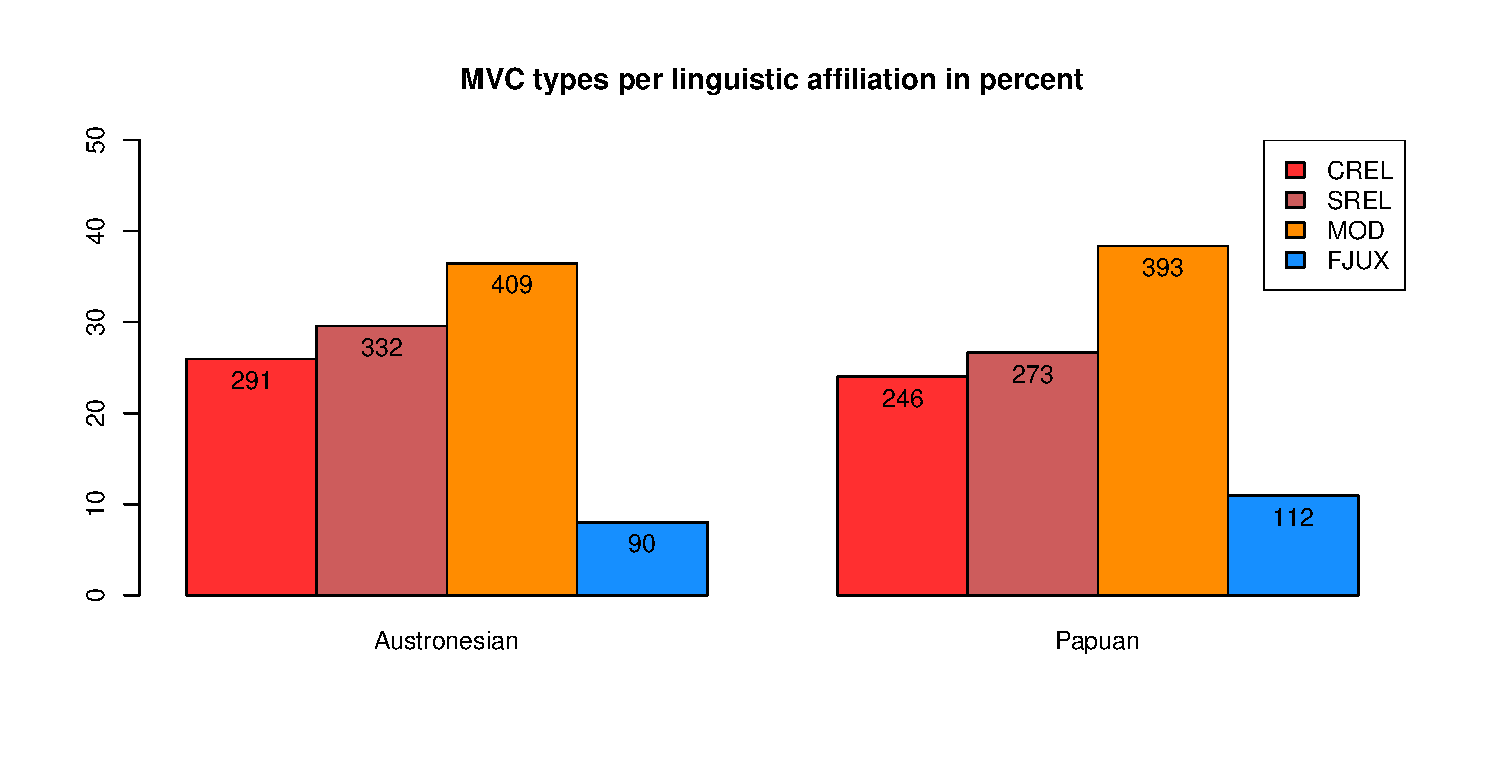
\includegraphics[width=\columnwidth]{../R/plots/Type_Family.eps}
\caption[MVC types per linguistic affiliation in percent]{MVC types per linguistic affiliation in percent. \textsc{crel} = component-relating constructions, \textsc{srel} = stage-relating constructions, \textsc{mod} = modifying constructions, \textsc{fjux} = free juxtaposition constructions. Numbers on top of the bars refer to the number of observations.}\label{fig:type-family}
\end{figure}
\begin{figure}
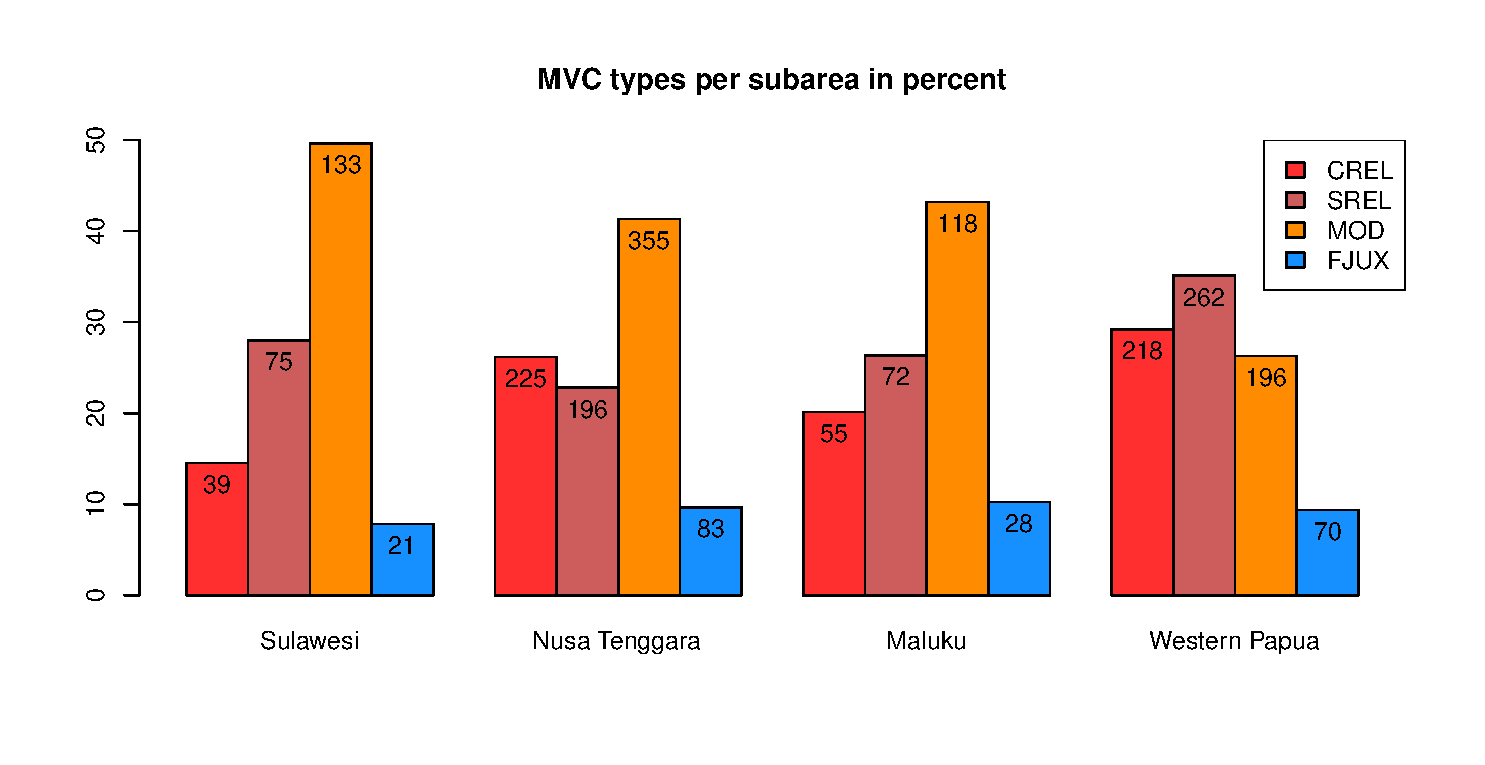
\includegraphics[width=\columnwidth]{../R/plots/Type_Group.eps}
\caption[MVC types per subarea in percent]{MVC types per subarea in percent. \textsc{crel} = component-relating constructions, \textsc{srel} = stage-relating constructions, \textsc{mod} = modifying constructions, \textsc{fjux} = free juxtaposition constructions. Numbers on top of the bars refer to the number of observations.}\label{fig:type-group6}
\end{figure}


The general trend from Figure \ref{fig:type-family} is mirrored in Figure \ref{fig:type-group6} on MVC types per subarea though the ratio is subject to some variation between the subareas. If we just focus on the three western subareas, \textsc{sul}, \textsc{nus}, and \textsc{mal}, a prevalence of modifying constructions is observable, with a peak of almost 50\% in the Sulawesi group. This seems suprising, given that the most prototypical modifying MVCs need to result from a considerable time span of grammaticalisation (think for instance of case-marking MVCs such as give/for, take/with and so on). Thus it would appear that Sulawesi as a subarea is by no means geographically peripheral in the sense that feature innovations emerging from the hotspots of MVC diversity within Wallacea would only weakly percolate into Sulawesi. However, as Table \ref{table:MVCperlang} reveals, the geographically peripheral status of Sulawesi seems to be confirmed by the per language data since there is a sharp split between the northern group (Pendau and Tajio), and the south-eastern group (Tolaki, Muna, and Tukang Besi). It is only in the latter group that modifying constructions indeed score highest. Both Pendau and Tajio have \textsc{mod} constructions to a much lesser extent, with motion constructions from the \textsc{crel} and \textsc{srel} families prevailing instead. The south-eastern languages, on the other hand, only exhibit weak signs of \textsc{crel} use.

The Western Papua group deviates furthest from the overall MVC type ratio. Modifying constructions are less preferred than both \textsc{crel}s and \textsc{srel}s. Stage-relating constructions do especially well with about 35\% of all instances. What remains stable across all four subgroups is the low percentage of recorded \textsc{fjux} constructions.

\begin{table}


\begin{tabular}{lrrrr}
  \lsptoprule
 & CREL & SREL & MOD & FJUX \\ 
  \hline
  Muna &   6 &   2 &  32  &   10  \\ 
  Pendau &  26 &  19 &   5  &   1  \\ 
  Tajio &   4 &  18 &   6  &   4  \\ 
  Tolaki &   3 &  20 &  40  &   2  \\ 
  Tukang Besi &   0 &  16 &  50   &   4 \\ \hline 
  Abui &  10 &  20 &  73  &   6  \\ 
  Alorese &  23 &  17 &   4  &   3  \\ 
  Bunaq &  23 &   6 &  55  &   3  \\ 
  Kaera &  9 &   10 &  4  &   1  \\ 
  Kambera &  15 &   2 &  24  &   3  \\ 
  Klon &  28 &  25 &  40  &   7  \\ 
  Makalero &  17 &   9 &  48  &   2  \\ 
  Teiwa &   18 &  29 &  17  &   21  \\ 
  Tetun &  25 &  19 &  26  &   3  \\ 
  Waima'a &  47 &  44 &  52  &  33  \\ 
  Western Pantar &  10 &  15 &  12  &   1  \\ \hline
  Buru & 10 & 21 & 33 & 4 \\
  Selaru &   3 &   2 &   17  &   2  \\ 
  Taba &   2 &  18 &  22  &   2  \\ 
  Tidore & 33 & 23 & 23 & 13 \\
  Tobelo &   7 &   8 &  23  &   6  \\ \hline
  Abun &  13 &  15 &   1  &   4  \\ 
  Biak &  18 &  31 &  16  &   2  \\ 
  Dusner &  18 &  17 &   9  &  5 \\ 
  Hatam &  18 &  23 &   6  &   2  \\ 
  Inanwatan &  11 &   6 &   4  &   7  \\ 
  Maybrat &  18 &  21 &  30  &   9  \\ 
  Mor &  35 &  23 &   7  &   6  \\ 
  Moskona &   5 &  30 &  38  &   6  \\ 
  Mpur &  15 &  14 &  16  &  17  \\ 
  Sougb &   11 &  19 &   3  &   7 \\ 
  Wooi &  56 &  63 &  66  &   5  \\ 
   \hline
   Total & 537 & 605 & 802 & 202 \\
   \hline
\end{tabular}
\caption[Distribution of attested MVC families per language]{Distribution of attested MVC families per language.}
\label{table:MVCperlang}


\end{table}


Table \ref{table:MVCperlang} gives the numbers of MVC types per language. All languages seem to make use of all four constructional families, with the exception of Tukang Besi for which no component-relating constructions could be found. Although all languages have reported instances of all construction types, different profiles are visible. Some languages, such as Abun or Alorese, show only very few cases of \textsc{mod}s. Other languages have but a few cases of \textsc{crel}s (and, to a lesser extent, \textsc{srel}s) but show a proliferation of \textsc{mod}s, like the group of south-eastern Sulawesi languages already mentioned. Still other languages, such as the two corpus languages Waima'a and Wooi, seem to make good use of all construction families (although \textsc{fjux} scores very low in Wooi). 

Summing up, it is evident that all four techniques of MVC formation are in use all across EI. The factors that may explain the variation in the ratio of MVC types seen above will only become clear if we take a closer look at how the different constructions are distributed across the language sample. Therefore, I will turn to the four MVC families in the remainder of this chapter, providing examples of the different constructions that I assume to be associated with them, and exploring the patterns of use that can be unearthed from the dataset.

\section{Component-relating constructions}

The notion of component here relates to verb strings in which each verb contributes part of the overall semantic structure of the MVC. This is meant to exclude other types of MVCs where the verbs do not enter into a merging relation, i.e. their LS do not undergo a feature matching process. The term component should therefore not be confused with other uses in the literature. For instance, \textcite{dixon2006serial} seems to use the term component verb to refer to any verb that takes part in a serialisation construction. Another conflicting use of the term is the distinction into component vs. narrative SVCs by van Staden and Reesink (2008). It is based upon the notion of `macro event' introduced by \textcite{talmy2000toward} and formally elaborated into a testable category by Bohnemeyer and colleagues (2007, 2011). A construction is said to be `component-relating' when it ``compose[s] so-called `macro-events’
out of smaller units that we refer to as `subevents’", and it is called `narrative' when it ``compose[s] larger event complexes out of macro events" (van Staden and Reesink 2008: 28). Thus the definition of componentiality is essentially derived from an event-based account. 

Componential in my sense of the term only pertains to the features that are present in a set of related constructions throughout the EI languages, specifically these: (i) both (all) verbs belong to the same lexical field (which presupposes in my approach at least a partially identical make-up of LS's), (ii) having a LS that is (partially) identical, the verbs merge part of their features, (iii) if features are overwritten in the merging process, it is features of V$_{1}$ that are preserved and features of V$_{\textsc{fin}}$ that are overwritten. From the criteria previously discussed it has become clear that both \textsc{crel} and \textsc{mod} constructions appear to possess the macro-event property (MEP) as defined by Bohnemeyer et. al. (2007). This is indicated by the fact that these construction types do not allow for partial temporal modification. Hence, while I motivate this constraint by assuming differences in the assignment of hidden event arguments, my understanding of `component-relating' is quite similar to van Staden and Reesink's `component SVCs'. Specifically, I share their insight that among serialisation constructions there are cases that are conceptually packed rather closely while other constructions have parts that behave more like independent subunits.

In the last chapter, I presented an approach to motivate merging of verbal features in a MVC by proposing a set of sublexical structures that might be shared. In order to enable structural merging between verbs of the same lexical field, I introduced empty class predicates \textbf{move'} for motion verbs and \textbf{say'} for speech act verbs. In principle, this approach could be extended to any combination of verbs from identical classes, but as far as I can see it is only motion and speech verbs that behave this way in the EI corpus (with a handful of potential further combinations, see §\ref{sec:other}). 

In what follows, I will quickly preview the different \textsc{crel} constructions found in the EI area, followed by a look at their distribution across the dataset. The subsequent section will then introduce the respective constructions in a bit more detail, and present examples from the corpus. Motion \textsc{crel}s appear in different construals. The most basic construal is motion complex MVCs where a motion verb in V$_1$ (most typically a manner of motion verb) is complemented by a path or ground-denoting verb in V$_2$. This is the standard pattern of feature merging that I  proposed in §\ref{sec:merging} to be the underlying semantic process in \textsc{crel} formation. Several related construals of complex motion seem to have been derived from this pattern. In transport complex MVCs, V$_1$ is a transitive verb of transport. In direction complex MVCs, V$_1$ is also transitive, but does not denote translational motion anymore. Rather, what is denoted is a movement verb to which V$_2$ adds path semantics. Sequitive complex MVCs have a \textsc{follow} verb in V$_1$. What all these constructions have in common is that some kind of \emph{movement} is involved, be it translational motion proper or movement of manipulated objects along some path.

Two more groups of \textsc{crel}s are found in the EI area that are not related to movement. The first construction connects a speech act verb in V$_1$ to a \textsc{say} verb in V$_2$ introducing a propositional argument (what is said). The last group comprises some odd outliers that seem to involve feature merging yet are so infrequent throughout the corpus that no distribution can be traced.

\begin{table}


\begin{tabular}{lrrrrrr}
  \lsptoprule
& \multicolumn{4}{c|}{movement} & & \\
 & {motion} & {direction} & {transport} & {sequitive} & {speech act} & {other}\\  
  \hline
  Austronesian & 166 & 46 & 47 & 9 & 20 & 3 \tabularnewline
  Papuan & 135 & 34 &  36 &  12 & 24 & 5 \tabularnewline
   \hline
  Sulawesi & 25 & 8 & 6 & 0 & 0 & 0 \tabularnewline
  Nusa Tenggara & 144 & 35 & 22 & 7 & 10 & 7 \tabularnewline
  Maluku & 26 & 11 & 4 & 3 & 11 & 0 \tabularnewline 
  Papua & 106 & 26 & 51 & 11 & 23 & 1 \tabularnewline 
\lsptoprule
Total & 301 & 83 & 80 & 21 & 44 & 8 \tabularnewline
\hline
\end{tabular}
\caption[Distribution of \textsc{crel} types]{Distribution of \textsc{crel} types across EI. Note that both subcalculations, i.e. into language family affiliation as well as into areal subgroups, each amount to the total number of observations given in the last row.}
\label{table:CREL_overview}


\end{table}


The impression from the previous section was that \textsc{crel} constructions occur in almost all languages, and are evenly distributed over subareas and language families. If we look more closely at the different \textsc{crel} constructions this picture changes somewhat. Table \ref{table:CREL_overview} above shows the distribution of \textsc{crel} constructions across language families and subareas. The first thing to note is that \textsc{crel} constructions involving movement figure most prominently: 485 out of 537 \textsc{crel} observations involve movement of some kind. Among this group, motion complex constructions are most often attested, making it the default \textsc{crel} construction in the EI dataset. Figure \ref{fig:crel-family} and \ref{fig:crel-group} below illustrate the ratio between \textsc{crel} constructions with regard to language affiliation and subgroup, respectively. Once more, we can discern that linguistic affiliation does not seem to bear on the use of the different constructions. It is only at the subarea level that we can observe considerable differences. The most obvious pattern is a lack of sequitive and speech act constructions in the Sulawesi subgroup. This tallies well with the assumption already mentioned that Sulwesi, forming the western periphery of an assumed Wallacea Sprachbund, does not have the full range of MVC constructions in use. The other three subareas each show all \textsc{crel} constructions, although there are more observations of the minor constructions in Maluku and Western Papua languages than in the Nusa Tenggara languages.

\begin{figure}
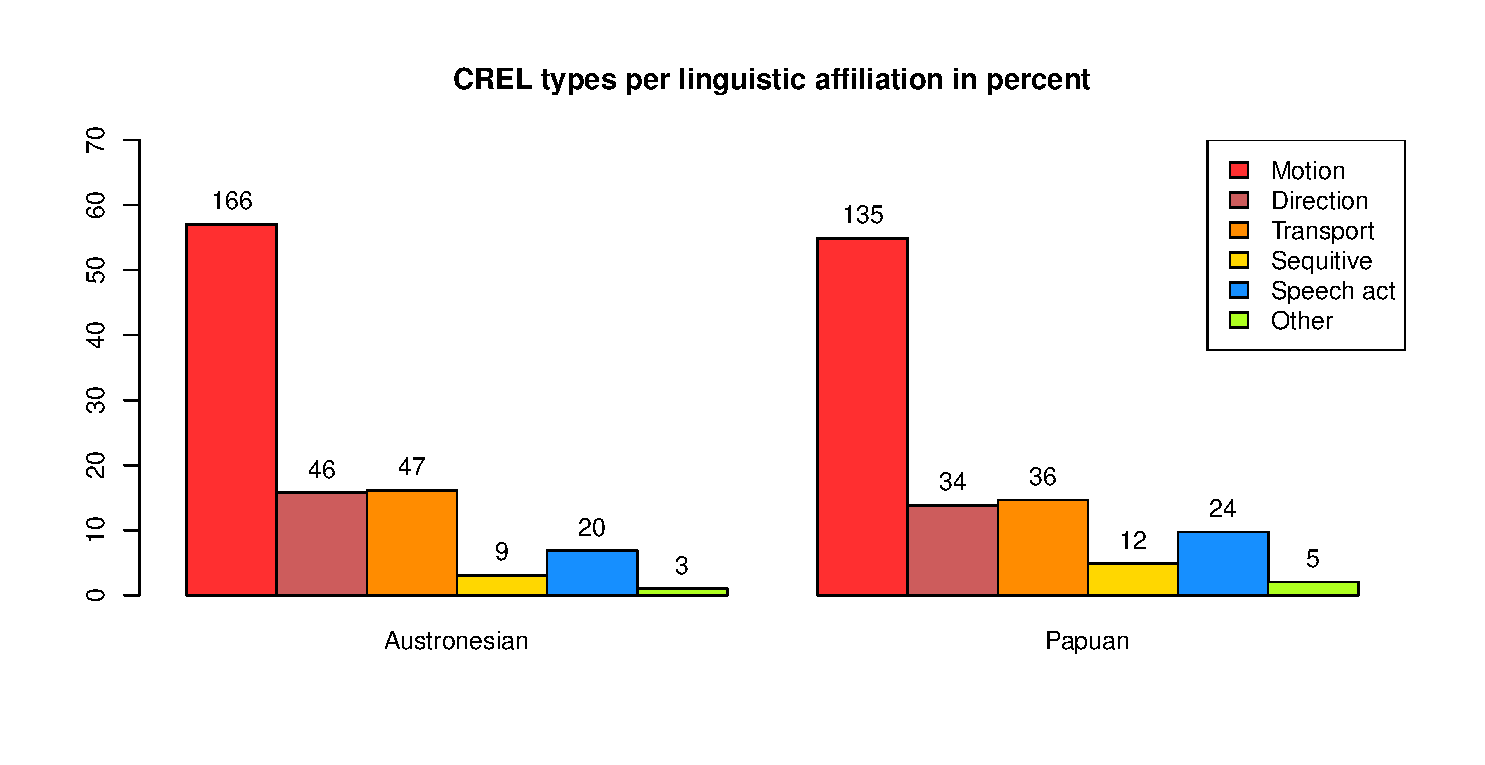
\includegraphics[width=\columnwidth]{../R/plots/CREL_Family.eps}
\caption[CREL types per linguistic affiliation in percent]{CREL types per linguistic affiliation in percent. Numbers on top of the bars refer to the number of observations in the dataset.}\label{fig:crel-family}
\end{figure}
\begin{figure}
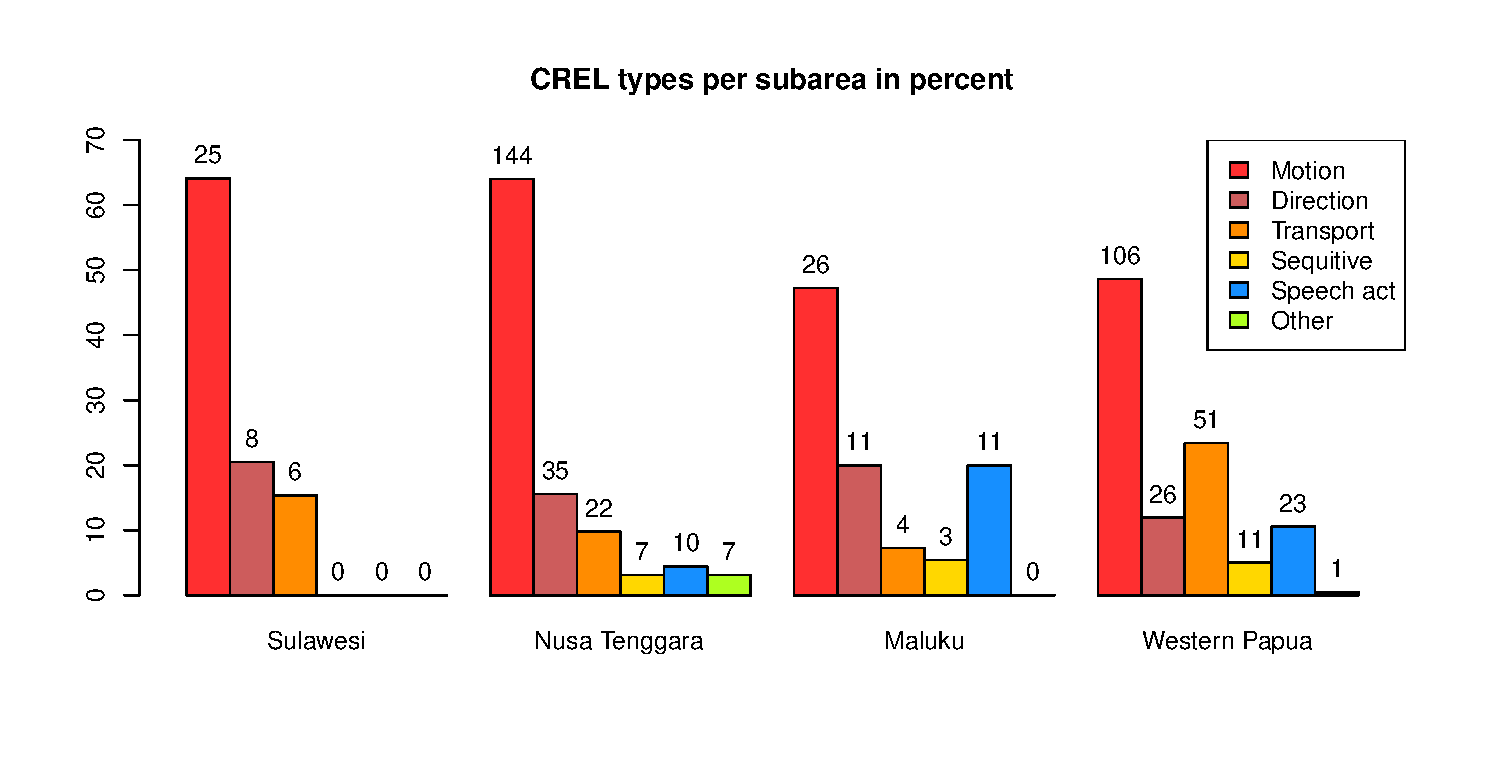
\includegraphics[width=\columnwidth]{../R/plots/CREL_Group.eps}
\caption[CREL types per subarea in percent]{CREL types per subarea in percent. Numbers on top of the bars refer to the number of observations in the dataset.}\label{fig:crel-group}
\end{figure}


Table \ref{table:crel_language} below shows the distribution of attested CREL construction types per language. The different constructions are quite evenly distributed within the four subgroups showing that they are in fact widespread throughout the subareas, and do not just cluster in some exceptional language. If a language makes use of feature merging resulting in \textsc{crel}s, there are always motion complex constructions among it. Direction, transport, and sequitive \textsc{crel}s all involve transitive verbs in V$_1$ position, and the figures for these constructions are much lower than for motion complexes. What is more, the occurrence of the 'minor' movement constructions appears to entail the use of the basic motion complex construction. That is, there are no languages for which only minor movement constructions are attested. This supports the assumption that the motion complex construction is the most basic one, possibly the construction from which the minor ones are derived. Another entailment suggested by the EI data is that if a language shows sequitive \textsc{crel}s then it also tends to have attested direction and transport \textsc{crel}s (with the exception of Inanwatan and Sougb). Direction and transport, on the other hand, seem not directly related to one another as either construction may occur without the other.

\begin{table}


\begin{tabular}{lrrrrrr}
\lsptoprule
& \multicolumn{4}{c|}{movement} & & \\
 & {motion} & {direction} & {transport} & {sequitive} & {speech act} & {other}\\ 
  \hline
  Muna &   5 &   0 &   1 &   0 &   0 &   0  \\ 
  Pendau &  15 &   7 &   4 &   0 &   0 &   0 \\ 
  Tajio &   3 &   0 &   1 &   0 &   0 &   0 \\ 
  Tolaki &   2 &   1 &   0 &   0 &   0 &   0 \\ 
  Tukang Besi & 0 & 0 & 0 & 0 & 0 & 0 \\ \hline
  Abui &   4 &   3 &   1 &   2 &   0 &   0 \\ 
  Alorese &  19 &   1 &   1 &   1 &   1 &   0 \\ 
  Bunaq &  18 &   5 &   0 &   0 &   0 &   0 \\ 
  Kaera &   7 &   0 &   2 &   0 &   0 &   0 \\ 
  Kambera &   3 &   4 &   4 &   1 &   1 &   2 \\ 
  Klon &  21 &   0 &   0 &   0 &   4 &   3 \\ 
  Makalero &  11 &   1 &   4 &   0 &   1 & 0  \\ 
  Teiwa &   14 &   0 &   4 &   0 &   0 &   0 \\ 
  Tetun &  16 &   4 &   4 &   0 &   0 &   1 \\ 
  Waima'a &  23 &  17 &   2 &   3 &   2 &   0 \\ 
  Western Pantar &   8 &   0 &   0 &   0 &   1 &   1 \\ \hline
  Buru & 8 & 1 & 0 & 0 & 1 & 0 \\
  Selaru &   1 &   0 &   0 &   0 &   2 &   0 \\ 
  Taba &   2 &   0 &   0 &   0 &   0 &   0 \\ 
  Tidore & 13 & 9 & 4 & 3 & 4 & 0 \\
  Tobelo &   2 &   1 &   0 &   0 &   4 &   0 \\ \hline
  Abun &   4 &   3 &   6 &   0 &   0 &   0 \\ 
  Biak &   9 &   3 &   5 &   1 &   0 &   0 \\ 
  Dusner &  11 &   0 &   4 &   1 &   2 &   0 \\ 
  Hatam &   5 &   4 &   9 &   0 &   0 &   0 \\ 
  Inanwatan &   4 &   0 &   4 &   2 &   0 &   1 \\ 
  Maybrat &   8 &   4 &   0 &   0 &   6 &   0 \\ 
  Mor &  15 &   2 &   8 &   2 &   8 &   0 \\ 
  Moskona &   4 &   0 &   1 &   0 &   0 &   0 \\ 
  Mpur &   4 &   4 &   0 &   5 &   2 &   0 \\ 
  Sougb &   8 &   0 &   1 &   0 &   2 &   0 \\ 
  Wooi &  34 &   6 &  13 &   0 &   3 &   0 \\ 
   \hline
   Total & 301 & 80 & 83 & 21 & 44 & 8 \\
   \hline
\end{tabular}
\caption{Distribution of attested CREL construction types per language}
\label{table:crel_language}


\end{table}


Now, having arrived at a MVC analysis driven by semantic interaction techniques as introduced in chapter \ref{ch:sem}, we can bring the morphosyntactic parameters from chapter \ref{ch:gram} back into play. Table \ref{table:crel_formal} illustrates that the \textsc{crel} constructions display a much more homogeneous picture with regard to morphosyntactic properties than has been found for the whole dataset in chapter \ref{ch:gram}. In terms of referentiality, the same-subject configuration is strongly prevalent in all \textsc{crel} constructions, except for direction complexes. This does not come as a surprise, given that in direction complexes, there is typically an argument-switch involved (see discussion below in section §\ref{sec:direction}). This variation in referentiality encoding correlates with a tendency of direction complexes (as well as the other movement constructions) towards inflecting only the starting verb of the series. Uninflected V$_2$ in direction complexes thus leads to some degree of coding ambiguity with regard to argument interaction. This helps explain the wide range of referentiality values annotated.

The headedness patterns from Table \ref{table:crel_formal} point out another notable tendency. In all movement constructions it is V$_1$ that is allocated the main inflectional load. The ``1" inflection pattern is predominant across the board, and outnumbers the ``B" pattern. Associating information on verbal categories, such as TAM or subject indexing, to only one head creates an asymmetry that can be interpreted as lending prominence to V$_1$. This is basically in line with the criterion introduced in section §\ref{sec:criteria_mvcs} above, namely that in \textsc{crel} it is V$_1$ that preserves its verbal properties rather than the subsequent verbs\footnote{Note that these figures are slightly biased towards the ``1" pattern as I interpreted directional verboids in post-verbal position as verbs, for instance in languages that I am familiar with (Wooi, Waima'a) or where the lexeme in question can either diachronically or synchronically be traced back to a verb root (think of Wooi \textit{ma} from the very first example in chapter \ref{ch:introduction}). Alternative analyses might reanalyse some such strings into verb - (directional) particle constructions, and arrive at lower numbers of ``1" patterns.}. This prominence shift is, however, not visible in speech complex constructions, as these appear to favour the ``B" pattern.

\begin{table}
\centering

\begin{tabular}{rrrrrr}
  \lsptoprule
Referentiality & S & SO & D & A & E \\ 
  \hline
motion complex & 300 &   0 &   0 &   0 &   1 \\ 
  direction complex &  20 &   5 &  33 &   0 &  22 \\ 
  transport complex &  80 &   0 &   2 &   1 &   0 \\ 
  sequitive complex &  19 &   0 &   2 &   0 &   0 \\ 
  speech act complex &  44 &   0 &   0 &   0 &   0 \\ 
  other &   8 &   0 &   0 &   0 &   0 \\ 
   \hline
 \\
  \hline
Headedness & B & 1 & 2 & S & N \\ 
  \hline
motion complex &  39 &  83 &   2 &  10 &  14 \\ 
  direction complex &  12 &  22 &   0 &   5 &   6 \\ 
  transport complex &  15 &  32 &   4 &   4 &   4 \\ 
  sequitive complex &   3 &   6 &   2 &   2 &   2 \\ 
  speech act complex &  24 &   4 &   1 &   1 &   4 \\ 
  other &   0 &   0 &   1 &   2 &   0 \\ 
   \hline
 \\
  \hline
Contiguity & W & C & 1 & 2 & 3 \\ 
  \hline
motion complex &   8 & 241 &  46 &   5 &   1 \\ 
  direction complex &   0 &  54 &  24 &   2 &   0 \\ 
  transport complex &   4 &  47 &  31 &   0 &   1 \\ 
  sequitive complex &   2 &  17 &   2 &   0 &   0 \\ 
  speech act complex &   0 &  34 &  10 &   0 &   0 \\ 
  other &   1 &   7 &   0 &   0 &   0 \\ 
   \hline
\end{tabular}
\caption[Morphosyntactic properties of \textsc{crel} constructions]{Morphosyntactic properties of \textsc{crel} constructions in EI. Table components from top to bottom refer to referentiality (see section §\ref{sec:argumentstructure}), headedness (see section \ref{sec:headedness}), and contiguity (see section \ref{sec:contiguity}), respectively.}
\label{table:crel_formal}

\end{table}


In the following sections, I will briefly present the \textsc{crel} constructions one by one. The purpose of these sections is to provide examples from all subareas where the construction is attested.

\subsection{Motion complex} \label{sec:motioncomplex}

Motion complex constructions form the largest subgroup of the \textsc{crel} class with 301 attested data points out of 537 instances of \textsc{crel}s and 2146 instances of MVCs in total. The basic distributional properties are the same as for the \textsc{crel}s in general, since every language in the corpus that has \textsc{crel} constructions also has motion complexes. Table \ref{table:basiccrelmotion} gives the respective numbers as well as the general template. A motion complex is made up of two or more verbs with each verb belonging to the lexical field of motion verbs.

\begin{table}


\begin{tabular}{ll}
\lsptoprule
Feature&Value\tabularnewline
\hline
Template&V1 \textsc{motion} -- V2 \textsc{motion}\tabularnewline
No. of attested instances& 301/2146 \tabularnewline
No. of attested languages& 31/32 (not attested: Tukang Besi) \tabularnewline
Distribution across areas& \textsc{sul} (4/5), \textsc{nus} (11/11), \textsc{mal} (5/5), \textsc{pap} (11/11) \tabularnewline
Distribution across families& \textsc{pap} (16), \textsc{aus} (15) \tabularnewline
\hline
\end{tabular}
\caption[Template and basic distribution of \textsc{crel} motion complexes]{Template and basic distribution of \textsc{crel} motion complexes in the EI data set. First verb mostly intransitive with few exceptions, second verb intransitive or transitive}
\label{table:basiccrelmotion}
\end{table}


The following examples (\ref{Pendau24}) to (\ref{Hatam001}) are from all four subareas, and show the typical appearance of motion complexes in EI. The first verb tends to be intransitive (with only a handful of exceptions, for instance \textsc{leave}, \textsc{cross}, or \textsc{reach} verbs taking a ground argument) and often refers to the way the motion is carried out, or gives part of the path information needed to project the whole motion vector. The verb in V$_{\textsc{fin}}$ is most often a path verb. In the Pendau example (\ref{Pendau24}) the moving referent undergoes a non-volitional motion event on a vertical projection plane. Example (\ref{Alorese001}) from Alorese shows a manner of motion verb followed again by a path verb, this time opening up a deictic vector directed towards the speaker origo. This example is somewhat unusual in that the moving referent is inanimate (most cases have animate actors performing some motion at will). The next example has another common combination of motion verbs with a reverse path verb in V$_{2}$ position and a vertical path verb in V$_{1}$. Note that the corpus also contains motion complexes with exactly the opposite order where a \textsc{return} verb is followed by a vertical or horizontal path verb. These cases are, however, restricted to combinations of motion verbs that both convey path semantics. Non-path-denoting motion verbs never appear in V$_1$, supporting the assumption that manner is placed before path in a motion complex. The last example from Hatam has a potentially transitive ground-denoting verb in V$_{1}$ which, however, need not be produced with a ground NP. In such cases like (\ref{Hatam001}) I interpret the function of contained path verbs (\textsc{enter}, \textsc{exit}) as emphasizing additional information on the path rather than introducing a ground referent which is not overtly specified.

\ea \label{Pendau24}
%\begingl[glhangstyle=none]
%\rightcomment{{\small \textbf{Pendau} \textsc{sul}}}
\gll odo moo \textbf{nanabumo} \textbf{manyau} + rilalong nuapi \\
odo moo no-nabu=mo ma-nyau ri=lalong nu=api \\
\glc monkey this \acs{st}.\acs{rls}-fall=\acs{comp} \acs{irr}-go.down \acs{loc}=inside \acs{cn}=fire \\
\glft `This monkey fell down into the fire.' 
\trailingcitation{(Quick 2007: 344)}\\ 
\z
\xe

\ea \label{Alorese001}
%\begingl
%\rightcomment{{\small \textbf{Alorese} \textsc{nus}}}
\gll terus, kaju fatang \textbf{nepi} \textbf{mene} \\
then wood sea float come \\
\glft `Then a piece of wood came floating (towards us).' \trailingcitation{(Klamer 2011: 63)}\\ 
\z
\xe

\ea \label{Taba002}
%\begingl
%\rightcomment{{\small \textbf{Taba} \textsc{mal}}}
\gll \textbf{ncopang} \textbf{nmul} hu \\
n=sopang n=mul hu \\
\glc \acs{3}\acs{sg}=descend \acs{3}\acs{sg}=return \acs{cont} \\
\glft `(S)he's still coming back down.' \trailingcitation{(Bowden 2001: 295)}\\ 
\z
\xe

\ea \label{Hatam001}
%\begingl
%\rightcomment{{\small \textbf{Hatam} \textsc{pap}}}
\gll \textbf{a-coi} \textbf{kwei} \\
\acs{2}\acs{sg}-enter come \\
\glft `Come in.' (= invitation to visitor) \trailingcitation{(Reesink 1999: 100)}\\ 
\z
\xe

The four examples are also typical motion complexes in terms of their morphosyntactic behaviour, as we have already seen from Table \ref{table:crel_formal}. \textsc{crel} motion complexes can basically appear in all inflection patterns. This is reflected by the examples: in (\ref{Pendau24}) and (\ref{Taba002}) both verbs take inflectional marking\footnote{The Sulawesi case is a bit more complex inasmuch as a small group of motion verbs in V$_{\textsc{fin}}$ shows defective inflectional behaviour. In Pendau, only \textit{nyau} can occur with a prefix, either taking the form \textit{ma-nyau} or \textit{menyau} (from \textit{M-pe-nyau} \textsc{irr}-\textsc{sf/dyn}-go.down, see ex. (55) in Quick 2007: 342 and discussion on p.344 incl. footnote 8). As Quick's examples and discussion show, there is no realis form that would match \textsc{irr} \textit{ma-nyau}. A similar form occurs in neighbouring Tajio with \textit{minyau} which could be analysed as a lexicalised former irrealis form. However, contemporary Tajio also lacks a realis counterpart (see Mayani 2013:136).}, example (\ref{Hatam001}) shows inflection only on the first verb, and in Alorese (\ref{Alorese001}) both verbs remain bare. The choice of inflection pattern is influenced by two factors: (i) the overall grammatical system of the language, and (ii) dominance of the first verb. I assume that the first factor is a relative one that is particularly influential in areas with high levels of mutual linguistic contact. The second factor seems to be a more general characteristic of motion verb construals in the EI area, and draws supporting evidence from two facts. First, as noted earlier, in feature merging it is features of V1 that are preserved (\textsc{fall} in V$_{1}$ passes on features of non-volitionality while \textsc{fall} in V$_{\textsc{fin}}$ does not). Second, the diachronic development in motion verb construals seems to suggest a gradual decline of verbal properties in V$_{\textsc{fin}}$, leading to the eventual loss of inflection and the ultimate formation of a class of directional operators. This process is well-known from many languages (see for instance Aikhenvald 2006: 31).

Inanwatan is the only language in the corpus that really seems to have developed a motion construction in which the second verb bears the morphosyntactic locus. Consider the following two examples.

\ea \label{Inanwatan16}
%\begingl[glhangstyle=none]
%\rightcomment{{\small \textbf{Inanwatan} \textsc{pap}}}
\gll mé-se-i ewáiwa + nóe-we-i-di \\
\acs{3}\acs{subj}-walk-\acs{pst}.\acs{m} and go.out-\acs{3}\acs{subj}-descend-\acs{pst}.\acs{m} \\
\glft `(and) he went on and on and he arrived' \trailingcitation{{\small (de Vries 2004: 49)}}\\ 
\z
\xe

\ea \label{Inanwatan20}
%\begingl
\gll mé-de-wo-i ewáiwa \\
\acs{3}\acs{subj}-go.across-come-\acs{pst}.\acs{sg}.\acs{m} and \\
\glft `he came across and [...]' \trailingcitation{{\small (de Vries 2004: 55f.)}}\\ 
\z
\xe

The first example in (\ref{Inanwatan16}) depicts the construction that I coded as ``2": the first motion verb, \textit{noé} `go out', is preposed to the finite verb complex, \textit{we-i-di} `he descended', as a bare stem. Another pattern, where both verbs share the inflection set of prefix and suffix, is illustrated in (\ref{Inanwatan20}). Here, both motion verbs can be conceived as inflected (`shared' inflection in my terms). The fact that Inanwatan affords two different construals of motion complexes could indicate that the deictic path verb \textit{wo} `come' (and maybe others more in this construction) has already begun to lose part of its verbal properties in this context, moving along a grammaticalisation path that ultimately leads to the formation of a class of non-verbal directional elements. Inanwatan \textit{wo} would thus generally fit into the pattern of deverbalisation of \textsc{go} and \textsc{come} verbs in many EI languages.

Two languages in the \textsc{pap} subarea, Inanwatan and Sougb, allow motion complex construals within one phonological word. The Inanwatan examples (\ref{Inanwatan16}) and (\ref{Inanwatan20}) above have already illustrated this type and the figures for Inanwatan indicate that the construction pattern seems the only choice for motion complex construals in that language. Sougb is a bit different as it belongs to the group of languages with more than one attested contiguity value. The reason for this is that Sougb \textit{da} (from \textit{eda} `go') and \textit{in} (from \textit{en} `come'), the only two motion verbs attested in V$_{\textsc{fin}}$, behave like clitics: they seem to attach to V$_{1}$ unless a direct object NP or a goal NP intervenes in which case they attach to the NP. Note, however, that the source PP in (\ref{Sougb002a}) does not attract the clitic verb. The Sougb case is illustrated by the following triad:

\pex \label{Sougb002}
\a \label{Sougb002a}
%\begingl
%\rightcomment{{\small \textbf{Sougb} \textsc{pap}}}
\gll godeh hom g-ougb-\textbf{da} dau m-ena \\
child one \acs{nom}-run-go from \acs{3}\acs{sg}-father \\
\glft `a son who ran away from his father' \trailingcitation{{\small (Reesink 2002a: 200)}}\\ 
\z
\a
%\begingl
\gll yen y-aiga duhu-\textbf{da} \\ 
you \acs{2}\acs{pl}-cross water-go \\
\glft `cross the river' \trailingcitation{{\small (Reesink 2002a: 226)}}\\ 
\z
\a
%\begingl
\gll en esogw-esa se duhu aud en-\textbf{da} \\ 
he jump-stand at water to him-go \\
\glft `he jumped into the water towards him' \trailingcitation{{\small (Reesink 2002a: 226)}}\\ 
\z
\xe

Referentiality in motion complexes remains ``S" throughout all cases, as shown in Table \ref{table:crel_formal} above. In principle, it is not clear why there are no languages that use the predicate-argument reanalysis scenario instead (in which the modifier verb takes the whole main verb predication as its argument). This pattern occurs in Southeast Sulawesi languages with construals of temporal verboids. If a temporal verboid, as shown in example (\ref{Muna018}) from Muna, can take as its subject the second VP, one might wonder why this is not also an option in motion complexes, especially if the second verb is a path verb that has already lost part of its verbal properties. A construal like `it is usual (that) I swim' could then be paralleled by construals such as `it is hither I go/my going is hither'. Yet no such option is attested in the data set except for one construction in Mpur, illustrated in (\ref{Mpur061}) below.

\ea \label{Muna018}
%\begingl
%\rightcomment{{\small \textbf{Muna} \textsc{sul}}}
\gll no-rea a-leni \\
\acs{3}\acs{sg}.\acs{rls}-usual \acs{1}\acs{sg}.\acs{rls}-swim \\
\glft `I usually swim' \trailingcitation{{\small (van den Berg 1989: 236f.)}}\\ 
\z
\xe

\ea \label{Mpur061}
%\begingl
%\rightcomment{{\small \textbf{Mpur} \textsc{pap}}}
\gll bisa n-dokwa na n-aw a-ye' \\
can \acs{1}\acs{sg}-bring for \acs{3}\acs{sg}.\acs{f}-run \acs{3}\acs{sg}.\acs{m}-out \\
\glft `bring (something) to get her out' \trailingcitation{{\small (Odé 2002: 101)}}\\ 
\z
\xe

The motion complex \textit{n-aw a-ye'} here is construed as a purpose complement marked as such by \textit{na}. Mpur has overt gender distinction between masculine and feminine in third person singular. In (\ref{Mpur061}) we observe a mismatch in gender marking between the first verb and the second which points to the conclusion that the subject of the outward movement denoted by \textit{ye'} cannot be the female runner from V$_{1}$. The only other interpretation that seems available here is that \textsc{3sg.m} can be used as a default marker for sentential arguments in Mpur, taking the first VP \textit{n-aw} as a subject here. Predicate-argument reanalysis is a feature that is further attested in the Bird's Head area, for instance in argument-marking constructions from Maybrat, in sequentialiser constructions from Moi (not part of the corpus), or manner serialisation in Moskona where the zero-marked manner verb is interpreted to take the entire predicate of the main verb as its subject (Gravelle 2010: 299f.). 

Summarising so far, we have seen that despite the large amount of data points from almost all EI languages, motion complexes are moulded into a fairly consistent form. From a formal perspective we can state that the verbs tend to stand adjacent to each other and display co-referential participant marking ('same subject'). If there is verbal inflection then it is the first verb that tends to receive it except for the \textsc{nus} subarea where constructions (and languages) without clear inflection patterns predominate. From a semantic viewpoint, the stable factor is that the verbs all belong to the lexical field of motion verbs and merge part of their LS. The bulk of constructions has the following order: V$_{1}$ refers to the act of moving (predominantly lexicalised manner of motion) while V$_{\textsc{fin}}$ contributes information on the way the motion event unfolds through space and time. Yet, we have already seen other examples (e.g. the Inanwatan examples in (\ref{Inanwatan16})) where V$_{1}$ presents path information and/or introduces (covert) ground referents (`go.out', `go.across') which the motion event is set in relation to. This suggests that there is a good deal of variation as to which motion verb class appears in which constructional slots, in particular when language-specific constituent order constraints (as AOV in Inanwatan) clashes with the order dominant verb - modifier verb in motion complexes. The most crucial ordering principle, however, that I take to be at the heart of motion complex constructions, \textsc{manner} before \textsc{path}, is well-attested and not subject to any change in order. This constraint offers an interesting perspective on the framing discussion in complex motion expressions (as already briefly mentioned in section §\ref{sec:sem-templates}). Talmy's (1985, 2000) two-way typology has recently been expanded into a three-way typology, accomodating serialising languages as an independent framing type (called equipollently-framed by Slobin 2004). While the nature of motion framing in SVCs is still under discussion, it is quite remarkable that both satellite-framed and serialising languages show a strong preference to place \textsc{manner} before \textsc{path} (see Ameka and Essegbey 2013 for a recent overview).

\subsection{Direction complex} \label{sec:direction}
Direction complexes bear a resemblance to motion complexes as well as to transport complexes. With both construction types they share the (predominant) use of motion path verbs in V$_{\textsc{fin}}$ defining a trajectory of the motion event. Another feature they share with transport complexes is that the first verb in a directon complex is in most cases transitive (only directed perception verbs such as \textsc{look} deviate from this pattern). They differ, however, from both previous construction types in that the motion event is no longer understood as translational motion but as a derived motion concept, capturing body part movement as well as stimulus perception vectors. Table \ref{table:basiccreldir} has the basic features of direction complexes in the EI area.

\begin{table}


\begin{tabular}{ll}
\lsptoprule
Feature&Value\tabularnewline
\hline
Template&V1 \textsc{action/perception$_{\textsc{tr}}$} - V2 \textsc{motion$_\textsc{intr}$}\tabularnewline
No. of attested instances& 80/2146 \tabularnewline
No. of attested languages& 19/32 \tabularnewline
Distribution across areas& \textsc{sul} (2/5), \textsc{nus} (7/11), \textsc{mal} (3/5), \textsc{pap} (7/11) \tabularnewline
Distribution across families& \textsc{pap} (9), \textsc{aus} (10) \tabularnewline
\hline
\end{tabular}
\caption[Template and basic distribution of \textsc{crel} direction complexes]{Template and basic distribution of \textsc{crel} direction complexes in the EI data set. First verb denotes object manipulation/relocation or perception, second verb contributes motion path semantics.}
\label{table:basiccreldir}
\end{table}
 

The following examples present typical cases of direction complexes from the \textsc{sul}, \textsc{nus}, and \textsc{pap} subareas (the only example from \textsc{mal} will be discussed further below). All three of them make use of a vertical or deictic path verb in V$_{\textsc{fin}}$, yet the event does not encode translational motion of the actor. In (\ref{Pendau027}) the path verb \textit{manyau} denotes a downward trajectory of some instrument. Pendau is the only \textsc{sul} language with several cases of attested direction complexes, both in combination with verbs of object manipulation ('cast', 'slash') and with perception verbs ('stare', 'look'). Example (\ref{Abui061}) from Abui illustrates a directed perception event where the vertical path verb \textit{mara} adds the vector that spans between the experiencer (introduced here by grammaticalized \textit{ng} 'see') and his visual focus. Again it is the constructional setting that pre-empts the motion verb from being interpreted as an act of literal motion. The last example is from the \textsc{pap} subarea and shows yet another way of combining an action verb with a motion path verb. \textit{tu} is a verb of object relocation rather than object manipulation but serves well in a direction complex. Other examples from Maybrat involve the verb \textit{ai} 'hit'.

\ea \label{Pendau027}
%\begingl[glhangstyle=none]
%\rightcomment{{\small \textbf{Pendau} \textsc{sul}}}
\gll nitoto'a'onyo manyau + riba'i nirapinyo \\
ni-toto'-a'=nyo ma-nyau ri=ba'i ni=rapi=nyo \\
\glc \acs{iv}.\acs{rls}-slash-\acs{tz}=\acs{3}\acs{sg}.\acs{gen} \acs{ug}.\acs{irr}-go.down \acs{loc}=head \acs{pn}.\acs{gen}=spouse=\acs{3}\acs{sg}.\acs{gen} \\
\glft `He slashed it down into his wife's head' \trailingcitation{{\small (Quick 2007:346)}}\\ 
\z
\xe

\ea \label{Abui061}
%\begingl
%\rightcomment{{\small \textbf{Abui} \textsc{nus}}}
\gll di=ng wahai mara \\
\acs{3}\acs{act}=see look go.up.\acs{cont} \\
\glft ‘he looks up’ \trailingcitation{Kratochvíl 2007: 363}\\ 
\z
\xe

\ea \label{Maybrat102}
%\begingl
%\rightcomment{{\small \textbf{Maybrat} \textsc{pap}}}
\gll t-tu aya m-amo cerek a \\
\acs{1}\acs{sg}-pour water \acs{3}\acs{u}-go thermos.flask \acs{q} \\
\glft `Should I pour water into the thermos flask?' \trailingcitation{{\small (Dol 2007: 215)}}\\ 
\z
\xe

The last example from Maybrat is reminiscent of ambient serialisation inasmuch as the referential alignment shows a mismatch between the subject of V$_{1}$ and V$_{\textsc{fin}}$. Dol explicitly discusses this construction type as shared argument construction and interprets the object of V$_{1}$ as subject of V$_{\textsc{fin}}$ (Dol 2007: 217), that is, it is the water that `goes' into the thermos flask not the pouring of the water as would be the case with ambient marking. 

One distributional property of direction complex constructions that is particularily striking is that all instances of direction complexes encoded as double-head inflection (``B" pattern) only feature verbs of object manipulation or relocation. There is not one instance of double marking with perception constructions. This raises the following question: what is the (understood) subject of the motion path verb in V$_{\textsc{fin}}$? Is it the experiencer, the stimulus (with transitive perception verbs), the whole predication of perceiving something, or maybe none at all as the motion verbs might have already lost part of their verbhood in that particular construction? An analysis of the EI dataset shows that all languages that have both types (action and perception) attested either do not use verbal inflection at all (Alorese, Waima'a), or inflect the initial verb only (Biak, Wooi), or have unregular inflection patterns not generally suitable to characterise constructions (Pendau, Abui). Therefore we cannot at this point make any prediction on the identity of the second subject argument in direction complexes. Another feature that becomes evident is that all languages that allow for perceptional direction complexes are in fact Austronesian languages (except for the one example from Abui illustrated in (\ref{Abui061}) above). If this tendency proved to be true with more data, one could state that direction complexes of the perception type are more common in Austronesian than in Papuan languages. On the other hand might a closer inspection of larger amounts of data generally reveal more languages with both constructions. This is foreshadowed by the fact that in both corpus languages for which more data have been collected, Waima'a and Wooi, both constructions were found to be present.

A final example that I want to present here is the (only) one from Tobelo. 

\ea \label{Tobelo033}
%\begingl
%\rightcomment{{\small \textbf{Tobelo} \textsc{mal}}}
\gll t-a-ika t-i-tauru no-maoko la no-ma-tagi \\
\acs{1}-\acs{vf}-\acs{all} \acs{1}-\acs{3}\acs{m}-pull \acs{2}-stand \acs{conj} \acs{2}-\acs{refl}-walk \\
\glft `I pulled him up so that he could walk' \trailingcitation{{\small (Holton 2003: 63)}}\\ 
\z
\xe

This example is unusual in at least two ways (ignoring the resultant phase denoted by the third verb \textit{no-maoko}): first, the order action verb - motion path verb is reversed, a pattern that we do not find in the other languages. And second, the motion path verb seems to be grammatical in nature rather than a full lexical item (capable of predicating a simplex predicate). Such instances at best constitute peripheral cases of direction complexes, if at all.

\subsection{Transport complex} \label{sec:transport}

The next subtype of \textsc{crel} constructions consists of a verb of transport, such as \textsc{bring}, \textsc{hold}, \textsc{carry}, or \textsc{bear}, which is complemented by a motion path verb in V$_2$. The combination of verbs is interpreted as denoting an act of translational motion where the actor is in possession of an object and relocates it by way of changing his/her position in the landscape of discourse. Table \ref{table:basiccreltransport} lists the basic properties of transport complexes in the EI languages. 

\begin{table}


\begin{tabular}{ll}
\lsptoprule
Feature&Value\tabularnewline
\hline
Template&V1 \textsc{transport$_{\textsc{tr}}$} * V2 \textsc{motion}\tabularnewline
No. of attested instances& 83/2146 \tabularnewline
No. of attested languages& 21/32 \tabularnewline
Distribution across areas& \textsc{sul} (3/5), \textsc{nus} (8/11), \textsc{mal} (1/5), \textsc{pap} (9/11) \tabularnewline
Distribution across families& \textsc{pap} (11), \textsc{aus} (10) \tabularnewline
\hline
\end{tabular}
\caption[Template and basic distribution of \textsc{crel} transport complexes]{Template and basic distribution of \textsc{crel} transport complexes in the EI data set. The first verb encodes possession and motion, the second verb contributes further motion components (predominantly path). The asterisk indicates that the order transport - motion is reversed in a small number of constructions}
\label{table:basiccreltransport}
\end{table}
 

Here are some examples from different subareas. The first example in (\ref{Tajio023}) is from Sulawesi showing a \textsc{bring} verb in V$_{1}$ followed by a deictic path verb. Example (\ref{Makalero089}) uses another strategy to encode a transport event: here it is the handling verb \textit{mei} 'take' that denotes the translocation of the item in question (which is a group of people here, it seems). More typical for transport constructions would be inanimate referents such as the tobacco in (\ref{Tajio023})). And (\ref{Hatam066}) from Hatam shows yet another option by using a \textsc{hold} verb again combined with a deictic motion verb in V$_{\textsc{fin}}$.

\ea \label{Tajio023}
%\begingl
%\rightcomment{{\small \textbf{Tajio} \textsc{sul}}}
\gll vava minyei ba i ulu tabako=mu \\
bring go.here please \acs{loc} first tobacco=\acs{2}\acs{sg}.\acs{poss} \\
\glft ‘Give me first your tobacco, please' \trailingcitation{{\small (Mayani 2013: 294)}}\\ 
\z
\xe

\ea \label{Makalero089}
%\begingl
%\rightcomment{{\small \textbf{Makalero} \textsc{nus}}}
\gll ...ain=isi hai mei ma’u \\
\acs{quot}=\acs{lnk}\acs{2} \acs{nsit} take come \\
\glft '[direct speech] so she brought
them' \trailingcitation{{\small (Huber 2011: 206)}}\\ 
\z
\xe

\ea \label{Hatam066}
%\begingl
%\rightcomment{{\small \textbf{Hatam} \textsc{pap}}}
\gll yoni i-krau munggwom kwei big \\
they \acs{3}\acs{pl}-hold child come not \\
\glft `They don't bring the child(ren)' (lit. They don't hold the child(ren) hither) \trailingcitation{{\small (Reesink 1999: 109)}}\\ 
\z
\xe

Let us consider the evidence that a transport verb plus a motion verb do form a \textsc{crel} construction type (and do not form instances of staging proper, or even simply emerge via free juxtaposition). Two aspects are vital here: first, we need to show that these verbs really act as a construction (at least in some languages)\footnote{This is of course a non-trivial enterprise. One starting point would be to try and muster evidence that the string has a meaning to it that cannot be derived from its components alone (i.e., showing that it is non-compositional). With regard to \textsc{take} -- \textsc{motion} combinations, this could for instance involve the testing of partial negation. Two-stage construals should allow for the negation of the motion stage, or the stage of obtaining some object. Something like `not taking it he went off' would indicate a two-stage construal.}. And second, it must be clear that cases like (\ref{Makalero089}) are not interpreted as staged events (`take and come') but that the whole event description consists of one indivisible temporal frame (`take hither'). The EI data indicate that these assumptions turn out to be true. Hatam is a specifically clear case with regard to the first question. Consider the triad of examples in (\ref{Hatamtrans}) below. In each case we get three verbs in a string: \textit{ttei kwei bam} 'carry come roast'. In the first instance in (\ref{Hatamtrans1}) \textit{ttei} is used as a single verb in a simplex predicate. Both a falling intonation pattern on \textit{ttei} as well as a considerable pause following it indicate that the first verb is to be interpreted separately from the other two. This, however, is not necessarily so as the following two examples show. In (\ref{Hatamtrans2}) \textit{ttei} seems to form a tight construction with both \textit{kwei} and \textit{bam}, while in (\ref{Hatamtrans3}) it is only \textit{ttei} and \textit{kwei} that appear to be construed together. The difference is with the inflection pattern: in (\ref{Hatamtrans2}) only \textit{ttei} receives inflection, in (\ref{Hatamtrans3}) it is \textit{ttei} and \textit{bam} that are inflected. Conjunctive \textit{ba} is of course a further signal in (\ref{Hatamtrans3}) that there must be a constructional boundary between \textit{kwei} and \textit{bam}.

\pex \label{Hatamtrans}
\a \label{Hatamtrans1}
%\begingl[glhangstyle=none]
%\rightcomment{{\small \textbf{Hatam} \textsc{pap}}}
\gll lene $\emptyset$-pilei hanyen bu + lene $\emptyset$-nduk nyeni ba \textbf{ni-ttei}. Ba \textbf{ni-kwei} bam \\
then \acs{3}\acs{sg}-shoot return again then \acs{3}\acs{sg}-gather us and \acs{1}\acs{ex}-carry and \acs{1}\acs{ex}-come roast \\
\glft `Then he shot (pig) again and called us together and we carried (it). And we came and roasted (it)' \\
\z
\a \label{Hatamtrans2}
%\begingl
\gll lene $\emptyset$-nduk nyeni \textbf{ni-ttei} \textbf{kwei} bam \\ 
then \acs{3}\acs{sg}-gather us \acs{1}\acs{ex}-carry come roast \\
\glft `then he gathered us we carried, came, roasted' \\ 
\z
\a \label{Hatamtrans3}
%\begingl
\gll lene $\emptyset$-nduk nyeni \textbf{ni-ttei} \textbf{kwei} ba ni-bam \\ 
then \acs{3}\acs{sg}-gather us \acs{1}\acs{ex}-carry come and \acs{1}\acs{ex}-roast \\
\glft `then he gathered us, we carried, came and we roasted' \trailingcitation{(Reesink 1999: 100, 101)}\\ 
\z
\xe

The inflection patterns suggest that we have to deal with two different constructions in the Hatam examples above: a motion-to-action construction with an inflected motion verb in V$_{1}$ and an uninflected action verb in V$_{\textsc{fin}}$ (illustrated by the second clause \textit{ni-kwei bam} in (\ref{Hatamtrans1})). And then there is a transport complex visible in (\ref{Hatamtrans3}) with an inflected transport verb in V$_{1}$ and an uninflected motion path verb in V$_{\textsc{fin}}$. I have argued at the outset of this chapter that one difference between \textsc{crel} and \textsc{srel} constructions is that the former may be embedded into the latter but not vice versa. This is, I propose, the case in example (\ref{Hatamtrans2}) where insertion of a transport complex into the motion slot of a motion-to-action \textsc{srel} leads to a sequence of three verbs of which only the first one is inflected. Inflectional marking is thus not allocated to the first \emph{verb} but to the first \emph{constituent} filling the motion slot (which is \textit{ttei kwei}). It is this behaviour that in my view supports the assumption that transport verb plus motion verb can indeed be characterised (at least in some languages) as forming a construction.

Proving the second aspect (that \textsc{take} \textsc{come} is construed/conceived as `take hither' rather than `take and come') is more complicated, and I can ony hint at two points here. The first one is a tendency, the second one a curiosity. Starting with the tendency, the dataset on transport complexes shows that there is a small trend towards inflecting only the first verb but not the second. This is basically the Hatam type where lack of inflection on the motion path verb can be interpreted as a ranking (hierarchy) of constituents within the construction. Such signs of morphosyntactic integration could thus be used as evidence for cognitive integration (although this point is difficult to validate, of course). The inflection counts become even clearer if we sort out certain cases. For instance, Reesink cogently notes that in Hatam more general motion verbs in V$_{\textsc{fin}}$ do not obey the initial-inflection pattern but receive their own inflectional marking as if normally juxtaposed. Consider the following examples.

\ea \label{Hatam018}
%\begingl[glhangstyle=none]
%\rightcomment{{\small \textbf{Hatam} \textsc{pap}}}
\gll a-ttei mikwau dini a-mbut tut + ba a-yai bak a-sut-bat-nya \\
\acs{2}\acs{sg}-carry meat this \acs{2}\acs{sg}-walk along and \acs{2}\acs{sg}-take to \acs{2}\acs{sg}-friend-\acs{coll}-\acs{pl} \\
\glft `Take this meat (and) go with (it) and give it to your friends' \trailingcitation{{\small (Reesink 1999: 100)}}\\ 
\z
\xe

In (\ref{Hatam018}) it is a manner of motion verb and not a path-denoting motion verb that follows \textit{ttei}, and consequently fails to fill the second slot of a (potential) transport complex (\textit{mbut} must inflect here, see Reesink 1999: 100). This becomes predictable if we assume the second slot to permit only those verbs that under feature merging specify the spatial vector of the motion event. Transport complexes would thus parallel the bulk of motion complexes in that both construction types feature path specification in V$_{\textsc{fin}}$. 

In a similar vein, we could exclude deviating examples such as the following from Wooi.

\ea \label{Wooi137}
%\begingl
%\rightcomment{{\small \textbf{Wooi} \textsc{pap}}}
\gll hengko hnia henda to wirey \\
he-ko hnia he-ra to wirey \\
\glc \acs{3}\acs{pl}-take them \acs{3}\acs{pl}-go \acs{dir} forest \\
\glft `they take them (and) go to the forest' \trailingcitation{{\small (soul\_child\_woods)}}\\ 
\z
\xe

A transport complex construction is very well attested in Wooi. Its pattern is similar to the Hatam case where the first verb takes inflection and the second verb does not. The motion verb in V$_{\textsc{fin}}$ belongs to a smallish group of three path verbs, \textit{ra} `go', \textit{ma} `come/hither' and \textit{taveri} `return'. Example (\ref{Wooi137}), however, is exceptional as the motion verb here also takes inflection, and thus seems to be an instance of staging rather than a construal of transport. This becomes clear when we take the subsequent utterance into account:

\ea \label{Wooi137add}
%\begingl[glhangstyle=none]
%\rightcomment{{\small \textbf{Wooi} \textsc{pap}}}
\gll hengko hnia \nogloss{$<$hen-$>$} + retenenag henda to wirey ma \\
\acs{3}\acs{pl}-take them first \acs{3}\acs{pl}-go \acs{dir} forest come \\
\glft `they take them -, first they go to the forest (with them)' \trailingcitation{{\small (soul\_child\_woods)}}\\ 
\z
\xe

In (\ref{Wooi137add}) the speaker is about to deliver the same collocation as in (\ref{Wooi137}) (\textit{hengko hnia henda}) but then aborts it and starts anew with a motion complex instead (\textit{henda ... ma}). If the handling verb and the motion verb indeed formed an underlying construction, standard assumptions on serialisation would expect the speaker to be forced to repeat the whole construction (*\textit{retenang hengko hnia henda ...}). This is, however, not the case. We might rather assume two juxtaposed verbs here of which the speaker is free to repeat only the second one. Note that this argument is identical to the opening argument in Senft (1998b) where he observed that in cases of self repair Kilivila speakers repeat the whole verb string of a SVC and not just the part intended to be fixed. I am making this point here in order to show that not every collocation of transport verb and motion verb necessarily qualifies as a transport complex even if the language in question does use this construction.

The second clue that might support the assumption of a semantically coherent event without temporal stages comes from a transport complex found in Moi, a West Papuan language not included in the EI corpus. Moi also uses a \textsc{take} verb in V$_{1}$, as illustrated in (\ref{Moi001}).

\ea \label{Moi001}
%\begingl
%\rightcomment{\textbf{Moi}}
\gll \textbf{yi-sik} kuwok \textbf{p-ama} \\
\acs{3}\acs{hum}-take stringbag \acs{3}\acs{nhum}-come \\
\glft `They took the stringbag here.' \trailingcitation{Menick 1996: 51}\\ 
\z
\xe

The curious thing with the Moi transport complex is the referential alignment pattern. Moi makes a distinction between human and non-human referents in the third person. This difference can be seen in (\ref{Moi001}) where the \textsc{take} verb inflects for 3\textsc{hum} while the motion verb takes non-human marking. The subject of \textit{ama} `come' thus cannot be co-referential with the subject of \textit{sik}, and the group of human referents cannot be construed as the ones coming. The interpretation of \textit{p-ama} would therefore either have to assume subject agreement with the object of V$_{1}$, \textit{kuwok} the stringbag, or involve predicate-argument reanalysis where the motion verb takes the whole first VP \textit{yi-sik kuwok} as subject argument. Under either interpretation, it seems hardly plausible that each verb denotes a distinct temporal stage (\textsc{take} and then \textsc{come}) as the second verb would then have a non-human yet independently moving subject referent.

Semantic LS merging between \textsc{carry} verbs and motion path verbs is straightforward inasmuch as both verbs have the motion predicate \textbf{move'} enabling LS combination. This is most obvious in cases like (\ref{Tajio023}) from Tajio above where glossing of the transport verb implies durative motion. The semantic relation between the verbs is less clear, however, if the transport verb belongs to the class of handling verbs, in particular \textsc{take} and \textsc{hold} verbs. In some grammars, the glossing of handling verbs alternates between `take' and `carry' (Abun), `hold' and `get' (Abui), or `take' and `use' (Hatam), highlighting the conceptual proximity between the punctual and non-punctual readings (recall the discussion in section §\ref{sec:verbglossing}). Carrying an object presupposes its being taken up, and taking an object may well lead us to assume that what comes next could be its being carried somewhere. Such glossing alternations in fact show, I think, that two different semantic templates are available for these verbs: first, the lexeme might cover a punctual reading of object obtainment (manually coming into possession of x). This template does not necessarily involve translational motion and is used in collocations of object manipulation as in English \textit{take the toast and butter it}. In a similar vein, it is used in \textsc{srel} MVCs of the type handling-to-action to be discussed in section §\ref{sec:handling-to-action} below. Second, there is a durative motion reading (manually coming into possession and translocation of x) where the temporal frame is more complex (and in the case of \textsc{hold} verbs the change-of-possession part may actually only be inferred by conventional implicature). This second template that in my proposal has a \textbf{move'} predicate comes to the fore in \textsc{crel} transport complexes (just as in \textit{take the toast to the bathroom}). 

Direct evidence for this assumption springs from the fact that we rarely ever find handling-to-action constructions with the action verb being left uninflected. In contrast, many transport complexes show deranking of the motion verb in V$_{\textsc{fin}}$ suggesting a gradual erosion of verbal properties. To this observation we can add another: a set of grammaticalised constructions in different languages attests to the case that handling verbs (\textsc{take} and \textsc{hold)} may evolve into grammatical formatives. This seems to suggest the following general pattern: in transport complexes the motion verb in V$_{\textsc{fin}}$ tends to develop into a directional element whereas the handling verb remains stable. In handling-to-action constructions, the handling verb (initially residing in V$_{1}$, conditioned by strict temporal iconicity of event stages) is prone to undergo grammaticalisation clines of various kinds while the action/main verb in V$_{\textsc{fin}}$ remains stable. The EI dataset bears witness to the following developments: in Maybrat, the \textsc{take} verb \textit{-o} has acquired a modality-like meaning in the construction \textit{-o} + \textsc{verb} meaning `really/truly \textsc{verb}ing' (Dol 2007: 195). In Makalero, the \textsc{take} verb \textit{mei} has developed into a light verb providing an additional argument position in transitive or ditransitive clauses in cases where the main verb slots are already blocked by complements (Huber 2011: 203). And in Abui \textsc{hold} verbs can express comitative arguments, participants attributed with a specific property, as well as narrow focus (Kratochvíl 2007: 382--7).

Some languages do not show signs of a lexicalised \textsc{carry} verb so that it might be the case that speakers in these languages prefer to construe the durative meaning by combining a \textsc{take} verb plus motion path verb. This is reminiscent of languages like Kalam where MVCs are vastly productive in providing meaning combinations that are lexicalised in other languages (Pawley 2011). 

\subsection{Sequitive complex} \label{sec:sequitive}

The last group of movement \textsc{crel}s is less homogeneous than the others. The common feature in sequitive complexes is the use of a verb of following or pursuit, either in V$_{1}$ or V$_{\textsc{fin}}$. I have decided to treat sequitive complexes separately early on because initial \textsc{follow} may evolve into an aspectual marker in some languages such as in Wooi, denoting the repetition of some previous action performed by other participants (essentially `also' semantics: \textit{follow} \textsc{verb} $>$ \textit{also} \textsc{verb}). Grammaticalization of \textsc{follow} in V$_{1}$ somewhat weakens the claim that \textsc{crel}s show a clear tendency for the \emph{final} verb to grammaticalize. Perhaps this indicates that sequitive constructions with \textsc{follow} in V$_{1}$ in fact are rather different from the other \textsc{crel} types. For the time being, I leave all instances involving a \textsc{follow} verb together with another motion verb in this section, as there are only few data available. This means that both orders, \textsc{follow} -- motion verb, and motion verb -- \textsc{follow}, are at present collapsed into one category.

The second arrangement, i.e. with a \textsc{follow} verb in V$_{\textsc{fin}}$, behaves more like typical \textsc{crel}s in that verbal inflection of \textsc{follow} is mostly lost. Here, \textsc{follow} looks rather like an ordinary path verb, and often lacks explicit infomation on the object or person followed. As can be seen from Table \ref{table:basiccrelseq}, sequitive complexes only form a tiny fraction of attested MVCs making it hard to predict a uniform construction type (or two, for that matter) at this point.

\begin{table}


\begin{tabular}{ll}
\lsptoprule
Feature&Value\tabularnewline
\hline
Template&V1 \textsc{follow$_{\textsc{tr}}$} * V2 \textsc{motion}\tabularnewline
No. of attested instances& 21/2146 \tabularnewline
No. of attested languages& 10/32 \tabularnewline
Distribution across areas& \textsc{nus} (4/11), \textsc{mal} (1/5), \textsc{pap} (5/11) \tabularnewline
Distribution across families& \textsc{pap} (4), \textsc{aus} (6) \tabularnewline
\hline
\end{tabular}
\caption[Template and basic distribution of \textsc{crel} sequitive complexes]{Template and basic distribution of \textsc{crel} sequitive complexes in the EI data set. One verb is a \textsc{follow} verb (or related concept), the other is a motion verb, most often a manner verb. The asterisk indicates that both orders are found.}
\label{table:basiccrelseq}
\end{table}


Sequitive complexes are only attested in the \textsc{nus} and \textsc{pap} subareas with more than one language. The following examples start with the first subtype, namely \textsc{follow} - motion verb. This pattern is attested in Abui, Alorese, Mor and Inanwatan. The first example from Abui illustrates a patient argument introduced by the verb \textit{luol} `gain' which at least in this context seems to have acquired a similar reading as a \textsc{follow} verb. A natural context for this utterance would be a situation where someone comes running up a hill, and then one of the bystanders is prompted to run up next (Kratochvíl 2007: 362). The next example is from Inanwatan. This is another instance of Inanwatan \textsc{crel} constructions where the first verb is juxtaposed with a bare stem to the inflected second verb. Example (\ref{WBWHeri001}) shows an additional example from Wooi that I found when searching specifically for \textsc{follow} verbs in the Wooi corpus. It is therefore not part of the corpus statistics . In the Wooi example, the object of following is a group of people indicated by the object marker \textit{-a}.

\ea \label{Abui059}
%\begingl
%\rightcomment{{\small \textbf{Abui} \textsc{nus}}}
\gll ha-luol marang! \\
\acs{3}\acs{pat}-gain come.up \\
\glft `follow it up!’, lit.: `come up, gaining on it/him/them’ \trailingcitation{{\small (Kratochvíl 2007: 363)}}\\ 
\z
\xe

\ea \label{Inanwatan026}
%\begingl[glhangstyle=none]
%\rightcomment{{\small \textbf{Inanwatan} \textsc{pap}}}
\gll iyó míroqai-webe tigó + áruqo qai-nigé-rowo-be \\
yes true-be it-be.\acs{3}\acs{sg}.\acs{f} blood.\acs{f} follow-\acs{1}\acs{pl}.\acs{ex}.\acs{subj}-come.down-\acs{pres} \\
\glft `yes, that is true, we followed the bloodtrail' \trailingcitation{{\small (de Vries 2004: 59)}}\\ 
\z
\xe

\ea \label{WBWHeri001}
%\begingl
%\rightcomment{{\small \textbf{Wooi} \textsc{pap}}}
\gll katu buonta taveri wipey e \\
katu bu-ong-a taveri wipey e \\
\glc little.while \acs{2}\acs{sg}-follow-\acs{obj}.\acs{pl} return above \acs{q} \\
\glft `You go back (with them) later?' \trailingcitation{{\small (space\_game4\_Heri 001)}}\\ 
\z
\xe

Inanwatan shows another function of sequitive constructions. The theme argument of \textit{qai} in (\ref{Inanwatan026}) designates a route-like ground referent along which the motion event is projected. This function is also attested in Mor. In Wooi, \textit{ong} also combines with non-motion verbs and has in such environments developed adverbial semantics (also doing x). The bulk of Wooi examples is therefore interpreted as modifying constructions rather than as component-relating ones as there is apparently no common subset of motion features that might be shared.

The second pattern motion verb - \textsc{follow} is found in Kambera, Waima'a, Biak, Dusner, Mor and Mpur. Almost all cases have a motion verb in V$_{1}$ that denotes fast dynamic motion (\textsc{run}, \textsc{chase}, \textsc{rush} verbs). This is illustrated by the examples below. In languages like Mpur and Waima'a the use of \textsc{run} + \textsc{follow} in fact looks like a frequent collocation and is possibly already on its way to becoming lexicalised.

\ea \label{Kambera003}
%\begingl[glhangstyle=none]
%\rightcomment{{\small \textbf{Kambera} \textsc{nus}}}
\gll na-palài nyara-ha + da ahu la mbomang \\
\acs{3}\acs{sg}.\acs{nom}-run chase-\acs{3}\acs{pl}.\acs{acc} \acs{art} dog \acs{loc} space under house \\
\glft `He ran after the dogs under the house' \trailingcitation{{\small (Klamer 1998: 277)}}\\ 
\z
\xe

\ea \label{Biak005}
%\begingl[glhangstyle=none]
%\rightcomment{{\small \textbf{Biak} \textsc{pap}}}
\gll wamar ido, pon mura voi + insape na yákyaw usr aw \\
wa-mar ido pon mu-ra voi insape na y-ák-yaw usr aw \\
\glc \acs{2}\acs{sg}-die \acs{top} \acs{2}\acs{sg}.first \textsc{path}-to.o.there but then then \acs{1}\acs{sg}-also-pursue follow \acs{2}\acs{sg} \\
\glft `When you die, you just go first to over there but later I will follow after you.' \trailingcitation{{\small (van den Heuvel 2006: 183)}}\\ 
\z
\xe

\pex 
\a \label{Mpur057a}
%\begingl
%\rightcomment{{\small \textbf{Mpur} \textsc{pap}}}
\gll a-sit subwe-m \\
\acs{3}\acs{sg}.\acs{m}-run after-\acs{3}\acs{sg}.\acs{f} \\
\glft `He ran after her,' \\ 
\z
\a \label{Mpur057b}
%\begingl[glhangstyle=none]
\gll a-subwe-m n-aw n-aw n-aw n-aw n-aw n-aw n-aw n-aw n-aw n-aw \\ 
\acs{3}\acs{sg}.\acs{m}-after-\acs{3}\acs{sg}.\acs{f} \acs{3}\acs{sg}.\acs{f}-run \acs{3}\acs{sg}.\acs{f}-run \acs{3}\acs{sg}.\acs{f}-run \acs{3}\acs{sg}.\acs{f}-run \acs{3}\acs{sg}.\acs{f}-run \acs{3}\acs{sg}.\acs{f}-run \acs{3}\acs{sg}.\acs{f}-run \acs{3}\acs{sg}.\acs{f}-run \acs{3}\acs{sg}.\acs{f}-run \acs{3}\acs{sg}.\acs{f}-run\\
\glft `he followed her, she ran ran ran away' \trailingcitation{{\small (Odé 2002: 99)}}\\ 
\z
\xe

If we have a look at the morphosyntactic construal of motion - \textsc{follow} constructions we can detect signs of a de-ranked \textsc{follow} verb in V$_{\textsc{fin}}$: in Kambera, both verbs share a single set of agreement markers (\ref{Kambera003}), and the same seems true for the Mpur case in (\ref{Mpur057a}) where \textit{subwe} takes object marking but no subject marking. A similar pattern has developed in Biak, where \textit{usr} no longer takes subject marking and fits into a group of postverbs (van den Heuvel 2006: 183, and pp. 187-191). Mpur is an interesting case as the subsequent utterance in (\ref{Mpur057b}) immediately shows the reverse pattern of (\ref{Mpur057a}) with the \textsc{follow} verb in front and the motion verb following behind (repeated several times). As there is no indication of any prosodic disruption between the verbs (a feature that Odé carefully includes in her transcript) one would be tempted to assume a free order of constituents here if there had not been clear differences in construal: flipping \textit{subwe} into V$_{1}$ apparently changes its status, and requires full verbal inflection on both constituents. I do not present more details here as there is so little data, and I am not myself convinced that sequitive strings are indeed a recognisable \textsc{crel} construction with sound cross-linguistic validity.

\subsection{Speech act complex} \label{sec:speechactcomplex}

The previous \textsc{crel} types all made use of motion or movement verbs of different kinds. The following types  illustrate that other lexical fields are also used as resources for the formation of \textsc{crel}s. I will start with speech complexes here as this is the only sizeable group that does not make use of the semantics of movement. A \textsc{speech act complex} consists of two speech act verbs and thus draws from an entirely different source of verbs compared to the motion \textsc{crel}s above. Yet both groups of \textsc{crel}s share a common core: (1) as with motion \textsc{crel}s, speech act complexes divide up the total amount of information fused on the PLE level on two (or more) independent lexemes. (2) speech complexes make use of verbs from the same lexical field, as motion \textsc{crel}s do. And (3) as with motion \textsc{crel}s, it is the verb in V$_{\textsc{fin}}$ that in many cases appears to lose part of its verbal properties, and becomes deranked in comparison to the main verb in V$_{1}$. Table \ref{table:basiccrelspeech} starts with the basic numbers of the construction.

\begin{table}


\begin{tabular}{ll}
\lsptoprule
Feature&Value\tabularnewline
\hline
Template&V1 \textsc{speech act verb} -- V2 \textsc{\textsc{say}}\tabularnewline
No. of attested instances& 44/2146 \tabularnewline
No. of attested languages& 16/32 \tabularnewline
Distribution across areas& \textsc{nus} (6/11), \textsc{mal} (4/5), \textsc{pap} (6/11) \tabularnewline
Distribution across families& \textsc{pap} (8), \textsc{aus} (8) \tabularnewline
\hline
\end{tabular}
\caption[Template and basic distribution of \textsc{crel} speech act complexes]{Template and basic distribution of \textsc{crel} speech act complexes in the EI data set. The first verb belongs to the lexical field of speech act verbs, the second verb is a \textsc{say} verb.}
\label{table:basiccrelspeech}
\end{table}


Though the amount of data is limited, speech act complexes are attested in the corpus for 16 languages from all subareas except for Sulawesi where the construction appears to be absent. In almost all instances V$_{\textsc{fin}}$ is filled with a \textsc{say} verb which is why I first start here with the combination speech verb - \textsc{say}, and add a short remark on other patterns only at the very end of this section. 

The first example in (\ref{Waimaqa013}) is from Waima'a and has a complex VP in the first slot (\textit{sani loli} `sing loli') followed by the \textsc{say} verb in V$_{\textsc{fin}}$. The whole speech complex makes up the second part of a motion-to-action construction which is visible by initial \textit{mai}. The context of the utterance is from a description of the traditional Waima'a process of marriage negotiations where \textit{loli} is a specific ritualised form of communication. Examples (\ref{Tobelo054}) and (\ref{Maybrat68}) both look very similar. In each case the \textsc{say} verb contributes the information that the first verb indeed serves to communicate a certain message (one could imagine that \textit{sani} without \textit{ehe} in Waima'a would be ambiguous between actually conveying a message or just expressing a singing activity). Thus the \textsc{say} verb directly connects the speech complex to what is actually being uttered and increases the constructional valency by one (sentential) argument. 

\ea \label{Waimaqa013}
%\begingl
%\rightcomment{{\small \textbf{Waima'a} \textsc{nus}}}
\gll ne mai sani loli se ehe \\
\acs{3}\acs{sg} come sing expression one say \\
\glft `Someone comes speaking in `loli' language saying' \trailingcitation{{\small (dom2\_kaben 61)}}\\ 
\z
\xe

\ea \label{Tobelo054}
%\begingl
%\rightcomment{{\small \textbf{Tobelo} \textsc{mal}}}
\gll wo-haluhu w-ato ngohi t-oik-ua o-berera-úku \\
\acs{3}\acs{m}-reply \acs{3}\acs{m}-say \acs{1} \acs{1}-go-\acs{neg} \acs{nmlz}-town-downward \\
\glft `He replied, ``I'm not going to Tobelo"' \trailingcitation{{\small (Holton 2003: 71)}}\\ 
\z
\xe

\ea \label{Maybrat68}
%\begingl
%\rightcomment{{\small \textbf{Maybrat}} \textsc{pap}}
\gll \textbf{y-kias} \textbf{y-awe} y-amo rapuoh \\
\acs{3}\acs{m}-tell \acs{3}\acs{m}-say \acs{3}\acs{m}-go forest \\
\glft `He tells, saying that he went to the forest.' \trailingcitation{{\small (Dol 2007: 202)}}\\ 
\z
\xe

The three examples above illustrate the semantic range that may be covered by the speech verbs in V$_{1}$. Some verbs denote the manner in which a message is conveyed (for instance by singing; \textsc{speak} verbs are most frequently attested), others lexicalise information on the type of speech act (telling for instance indicates a longish monologue without much interruption) or its function within a conversation (replying presupposes a previous utterance from another speaker; other verbs attested here include \textsc{ask} or \textsc{request}).

In some languages, the range of possible candidates for V$_{1}$ is considerably broader, and speech act complexes may even extend to events where no speech act in the strict sense occurs. Instead, the utterance complement is understood as being part of an inner communicative act in cognitive activites such as thinking or dreaming. In these cases, cognition verbs may be found in V$_{1}$ position. Example (\ref{WBW051}) illustrates the use of a mental activity verb in V$_{1}$ (note that both speech verbs, \textit{pikir} and \textit{oyo}, occur inside the action slot of a position-action construction). Example (\ref{Maybrat077}) from Maybrat shows another combination of a cognition verb in V$_{1}$ and a \textsc{say} verb at the end\footnote{Note that bisyllabic verbs with a consonant onset in the second syllable like \textit{winaut} do not take inflection in Maybrat (see Dol 2007: 52).}. The translation given by Dol already indicates the close relation between speech act complexes on the one hand, and sentential complementizers on the other. In fact, the development from a serialised structure to a complementizing structure (involving at some point the transition from a monoclausal to a biclausal construction) constitutes a grammaticalisation path that is well-trodden (see for instance Lord 1993 on research into African languages).

\ea \label{WBW051}
%\begingl
%\rightcomment{\textbf{Wooi}}
\gll may \textbf{vepikir} tato \textbf{yo} a \\
$\emptyset$-may ve-pikir tato y-oyo a \\
\glc \acs{1}\acs{sg}-sit \acs{vblz}-think also \acs{1}\acs{sg}-say \acs{fill} \\
\glft `I sat thinking to myself.' \trailingcitation{WBW051}\\ 
\z
\xe

\ea \label{Maybrat077}
%\begingl
%\rightcomment{{\small \textbf{Maybrat}} \textsc{pap}}
\gll ait \textipa{\o}-winaut y-awe ait orie y-kat fiam \\
\acs{3}\acs{m} \textipa{\o}-hope \acs{3}\acs{m}-say \acs{3}\acs{m} later \acs{3}\acs{m}-catch catfish \\
\glft `He hopes that later he will catch a catfish' \trailingcitation{{\small (Dol 2007 :203)}}\\ 
\z
\xe

The previous examples also illustrate the prototypical morphosyntactic construal of speech complexes in the EI languages: both verbs are inflected ((\ref{Tobelo054}) - (\ref{Maybrat077})), inter-referential linking is invariantly same subject (all examples above) and both verbs are placed adjacent to each other ((\ref{Tobelo054}), (\ref{Maybrat68}) and ((\ref{Maybrat077})). A majority of cases indeed attests to this pattern, as we can gather from Table \ref{table:crel_formal}. Inflectional patterns vary according to subarea: the \textsc{nus} languages mostly lack inflection on the verbs (or show unreliable verb or participant-induced marking), while \textsc{mal} and \textsc{pap} show clear dominance of double inflection on both verbs. Contiguity values for speech complexes alternate between contiguous and one intervening constituent, with a clear tendency towards contiguous construal. Constituents found to intervene between the two verbs include theme arguments (Waima'a, Sougb), recipient arguments (Alorese, Dusner, Mpur), an adverb (Wooi), and a verboid with adverbial meaning (Makalero).

Supportive evidence for a speech complex construction with tight connection between the verbs comes from Maybrat where Dol (2007: 202) applied different tests to speech verb combinations. She states that (i) both verbs need to have coreferent person prefixes, (ii) the construction obligatorily occurs under the same intonation contour, (iii) the coordinator \textit{mati} may not intervene, and (iv) none of the verbs can be interrogated independently. Dol's tests show that the sequence of speech act verb and \textsc{say} verb is (at least in Maybrat) both prosodically and syntactically tightly construed (``inseparable" in Dol's terminology, Dol 2007: 202).

A second putative combination of speech verbs comes without a \textsc{say} verb in V$_{\textsc{fin}}$, but is so rarely attested that I will only give examples without further discussion. All three attested cases make use of a verb of vocal intensity (\textsc{scream}, \textsc{whisper}) combined with a \textsc{talk} verb or a \textsc{call} verb. All languages belong to the \textsc{nus} subgroup, two of them (Klon, Western Pantar) being Papuan and one (Kambera) Austronesian. The following cases have been found:

\ea \label{Klon077}
%\begingl[glhangstyle=none]
%\rightcomment{{\small \textbf{Klon} \textsc{nus}}}
\gll bo Anus ga ge eipek yo + go-kar go-olo \\
\acs{seq} Anus \acs{3}\acs{act} \acs{3}\acs{poss} frog that \acs{3}\acs{ug}-scream \acs{3}\acs{ug}-call \\
\glft `then Anus called his frog' \trailingcitation{{\small (Baird 2008: 142)}}\\ 
\z
\xe

\ea \label{WesternPantar030}
%\begingl
%\rightcomment{{\small \textbf{Western Pantar} \textsc{nus}}}
\gll ging i-laku kap~kap birang \\
\acs{3}\acs{pl}.\acs{act} \acs{4}\acs{pl}-two \acs{rdp}~whisper talk \\
\glft `They two of them are whispering' \trailingcitation{{\small (Holton 2014: 89)}}\\ 
\z
\xe

\ea \label{Kambera004}
%\begingl[glhangstyle=none]
%\rightcomment{{\small \textbf{Kambera} \textsc{nus}}}
\gll hi na-kareuk kangùruk-nya + la kahilu-na \\
\acs{conj} \acs{3}\acs{sg}.\acs{nom}-talk whisper-\acs{3}\acs{sg}.\acs{dat} \acs{loc} ear-\acs{3}\acs{sg}.\acs{gen} \\
\glft `And he whispered to her in her ear' \trailingcitation{{\small (Klamer 1998: 276)}}\\ 
\z
\xe

\subsection{Other} \label{sec:other}
The last group of \textsc{crel} constructions to be discussed here involves a heterogeneous set of verb combinations from lexical fields of various origins. There seem to be two groups: first, three instances of typical \textsc{crel}s with high-frequency verbs of object manipulation, and second, collocations of two quasi-synonymous verbs. All instances are from the \textsc{nus} languages, except for one outlier from Inanwatan. Table \ref{table:basiccrelother} sums up the basic facts.

\begin{table}


\begin{tabular}{ll}
\lsptoprule
Feature&Value\tabularnewline
\hline
Template&V1 \textsc{action verb}$_{i}$ -- V2 \textsc{action verb}$_{i}$\tabularnewline
No. of attested instances& 8/2146 \tabularnewline
No. of attested languages& 5/32 \tabularnewline
Distribution across areas& \textsc{nus} (4/11), \textsc{pap} (1/11) \tabularnewline
Distribution across families& \textsc{pap} (3), \textsc{aus} (2) \tabularnewline
\hline
\end{tabular}
\caption[Template and basic distribution of other \textsc{crel} complexes]{Template and basic distribution of other \textsc{crel} complexes in the EI data set. Both verbs belong to the same lexical field, in some cases even forming a (almost) synonymous dyad.}
\label{table:basiccrelother}
\end{table}


\textsc{crel}s of the first kind are confined to three cases, one combination of two verbs of taking/handling (Klon, see example below), one combination of two put verbs (Inanwatan), and one combination of two verbs of visual perception (Western Pantar). As there are very few data points available, it seems rather unlikely that these combinations actually constitute full-fledged constructions with conventionalised mental templates.

\ea \label{}
%\begingl
%\rightcomment{{\small \textbf{Klon} \textsc{nus}}}
\gll bo béq gi-ihi ghel méd ma ping g-ad ta-meq \\
\acs{seq} pig \acs{3}\acs{poss}-faeces lift take come plate \acs{3}\acs{poss}-mouth be.above-place \\
\glft `and took pig's faeces and put it on top of a plate's mouth (lit. lift take come place pig faeces above the plate)' \trailingcitation{{\small (Baird 2008:137)}}\\ 
\z
\xe

Turning briefly to the synonymous \textsc{crel}s, the EI datasets attests to verb combinations of call, cook, shake, and slaughter, verbs which all resemble component-relating constructions inasmuch as both verbs are taken from the same lexical field. As opposed to typical \textsc{crel}s, however, the verbs are not only similar to each other but seem to have (almost) identical meanings, much like synonymous items used in a language game or in languages of poetry or ritual. Such synonymic verb pairings have in fact led researchers to draw a connection to Austronesian ritual languages, and to parallelism in language (see \cite{fox1971semantic} on parallel structures in Rotinese, \cite{fox2005ritual} for an Austronesian perspective, and \cite{fox2006speak} for dyadic speech forms in Eastern Indonesia). Each lexical field is only attested once (slaughtering twice) which renders a discussion at this point rather speculative. Here is an example from Tetun with two closely related verbs of food preparation.

\ea Synonymic associative \label{} \\
%\begingl
%\rightcomment{\textbf{Tetun}}
\gll bá \textbf{te'in} \textbf{nono} wé manas \\
go cook heat.liquid water hot \\
\glft `(Then I) went and boiled water [...]' \trailingcitation{van Klinken 1999: 253}\\ 
\z
\xe

\section{Modifying constructions}

The family of modifying MVCs constitutes the next major group to be introduced here. As explained in section §\ref{sec:modification} before, modification is similar to merging, in that the result is assumed to form a PLE event scheme\footnote{There are some exceptions to this, especially in construals in which a modifier verb appears to modify the CLE produced by a stage-relating construction (such as \textsc{slow} \textsc{run} \textsc{go} sequences). See section §\ref{sec:clauselevelmodification} on this point.}. Event formation on the PLE level entails, I assume, some sort of matching of the verbs' event arguments. While event arguments seem to merge in \textsc{crel} constructions, modifying constructions prototypically come with a stative or otherwise non-dynamic modifier verb. Therefore such a modifying LLE cannot normally project a full-fledged spatiotemporal event in its own right, but rather appears to have an empty or unbound event argument. This empty event argument is then, under the modification process, filled with the event argument specifications from the matrix verb.

Stative modifier verbs are, however, not the only type of modifier verb. A closer look at the EI dataset reveals that the modifier verb in \textsc{mod} constructions may in fact be recruited from a set of different verb classes, among others modal verbs or different sorts of (partially grammaticalised) action verbs. Many of these verboids move along specific grammaticalisation paths, and are attested in few languages, making a crosslinguistic comparison of single constructions difficult. This is in stark contrast to feature merging or staging proper, where few generalised templates of MVC formation are at work. The formation of \textsc{mod} constructions, on the other hand, relies heavily on the respective source lexemes, as well as on the way they are put to use by the linguistic community. For this reason, I will in this section collapse the different constructions into six functional groups, in order to facilitate discussion. I will distinguish four event-oriented functional groups, and one participant-oriented group. Another group comprises miscellaneous infrequent constructions that are hard to assign to any of the aforementioned groups. Table \ref{table:MOD_overview} shows the six groups, and their numerical distribution across linguistic affiliation and areal subgroups.

\begin{table}


\begin{tabular}{lrrrrrr}
  \lsptoprule
& \multicolumn{4}{c|}{event-oriented} & & \\
 & {adverbial} & {modal} & {case} & {tense-aspect} & {participant-oriented} & {other}\\  
  \hline
  Austronesian & 80 & 73 & 70 & 146 & 28 & 12 \tabularnewline
  Papuan & 50 & 46 & 100 & 109 & 48 & 40 \tabularnewline
   \hline
  Sulawesi & 23 & 19 & 13 & 60 & 16 & 2 \tabularnewline
  Nusa Tenggara & 46 & 39 & 121 & 105 & 14 & 30 \tabularnewline
  Maluku & 20 & 28 & 9 & 41 & 14 & 6 \tabularnewline 
  Western Papua & 41 & 33 & 27 & 49 & 32 & 14 \tabularnewline 
\lsptoprule
Total & 130 & 119 & 170 & 255 & 76 & 52 \tabularnewline
\hline
\end{tabular}
\caption[Distribution of \textsc{mod} types across EI]{Distribution of \textsc{mod} types across EI. Note that both subcalculations, i.e. into language family affiliation as well as into areal subgroups,  amount to the total number of observations given in the last row.}
\label{table:MOD_overview}


\end{table}


From a total of 802 observations we can see that roughly every third \textsc{mod} construction belongs to the functional group of tense-aspect denoting constructions (n=255). Another 170 instances fall into what I have summarised as case-marking constructions. The other functional group are represented in smaller numbers. Figure \ref{fig:mod-family} illustrates the percent distribution pattern of \textsc{mod} constructional groups across language families. Although both Austronesian and Papuan languages employ MVCs from all functional groups, the percent ratio indicates some differences. Both in total numbers and in percent tense-aspect, \textsc{mod}s are more strongly represented among the Austronesian languages than among the Papuan. The latter, on the other hand, contribute more observations and a higher proportion of case-marking MVCs. This effect is mainly due to the Papuan languages from the Nusa Tenggara group, as Table \ref{table:MOD_language} illustrates. It is in the \textsc{nus} languages that we find 121 out of 170 case-marking constructions, constituting more than 30\% of all \textsc{mod} instances in that subgroup. Two other subgroups show a preference for a specific \textsc{mod} group: In the Maluku languages, the use of modal constructions peaks with about 23\% overall \textsc{mod} instances. Case-marking constructions, on the other hand, hardly exceed 7\% of all cases in the Maluku languages. Neither modal nor case-marking constructions show such prominent patterns in Sulawesi and Western Papua. Sulawesi languages, however, score highest with respect to tense-aspect constructions, which form about 45\% of all \textsc{mod}s. In Western Papuan languages the use of \textsc{mod} MVCs appears to be more balanced.

\begin{figure}
\includegraphics[width=\columnwidth]{../R/plots/MOD_Family.eps}
\caption[MOD types by linguistic affiliation]{MOD types by linguistic affiliation. Numbers on top of the bars refer to the number of observations in the dataset.}\label{fig:mod-family}
\end{figure}
\begin{figure}
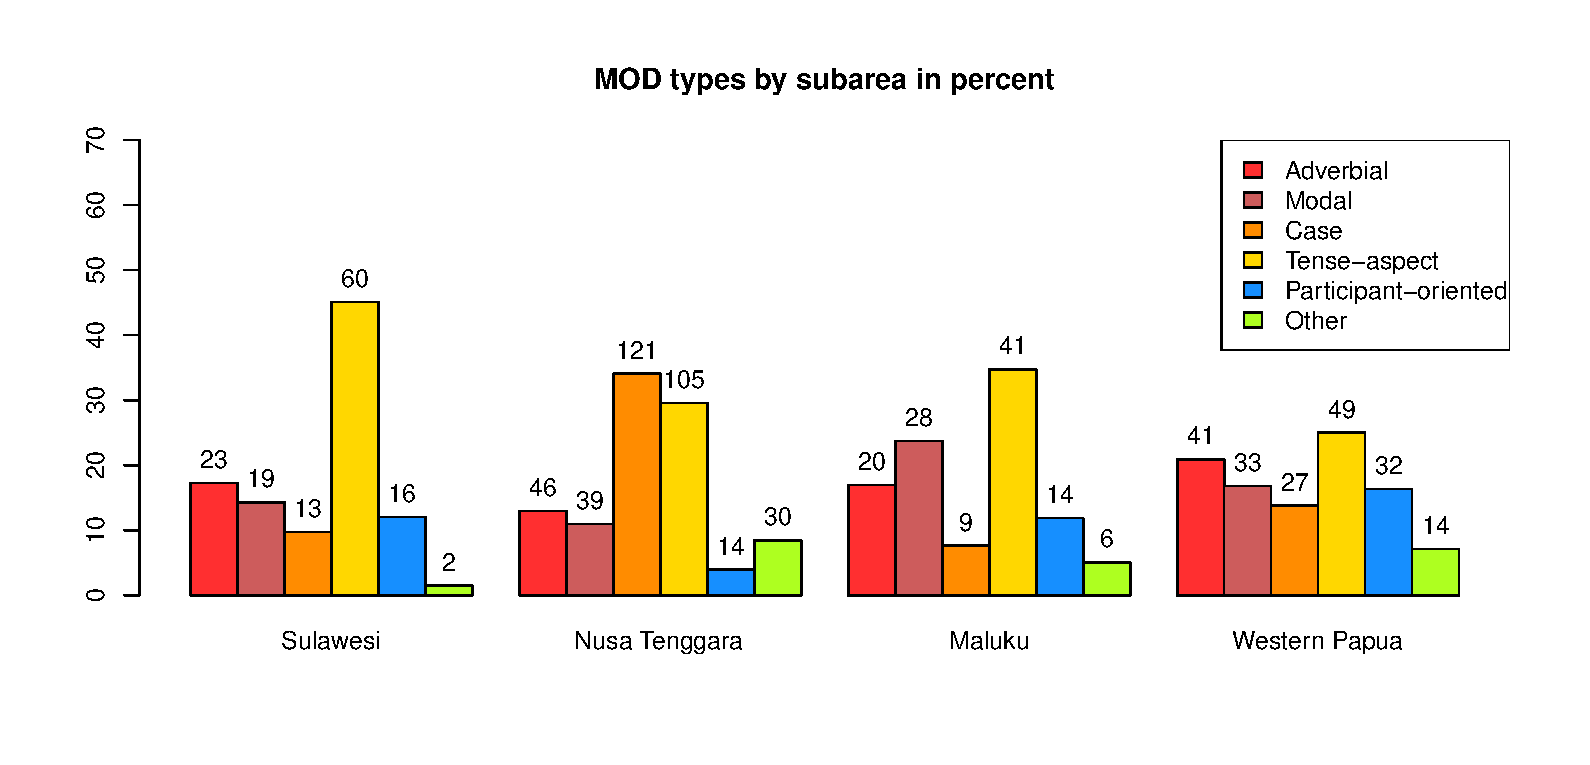
\includegraphics[width=\columnwidth]{../R/plots/MOD_Group.eps}
\caption[MOD types by subarea]{MOD types by subarea. Numbers on top of the bars refer to the number of observations in the dataset.}\label{fig:mod-group}
\end{figure}


Table \ref{table:MOD_language} below is a computation of \textsc{mod} construction numbers by language. As might be expected, a more fine-grained resolution of \textsc{mod} distribution across the dataset reveals further patterns. In the Sulawesi languages we again find the by now familiar division into northern Sulawesi languages (Pendau, Tajio), envisaging very little use of \textsc{mod} MVCs, and into the south-eastern languages for which \textsc{mod} use is clearly a pervasive phenomenon. Some other languages also deviate from the general picture by only using one of the functional groups, and in very small numbers. For Alorese (\textsc{nus} subarea) and Abun (\textsc{pap}) only adverbial constructions could be found. Dusner only contributes observations of case-marking constructions to the dataset. And finally, Sougb only has modal \textsc{mod} constructions, or so the numbers suggest.

\begin{table}
\centering

\begin{tabular}{lrrrrrr}
  \lsptoprule
  & \multicolumn{4}{c|}{event-oriented} & & \\
 & {adverbial} & {modal} & {case} & {tense-aspect} & {participant-oriented} & {other}\\ 
  \hline
  Muna &   6 &   3 &   2 &  12 &   8 &   1 \\ 
  Pendau &   0 &   1 &   0 &   3 &   1 &   0 \\ 
  Tajio &   5 &   0 &   0 &   1 &   0 &   0 \\ 
  Tolaki &   4 &   1 &   0 &  33 &   2 &   0 \\ 
  TukangBesi &   8 &  14 &  11 &  11 &   5 &   1 \\ \hline
  Abui &   3 &  14 &  30 &  15 &   3 &   8 \\ 
  Alorese &   4 &   0 &   0 &   0 &   0 &   0 \\ 
  Bunaq &  15 &   1 &   0 &  28 &   3 &   8 \\ 
  Kaera &   0 &   0 &   2 &   0 &   0 &   2 \\ 
  Kambera &   1 &   2 &  18 &   3 &   0 &   0 \\ 
  Klon &   6 &   8 &  16 &   9 &   0 &   1 \\ 
  Makalero &   5 &   5 &  28 &   4 &   1 &   5 \\ 
  Teiwa &   5 &   0 &   3 &   9 &   0 &   0 \\ 
  Tetun &   0 &   0 &  13 &  10 &   3 &   0 \\ 
  Waimaqa &   5 &   9 &   8 &  24 &   0 &   6 \\ 
  WesternPantar &   2 &   0 &   3 &   3 &   4 &   0 \\ \hline
  Buru &  12 &  11 &   0 &   9 &   1 &   0 \\ 
  Selaru &   2 &   7 &   5 &   0 &   2 &   1 \\ 
  Taba &   2 &   4 &   2 &  11 &   1 &   2 \\ 
  Tidore &   4 &   4 &   2 &   8 &   2 &   3 \\ 
  Tobelo &   0 &   2 &   0 &  13 &   8 &   0 \\ \hline
  Abun &   1 &   0 &   0 &   0 &   0 &   0 \\ 
  Biak &   5 &   7 &   0 &   2 &   2 &   0 \\ 
  Dusner &   0 &   0 &   9 &   0 &   0 &   0 \\ 
  Hatam &   0 &   0 &   0 &   1 &   5 &   0 \\ 
  Inanwatan &   0 &   0 &   0 &   1 &   0 &   3 \\ 
  Maybrat &   0 &   3 &  15 &   3 &   8 &   1 \\ 
  Mor &   1 &   1 &   0 &   3 &   2 &   0 \\ 
  Moskona &   8 &   1 &   0 &  13 &   7 &   9 \\ 
  Mpur &   1 &   5 &   1 &   2 &   7 &   0 \\ 
  Sougb &   0 &   3 &   0 &   0 &   0 &   0 \\ 
  Wooi &  25 &  13 &   2 &  24 &   1 &   1 \\ 
   \hline
   \end{tabular}
   \caption{Distribution of attested \textsc{mod} constructions across languages}
\label{table:MOD_language}

\end{table}


Turning to the morphosyntactic properties of \textsc{mod} constructions, we find a much more diverse picture than with component-relating constructions in the previous section. This is hardly surprising as the latter form a small set of uniform constructions that seem to exhibit little variation across EI. Modifying constructions, on the other hand, are a heterogeneous pool of constructions with similar functions that are strongly influenced by the respective source lexemes of the modifier verb, as well as the specific grammaticalisation cline. This leads to the picture illustrated by Table \ref{table:mod_formal} below. The numbers show that the majority of \textsc{mod} MVCs still conforms to the default \textsc{MVC} that became visible at the end of chapter \ref{ch:gram}: a construction with arguments tied together in `same subject' fashion, with inflection found on two verbs placed adjacent to each other. \textsc{mod} constructions as well are preferentially construed with the same subject pattern (the second most frequent argument configuration being event-to-argument reanalysis ``E"), a double-head marking is prevalent, and the verbs mostly appear in contiguous sequence. What is noticable, though, is that \textsc{mod} constructions do not exhibit the same amount of variation with respect to contiguity (the two most extreme values, ``3" and ``4" constituents intervening, are missing).

\begin{table}
\centering

\begin{tabular}{rrrrrrr}
  \lsptoprule
Referentiality & S & SO & D & A & E & X \\ 
  \hline
  adverbial &  74 &   2 &   6 &   0 &  48 &   0 \\ 
  modal &  95 &   0 &   0 &   1 &  16 &   7 \\ 
  case & 126 &   0 &  21 &   3 &  17 &   3 \\ 
  tense-aspect & 179 &   2 &   9 &   0 &  61 &   4 \\ 
  participant-oriented &  58 &   0 &  11 &   1 &   6 &   0 \\ 
  other &  27 &   0 &   4 &   0 &  20 &   1 \\ 
   \hline
 \\
  \hline
Headedness & B & 1 & 2 & S & N \\ 
  \hline
  adverbial &  35 &  18 &   0 &  13 &   6 \\ 
  modal &  57 &   2 &   8 &   3 &   1 \\ 
  case &  25 &  21 &   1 &  19 &   1 \\ 
  tense-aspect &  71 &  48 &   4 &   8 &  13 \\ 
  participant-oriented &  52 &   1 &   1 &   4 &   3 \\ 
  other &  11 &   6 &   3 &   1 &   1 \\ 
   \hline
 \\
  \hline
Contiguity & W & C & 1 & 2 \\ 
  \hline
  adverbial &   1 & 118 &  11 &   0 \\ 
  modal &   0 &  99 &  18 &   2 \\ 
  case &   0 & 127 &  43 &   0 \\ 
  tense-aspect &   4 & 220 &  27 &   4 \\ 
  participant-oriented &   0 &  58 &  16 &   2 \\ 
  other &   3 &  42 &   7 &   0 \\ 
   \hline
\end{tabular}
\caption[Morphosyntactic properties of \textsc{mod} constructions]{Morphosyntactic properties of \textsc{mod} constructions in EI. Table components from top to bottom refer to referentiality (see section §\ref{sec:argumentstructure}), headedness (see section §\ref{sec:headedness}), and contiguity (see section §\ref{sec:contiguity}), respectively.}
\label{table:mod_formal}

\end{table}


The following sections turn to the different functional groups introduced above, and provide examples from different constructions and subareas.

\subsection{Adverbial}\label{sec:adverbial}

Adverbial \textsc{mod} constructions cover two groups of modifier verbs that fulfill `adverbial functions'. Adverbial constructions proper contribute adverb-semantics that in non-serialising languages such as English are expressed by adjectives or adverbs. In this group of \textsc{mod} constructions, the modifying verb is recruited from a class of stative verbs. The second group, manner \textsc{mod}s, are made of what seem to be full-fledged verbs that are used in the modifier slot of the construction. As a heuristic, I assumed that such instances of \textsc{mod} constructions could be translated with the help of the phrase ``do X in Y manner", where X is the matrix verb, and Y refers to the semantics of the modifying verb. Table \ref{table:adverbial} presents the basic numbers. 

\begin{table}


\begin{tabular}{ll}
\lsptoprule
Feature&Value\tabularnewline
\hline
Template&V1 \textsc{matrix verb} * V2 \textsc{modifier verb}\tabularnewline
No. of attested instances& 130/2146 \tabularnewline
No. of attested languages& 23/32 \tabularnewline
Distribution across areas& \textsc{sul} (4/5), \textsc{nus} (9/11), \textsc{mal} (4/5) \textsc{pap} (6/11) \tabularnewline
Distribution across families& \textsc{pap} (10), \textsc{aus} (13) \tabularnewline
\hline
\end{tabular}
\caption[Template and basic distribution of adverbial \textsc{mod} MVCs]{Template and basic distribution of adverbial \textsc{mod} MVCs in the EI data set. The asterisk indicates that matrix verb and modifier verb may occur in both positions.}
\label{table:adverbial}
\end{table}


The percentages from Figure \ref{fig:mod-group} above seem to indicate that adverbial modification is most widespread in the Western Papua languages. As Table \ref{table:MOD_language} shows, however, most instances come from just one language, the corpus language Wooi, and in fact only 6 of 11 \textsc{pap} languages display multi-verbal adverbial constructions. Wooi has two constructions of adverbial MVCs. First, there is a small class of stative verbs that are able to take inflection, and appear close to the matrix verb they modify. This pattern is illustrated in example (\ref{wooi_37}) with the modifier of speed, \textit{mararu}. The example consists of two MVCs, a motion complex formed by \textit{vavu} and \textit{taveri}, and a modifying constructions where \textit{mararu} is added. Note that both the component-relating process as well as the modification by \textit{mararu} do not add further spatiotemporal stages to the event scheme. The third verb, \textit{taveri}, remains uninflected due to its deranked status within the motion complex, but would in other contexts inflect as well. As \textit{mararu} seems to modify the whole motion complex, I assume that the modifying construction forms only after the motion verbs merge their components. However, the exact scope of the modifier verb remains ambiguous in many examples (alternatively one might assume here that \textit{mararu} targets the matrix verb \textit{vavu}, and the whole modified motion construal is then specified by \textit{taveri}).

\ea \label{wooi_37}
%\begingl
%\rightcomment{{\small \textbf{Wooi} \textsc{pap}}}
\gll tamararu tambavu taveri \\
ta-mararu ta-vavu taveri \\
\glc 1\acs{pl}.\acs{in}-fast 1\acs{pl}.\acs{in}-return.home return \\
\glft `(and) we can go home fast.' \trailingcitation{{\small (HIVIAY\_exp)}}\\ 
\z
\xe

A second adverbial MVC pattern involves postverbs that do not normally appear without a matrix verb. These are always construed with a shared set of verbal affixes (which is not always visible if there is no resumptive object suffix attached to the postverb, such as \textit{-a} below). Example (\ref{wooi_30}) is a typical case.

\ea \label{wooi_30}
%\begingl
%\rightcomment{{\small \textbf{Wooi} \textsc{pap}}}
\gll tatong harata mara \\
ta-ong hara=a mara \\
\glc 1\acs{pl}.\acs{in}-use wrong=\acs{obj}.\acs{nsg} \acs{top} \\
\glft `if we use it wrongly' \trailingcitation{{\small (MANTERA\_magic\_charms)}}\\ 
\z
\xe

A number of EI languages derives such modifiers by way of reduplication, and they are mostly considered adverbs, not verbs proper. This is why examples like the following one from Kaera have been excluded from the corpus. Note, however, that in some languages `adverbial' modifiers are treated as verbs (by the respective authors) despite their reduplicated form, as in example (\ref{Bunaq17}) from Bunaq. The distribution of adverbial MVCs would thus be more widespread in EI if all instances of reduplicated modifiers were counted as verbs\footnote{Excluding all instances of reduplication on verbs would seem not helpful either as this would also pertain to dynamic verbs where reduplication in EI frequently produces Aktionsart differences, such as iterative or intensive readings.}.

\ea \label{}
%\begingl
%\rightcomment{{\small \textbf{Kaera} \textsc{nus}}}
\gll ging kali~kali ekeng \\
3\acs{pl} \acs{rdp}~slow climb.up \\
\glft `They climb up slowly.' \trailingcitation{{\small (Klamer 2014: 138)}}\\ 
\z
\xe
\ea \label{Bunaq17}
%\begingl
%\rightcomment{{\small \textbf{Bunaq} \textsc{nus}}}
\gll leleq enoq~enoq \\
flow slow~\acs{rdp} \\
\glft `(The water) runs really slowly.' \trailingcitation{{\small (Schapper 2009: 451)}}\\ 
\z
\xe

Manner constructions are formed by combining LLEs from two active verbs, most of them process verbs. The verbs that are in modifying function can also appear in simplex predicates elsewhere. Two major semantic fields may be distinguished. First, motion LLEs are modified by verbs denoting manner of motion, or otherwise compatible concepts that can be carried out during the motion process. Example (\ref{Bunaq_87}) from Bunaq illustrates such a case where the second verb provides information on the intention of the motion process (``in flight"). 

\ea \label{Bunaq_87}
%\begingl
%\rightcomment{{\small \textbf{Bunaq} \textsc{nus}}}
\gll Tebe tama sai, \textbf{borus} \textbf{ciwal} liol \\
return enter exit move.through flee continue \\
\glft `In turn (she) went in (then) out, continuing going through in flight.’ \trailingcitation{{\small (Schapper 2009: 472)}}\\ 
\z
\xe

Second, verbs of searching are quite often found in modifying function. The Biak case in (\ref{Biak_18}) shows such a construal, again together with a motion LLE, forming a motion PLE with manner specification. Verbs of searching are, however, also found accompanying non-motion verbs (for instance, \textsc{call} someone in a searching manner).

\ea \label{Biak_18}
%\begingl[glhangstyle=none]
%\rightcomment{{\small \textbf{Biak} \textsc{pap}}}
\gll Rofan anine \textbf{ifrar} \textbf{syéwaro} + romámkun anine \\
rofan an-i-ne i-frar s$<$y$>$éwar=o romá-mkun an-i-ne \\
\glc dog \acs{giv}-3\acs{sg}.\acs{spec}-this 3\acs{sg}-run $<$3\acs{sg}$>$seek=O child-little \acs{giv}-3\acs{sg}.\acs{spec}-this \\
\glft `This dog ran seeking for this child.' \trailingcitation{{\small (van den Heuvel 2006: 189)}}\\ 
\z
\xe

\subsection{Modal}\label{sec:modal}

Modal \textsc{mod} constructions convey a range of functions that are expressed in non-serialising languages by modal verbs, interrogative pronouns, permissives, evidential and hypothetical elements, among others. The functional common ground of all these is that the default factual mode of the utterance is modified, either in terms of agent-related properties (desiderative, abilitative, deontic),  with respect to event status (evidential, hypothetical, conative), or discourse-related (interrogative, hortative). The two latter functions are only rarely attested in the EI dataset for very few languages; the bulk of modal \textsc{mod} constructions refer to agent-related modification, that is desiderative, abilitative, and, to a lesser degree, deontic semantics. Table \ref{table:modal} summarizes the main facts about the distribution of \textsc{mod} constructions across EI, showing that the majority of EI languages utilise \textsc{mod} MVCs at least for some of the functions.

\begin{table}


\begin{tabular}{ll}
\lsptoprule
Feature&Value\tabularnewline
\hline
Template&V1 \textsc{matrix verb} * V2 \textsc{modifier verb}\tabularnewline
No. of attested instances& 119/2146 \tabularnewline
No. of attested languages& 22/32 \tabularnewline
Distribution across areas& \textsc{sul} (4/5), \textsc{nus} (6/11), \textsc{mal} (5/5) \textsc{pap} (7/11) \tabularnewline
Distribution across families& \textsc{pap} (11), \textsc{aus} (11) \tabularnewline
\hline
\end{tabular}
\caption[Template and basic distribution of modal \textsc{mod} MVCs]{Template and basic distribution of modal \textsc{mod} MVCs in the EI data set. The asterisk indicates that matrix verb and modifier verb may occur in both positions.}
\label{table:modal}
\end{table}


Two main groups may be distinguished: (i) constructions with pseudo-modals that resemble modal verb constructions (but do not show the usual distinctions in finiteness), and (ii) adverb- or pronoun-like elements that morphosyntactically behave like verbs (or are treated as such by the respective data sources). The following examples illustrate typical constructions from the first group. The pair of examples in (\ref{Taba_29}) and (\ref{Taba_30}) from Taba exemplify what I take to be a core property of \textsc{mod} constructions, at least in prototypical cases: that the modifying constituent has gained the status of an independent constituent under the grammaticalisation process, and may occur in different positions within the clause (if the respective language does not require absolutely rigid constituent order in the clause). In the Taba example, neither the principle of iconic ordering nor any other rigid constructional template constrains the use of \textit{ahan}. Although this freedom of ordering does not exist in many other instances of \textsc{mod} constructions, it could be predicted that \textsc{mod} constructions in different languages grammaticalising similar lexemes display differential ordering of matrix verb and modifier verb (depending on the source lexeme, and its original position). This variation sets \textsc{mod} constructions apart from component-relating and stage-relating constructions, which are always guided by general ordering principles.

\ea \label{Taba_29}
%\begingl
%\rightcomment{{\small \textbf{Taba} \textsc{mal}}}
\gll npe nahan \\
n=pe n=ahan \\
\glc 3\acs{sg}=do 3\acs{sg}=be.able \\
\glft `He can do it.' \trailingcitation{{\small (Bowden 2001: 316)}}\\ 
\z
\xe

\ea \label{Taba_30}
%\begingl
%\rightcomment{{\small \textbf{Taba} \textsc{mal}}}
\gll wwe nahan ncagal \\
wwe n=ahan n=sagal \\
\glc leg 3\acs{sg}=be.able 3\acs{sg}=step \\
\glft `my leg would be able to walk.' \trailingcitation{{\small (Bowden 2001: 316)}}\\ 
\z
\xe

The most frequent cases of pseudo-modals are desiderative constructions that express desire, want or intention of the actor to perfom the action contributed by the matrix verb. Here are two examples from different subareas. The first example in (\ref{Bunaq_2}) shows the only case in the dataset where the desiderative verb comes second and not first (despite the fact that Bunaq is an AVO language). Recall from section §\ref{sec:criteria_mvcs} that modifying constructions do not show constant behaviour in terms of operator placement. While TAM and person indexing operator values are typically shared across all verbal constituents in \textsc{mod} constructions, this is not true for negation, where at least in some \textsc{mod} constructions, negation of just one constituent seems possible. The Bunaq example in (\ref{Bunaq_2}) reflects this behaviour as the prospective marker \textit{gie} here only targets the motion constituent. This is in contrast to component-relating and stage-relating constructions in Bunaq where operators such as \textit{gie} need to have scope over the entire construction (cf. Schapper 2009: 443f.).

\ea \label{Bunaq_2}
%\begingl
%\rightcomment{{\small \textbf{Bunaq} \textsc{nus}}}
\gll baqi o mal gie heten \\
\acs{nprx}.\acs{an} \acs{foc}.\acs{add} go \acs{prosp} want \\
\glft `She also wants to walk.’ \trailingcitation{{\small (Schapper 2009: 444)}}\\ 
\z
\xe

Example (\ref{Wooi111}) from Wooi illustrates the order desiderative verb -- matrix verb. At least in Wooi, this order reflects  original source properties of the modifier verb. The origin of \textit{o} `want' is still transparent in Wooi: it is derived from \textit{oyo} `say' which is also frequently attested in a short form \textit{o} (\textit{o} `want', however, is always short, and never appears as \textit{oyo}). Thus desiderative constructions with \textit{o} originated from speech complement constructions where the sentential complement followed the \textsc{say} verb (and eventually got reanalysed as matrix verb constituent of a desiderative construction).

\ea \label{Wooi111}
%\begingl
%\rightcomment{{\small \textbf{Wooi} \textsc{pap}}}
\gll co vio to Nunoing vane \\
ti-o $<$i$>$vo to N. vane \\
\glc 3\acs{sg}-want $<$3\acs{sg}$>$row \acs{dir} N. \acs{det}.\acs{nprx} \\
\glft `(for example, if) he wants to go to Miosnum' \trailingcitation{{\small (HIVIAY\_exp)}}\\ 
\z
\xe

Speech act complementation can have a shift in subject arguments (for instance, in \textit{I say you do} type constructions). Given that speech act complementation is the source of at least some of the desiderative MVCs coded here as \textsc{mod}s, this raises the question whether desideratives of this sort can have the same shift in arguments. In English, want constructions are overtly biclausal, and involve raising of the dependent clause subject to the object of the matrix clause in case the `wisher' is not coreferential with the referent that is supposed to perform the action. Think of something like \textit{I want Jones to butter his toast at midnight} where, in structural terms, Jones belongs to the subordinate clause but is raised to object status. Such constructions are also possible in some EI languages with the only difference that there is no cue as to a biclausal construal. Consider an example from Selaru.

\ea \label{Selaru_4}
%\begingl[glhangstyle=none]
%\rightcomment{{\small \textbf{Selaru} \textsc{mal}}}
\gll Majelis-ke r-buma ta-wahuk + nur-Vre rahean.rahean \\
elders-\acs{art} 3\acs{pl}-want 1\acs{pl}.\acs{in}-gather coconut-\acs{pl} ten.by.ten \\
\glft `The church elders want us to gather coconuts in tens.‘ \trailingcitation{{\small (Coward 2005: 112)}}\\ 
\z
\xe

In Selaru both same-subject desiderative constructions, as well as ones without argument sharing, as in (\ref{Selaru_4}), are equally licit. Argument interaction in such examples has been coded ``X" as the exact argument relation between the constituents is not made transparent by morphosyntactic marking (note that such examples explain the conspicuous number of 7 ``X" cases for modal \textsc{mod} constructions in Table \ref{table:mod_formal} above). This is, however, not the case in all languages. Wooi is different in this regard. We might expect to find a conceptual overlap between speech act complements (I say he takes), and desiderative readings (I want him to take), but this is not supported by the Wooi data corpus. Each time there is a shift in subject indexing between \textsc{say}/\textsc{want} and matrix verb, the translation given indicates that the construction is still understood in its literal sense as a speech complement.\footnote{Note that the interrelatedness between cognitive verbs like \textsc{wish}, and speech verbs like \textsc{say} reflects the deeper cultural doctrine of the `opacity of other minds' that is well-developed in many languages from New Guinea and parts of Oceania. Opacity of the other mind describes what can be perceived as a cultural reluctance of stating directly what other people think or believe, as this is deemed impossible to know from an outside perspective. Instead of saying, for instance, \textit{Jones wants to eat toast at midnight}, one would rather resort to a behaviorist interpretation (Robbins 2008) like \textit{Jones says he eats toast at midnight}, thus circumventing a direct statement about Jones' inner feelings. See Robbins and Rumsey 2008, Robbins 2008, and Rumsey 2013 on the opacity of other minds.}

Turning to the second group of modal \textsc{mod} constructions, we find adverb or pronoun-like elements that take inflection and behave like a full-fledged verb. These \textsc{mod}s are rare in the dataset and basically confined to south-eastern Sulawesi and some odd examples from Papuan languages of the TAP area (Abui, Makalero). The following examples from Tukang Besi show an interrogative pronoun that is inflected like a verb in (\ref{Tukang_17}), and an evidential construction in (\ref{Tukang_18}). Comparable constructions are otherwise hardly found in the dataset.

\ea \label{Tukang_17}
%\begingl
%\rightcomment{{\small \textbf{Tukang Besi} \textsc{sul}}}
\gll \textbf{o-ha'a} tabeda \textbf{to-wila} loeloe? \\
3\acs{rls}-why necessary 1\acs{pl}.\acs{rls}-go slowly \\
\glft `Why will we have to go slowly?' \trailingcitation{{\small (Donohue 1999: 191)}}\\ 
\z
\xe

\ea \label{Tukang_18}
%\begingl
%\rightcomment{{\small \textbf{Tukang Besi} \textsc{sul}}}
\gll \textbf{o-tantu} \textbf{no-rato} sabentara \\
3\acs{rls}-certain 3\acs{rls}-arrive in.a.moment \\
\glft `They'll be here in a moment for certain.' (i.e., 'It is certain they will arrive in a moment') \trailingcitation{{\small (Donohue 1999: 189)}}\\ 
\z
\xe

\subsection{Case-marking} \label{sec:case-marking}

Case-marking is here understood in a non-strict sense: case-marking \textsc{mod} constructions comprise all those cases in which a (transitive) modifier verb introduces a further argument to the argument frame of the construction. This argument typically belongs to a set of oblique (adjunct) arguments, but some constructions seem to introduce core arguments as well. Attested arguments are direct object (patient, theme), experiencer, recipient, benefactive, comitative, instrumental, locative, source, and goal. Such MVCs have been identified in many serialising languages and can be considered one major group of prototypical SVCs according to many analyses (for instance Givon 1991, Aikhenvald 2006, Haspelmath 2016, see also \cite{lord1993historical} on the diachronic development of case-marking constructions in African languages). Table \ref{table:case} illustrates the basic facts on the distribution of case-marking MVCs across the EI area.

\begin{table}


\begin{tabular}{ll}
\lsptoprule
Feature&Value\tabularnewline
\hline
Template&V1 \textsc{matrix verb} * V2 \textsc{modifier verb}\tabularnewline
No. of attested instances& 170/2146 \tabularnewline
No. of attested languages& 18/32 \tabularnewline
Distribution across areas& \textsc{sul} (2/5), \textsc{nus} (9/11), \textsc{mal} (3/5) \textsc{pap} (4/11) \tabularnewline
Distribution across families& \textsc{pap} (9), \textsc{aus} (9) \tabularnewline
\hline
\end{tabular}
\caption[Template and basic distribution of case-marking \textsc{mod} MVCs]{Template and basic distribution of case-marking \textsc{mod} MVCs in the EI data set. The asterisk indicates that matrix verb and modifier verb may occur in both positions.}
\label{table:case}
\end{table}


As I have already noted above, case-marking MVCs can be considered a special feature of the Nusa Tenggara subarea as 121 from 170 instances are from \textsc{nus} languages. Nine of 11 Nusa Tenggara languages have such constructions, with Abui and Makalero being particularily productive in this regard.

Introduction of direct object arguments is only found in Makalero. The \textsc{take} verb \textit{mei} has developed into a light verb introducing arguments in case the main verb's object slot is already taken, for instance by a member of the large complement class (Huber 2011: 203f.). Verbal argument frames in Makalero may not exceed the number of two arguments. Therefore, when the object slot is in use, the addition of another argument slot is brought about by employing \textit{mei}. Examples (\ref{Makalero_56}), (\ref{Makalero_61}) and (\ref{Makalero_18}) illustrate three instances where the lightverb \textit{mei} is used. Each one adds a different kind of argument to the argument frame of the construction, making \textit{mei} a valency increaser with a broad range of functional context. In example (\ref{Makalero_56}), \textit{mei} introduces the object-theme \textit{Timor} because the ``complement-verb complex" (see Huber 2011: 131f.) consisting of matrix verb \textit{kini/ini} `do' and its complement \textit{lafu'} already constitute a saturated transitive argument frame. Note that Makalero has two kinds of linkers, \textit{=ini} and \textit{=isi}, both of which Huber analyses as clause linkers (2011: 457f.). Given, however, that at least \textit{=ini/ni} often appears in positions that obviously connect verbs of tightly bound constructions, I am assuming here that \textit{=ini/ni} rather provides a means to overtly extablish an integral construction rather than marking off two different clauses. Its use appears to be optional rather than required by the lightverb, as examples (\ref{Makalero_61}) and (\ref{Makalero_18}) are grammatical without a linker.

\ea \label{Makalero_56}
%\begingl[glhangstyle=none]
%\rightcomment{{\small \textbf{Makalero} \textsc{nus}}}
\gll negara taure’=ini tone’ ma’u=ni + Timor ere mei=ni lafu’-ini \\
nation which=\acs{ctr} perhaps come=\acs{lnk} T. 1\acs{dem} take=\acs{lnk} live-do:\acs{bd} \\
\glft '...whichever nation comes and rescues Timor...’ \trailingcitation{{\small (Huber 2011: 169)}}\\ 
\z
\xe

The next example in (\ref{Makalero_61}) shows the introduction of another theme-object. According to Huber's analysis, the object argument added by \textit{mei} is read as an instrument (2011: 204). This is indeed the case, but only at the level of the construction. It is the context rather than \textit{mei} by itself that invokes the instrument reading of the referent.

\ea \label{Makalero_61}
%\begingl
%\rightcomment{{\small \textbf{Makalero} \textsc{nus}}}
\gll Nana-uai aire’ sa’a-mei tina-ini? \\
elder.sibling-\acs{hon} now what:\acs{bd}-take cook-do:\acs{bd} \\
\glft ‘With what are you cooking?’ \trailingcitation{{\small (Huber 2011:204)}}\\ 
\z
\xe

Another use of \textit{mei} is in complex argument frames pertaining to construals of perception. In example (\ref{Makalero_18}) \textit{fi lolo-ini ere}, our language, is the stimulus of the perception event. It is first introduced by transitive \textit{mei}, and then, as I understand it, reintroduced as subject argument of an intransitive \textit{puna} `look'. So, literally, I would expect something along the lines of `our language, we take (it), it looks very bad'.

\ea \label{Makalero_18}
%\begingl[glhangstyle=none]
%\rightcomment{{\small \textbf{Makalero} \textsc{nus}}}
\gll po fi lolo-ini ere + fi=haka e’=ini mei puna hanu pa’u-pa’uk \\
\acs{adv} 1\acs{pl}.\acs{in} say-\acs{nm} 1\acs{dem} 1\acs{pl}.\acs{in}=\acs{ctrpres} \acs{dem}=\acs{lnk} take look very \acs{rdp}~bad \\
\glft ‘But our language, we see it as very bad...’ \trailingcitation{{\small (Huber 2011:189)}}\\ 
\z
\xe

Up to this point, the other EI languages have not contributed any examples. They only enter the picture when we turn to the introduction of adjunct arguments. Here we may distinguish two groups: (i) circumstantial arguments involve benefactives, comitatives and instruments; (ii) and local arguments comprise source, locative and goal arguments. Benefactive MVCs occur in four languages, Tukang Besi from the Sulawesi group, Makalero and Abui from Nusa Tenggara, and the language isolate Maybrat from the Bird's Head (Western Papua). I have already illustrated benefactive MVCs from these languages in section §\ref{sec:modification} on the semantics of modification.

Comitative and instrument constructions are more common throughout EI, but it is still only a minority of languages that have attested examples. Both groups of constructions may use a modifier verb that is glossed as 'with' (among other verbs that are specific to either constructional group, such as \textsc{accompany} verbs in comitative constructions). Maybrat even employs two different \textsc{with} verbs, one for each construction. Comitatives are attested for Tukang Besi, Abui, Western Pantar, Tetun Fehan, Waima'a, Teiwa, Selaru and Maybrat. The following pair of examples from Tetun again shows that at least some of the modifying MVCs allow the modifier consituent to be placed either before or after the matrix verb. At first glance the pattern seems identical as \textit{hó} `accompany' follows the directed motion verb \textit{bá} in each case. In example (\ref{Tetun_54}), however, the modifier verb is postponed after the matrix verb, while example (\ref{Tetun_57}) shows what I take to be a case of stacked MVCs: the modifying construction is nested into the action slot of a matrix motion-to-action MVC. Thus, the order \textit{bá} \textit{hó} looks just the same in both examples, but the directed motion verb in example (\ref{Tetun_57}) is in fact not part of the modifying construction. That is, in example (\ref{Tetun_57}) the modifier verb is preposed to its matrix verb \textit{k-adiuk}. This analysis is supported by van Klinken's own analysis (cf. 1999: 272): the comitative relation only holds true at the time of the playing, but not at the precursor motion phase.

\ea \label{Tetun_54}
%\begingl
%\rightcomment{{\small \textbf{Tetun} \textsc{nus}}}
\gll ha'u bá k-ó lós Am Bo'uk dei \\
1\acs{sg} go 1\acs{sg}-accompany just father Bo'uk only \\
\glft `I will go with only Am Bo'uk. (i.e. No-one else will go)' \trailingcitation{{\small (van Klinken 1999: 272)}}\\ 
\z
\xe

\ea \label{Tetun_57}
%\begingl
%\rightcomment{{\small \textbf{Tetun} \textsc{nus}}}
\gll ha k-bá \textbf{k-ó} feto sia \textbf{k-adiuk} \\
1\acs{sg} 1\acs{sg}-go 1\acs{sg}-accompany woman \acs{pl} 1\acs{sg}-play \\
\glft `[Every evening,] I go and play with (i.e. court) the girls' \trailingcitation{{\small (van Klinken 1999: 272)}}\\ 
\z
\xe

Note that \textit{hó} still appears to maintain a more concrete lexical meaning than, say, a verb that is only glossed as `with'. The next example is from Selaru, and shows such a case with a stripped-down comitative verb. Note again that comitative verbs may come either before or after the matrix verb, at least from a crosslinguistic perspective. This is in sharp contrast to what we find with both component-relating and stage-relating constructions.

\ea \label{}
%\begingl[glhangstyle=none]
%\rightcomment{{\small \textbf{Selaru} \textsc{mal}}}
\gll Y-aso sir ma r-al-a kotw ti + enen desike \textbf{y-or} amam desike \textbf{ra} ma ktei \\
3\acs{sg}-request them \acs{conj} 3\acs{pl}-give-Ø food \acs{conj} woman that(\acs{art}) 3\acs{sg}-with man that(\acs{art}) they.eat until done \\
\glft `He requested they give the food so that woman and that man [can] eat until done...' \trailingcitation{{\small (Coward 2007: 120)}}\\ 
\z
\xe

Instrumental MVCs are attested for Kambera, Klon, Tetun Fehan, Taba, Tidore, and Maybrat. In Kambera, instrumental MVCs are construed with a \textsc{use} verb, \textit{wàngu}. Here are three examples. In (\ref{Kambera_22a}), \textit{wàngu} is placed after the matrix verb, and this is the default position. In case the \textit{wàngu} VP is topicalised, it can precede the matrix verb, however, by changing its syntactic status through the use of a linker \textit{ba}, as example (\ref{Kambera_22b}) shows. Another possible manipulation of (\ref{Kambera_22a}) is focusing of the instrument argument licensed by \textit{wàngu}. Preposing \textit{huru}, the spoon, in example (\ref{Kambera_22c}) leaves the orginal order with a postposed \textit{wàngu} intact. One could argue that the Kambera case with \textit{wàngu} is just the same as the Makalero lightverb \textit{mei} in that both modifier verbs license a direct object argument. The reason for placing \textit{mei} in the direct object group above, and \textit{wàngu} in the instrumental argument group is that the former must have (at least originally) taken a theme object, while a \textsc{use} verb could arguably pass instrument semantics on to its object argument\footnote{Kambera \textit{wàngu} is in fact one of those generic verbs that are hard to pin down semantically. It may in simplex predicate contexts have the meaning `use', `do', `say' (and, derived from say, `want'; Klamer 1998: 284ff.). Therefore, placing the \textit{wàngu} construction in the group of instrumental MVCs heavily relies on the gloss `use'.}.

\pex 
\a \label{Kambera_22a}
%\begingl
%\rightcomment{{\small \textbf{Kambera} \textsc{nus}}}
\gll ku-taku uhu wàngu huru \\
1\acs{sg}.\acs{nom}-scoop rice use spoon \\
\glft `I scoop rice with a spoon' \\ 
\z
\a \label{Kambera_22b}
%\begingl
\gll wàngu huru ba ku-taku uhu \\
use spoon \acs{conj} 1\acs{sg}.\acs{nom}-scoop rice \\
\glft `With a spoon I scoop rice' \\ 
\z
\a \label{Kambera_22c}
%\begingl
\gll huru ku-taku uhu wàngu \\ 
spoon 1\acs{sg}.\acs{nom}-scoop rice use \\
\glft `I scoop rice with a SPOON' \trailingcitation{{\small (Klamer 1998: 287)}}\\ 
\z
\xe

The group of local case-marking construction, namely source, locative, and goal, is better attested than the other case-marking constructions. They are mainly formed by the use of a locative verb (mostly glossed as `be', `be.in', `be.at'). What is interesting is that the position of the locative verb often indicates its function by obeying the iconicity of order. That is, a preposed locative verb marks source arguments, a postposed locative verb may mark a goal. In Papuan head-final languages, however, the goal argument (with the locative verb) is usually placed before the matrix verb, indicating the somewhat grammaticalised nature of the modifier VP.

The first pair of examples in (\ref{Maybrat_60}) is from Maybrat, and illustrates a MVC introducing a source argument. Here, again, the order of both verbs seems interchangeable. Example (\ref{Abui_24}) is a source-marking construction from Abui. Locative verbs such as \textit{mi} are widespread across the TAP languages, and can express a range of different concepts, most of which are related to spatial semantics. When Abui \textit{mi} is construed with a motion verb, it marks the source or starting point of the motion process. Similar constructions can also be noticed in neighbouring languages, but sometimes a source NP is in fact lacking where it might be expected. Example (\ref{Klon_48}) illustrates such a case from Klon. It might be interpreted as covert source-marking: \textit{mi} adds a spatial starting point to the process of getting up, although no explicit mention is made of its exact location in the discourse space.

\pex \label{Maybrat_60}
\a
%\begingl
%\rightcomment{{\small \textbf{Maybrat} \textsc{pap}}}
\gll t-ama t-pat Sorong \\
1\acs{sg}-come 1\acs{sg}-from S. \\
\glft `I come from Sorong' \\ 
\z
\a
%\begingl
\gll ait y-pat rapuoh y-ama \\ 
3\acs{m} 3\acs{m}-from forest 3\acs{m}-come \\
\glft `He comes from the forest' \trailingcitation{{\small (Dol 2007: 206)}}\\ 
\z
\xe

\ea \label{Abui_24}
%\begingl
%\rightcomment{{\small \textbf{Abui} \textsc{nus}}}
\gll fala mi-a yaa! \\
house be.in-\acs{dur} go \\
\glft `go from the house!, lit. be in the house, go!’ \trailingcitation{{\small (Kratochvíl 2007: 356)}}\\ 
\z
\xe

\ea \label{Klon_48}
%\begingl
%\rightcomment{{\small \textbf{Klon} \textsc{nus}}}
\gll nang bo adob lega mi ihih \\
\acs{neg} \acs{seq} true 3\acs{sg}.\acs{top} be.at get.up \\
\glft `So he indeed got up' \trailingcitation{{\small (Baird 2008: 137)}}\\ 
\z
\xe

In Klon, modifier VPs with \textit{mi} can also occur postverbally, where they typically mark the endpoint or goal of a motion event. In example (\ref{Klon_99a}) below, we see that \textit{mi} may introduce local case NPs. Note that the NP \textit{alah} `house' is governed by \textit{mi}, and not by \textit{qad} `come'. The next example from Klon in (\ref{Klon_99b}) illustrates that the case interpretation of the NP licensed by \textit{mi} depends on the semantics of the matrix verb. The first instance is quite naturally interpreted as the endpoint of ego returning to the place called Hwak. The second \textit{mi}, however, combines with a stative verb and specifies the location of the sleeping.

\ea \label{Klon_99a}
%\begingl
%\rightcomment{{\small \textbf{Klon} \textsc{nus}}}
\gll kuur angkol a~awar qad alah mi ik \\
dog self \acs{rdp}~return come house be.at \acs{comp} \\
\glft `The dog itself came back and was at home' \trailingcitation{{\small (Baird 2008: 137)}}\\ 
\z
\xe

\ea \label{Klon_99b}
%\begingl[glhangstyle=none]
%\rightcomment{{\small \textbf{Klon} \textsc{nus}}}
\gll na lam gen u-elel, eben buur u-elel, + Hwak mi awar, Hwak weer mi taa' \\
1\acs{sg}.\acs{act} walk until \acs{vi}-search village flat \acs{vi}-search Hwak be.at return Hwak river be.at sleep \\
\glft `I walked until I found, found a flat village and returned to Hwak, slept at Hwak river' \trailingcitation{{\small (Baird 2008: 148)}}\\ 
\z
\xe

\subsection{Tense-Aspect}

The largest group of \textsc{mod} MVCs is formed by constructions that convey tense-aspect semantics (again understood here in a non-strict sense including Aktionsart concepts and all sorts of other temporal formatives), subsuming a wide range of different concepts. As in the modal group above, there are two sets of items that participate in such \textsc{mod} constructions. First, there is a large group of aspectual verbs that have been grammaticalised to different extents. And second, there is a much smaller group of adverb-like elements that behave like verbs and denote temporal concepts. The latter group is again more or less confined to the languages of south-eastern Sulawesi (Tolaki, Muna and Tukang Besi). Table \ref{table:tense-aspect} below presents the basic numbers of tense-aspect \textsc{mod} MVCs.

\begin{table}


\begin{tabular}{ll}
\lsptoprule
Feature&Value\tabularnewline
\hline
Template&V1 \textsc{matrix verb} * V2 \textsc{modifier verb}\tabularnewline
No. of attested instances& 255/2146 \tabularnewline
No. of attested languages& 26/32 \tabularnewline
Distribution across areas& \textsc{sul} (5/5), \textsc{nus} (9/11), \textsc{mal} (4/5) \textsc{pap} (8/11) \tabularnewline
Distribution across families& \textsc{pap} (13), \textsc{aus} (13) \tabularnewline
\hline
\end{tabular}
\caption[Template and basic distribution of tense-aspect \textsc{mod} MVCs]{Template and basic distribution of tense-aspect \textsc{mod} MVCs in the EI data set. The asterisk indicates that matrix verb and modifier verb may occur in both positions.}
\label{table:tense-aspect}
\end{table}


The group of aspectual verbs is dominated by \textsc{begin}, \textsc{finish} and \textsc{complete} verbs. I coded constructions that focus on modifying the telicity of event construals (that is, denoting their beginning or ending) as aspectual proper, and distinguished another group of constructions (basically also involving verbs of finishing) that show signs of grammaticalisation towards completive semantics (that is, denoting actions affecting the totality of participants). Iconicity seems to be a factor in the formation of such MVCs as \textsc{begin} verbs normally precede the matrix verb, and \textsc{finish} verbs follow it. The following examples give an illustration of how such aspectual \textsc{mod} constructions look like in EI. Example (\ref{Tolaki_38}) is from Tolaki, and makes use of the inflection pattern typical for that language: only the first verb takes inflection, which is in this case the modifier verb (this order is, as I mentioned above, an exception among the EI  languages, as \textsc{finish} verbs typically come last). The next example in (\ref{Western_14}) is from Western Pantar, and illustrates two intertwined MVCs. The dying is construed as the direct result of the slicing by means of a stage-relating MVC. To this bi-stage event schema, an aspectual \textsc{mod} MVC is added, reinforcing the endpoint of the dying. \textit{Gaata} here might either be interpreted as modifying \textit{hinna} alone, that is, the second event stage, or it might be read as modifying the whole event schema, that is, both stages. As the latter interpretation would clash with the conceptual event hierarchies, as proposed in chapter \ref{ch:sem}, I assume that in such cases, only the event stage adjacent to the modifier verb is modified (yielding something like slice -- [die finish]) (but see also §\ref{sec:clauselevelmodification}).

\ea \label{Tolaki_38}
%\begingl
%\rightcomment{{\small \textbf{Tolaki} \textsc{sul}}}
\gll ari 'aku-to \\
finish-1\acs{sg}.\acs{abs} $<$M$>$:\acs{apass}-eat \\
\glft `I've already eaten' \trailingcitation{{\small (Mead \& Youngman 2008: 123)}}\\ 
\z
\xe

\ea \label{Western_14}
%\begingl
%\rightcomment{{\small \textbf{Western Pantar} \textsc{nus}}}
\gll a-ule pai hinna kanna gaata \\
4\acs{sg} slice die finish already \\
\glft `They sliced his neck and killed him' \trailingcitation{{\small (Holton 2014: 82)}}\\ 
\z
\xe

Example (\ref{Buru_35}) from Buru illustrates the case of aspectual MVCs with a \textsc{begin} verb. In Buru and elsewhere, \textsc{begin} verbs precede their matrix verb, but the position of the pronominal subject is less rigid, and may shift to a position between the two verbs (see Grimes 1991: 215). The following example from Moskona exemplifies the use of a non-prototypical modifier verb. I have at several points made mention of motion verbs attaining aspectual semantics. In Moskona, it is obvious that \textit{eyja} still retains part of its motion semantics, but it may also be read as highlighting the beginning of an event. This relation between a stage-relating interpretation (go-build), and a modifying one (begin-build) sheds light on the diachronic pathways that exist between the different techniques of MVC formation. As constructions acquire new readings they may also acquire a different interpretation of their underlying event construal (for instance, by shifting from a bi-stage event schema to a mono-stage one).

\ea \label{Buru_35}
%\begingl
%\rightcomment{{\small \textbf{Buru} \textsc{mal}}}
\gll ringe peltanek iko boli fena-fena \\
3\acs{sg} begin go perimeter \acs{rdp}-village \\
\glft `He began to go around to each of the villages' \trailingcitation{{\small (Grimes 1991: 215)}}\\ 
\z
\xe

\ea \label{Moskona_48}
%\begingl[glhangstyle=none]
%\rightcomment{{\small \textbf{Moskona} \textsc{pap}}}
\gll edá, eri i-eyja i-or mod + jig merga or-i-em tas \\
then they.\acs{pl} 3\acs{pl}-go 3\acs{pl}-build house \acs{loc} wood \acs{num}:7-?-\acs{cst} again \\
\glft `Then, they began again to build a house in another tree.’ \\
or `they went again [and] built a house in another tree.’ \trailingcitation{{\small (Gravelle 2010:  297)}}\\ 
\z
\xe

Completives differ from \textsc{finish} semantics in that the endpoint of the event is not reached by some actor willfully ending it, but because a totality of referents is affected (see e.g. \cite{bybee1994evolution} for a diachronic assessment of completives). Not all EI authors distinguish between completives and \textsc{finish} semantics. The difference, however, stands out clearly when the glossing or translation of \textsc{finish} verbs involves some meaning of `all', as for instance in Waima'a \textit{maa}, or in the  \textit{kay} construction from Wooi. Waima'a \textit{Maa} is most often translated as `finish', but in some contexts the the translation and the glossing provided by the language consultant are markedly different, such as in example (\ref{wmh_x}) below. Here, \textit{maa} is glossed as `empty', indicating that the process of picking has ended because all the fruits had been picked. The completive semantics of \textit{maa} are also visible in examples such as (\ref{wmh_y}) where a wedding party prepares different kinds of items for the ceremony, and brings these items to the wedding place. \textit{Maa} in this context clearly does not refer to the endpoint of the bringing, but specifies the object of the bringing to include all items mentioned in the previous utterances. Completive MVCs such as these have been recorded in the EI dataset for a couple of languages in the Nusa Tenggara, Maluku, and Western Papua groups, but not for any of the Sulawesi languages.

\ea \label{wmh_x}
%\begingl
%\rightcomment{{\small \textbf{Waima'a} \textsc{nus}}}
\gll ne la kai oo ta ne uhu ma'a ulo \\
3\acs{sg} \acs{loc} wood above \acs{dist} 3\acs{sg} pick empty already \\
\glft `after the one at the top of the tree is done with picking (fruit)' \trailingcitation{{\small (pear\_Santina 025)}}\\ 
\z
\xe

\ea \label{wmh_y}
%\begingl
%\rightcomment{{\small \textbf{Waima'a} \textsc{nus}}}
\gll sire ani ma'a  ruo \\
3\acs{pl} bring all with \\
\glft `they bring it all' \trailingcitation{{\small (dom2\_kaben 138)}}\\ 
\z
\xe

What is found in the south-eastern Sulawesi area and its vicinity instead is tense-aspect MVCs of the second group introduced above, namely MVCs that are formed by stative non-prototypical verbs. Instances of these group cluster in their constructional make-up with modal \textsc{mod}s as already discussed in section §\ref{sec:modal} above. Here are three examples, each illustrating habitual modification by using a \textsc{mod} MVC. Although the languages use different head-marking strategies (first verb inflected in Tolaki versus all verbs inflected in same subject-manner in Muna and Tukang Besi), the overall constructional make-up is rather similar: the modifier verb comes first and is immediately followed by the matrix verb(s). Both Muna and Tukang Besi show what van den Berg (1989) referred to as ``subject harmonisation", that is, the modifier verb takes the same subject indexer as the matrix verb(s). As the example from Muna in (\ref{Muna_30}) further illustrates, more than one modifier verb may combine with a single matrix verb.

\ea \label{Tolaki_39}
%\begingl[glhangstyle=none]
%\rightcomment{{\small \textbf{Tolaki} \textsc{sul}}}
\gll a-no \textbf{ndee} \textbf{modea-'iro} + mbe-maroa i aahua-no \\
and-3\acs{sg}.\acs{nom} habitually $<$M$>$:hear-3\acs{pl}.\acs{abs} \acs{coll}-be.noisy at well-3\acs{sg}.\acs{gen} \\
\glft * and he usually heard them all being noisy at his well.' \trailingcitation{{\small (Mead and Youngman 2008: 123)}}\\ 
\z
\xe

\ea \label{Tukang_62}
%\begingl[glhangstyle=none]
%\rightcomment{{\small \textbf{Tukang Besi} \textsc{sul}}}
\gll te Wanse, \textbf{o-monea} \textbf{na-po-daga} + \textbf{na-para-aso}, no-karajaa, a mo'ane, wowine \\
\textsc{core} Wanci 3\acs{rls}-usual 3\acs{irr}-\acs{recip}-trade 3\acs{rls}-\acs{iter}-sell 3\acs{rls}-work \acs{nom} man woman \\
\glft `On Wanci, normally both men and women trade, and sell things, and work' \trailingcitation{{\small (Donohue 1999: 510)}}\\ 
\z
\xe

\ea \label{Muna_30}
%\begingl
%\rightcomment{{\small \textbf{Muna} \textsc{sul}}}
\gll ao-nea ae-rimba a-kala \\
1\acs{sg}.\acs{rls}-usual 1\acs{sg}.\acs{rls}-fast 1\acs{sg}.\acs{rls}-go \\
\glft `Usually I walk fast' \trailingcitation{{\small (van den Berg 1989: 238)}}\\ 
\z
\xe


\subsection{Participant-oriented}

The last four sections have dealt with modifying MVCs that target the event schema of a matrix verb, and add specific semantic content to it. I now turn to another group of \textsc{mod} MVCs that do not directly modify the event, but one of the participants that are associated with it. Participant-oriented MVCs are less frequent in the EI dataset, with 76 cases attested. Table \ref{table:participant} shows that only few instances are found across the Nusa Tenggara languages.

\begin{table}


\begin{tabular}{ll}
\lsptoprule
Feature&Value\tabularnewline
\hline
Template&V1 \textsc{matrix verb} * V2 \textsc{modifier verb}\tabularnewline
No. of attested instances& 76/2146 \tabularnewline
No. of attested languages& 21/32 \tabularnewline
Distribution across areas& \textsc{sul} (4/5), \textsc{nus} (5/11), \textsc{mal} (5/5) \textsc{pap} (7/11) \tabularnewline
Distribution across families& \textsc{pap} (10), \textsc{aus} (11) \tabularnewline
\hline
\end{tabular}
\caption[Template and basic distribution of case-marking \textsc{mod} MVCs]{Template and basic distribution of case-marking \textsc{mod} MVCs in the EI data set. The asterisk indicates that matrix verb and modifier verb may occur in both positions.}
\label{table:participant}
\end{table}


Two functions are prototypically expressed by participant-oriented MVCs: the first and foremost group of constructions specifies the number or the referential state of a referent. To this end, verboids with glosses such as `many', `all', `self', or `\textsc{number}' are combined with a matrix verb. This functional group is attested from south-eastern Sulawesi, but not in the north, across the Nusa Tenggara languages (Western Pantar, Abui, Bunaq), in the Maluku area (Tidore, Tobelo), and into Western Papua (Biak, Wooi, Mor, Moskona, Maybrat). Consider the following examples. In (\ref{Tukang_37}) from Tukang Besi, we can see a shared affix set enclosing both the matrix verb in V$_1$ and the numeral verb in V$_2$. The behaviour of the object suffix is exceptional in that, first, it has to be there, and, second, it has to agree in person and number with the subject prefix. A third restriction pertains to object expression in case the matrix verb is transitive. As the example pair illustrates, only unspecified (deleted) objects are permitted. Overt nominals, occurring either as a noun phrase or a verbal affix, render the construction ungrammatical.

\pex \label{Tukang_37}
\a
%\begingl
%\rightcomment{{\small \textbf{Tukang Besi} \textsc{sul}}}
\gll to-manga-nono'o-ngkita \\
1\acs{pl}.\acs{rls}-eat-be.six-1\acs{pl}.\acs{obj} \\
\glft `Six of us ate.' \\ 
\z
\a
%\begingl
\gll *to-manga-non'o-ngkita te mandara \\ 
1\acs{pl}.\acs{rls}eat-be.six-1\acs{pl}.\acs{obj} \textsc{core} sweet.potato \\
\glft  \trailingcitation{{\small (Donohue 1999: 197)}}\\ 
\z
\xe

Tobelo numeral verbs convey the same function as the numeral verboids in Tukang Besi, but appear in preverbal position. Example (\ref{Tobelo_39}) below illustrates that \textit{ruange} `three' behaves just like a full-fledged active verb with a subject indexer (statives would receive the double indexing introduced in section §\ref{sec:maluku}). The whole utterance consists of four verbs chained together, making up a total of three multi-verb relations discernible: the matrix construction is headed \textit{kagaro} `decide', which takes as a sentential complement the two following verbs. These verbs together form what I analyse as a stage-relating MVC of the motion-to-action type. Finally, the modifier verb \textit{ruange} is preposed to the complement-taking matrix verb \textit{kagaro}. As in the preceding examples, \textit{ruange} does not alter the event schema as such, but modifies the subject participant. Another construction that pertains to participant number involves a verboid glossed as `alone'. In example (\ref{Tobelo_29}) from Tobelo, \textit{tengo} is used in an existential construction with \textit{naga} `exist'. As a comparison with the appended text sources in Holton (2003) shows, \textit{tengo} may also function as a simplex predicate. In example (\ref{Tobelo_29}) it occupies a modifier slot, specifying that the woman introduced was acting all on her own. 

\ea \label{Tobelo_39}
%\begingl[glhangstyle=none]
%\rightcomment{{\small \textbf{Tobelo} \textsc{mal}}}
\gll jadi  ngomi mi-ruange mi-ma-hi-kagaro + mi-oiki mi-lye o-lyoku-iha \\
thus 1\acs{ex} 1\acs{ex}-three 1\acs{ex}-\acs{refl}-\acs{caus}-decide 1\acs{ex}-go 1\acs{ex}-get \acs{nm}-mountain-\textsc{land} \\
\glft `So we three decided to go to the mountains to get some' \trailingcitation{{\small (Holton 2003: 71)}}\\ 
\z
\xe

\ea \label{Tobelo_29}
%\begingl[glhangstyle=none]
%\rightcomment{{\small \textbf{Tobelo} \textsc{mal}}}
\gll naga a-nyawa mo-ma-tengo + mo-oiki ami-dumule-ika \\
exist \acs{nm}-person 3\acs{f}-\acs{refl}-alone 3\acs{f}-go 3\acs{f}.\acs{poss}-garden-\acs{all} \\
\glft `There was a woman who went to her garden.' \trailingcitation{{\small (Holton 2003: 66)}}\\ 
\z
\xe

This example is also a good illustration of another group of participant-oriented MVCs: the last two verbs in the utterance constitute what Holton calls a paratactic relative clause. It is the person introduced by the existential construction that acts as the subject of the motion event. Paratactic relativisation is comparatively rare in the EI dataset, and mostly occurs in Sulawesi languages (Tolaki, Muna, and Pendau). As they appear to modify participants rather than align events (answering the question \textit{what did participant X?} instead of \textit{what happened?}), I tentatively placed them with the participant-oriented \textsc{mod} MVCs, although a more in-depth analysis might probably find that they have a biclausal syntax, and should be included in the family of free juxtaposition MVCs. Still, what seems to set these constructions apart from \textsc{fjux} constructions is that they appear to be more closely integrated than typical \textsc{fjux} constructions, and that they obviously need to share the pivot argument to be relativised. The fact that paratactic relativisation constructions predicate over one of the participants governed by the matrix verb is reminiscent of depictive secondary predicates.

Depictive modification is the second frequent \textsc{mod} function in EI that can be associated with participants rather than with events. Depictives, or depictive secondary predicates in full, have been defined as predicating elements that operate over one of the participants selected by a matrix verb. The matrix verb at the same time constitutes the `primary' predicate of the clause (see e.g. \cite{schultze2004depictive} for definition and a crosslinguistic overview). The focus on participants rather than on predicates sets depictives apart from adverbial modification. Consider the two sentences \textit{Jones ate his toast fast} and \textit{Jones ate his toast hot}: in both sentences, we find a modifier in clause-final position modifying part of what is said. However, while \textit{fast} modifies the eating, that is, targets the event argument, \textit{hot} in the second sentence modifies the toast, that is, targets one of the participants associated with the event. A key property of such depictive predicates is that their time frame is bound by the time frame of the primary predicate. This would mean that in our example, the toast is hot only at the time of Jones eating it (as opposed to the temporal properties of attributive modifiers, as in \textit{Jones ate hot toast}).

As we have seen in section §\ref{sec:adverbial}, there is adverbial modification in EI languages that is expressed by MVCs. The same appears to hold true for depictives, although cases of depictive MVCs are less frequent, and their detection strongly depends on how much scrutiny the respective researcher puts into making this distinction in his or her data annotation. Here are some examples from different EI subareas. Example (\ref{Tidore_62}) from Tidore consists of two MVCs, a motion-to-action construction \textit{tagi pana}, and a modifying construction \textit{tulu soha}. As van Staden's translation illustrates, \textit{soha} `hungry' is here interpreted as modifying the subject participant rather than indicating the manner in which the resting takes place (`resting hungrily'). Note that the first MVC is here again interpreted as some kind of paratactic relativisation. The example pair in (\ref{Hatam_43}) shows a comparable construal from Hatam. Reesink suggests that \textit{nggum} 'hungry' could be interpreted as an adverbial modifier of V$_1$, as such sequences do not accept the insertion of a conjunction \textit{ba} `and'. In Bunaq, the position of the modifier verb indicates whether it has scope over a participant (preposed), or over the event argument (postposed). This is illustrated in the example pair (\ref{Bunaq_12}). As being naked is conceptually hard to interpret as the manner in which the motion event takes place, the second utterance is semantically odd.

\ea \label{Tidore_62}
%\begingl
%\rightcomment{{\small \textbf{Tidore} \textsc{mal}}}
\gll ngofa nde tagi pana namo tulu soha \\
child 3\acs{nhum}.here go shoot bird rest hungry \\
\glft `the child who had gone shooting birds rested (and) he was hungry' \trailingcitation{{\small (van Staden 2000: 279)}}\\ 
\z
\xe

\pex \label{Hatam_43}
\a
%\begingl
%\rightcomment{{\small \textbf{Hatam} \textsc{pap}}}
\gll ni-hara ni-nggum... \\
1\acs{ex}-ask 1\acs{ex}-hungry \\
\glft `we ask (because) we are hungry...' \\ 
\z
\a
%\begingl
\gll *ni-hara ba ni-nggum \\ 
\glft  \trailingcitation{{\small (Reesink 1999: 107)}}\\ 
\z
\xe

\pex \label{Bunaq_12}
\a
%\begingl
%\rightcomment{{\small \textbf{Bunaq} \textsc{nus}}}
\gll baqi omal he \\
\acs{nprx}.\acs{an} naked run \\
\glft `She ran naked' \\ 
\z
\a
%\begingl
\gll baqi he omal \\ 
\acs{nprx}.\acs{an} run naked \\
\glft `She ran nakedly' \trailingcitation{{\small (Schapper 2009: 449)}}\\ 
\z
\xe

\subsection{Other}

The previous sections presented examples of \textsc{mod} constructions that can be sorted into functional categories. While adverbial, modal, case-marking and tense-aspect MVCs operate over event construals provided by the respective matrix verb(s), participant-oriented \textsc{mod}s complement the event schema of the construction with further (predicative) information on one of the participants. This leaves us with a handful of cases, for which it is more difficult to assign a functional label. A look back at Table \ref{table:MOD_language} shows that the attested cases are not evenly distributed over the EI languages, but that they accumulate in some languages, such as Abui (8 cases), Bunaq (8 cases), Makalero (5 cases), or Moskona (9 cases). This is in part predictable because it is these languages that show the most pervasive use of MVCs throughout the EI area (in particular, the Nusa Tenggara languages). Another reason is that the grammatical notion of degree in comparisons is expressed in these languages through MVCs. Moskona is a good example, as its system of degree semantics is organised by verbal modifiers. Intensifiers, such as \textit{etew} in the Moskona example (\ref{Moskona_75}) below, are often analysed as verbs in EI languages. If one follows those analyses, the respective constructions would then form a modifying MVC. Comparative or superlative constructions involving the use of a verb like \textsc{exceed} are attested from other language families (see e.g. Aikhenvald 2006), but they appear to be scarce in the EI area. Example (\ref{Moskona_78}) illustrates such a case from Moskona.

\ea \label{Moskona_75}
%\begingl
%\rightcomment{{\small \textbf{Moskona} \textsc{pap}}}
\gll Eri i-em-en maeken(a) etew éra \\
they.\acs{pl} 3\acs{pl}-do garden be.much \acs{neg} \\
\glft `They don’t work in the garden a lot.’ \trailingcitation{{\small (Gravelle 2010: 303)}}\\ 
\z
\xe

\ea \label{Moskona_78}
%\begingl[glhangstyle=none]
%\rightcomment{{\small \textbf{Moskona} \textsc{pap}}}
\gll Ej-efer no-ma-i, + ofon efega oyf-omof ekris \\
female-child \acs{det}-far-\acs{giv} 3\acs{pl}.\acs{poss} body good-\acs{rdp} exceed \\
\glft `The young woman, her body(figure) is best.' \trailingcitation{{\small (Gravelle 2010: 304)}}\\ 
\z
\xe

Apart from degree functions, there are no constructions in this group that seem to have a wider distribution across EI. Take as an example the `narrow focus' construction that has only been described for Abui (Kratochvíl 2007: 385f.), but is not attested in any other EI language. The following pair of examples demonstrates the difference between a narrow focus MVC, and a construction made up of two juxtaposed VPs. The modifier verb is \textit{do} `hold, get', and must stand in preverbal position in order to impose the narrow focus reading on the matrix constituent.

\pex \label{Abui_99}
\a
%\begingl
%\rightcomment{{\small \textbf{Abui} \textsc{nus}}}
\gll e-do taa, ne-do na-rui-da \\
2\acs{sg}.\acs{loc}-hold lie 1\acs{sg}.\acs{loc}-hold 1\acs{sg}.\acs{pat}-erect-hold \\
\glft `As for you, sleep, as for me, I get up’ \\ 
\z
\a
%\begingl
\gll a taa, na=ng na-rui-da \\ 
2\acs{sg} lie 1\acs{sg}=see 1\acs{sg}.\acs{pat}-erect-hold \\
\glft `You sleep, I get up’ \trailingcitation{{\small (Kratochvíl 2007: 389)}}\\ 
\z
\xe

\section{Stage-relating constructions}\label{sec:stage-relating}

In the previous sections of this chapter, we dealt with MVCs that form on the level of the PLE, entailing only one underlying event stage (that is, the event arguments of all participating verbs must spatio-temporally coincide). Both component-relating constructions and modifying constructions arguably have Bohnemeyer and colleagues's macro-event property, as temporal modification is only possible at the level of the construction, but not at a lower level. Stage-relating constructions are different because neither do the LLEs merge their conceptual structure, nor does one LLE modify the other. Rather the LLEs are combined to form a two-stage event schema. This renders stage-relating MVCs intermediate between one-stage construction types like the aforementioned ones on the one hand, and free event-combining construals on the other (that I refer to as free juxtaposition). With the latter, stage-relating constructions share a complex spatio-temporal structure as each verb contributes its own event argument. Stage-relating constructions differ from free juxtaposition in that their construal is typically more condensed, and that there are clear constructional templates recognisable that reappear throughout most of the EI languages.

These constructional templates give rise to certain rather small verb classes. Only members of these classes are permitted to occupy the defining slot of stage-relating constructions. This defining slot normally comes first. From the body of the EI data, we may identify three broad functional groups. First, there is a group of \textsc{srel} constructions denoting orientation in the discourse landscape. Motion-to-action \textsc{srel}s are by now familiar as they have been illustrated by many examples. Their primary function is to denote a change in location of some acting participant, paired with a clear intention of performing some action at the place of destination. Position-action is similar to motion-to-action in that the action carried out by the actor is accompanied by details on the spatiotemporal setting. The only difference is that in construals of position-action MVCs, both event arguments are interpreted to overlap in space and time. The third construction that is part of the functional group of \textsc{srel}s pertaining to spatial orientation is action-to-position. With this construction, the position slot comes last, and specifies the spatial properties of an object that has been manipulated by some previous action. 

Second, there are at least two constructions that focus on manual action. Both constructions have a defining class of handling verbs. In handling-to-action, a verb of handling is minimally followed by an action verb, and sometimes the template also comprises a motion verb in intermediate position. Handling-to-placement may constitute a subgroup of handling-to-action, but are treated here as a different template, because the construction seems to fulfill the specific function of facilitating ditransitive construals of object relocation.

Third, there are three constructions all pertaining to causation. Cause-result combines a transitive verb of object manipulation with a transitive or, more often, intransitive verb denoting its result. In cases where the second verb is a stative verb that denotes a resultant state, I placed the respective cases under the label resultative construction. Still another related construction is the causative construction with a generic causative verb in first position. Such construals, I propose, still project a two-stage event schema as both verbs still contribute a full-fledged event argument. Yet the difference is that the semantics of the first event stage is not made explicit anymore. Table \ref{table:SREL_overview} illustrates the basic counts from the dataset.

\begin{table}


\begin{tabular}{lrrrrrrrr}
  \lsptoprule
&\multicolumn{3}{c|}{orientation} & \multicolumn{2}{c|}{handling} & \multicolumn{3}{c}{causation} \\
 & {motion-to-action} & {position-action} & {action-to-position} & {handling-to-action} & {handling-to-placement} & {cause-result} & {resultative} & {causative} \\  
  \hline
  Austronesian & 204 & 22 & 18 & 17 & 8 & 31 & 19 & 13 \tabularnewline
  Papuan & 128 & 20 &  6 &  49 & 22 & 12 & 14 & 22 \tabularnewline
   \hline
  Sulawesi & 67 & 1 & 1 & 0 & 0 & 1 & 5 & 0 \tabularnewline
  Nusa Tenggara & 78 & 14 & 16 & 24 & 25 & 14 & 6 & 19 \tabularnewline
  Maluku & 46 & 1 & 1 & 11 & 0 & 8 & 3 & 2 \tabularnewline 
  Western Papua & 141 & 26 & 6 & 31 & 5 & 20 & 19 & 14 \tabularnewline 
\lsptoprule
Total & 332 & 42 & 24 & 66 & 30 & 43 & 33 & 35 \tabularnewline
\hline
\end{tabular}
\caption[Distribution of \textsc{srel} types across EI]{Distribution of \textsc{crel} types across EI. Note that both subcalculations, i.e. into language family affiliation as well as into areal subgroups, each amount to the total number of observations given in the last row.}
\label{table:SREL_overview}


\end{table}


Turning to the distribution of \textsc{srel} MVCs across the EI area, we can see from Table \ref{table:SREL_overview} that motion-to-action is indeed the prototypical \textsc{srel} construction with a total of 332 recorded instances. All other \textsc{srel}s clearly lag behind: handling-to-action constructions are the secondmost widespread \textsc{srel} MVCs (N=66), followed by cause-result (N=43) and position-action (N=42). The others seem to constitute minor construals. Although motion-to-action is frequently found among all language groups, Figures \ref{fig:srel-family} and \ref{fig:srel-group} indicate small distributional differences. Both in the Papuan languages, as well as in the \textsc{nus} subarea, motion-to-action is attested less often in comparison to the other \textsc{srel} constructions (in both cases hardly reaching 50\%). This could suggest that \textsc{srel} diversity is higher in these groups. The secondmost frequent construction, handling-to-action, is more prevalent in Papuan languages (17.95\%) than in Austronesian languages (5.12\%). Its occurrence is geographically associated with the three subareas Nusa Tenggara, Maluku and Western Papua. Sulawesi languages do not show attested cases. Cause-result construals, on the other hand, seem to be more predominant in Austronesian languages (9.34\%) than in Papuan languages (4.4\%).

\begin{figure}[ht]
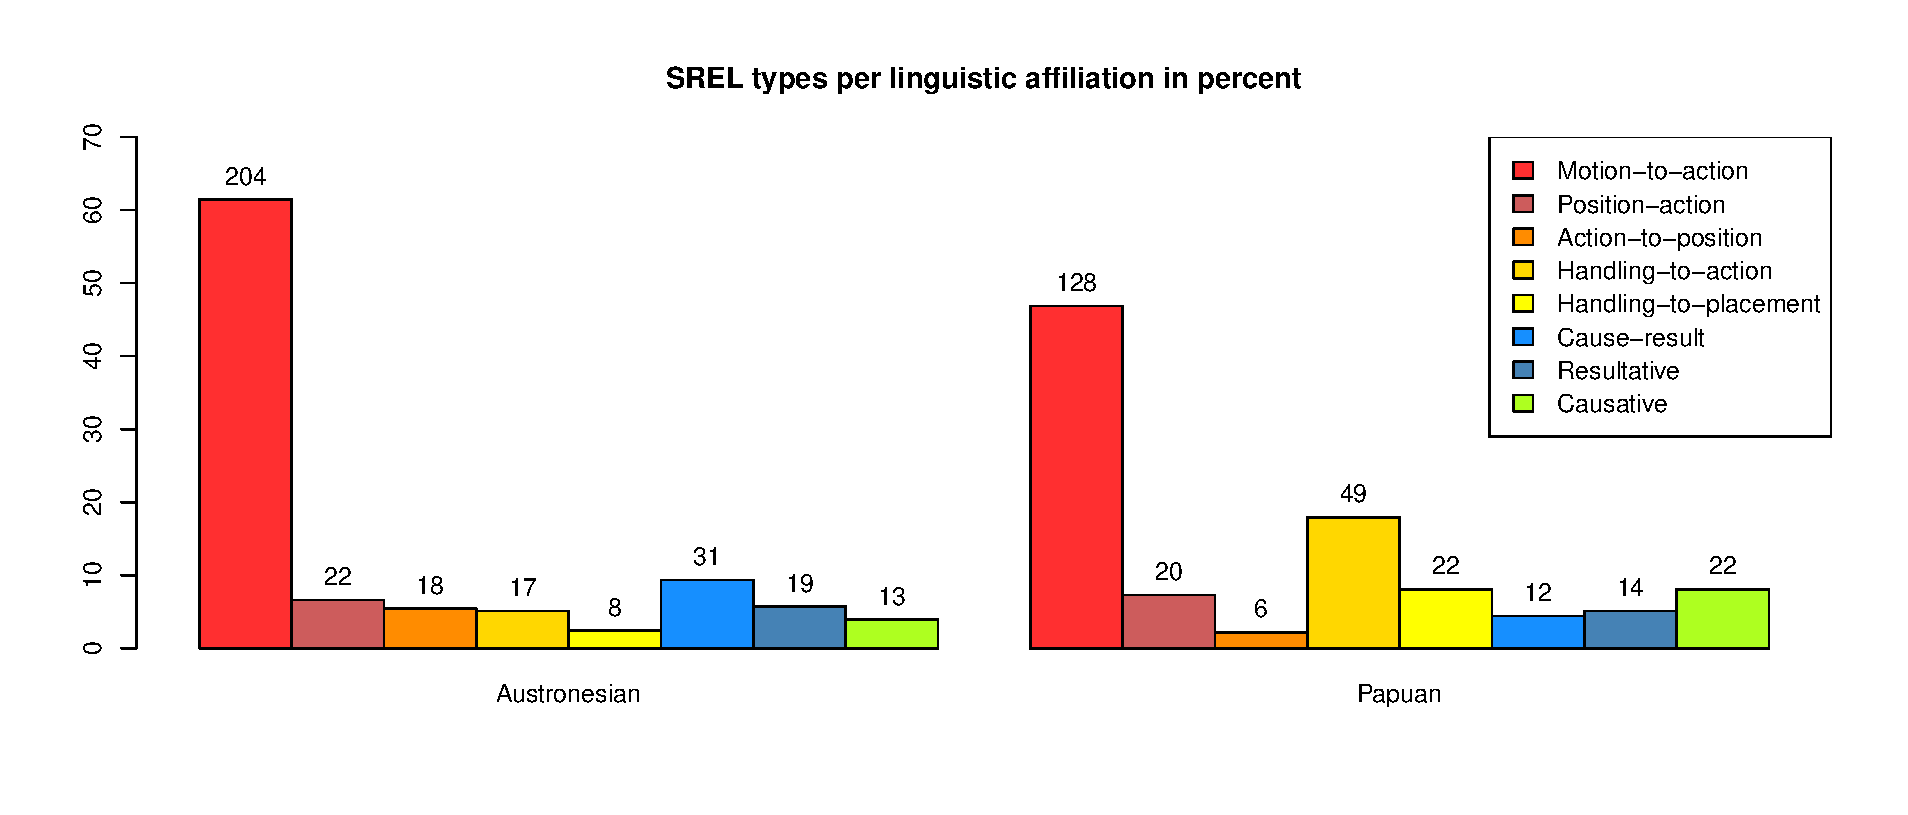
\includegraphics[width=\columnwidth]{../R/plots/SREL_Family.eps}
\caption[SREL types per linguistic affiliation in percent]{SREL types per linguistic affiliation in percent. Numbers on top of the bars refer to the number of observations in the dataset.}\label{fig:srel-family}
\end{figure}
\begin{figure}[ht]
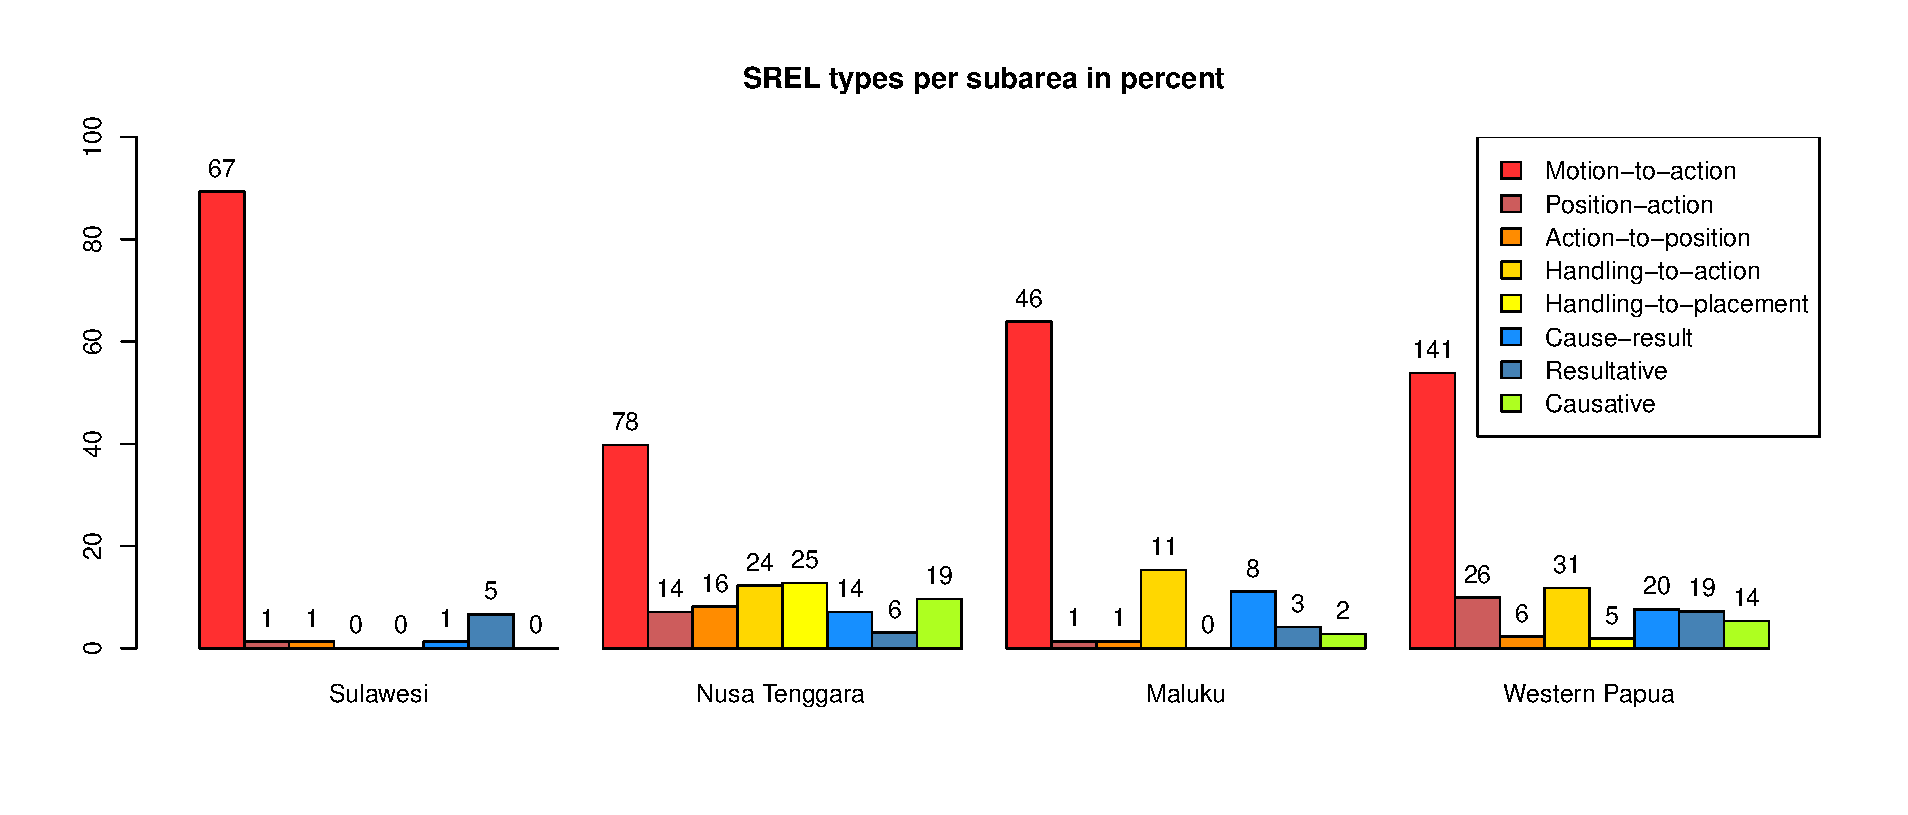
\includegraphics[width=\columnwidth]{../R/plots/SREL_Group.eps}
\caption[SREL types per subarea in percent]{SREL types per subarea in percent. Numbers on top of the bars refer to the number of observations in the dataset.}\label{fig:srel-group}
\end{figure}

The areal distribution of \textsc{srel} constructions seems even more remarkable. The Sulawesi subarea is practically devoid of \textsc{srel}s, and only exhibits a high use of motion-to-action across all five languages, except Muna (with only two attested examples; cf. also Table \ref{table:srel-language} below). The only other \textsc{srel} construction that is in use is resultatives, but they are confined to two of the three south-eastern languages, Tolaki and Tukang Besi. The other three subareas all bear witness to a much higher diversity of \textsc{srel} constructions. As with the comparison of language family affiliation above, small differences are discernable from Figure \ref{fig:srel-group}. While Nusa Tenggara languages seem make good use of all other \textsc{srel} constructions, the Maluku languages appear to lack the two position-marking constructions, as well as handling-to-placement, which seems to be a defining feature of most Nusa Tenggara languages (in the Western Papua group, only Papuan languages show attested examples of this construction). Another minor \textsc{srel} construction that peaks in the Nusa Tenggara group is action-to-position. In Western Papua, we only have two languages with attested cases, of which all but one are from Wooi. Note that for this construction, both corpus languages, Waima'a and Wooi, contribute the bulk of instances. Another more general feature of the EI data, as shown by Table \ref{table:srel-language}, is that most \textsc{srel} constructions, especially the major ones, clearly show an even distribution among a majority of EI languages. The position-marking constructions, on the other hand, are more unevenly distributed across the dataset, and thus warrant a more cautious treatment.

\begin{table}


\begin{tabular}{l r r r r r r r r}
  \lsptoprule
& \multicolumn{3}{c|}{orientation} & \multicolumn{2}{c|}{handling} & \multicolumn{3}{c}{causation} \\
 & {motion-to-action} & {position-action} & {action-to-position} & {handling-to-action} & {handling-to-placement} & {cause-result} & {resultative} & {causative} \\ 
  \hline
  Muna &   2 &   0 &   0 &   0 &   0 &   0 &   0 &   0 \\ 
  Pendau &  19 &   0 &   0 &   0 &   0 &   0 &   0 &   0 \\ 
  Tajio &  18 &   0 &   0 &   0 &   0 &   0 &   0 &   0 \\ 
  Tolaki &  18 &   1 &   0 &   0 &   0 &   0 &   1 &   0 \\ 
  Tukang Besi &  10 &   0 &   1 &   0 &   0 &   1 &   4 &   0 \\ \hline
  Abui &   9 &   1 &   0 & 4 & 2 & 0 & 0 &   4 \\ 
  Alorese &  10 &   0 &   0 &   0 &   0 &   0 &   0 &   7 \\ 
  Bunaq &   1 &   0 &   1 &   0 &   0 &   0 &   2 &   2 \\ 
  Kaera &   1 &   0 &   0 &   2 &   5 &   0 &   0 &   2 \\ 
  Kambera &   1 &   1 &   0 &   0 &   0 &   0 &   0 &   0 \\ 
  Klon &  10 &   0 &   3 &   5 &   6 &   0 &   1 &   0 \\ 
  Makalero &   3 &   0 &   0 &   2 &   2 &   2 &   0 &   0 \\ 
  Teiwa &   9 &   9 &   0 &   6 &   1 &   2 &   0 &   2 \\ 
  Tetun &   6 &   0 &   0 &   3 &   0 &   6 &   3 &   1 \\ 
  Waima'a &  19 &   1 &   12 &   2 &   8 &   2 &   0 &  0 \\ 
  Western Pantar &   9 &   2 &   0 &   0 &   1 &   2 &   0 &   1 \\ \hline
  Buru & 16  &  0 & 0 & 0  & 0  &  3 & 0  &  2 \\
  Selaru &   1 &   0 &   0 &   0 &   0 &   1 &   0 &  0 \\ 
  Taba &   8 &   0 &   0 &   4 &   0 &   3 &   3 &  0 \\ 
  Tidore & 14 & 1 & 0 & 7  & 0  &  1 &  0 & 0 \\
  Tobelo &   7 &   0 &   1 &   0 &   0 &   0 &   0 & 0 \\ \hline
  Abun &  14 &   0 &   0 &   0 &   0 &   0 &   0 &   1 \\ 
  Biak &  11 &   5 &   0 &  0 &   0 &   11 &   3 &   1 \\ 
  Dusner &  10 &   4 &   0 &   1 &   0 &   1 &   0 &   1 \\ 
  Hatam &  14 &   0 &   0 &   7 &   2 &   0 &   0 &   0 \\ 
  Inanwatan &   1 &   0 &   1 &   2 &   0 &   0 &   0 &   2 \\ 
  Maybrat &   6 &   5 &   0 &   1 &   2 &   1 &   3 &   3 \\ 
  Mor &  22 &   0 &   0 &   0 &   0 &   1 &   0 &   0 \\ 
  Moskona &   8 &   2 &   0 &   7 &   1 &   2 &   5 &   5 \\ 
  Mpur &  10 &   0 &   0 &   1 &   0 &   0 &   3 &   0 \\ 
  Sougb &  12 &   0 &   0 &   5 &   0 &   2 &   0 &   0 \\ 
  Wooi &  33 &  10 &   5 &   7 &   0 &   2 &   5 &   1 \\ 
   \hline
      Total & 332 & 42 & 24 & 66 & 30 & 43 & 33 & 35 \\
   \hline
\end{tabular}
\caption{Distribution of attested SREL construction types across the EI languages}
\label{table:srel-language}


\end{table}


The morphosyntactic patterns found with \textsc{srel} constructions also return a rather homogeneous picture when compared to the \textsc{mod} constructions from the last sections. Starting with referentiality values, we find that the values ``A", ``E", and ``X" hardly appear at all in \textsc{srel} constructions. The dominant pattern for orientation and handling constructions is ``S", while for \textsc{srel}s denoting causation, the "D" pattern is predominant. Action-to-position MVCs seem to cluster in this regard with causation rather than with orientation, and, as we shall see later, they arguably involve semantics of causation. Head marking in \textsc{srel} MVCs is also subject to variation across the different constructions. While the ubiquitous motion-to-action constructions may appear in any headedness pattern (both heads marked being the most frequent one, though), the other constructions seem to be more constrained. In most cases, the ``B" pattern is prevalent, followed by ``1" and ``S". However, neither handling construction is attested with a shared affix set (``S"). The less common patterns ``2" and ``N" only occur sporadically with most \textsc{srel}s. In terms of contiguity, the verbs in \textsc{srel} constructions are preferentially construed in tight sequence, with two exceptions. In both handling-to-action and handling-to-placement constructions, the value ``1" occurs more frequently than the ``C" value. This reflects the transitive nature of the first verb in such constructions, as the object of the \textsc{handling} verb is typically expressed by a full NP before the following V$_2$, at least in AVO languages.

\begin{table}
\centering

\begin{tabular}{rrrrrr}
  \lsptoprule
Referentiality & S & SO & D & A & X \\ 
  \hline
  motion-to-action & 326 &   3 &   2 &   1 &   0 \\ 
  position-action &  42 &   0 &   0 &   0 &   0 \\ 
  action-to-position &  11 &   0 &  11 &   0 &   2 \\ 
  handling-to-action &  55 &   9 &   2 &   0 &   0 \\ 
  handling-to-placement &  24 &   5 &   1 &   0 &   0 \\ 
  cause-result &  18 &   6 &  18 &   0 &   1 \\ 
  resultative &   5 &   1 &  26 &   0 &   1 \\ 
  causative &   9 &   0 &  26 &   0 &   0 \\ 
   \hline
 \\
  \hline
Headedness & B & 1 & 2 & S & N \\ 
  \hline
  motion-to-action & 144 &  26 &  24 &   9 &  22 \\ 
  position-action &  23 &   3 &   0 &   1 &   2 \\ 
  action-to-position &   6 &   0 &   0 &   2 &   0 \\ 
  handling-to-action &  32 &   3 &   1 &   0 &   6 \\ 
  handling-to-placement &   5 &   0 &   0 &   0 &   0 \\ 
  cause-result &  14 &  11 &   0 &   1 &   0 \\ 
  resultative &  10 &   7 &   0 &  10 &   0 \\ 
  causative &  10 &   0 &   0 &   3 &   0 \\ 
   \hline
 \\
  \hline
Contiguity & W & C & 1 & 2 & 3 \\ 
  \hline
  motion-to-action &  12 & 261 &  55 &   3 &   1 \\ 
  position-action &   0 &  32 &   9 &   1 &   0 \\ 
  action-to-position &   1 &  17 &   5 &   1 &   0 \\ 
  handling-to-action &   2 &  23 &  35 &   4 &   2 \\ 
  handling-to-placement &   0 &   7 &  18 &   5 &   0 \\ 
  cause-result &   2 &  33 &   7 &   1 &   0 \\ 
  resultative &   0 &  19 &  13 &   1 &   0 \\ 
  causative &   3 &  20 &  12 &   0 &   0 \\ 
   \hline
\end{tabular}
\caption[Morphosyntactic properties of \textsc{srel} constructions]{Morphosyntactic properties of \textsc{srel} constructions in EI. Table components from top to bottom refer to referentiality (see section §\ref{sec:argumentstructure}), headedness (see section §\ref{sec:headedness}), and contiguity (see section §\ref{sec:contiguity}), respectively.}
\label{table:SREL_formal}

\end{table}


The subsequent sections turn to the \textsc{srel} constructions and provide examples.

\subsection{Orientation} \label{sec:orientation}
\subsubsection{Motion-to-action} \label{sec:motion-to-action}

Motion-to-action constitutes the only MVC type found in all EI languages investigated, and can therefore be regarded as the prototypical MVC in Eastern Indonesia. This is a surprising result given that this construction appears not to have received major attention in the serialisation literature. Instances of motion-to-action have two slots, a \textsc{motion} slot followed by an \textsc{action} slot, each of which my be filled recursively with another MVC. Table \ref{table:motion-to-action} illustrates the distributional properties of motion-to-action in the EI area.

\begin{table}


\begin{tabular}{ll}
\lsptoprule
Feature&Value\tabularnewline
\hline
Template&V1 \textsc{motion verb} -- V2 \textsc{action verb}\tabularnewline
No. of attested instances& 332/2146 \tabularnewline
No. of attested languages& 32/32 \tabularnewline
Distribution across areas& \textsc{sul} (5/5), \textsc{nus} (11/11), \textsc{mal} (5/5) \textsc{pap} (11/11) \tabularnewline
Distribution across families& \textsc{pap} (16), \textsc{aus} (16) \tabularnewline
\hline
\end{tabular}
\caption[Template and basic distribution of motion-to-action MVCs]{Template and basic distribution of motion-to-action MVCs in the EI data set.}
\label{table:motion-to-action}
\end{table}


The following examples illustrate motion-to-action cases from the different subareas. As can be seen, the motion stage always comes first, and leads up to a second stage in which some action is carried out by the actor. The motion slot in V$_1$ is typically filled by a directed path verb, such as \textsc{come} or \textsc{go} (as in example (\ref{Tajio_18}) from Tajio), but may also host a range of other motion verbs, for instance vertical path verbs (as in example (\ref{Buru_12}) from Buru), punctual contained-path verbs like \textsc{enter} in (\ref{Western_9}) from Western Pantar, or semantically more specific verbs as \textit{mbur} in the Dusner example in (\ref{Dusner_45}) (\textit{mbur} is variously glossed as `leave' or `go home'). The verbs participating in motion-to-action constructions may either all bear inflection (as in the Tajio example), or none of the verb takes inflection (the Western Pantar and Buru cases). In some languages like Hatam, only the motion verb in V$_1$ is inflected. Even rarer is the inflectional pattern found in Inanwatan where the second verb is the locus of inflection, and the motion verb is preposed to it (see also below). Shared affix sets are quite uncommon with motion-to-action, and even languages that allow for this coding type in other MVCs refrain from using it with motion-to-action (for example, Tukang Besi).

\ea \label{Tajio_18}
%\begingl
%\rightcomment{{\small \textbf{Tajio} \textsc{sul}}}
\gll sia’u jo majaok mongulam \\
sia’u jio mV-jaok moN-ulam \\
\glc 1\acs{sg} \acs{neg} \acs{st}.\acs{nrls}-come \acs{av}.\acs{nrls}-cure \\
\glft `I will not come to cure (you).’ \trailingcitation{{\small (Mayani 2013: 294)}}\\ 
\z
\xe

\ea \label{Western_9}
%\begingl[glhangstyle=none]
%\rightcomment{{\small \textbf{Western Pantar} \textsc{nus}}}
\gll wakke bogga gai + aname ging aukung banang \\
child young.man 3\acs{sg}.\acs{poss} person 3\acs{pl}.\acs{act} enter ask \\
\glft `The young man's people go in and ask.' \trailingcitation{{\small (Holton 2014: 81)}}\\ 
\z
\xe

\ea \label{Buru_12}
%\begingl
%\rightcomment{{\small \textbf{Buru} \textsc{mal}}}
\gll sira te keha baga saka huma lale-n moo \\
3\acs{pl} \acs{abil} ascend sleep up house inside-\acs{gen} \acs{neg} \\
\glft `They can't go up and sleep inside the [pile] house.' \trailingcitation{{\small (Grimes 1991: 209)}}\\ 
\z
\xe

\ea \label{Dusner_45}
%\begingl[glhangstyle=none]
%\rightcomment{{\small \textbf{Dusner} \textsc{pap}}}
\gll ndombur na rau + ro ran rine ye ndoton e ro \\
ndo-mbur ra rau ro ran ri-ne ye ndo-ton e ro \\
\glc 1\acs{in}.\acs{pl}-leave move seaward at sago \acs{evid}-\acs{dem}.\acs{prx} \acs{fill} 1\acs{in}.\acs{pl}-sit \acs{fill} at \\
\glft `We went on seaward to the sago trees where we stayed.' \trailingcitation{{\small (Dalrymple \& Mofu 2012: 52)}}\\ 
\z
\xe

It becomes clear from these examples that the action slot does not only permit dynamic verbs. Rather, what seems crucial is that the moving referent is the willful instigator of the action to take place at the place of destination. That is, the stage of sleeping in the Buru example from (\ref{Buru_12}) is planned or intended by the group of referents to take place after they reach the pile house. And in example (\ref{Dusner_45}) from Dusner, the staying is part of the event schema in much the same way, and is interpreted to motivate the change of place denoted by the forerunner motion stage.

Let us now turn to more complex examples. As I said, motion-to-action MVCs appear to allow the construal of stacked MVCs in either of their slots. Example (\ref{Tetun002}) from Tetun Fehan shows a motion complex MVC in initial position followed by a single verb, \textit{hasoru}, in the action slot. Example (\ref{KYO003}) from Klon illustrates the opposite case: Here, the action slot of a motion-to-action construction hosts another MVC (note that Klon has APV word order and places locative verbs in construction-initial position so that the action slot is here filled by a construction [\textsc{locative} \textsc{action}]). Both options of stacked MVCs are attested in a range of EI languages, though not in all. What is licit within a given slot thus seems to be first and foremost a result of language-specific rules.

\ea \label{Tetun002}
%\begingl
%\rightcomment{\textbf{Tetun}}
\gll ha'u \textbf{k-sai} \textbf{mai} \textbf{k-asoru} nia \\
\acs{1}\acs{sg} \acs{1}\acs{sg}-exit come \acs{1}\acs{sg}-meet \acs{3}\acs{sg} \\
\glft `I came out and met him.' \trailingcitation{van Klinken 1999: 172}\\ 
\z
\xe

\todo{check this ex}
\ea \label{KYO003}
%\begingl[glhangstyle=none]
\gll hle onon uqlilik, bo leer ga ma, \\ 
bo waa qad Koilal Marka g-hoi \\ 
%  \rightcomment{\textbf{Klon}}
\textbf{qad} amai alol \textbf{mi} \textbf{ted} \\
Kui \acs{pl} vengeful \acs{seq} ruler \acs{3}.\acs{act} come \acs{seq} go come Koilal Marka \acs{3}.\acs{ug}-order come below harbour be.at sail \\
\glft `The Kui were vengeful so the ruler came, then came and went and ordered Koilal Marka to come sail below in the harbour.' \trailingcitation{Baird 2008: 148}\\ 
\z
\xe

Some Papuan languages have only very few or even just one attested example for motion-to-action. This is the case in Bunaq and Inanwatan. The number of attested case remained low even after a search of the appended texts of the respective data sources. We would therefore need to assume that, although motion-to-action construals are probably available in all EI languages one way or another, such construals differ considerably in the extent to which they are used in natural speech. While speakers of some languages put motion-to-action MVCs to good use in all kinds of speech contexts (for instance in Wooi), speakers of other languages like Bunaq or Inanwatan tend not to compress motion and action sequences into the shape of a clause (or better, an IP). The following examples show the only attested cases of motion-to-action for Bunaq and Inanwatan, all of which are but dubious members of motion-to-action. Example (\ref{Bunaq_60}) is the only example that I annotated as a potential case of motion-to-action in Bunaq. It is ambiguous between a translational motion interpretation (keep on going to (the garden) and clear undergrowth) and a grammaticalised aspectual reading (keep on clearing undergrowth), but as the example occurs in Schapper (2009: 463) right after another example with \textit{mal ciluq} that obviously denotes translational motion, I tentatively interpret it as motion-to-action. If this indeed belongs to the group of motion-to-action MVCs, it is one of only a handful of examples in which the order of motion and action is inverted. If \textsc{srel} MVCs are defined as always retaining the iconicity of the event sequence, then this example would need to be dropped. In the text sample appended to Schapper's grammar I only came across one more utterance that bears resemblance to motion-to-action. The placement of a comma, however, prevented me from adding (\ref{Bunaq_n1}) to the EI dataset. Another feature that would hint at a less tight construal is the use of two different aspectual operators, each targeting one of the verbs. This is unsual even for two-stage MVCs that at times allow the temporal modification of only one event stage (think again of the introductory example (\ref{WMH_Julio_goat099}) from chapter \ref{ch:sem} where the placement of the aspctual \textit{lo} was right after the motion verb, and not after the whole motion-to-action construction). Example (\ref{Inan_20}), finally, is the only case of motion-to-action that I found in de Vries (2004). At the matrix level, two constituents are juxtaposed: \textit{mé-iqo-rita-re} and \textit{mo-wé-tira-rita-i}. The second constituent again forms a MVC, and shows the by-now familiar construal of Inanwatan 'complex phrasal verbs' (cf. de Vries 2004: 57) with a bare verb (in this case the motion verb) preposed to an inflected V$_2$ that takes an object indexing prefix and a set of suffixes denoting TAM and subject number and gender. Note that although Inanwatan is strictly AOV, the order of the verbs still follows the temporal order of event stages.

\ea \label{Bunaq_60}
%\begingl
%\rightcomment{{\small \textbf{Bunaq} \textsc{nus}}}
\gll U t-ul mal ciluq \\
undergrowth 3\acs{inan}-pull go rest \\
\glft ‘(They) keep going to clear undergrowth.’ \trailingcitation{{\small (Schapper 2009: 463)}}\\ 
\z
\xe

\ea \label{Bunaq_n1}
%\begingl
%\rightcomment{{\small \textbf{Bunaq} \textsc{nus}}}
\gll Rebel si, g-ota gie \\
descend \acs{rls} 3\acs{an}-stab \acs{prosp} \\
\glft ‘(They) would go down to stab (them).’ \trailingcitation{{\small (Schapper 2009: 512)}}\\ 
\z
\xe

\ea \label{Inan_20}
%\begingl[glhangstyle=none]
%\rightcomment{{\small \textbf{Inanwatan} \textsc{pap}}}
\gll sudah mai mé-iqo-rita-re + mo-wé-tira-rita-i, tígo mao-go mé-ra-rita-i \\
so this.\acs{f} 3\acs{sg}-put.down-\acs{dur}-\acs{pst}.\acs{pl} come-3\acs{sg}-take-\acs{dur}-\acs{pst}.\acs{pl} so wife-\acs{circ} 3\acs{sg}-take-\acs{dur}-\acs{pst}.\acs{sg}.\acs{m} \\
\glft `So they put her down and he came and took her to become his wife.' \trailingcitation{{\small (de Vries 2004: 85)}}\\ 
\z
\xe

\subsubsection{Position-action}\label{sec:position-action}

Position-action MVCs combine a posture verb in V$_1$ with an action verb in V$_2$. It is the only construction in the \textsc{srel} constructional family that does not produce a reading of two successive spatio-temporal stages, but invokes an interpretation of two events going on at the same time. The acting participant assumes a certain position (and, at least in case of \textsc{sit} and \textsc{stand} verbs, invests energy to maintain this position), while performing some action at the same time. I regard such construals as two-stage nonetheless with the only difference that the event stages overlap in space and time. The question whether or not two situations that overlap in space and time constitute one and the same event has been raised in formal semantics, but a one-event conclusion has been dismissed as too narrow a definition of eventhood (see e.g. Maienborn 2009 for discussion). Therefore we may assume that two event arguments, licensed by two LLEs, may refuse merging although they are interpreted as happening at the same time and place. As Table \ref{table:position-action} illustrates, position-action MVCs are only sparsely distributed over the EI region (with attested examples in 12 languages). Both Sulawesi and Maluku hardly show any usage at all (one attested example each), and in the two other subareas, it is only some languages that make regular use of it.

\begin{table}


\begin{tabular}{ll}
\lsptoprule
Feature&Value\tabularnewline
\hline
Template&V1 \textsc{posture verb} -- V2 \textsc{action verb}\tabularnewline
No. of attested instances& 42/2146 \tabularnewline
No. of attested languages& 12/32 \tabularnewline
Distribution across areas& \textsc{sul} (1/5), \textsc{nus} (5/11), \textsc{mal} (1/5) \textsc{pap} (5/11) \tabularnewline
Distribution across families& \textsc{pap} (6), \textsc{aus} (6) \tabularnewline
\hline
\end{tabular}
\caption[Template and basic distribution of position-action MVCs]{Template and basic distribution of position-action MVCs in the EI data set.}
\label{table:position-action}
\end{table}


Here are some typical examples from languages with more than one attested example: Teiwa in the Nusa Tenggara group, Maybrat and Wooi in the Western Papua group. According to Table \ref{table:SREL_formal} from section §\ref{sec:stage-relating}, prototypical position-action constructions have shared subject arguments (``S"), both verbs are inflected (``B"), and the verbs are placed adjacent to each other (``C"). In case V$_2$ has a transitive verb with a full object NP, this would lead in AOV languages to an NP placement between the position verb and the action verb, as in example (\ref{Teiwa_24}) from Teiwa. There are three posture verbs that may be found in the position slot: \textsc{sit} verbs, as in example (\ref{Teiwa_24}) from Teiwa, and \textsc{stand} verbs, as in (\ref{Maybrat_75}) and (\ref{WBW016}), occur most frequently, but occasional examples with \textsc{lie} verbs are attested for Biak, Moskona, and Wooi (all belonging to the Western Papua subarea). While the Teiwa example illustrates a basic positon-action construction consisting of just two verbs, the examples from Maybrat and Wooi both show complex construals in which the action slot hosts another MVC. In example (\ref{Maybrat_75}) we encounter a three-verb string, denoting three event stages: a position stage, a handling stage, and, finally, a placement stage. As handling-to-placement MVCs recur in a number of languages, I propose that they constitute a stage-relating MVC type of their own (see section §\ref{sec:handling-to-placement} below). In this case, it seems as if the action slot of a position-action construction is filled with a handling-to-placement MVC. This is the only way the string can be resolved without violating the handling-to-placement template that requires a handling verb in V$_1$. The Wooi case in (\ref{WBW016}) illustrates another stacked MVC with a position-action construction at the matrix level. Here, it is a direction complex MVC, consisting of three verbs \textit{hayo} `watch', \textit{tuva} `go.after' and \textit{ra} `go', that enters the action slot. I have not come across MVCs filling the position slot of position-action constructions, though.\footnote{The only potential combination that would not be semantically odd is, I think, a locative case-marking MVC embedded into the position slot of position-action, thus yielding something like \textit{Jones \textbf{sit} \textbf{be} in bathroom \textbf{butter} toast}. Such a combination, however, is not attested in the dataset. Another potential combination, action-to-position plus position-action, seems to be at odds with the constructional meanings, as the former mostly denotes an object that is brought into a certain position by some action. Action-position-action would then involve a participant in object function that is placed somewhere, and only then performs (now in subject function) some action - a setting that would be quite uncommon by all accounts.}

\ea \label{Teiwa_24}
%\begingl[glhangstyle=none]
%\rightcomment{{\small \textbf{Teiwa} \textsc{nus}}}
\gll a yix-in si, + ga-gasqai ga'an atab un mis-an qar tapan pati \\
3\acs{sg} descend-\acs{rls} \acs{sim} 3\acs{sg}-sister 3\acs{sg} truly \acs{cont} sit-\acs{rls} rice pound \acs{prog} \\
\glft `While he went down, his sister [was] actually still sitting pounding rice' \trailingcitation{{\small (Klamer 2010: 309)}}\\ 
\z
\xe

\ea \label{Maybrat_75}
%\begingl
%\rightcomment{{\small \textbf{Maybrat} \textsc{pap}}}
\gll y-ros y-o y-ati ara a \\
3\acs{m}-stand 3\acs{m}-take 3\acs{m}-put.in.ground tree \acs{int} \\
\glft 1. `Does he stand and take and put the sticks into the ground?' \\ 2. `He stands and takes (the sticks), but should he put them into the ground (or should he do something else with them)?' \trailingcitation{{\small (Dol 2007: 215)}}\\ 
\z
\xe

\ea \label{WBW016}
%\begingl[glhangstyle=none]
%\rightcomment{{\small \textbf{Wooi} \textsc{pap}}}
\gll henda kutua mara + trus ce heyo tuva hnia ra mara \\
he-ra kutu-a mara trus $<$i$>$tera $<$i$>$hayo tuva hnia ra mara \\
\glc \acs{3}\acs{pl}-go cut-\acs{obj}.\acs{nsg} \acs{seq} then $<$\acs{3}\acs{sg}$>$stand $<$\acs{3}\acs{sg}$>$watch go.after \acs{3}\acs{pl} go \acs{seq} \\
\glft `he stood and watched them passing as they went past him.' \trailingcitation{{\small (WBW\_pear\_Agus)}}\\ 
\z
\xe

Example (\ref{Maybrat_75}) above also illustrates another property of position-action in Maybrat. If an interrogative marker is added to the construction, it may either target the whole matrix MVC, or just the last event stage that is adjacent to the clause-final marker. This behaviour thus mirrors the criterion of partial temporal modification that I suggested in section §\ref{sec:criteria_mvcs} to be a defining characteristic of \textsc{srel}s.

One example with a reversed order action -- position was found in Teiwa as well. I suppose that \textit{ga-boxan tas} in (\ref{Teiwa002}) can be considered a lexicalised combination rather than a regular example of position -- action.

\ea \label{Teiwa002}
%\begingl
%\rightcomment{{\small \textbf{Teiwa} \textsc{nus}}}
\gll rai na-soi ga-kamadal \textbf{ga-boxan} \textbf{tas} \\
king \acs{1}\acs{sg}-order \acs{3}\acs{sg}-belt \acs{3}\acs{sg}-guard stand \\
\glft `The king ordered me to guard his belt.' \trailingcitation{{\small (Klamer 2010: 314)}}\\ 
\z
\xe

\subsubsection{Action-to-Position}

Action-to-position instances consist of an action stage followed by a positional stage. The second stage may either be a posture verb, specifiying the spatial alignment of some object, or a stative positional verb, stressing a non-dynamic resultant phase after the action stage has come to an end. Action-to-position is confined to only 24 cases from seven languages, from all subareas. Its distribution is hard to trace as there are so little data, but it seems that, by looking at the data points per language, the number of occurrences can be increased by searching through larger language corpora, as the number of cases from Waima'a and Wooi illustrates. The frequency of action-to-position in EI natural speech data seems at any rate to be rather low. Table \ref{table:action-to-position} presents the basic numbers.

\begin{table}


\begin{tabular}{ll}
\lsptoprule
Feature&Value\tabularnewline
\hline
Template&V1 \textsc{action verb} -- V2 \textsc{posture/positional verb}\tabularnewline
No. of attested instances& 24/2146 \tabularnewline
No. of attested languages& 7/32 \tabularnewline
Distribution across areas& \textsc{sul} (1/5), \textsc{nus} (3/11), \textsc{mal} (1/5) \textsc{pap} (2/11) \tabularnewline
Distribution across families& \textsc{pap} (4), \textsc{aus} (3) \tabularnewline
\hline
\end{tabular}
\caption[Template and basic distribution of action-to-position MVCs]{Template and basic distribution of action-to-position MVCs in the EI data set.}
\label{table:action-to-position}
\end{table}


Action-to-position MVCs fall into two subtypes, as stated above: (i) action-to-posture, and (ii) action-to-positional state. For lack of data, I tentatively included both subtypes under one constructional schema, but they may in fact constitute related but different constructions. The former variant is attested in most of the languages that have action-to-position. Consider the following examples. In example (\ref{Waimaqa_65}) from Waima'a and example (\ref{Tobelo_20}) from Tobelo a participant is pulled into upright position. The construction involves a verb of pulling complemented by a \textsc{stand} verb in V$_2$. Example (\ref{Wooi_86}) from Wooi illustrates another posture verb in V$_2$. Here, the object referent is brought into a horizontal lying position (\textsc{lie} verbs are in fact only attested in Wooi). Note that the referential expression of such construals needs to have a shift in syntactic function: the direct object of V$_1$ is to become the subject of V$_2$, as exemplified by the Wooi case in (\ref{Wooi_86}). What is interesting with the first two examples is that although such a reference shift arguably takes place on the logical-conceptual level, the formal encoding of the referential expressions does not exactly follow this shift. Rather, in the Waima'a case, we observe a referential shift from the boy's arm (the object of V$_1$) to the boy now being understood as the referent that is moved to a standing position (since it is not just the boy's arm that is supposed to stand as a result of the event). A similar shift takes place in the Tobelo example. Here, the referent being pulled up is expressed by a third person object prefix on the first verb, yet on the posture verb the same referent is referred to with a second person subject indexer. Such person shifts are not uncommon in the languages of the Melanesian region, and are used to highlight prominent parts of natural speech contexts, for instance in story narration (see Margetts for a recent account of person shifts in Saliba-Logea, \cite{margetts2015person}). Discourse structure in such contexts shapes the grammatical expression of referents. This is another interesting case of unreliable morphology where the formal encoding of referential expression does not lead to a disambiguation of internal MVC structure.

\ea \label{Waimaqa_65}
%\begingl
%\rightcomment{{\small \textbf{Waima'a} \textsc{nus}}}
\gll sik ale'e askai ke lime nini nhii ulo \\
grab child male \acs{dem} arm \acs{poss} stand already \\
\glft `they grabbed the boy's hand (to help him) get
up' \trailingcitation{{\small (pear\_Bendita 030)}}\\ 
\z
\xe

\ea \label{Tobelo_20}
%\begingl
%\rightcomment{{\small \textbf{Tobelo} \textsc{mal}}}
\gll t-a-ika t-i-tauru no-maoko la no-ma-tagi \\
1-vf-\acs{all} 1-3\acs{m}-pull 2-stand \acs{conj} 2-\acs{refl}-walk \\
\glft `I pulled him up so that he could walk' (lit. I pull him you stand...) \trailingcitation{{\small (Holton 2003: 63)}}\\ 
\z
\xe

\ea \label{Wooi_86}
%\begingl
%\rightcomment{{\small \textbf{Wooi} \textsc{pap}}}
\gll heton via topi ning ma heteng kepan \\
he-ong $<$i$>$va topi ning ma he-eng kepang \\
\glc 3\acs{pl}-put $<$3\acs{sg}$>$lie like this \acs{top} 3\acs{pl}-sleep overlap \\
\glft `preparing it (the leaves) like this they sleep on it' (lit. putting it lie like this, they sleep on it) \trailingcitation{{\small (midwife\_traditional\_medicine)}}\\ 
\z
\xe

As \textit{va(ta)} `lie' may also convey durative semantics in Wooi, the Wooi case in (\ref{Wooi_86}) straddles the dividing line between both subtypes of action-to-position. This becomes obvious in examples such as the following where the pig assumes a lying position only as a result of its being dead. In my understanding, the main semantic contribution of \textit{vata} in such cases is that it translates into an aspectual notion of durative resultant state, something like `die and remain (lying) there for some time'. 

\ea \label{}
%\begingl
%\rightcomment{{\small \textbf{Wooi} \textsc{pap}}}
\gll asurang vat keria viata \\
asurang vati $<$i$>$karia $<$i$>$vata \\
\glc pig \acs{det}:\acs{sg} $<$3\acs{sg}$>$-die $<$3\acs{sg}$>$-lie \\
\glft `(after slashing it with a machete) the pig dies' \trailingcitation{{\small (MANTERA\_magic\_charms)}}\\ 
\z
\xe

Similar cases in which V$_2$ introduces some kind of stative resultant stage are found in Waima'a. Consider example (\ref{WMHP136}) below with a \textsc{stay} verb in final position, probably specifying that the placement of the basket on the bicycle has been successfull, and that it would remain there.

\ea \label{WMHP136}
%\begingl
%\rightcomment{{\small \textbf{Waima'a} \textsc{nus}}}
\gll ne boten mai \textbf{tese} hite \textbf{n'au} biskalta oon \\
\acs{3}\acs{sg} basket come place \acs{ptl} stay bicycle above \\
\glft `His basket, (they) came putting it onto (his) bicycle.' \trailingcitation{{\small (pear\_Carlito 140)}}\\ 
\z
\xe

There is a very small number of further constructions that seem similar to action-to-position constructions, but have a rather specific stative verb in V$_2$ position. Example (\ref{MOSK001}) from Moskona is such a case. More data would be helpful in order to gain a clearer picture on such constructions.

\ea \label{MOSK001}
%\begingl
%\rightcomment{\textbf{Moskona}}
\gll ofa \textbf{eyta} meber \textbf{efifr-ef} \\
s/he take shelf level-near \\
\glft ‘He made the shelf [so] it is level.’ \trailingcitation{Gravelle 2010: 295}\\ 
\z
\xe

\subsection{Handling}

In the last sections, we have seen stage-relating constructions that in some way or another contribute information on the spatial setting of events. Motion-to-action motivates a shift from one location to another by entailing that the moving actor is moving with some clear intention. Motion-to-action thus helps shift the discourse scene in story telling. \textsc{srel} constructions involving positional verbs provide information on stative spatial orientation of some participant, either specifying the body posture of some acting participant, or the resting position of some manipulated object. 

Handling constructions are quite different and focus on the manual manipulation of objects, and what actions follow from them. Just as in orientation \textsc{srel}s, there is normally a strong implication of intentional acting entailed in handling \textsc{srel}s. I distinguish between two constructions: Handling-to-action and handling-to-placement. 

\subsubsection{Handling-to-action} \label{sec:handling-to-action}

Handling-to-action combines an event stage of manual object handling with a subsequent action stage. Prototypical instances are combinations of a \textsc{take} verb followed by some dynamic action verb in V$_2$. Handling-to-action is the secondmost frequent \textsc{srel} construction found in the EI dataset after motion-to-action. Its distribution seems limited to Nusa Tenggara, Western Papua, and parts of the Halmahera archipelago. In both Nusa Tenggara and Western Papuan languages, the construction occurs in most languages of the corpus, though its distribution is skewed towards Papuan languages. Table \ref{table:handling-to-action} presents the distributional numbers.

\begin{table}


\begin{tabular}{ll}
\lsptoprule
Feature&Value\tabularnewline
\hline
Template&V1 \textsc{posture verb} -- V2 \textsc{action verb}\tabularnewline
No. of attested instances& 66/2146 \tabularnewline
No. of attested languages& 17/32 \tabularnewline
Distribution across areas& \textsc{sul} (0/5), \textsc{nus} (7/11), \textsc{mal} (2/5) \textsc{pap} (8/11) \tabularnewline
Distribution across families& \textsc{pap} (12), \textsc{aus} (5) \tabularnewline
\hline
\end{tabular}
\caption[Template and basic distribution of handling-to-action MVCs]{Template and basic distribution of handling-to-action MVCs in the EI data set.}
\label{table:handling-to-action}
\end{table}


Handling-to-action MVCs conform to the dominant headedness pattern in that both verbs inflect for verbal categories (disregarding the cases of unreliable morphology in Nusa Tenggara), but they slightly deviate in the other two morphosyntactic categories, referentiality and contiguity. As opposed to most other MVCs, handling-to-action MVCs predominantly have one constituent placed between their verbs. This is typically the direct object NP of the handling verb. In terms of referential interaction, one might expect the number of ``SO" cases (that is, the verbs share subject \emph{and} object) to be quite high because taking something and manipulating it would require such a referential coding. Yet, Table \ref{table:SREL_formal} from section §\ref{sec:stage-relating} reveals that only a small fraction of cases indeed shows "SO" referential interaction. Most cases exhibit the much more common pattern ``S" where the subject but not the object is shared among the verbs. This is due to the fact that in most instances of handling-to-action, the handling verb introduces an object referent that is then understood as the instrument rather then the theme of the action denoted by the second verb. 

This brings up a further problem: how to distinguish between two-stage handling-to-action MVCs on the one hand, and one-stage instrumental case-marking MVCs on the other. A thorough testing would necessarily involve the criteria sketched in section §\ref{sec:criteria_mvcs}. As this was not always possible, I assumed all instances in which \textsc{take} verbs (or related verbs of handling) in V$_1$ combine with verbs denoting manual action to be two-stage MVCs rather than modifying MVCs. This was backed by two assumptions: first, grammaticalised instrument-marking MVCs would probably also comprise cases of rather abstract instrument assignments with concrete manual action being semantically odd. However, all retrieved cases of handling-to-action still denote concrete manual action. And second, no change in constituent order was detected, also pointing to the conclusion that handling-to-action rather constitutes a two-stage event schema, and is constrained by the principle of temporal iconicity. Note that the cases of instrument \textsc{mod}s, as discussed in section §\ref{sec:case-marking}, do show variable constituent order, and other properties that lend themselves to an analysis as somewhat grammaticalised instrument-marking constituent.

Let us now first have a look at this major group of instrument-introducing constructions. Consider the following examples. Example (\ref{Abui_103}) from Abui is a prototypical handling-to-action construction, with a \textsc{take} verb in V$_1$ and a subsequent action stage. The theme object of \textit{mi} is interpreted as the instrument that is used to perform the action of cutting wood (note that \textit{kawen} is moved here to a clause-initial focus position). In (\ref{Klon_87}) from Klon, a similar construal is used, but the verb translates as holding, not taking. I am assuming for the time being that such MVCs still form two-stage event construals (either by denoting a precursor stage to obtain the instrument, or in the sense of overlapping stages, as in the position-action construction discussed in section §\ref{sec:position-action}). Example (\ref{Hatam_30}) from Hatam is a similar case from the Western Papua subarea.

\ea \label{Abui_103}
%\begingl
%\rightcomment{{\small \textbf{Abui} \textsc{pap}}}
\gll kawen ama mi bataa tukong \\
machete person take wood cut \\
\glft `With machete one cuts wood.' \trailingcitation{{\small (Kratochvíl 2007: 386)}}\\ 
\z
\xe

\ea \label{Klon_87}
%\begingl[glhangstyle=none]
%\rightcomment{{\small \textbf{Klon} \textsc{pap}}}
\gll gi-doqom ge eneem + biasa ini puin iwi we~wei \\
3\acs{poss}-grandfather 3\acs{poss} tall.grass usual 3\acs{nsg} hold house \acs{rdp}~roof \\
\glft `They usually use his grandfather's tall grass to roof houses.' \trailingcitation{{\small (Baird 2008a: 146)}}\\ 
\z
\xe

\ea \label{Hatam_30}
%\begingl
%\rightcomment{{\small \textbf{Hatam} \textsc{pap}}}
\gll dani di-ba singau riu nab \\
I 1\acs{sg}-take knife pierce pig \\
\glft `I pierced the pig with a knife.' \trailingcitation{{\small (Reesink 1999: 101)}}\\ 
\z
\xe

Example (\ref{Hatam_30}) above is in fact not the only way to construe instrument-introducing MVCs in Hatam. In order to explicitly track the instrument argument, an instrument prefix may be used on the second verb. Here is another example from Hatam, showing the use of two homophonous, possibly related, prefixes. The instrument \textit{bi} denotes that the theme object of the preceding verb is interpreted as the instrument of the verb \textit{bi-} is attached to. The second \textit{bi-}, on the other hand, marks purposive relations between two predicates. Note that the placement of the subject indexers distinguishes both prefixes, as the former stands between the indexer and the verb root, while the latter precedes both indexer and verb root.

\ea \label{}
%\begingl[glhangstyle=none]
%\rightcomment{{\small \textbf{Hatam} \textsc{pap}}}
\gll yoni i-ba micim i-bi-dat + dani bigom bi-di-mai \\
they 3\acs{pl}-take spear 3\acs{pl}-\acs{ins}-pierce I almost \acs{purp}-1\acs{sg}-die \\
\glft `They almost killed me with their spear(s).' \trailingcitation{{\small (Reesink 1999: 103)}}\\ 
\z
\xe

Turning to the second group of handling-to-action cases, we can see that there is hardly any difference in construal, at least if the language in question does not overtly mark instruments, as we have seen in the Hatam case above. Take example (\ref{Kaera_7}) from Kaera as an illustration.

\ea \label{Kaera_7}
%\begingl[glhangstyle=none]
%\rightcomment{{\small \textbf{Kaera} \textsc{pap}}}
\gll gang g-iya-t + gang ge-sil tuning met or-i sei \\
3\acs{sg} 3\acs{sg}-go.down-\acs{ipfv} 3\acs{sg} 3\acs{sg}-rope placenta take hang-\acs{prfv} \acs{comp} \\
\glft `Giving birth, she took his umbilical cord [and] hung [it up].' \trailingcitation{{\small (Klamer 2014: 136)}}\\ 
\z
\xe

Handling-to-action constructions may in some languages be further extended by an in-between motion slot, resulting in a sequence \textsc{handling - motion - action}. Consider the following example from Teiwa where the motion verb \textit{ma} intervenes between the handling verb and the action verb. In most instances of such inserted motion stages, it is not clear whether there really is an event of translational motion involved.

\ea \label{}
%\begingl
%\rightcomment{{\small \textbf{Teiwa} \textsc{nus}}}
\gll ped \textbf{mat} \textbf{ma} man \textbf{taxar} \\
machete take come grass cut \\
\glft 'Cut the grass with a machete.' \trailingcitation{{\small (Klamer 2010: 317)}}\\ 
\z
\xe

In these languages, one sometimes also finds bare \textsc{motion - action} sequences that nevertheless translate into handling-to-action events. In the following example from Western Pantar, the construction transports a grammaticalised meaning of obtaining and transfering an object to some recipient. It is not, of course, to mean that the banana is the moving participant that surrenders itself to the recipient (in fact, it still needs to be licensed by some transitive verb, which is an elided initial \textsc{take} verb). \textcite{klamer2012development}, in a paper on give-constructions in the TAP languages, also arrive at the conclusion that such sequences constitute grammaticalised variants of the full templates (elided handling verbs also appear in handling-to-placement, see next section).

\ea \label{}
%\begingl
%\rightcomment{{\small \textbf{Western Pantar} \textsc{nus}}}
\gll nang maggi \textbf{ma} \textbf{ga-nia} \\
\acs{1}\acs{sg} banana come \acs{3}\acs{sg}-give \\
\glft ‘I give a banana to him.’ \trailingcitation{Klamer \& Schapper 2012: 186}\\ 
\z
\xe

\subsubsection{Handling-to-placement} \label{sec:handling-to-placement}
In the previous section we have seen examples of a \textsc{srel} construction in which a handling slot combines with an action slot. Some languages, in particular the \acs{TAP} languages, show a closely related construction consisting of a handling verb followed by a placement verb. As with handling-to-action, particularily in the Nusa Tenggara subarea, an optional motion stage may intervene between the handling stage and the placement stage, that is, producing an event line of an actor handling some object, going somewhere (with it), and placing it somewhere or giving it to somebody. Such construals are reminiscent of transport complexes on the one hand (\textsc{take} plus \textsc{go} as on-stage motion complex MVCs), and of motion-to-action \textsc{srel}s (\textsc{go} plus \textsc{action}) on the other. However, in most of these cases, there is hardly translational motion encoded in the sense that there is really a change of location involved. It is this difference that, I want to argue, prevent handling-(motion)-placement from being analysed as combinations of the aforementioned MVC types.

Handling-to-placement is strongly associated with Papuan languages in the Nusa Tenggara subarea. The only Austronesian language contributing attested cases is Waima'a. Table \ref{table:handling-to-placement} illustrates the basic numbers on its distribution.

\begin{table}


\begin{tabular}{ll}
\lsptoprule
Feature&Value\tabularnewline
\hline
Template&V1 \textsc{posture verb} -- V2 \textsc{action verb}\tabularnewline
No. of attested instances& 30/2146 \tabularnewline
No. of attested languages& 10/32 \tabularnewline
Distribution across areas& \textsc{sul} (0/5), \textsc{nus} (7/11), \textsc{mal} (0/5) \textsc{pap} (3/11) \tabularnewline
Distribution across families& \textsc{pap} (9), \textsc{aus} (1) \tabularnewline
\hline
\end{tabular}
\caption[Template and basic distribution of handling-to-placement MVCs]{Template and basic distribution of handling-to-placement MVCs in the EI data set.}
\label{table:handling-to-placement}
\end{table}


Prototypical cases of handling-to-placement are used to encode three participant events involving the transfer of something to someone. As ditransitive verbs seem to be rare in the languages of Nusa Tenggara, a handling verb is combined with a \textsc{give} verb in order to encode the transfer of some object from one participant to the other. Klamer \& Schapper (2012) report on give-constructions in TAP languages. There are three constructions available: biclausal construals with a junctor placed between the verbs, serial verb constructions withouth a junctor, and particle-verb combinations (Klamer \& Schapper 2012). The serial verb construction consists of a \textsc{take} verb that introduces a theme argument (the object transferred), and a \textsc{give} verb that licenses the recipient argument. Both T and G are placed in preverbal position as the TAP languages are mostly AOV. Consider the following examples. The first example is from Kaera, and illustrates a construction involving a \textsc{take} verb, a \textsc{give} verb, and a locative element \textit{mi} in-between the verbs. This is probably related to other traces of \#mai `come' in neighbouring TAP languages, and could have originated as a full motion verb. Klamer \& Schapper (2012) point out that such motion verbs appear in many such give-constructions throughout the TAP area, and sometimes they even head a construction with the initial \textsc{take} being elided (see below for examples). Example (\ref{Makalero_6}) is from Makalero and shows a similar construal. We have already discussed the lightverb behaviour of \textit{mei} in Makalero that is frequently used to introduce a further argument in case the argument slots of the main verb are already taken. Here, \textit{mei} appears to act like a full-fledged \textsc{take} verb and combines with \textit{kini} to encode an object transfer. What is of particular interest in (\ref{Makalero_6}) is that the second stage, the giving, is repeated in order to denote two different giving events. The \textsc{take} verb obviously does not need to be repeated. This suggests that the handling-to-placement construction is not as tightly construed in Makalero as, say, motion complex MVCs with two motion verbs merging part of their LLEs. Both event stages thus still possess a certain inedependence. Note, however, that neither of the two Makalero linkers, \textit{=ni} nor \textit{=si}, is employed in this construction, although they frequently surface in other contexts. The third example in (\ref{Maybrat_77}) is from Maybrat and shows that handling-to-placement is also found in the Western Papuan group, albeit just in weak traces. As with position-action, handling-to-placement in Maybrat can have interrogative scope over the whole construction, or just on the final constituent. This supports the grouping of both constructions under the label stage-relating, at least for Maybrat. 

\ea \label{}
%\begingl[glhangstyle=none]
%\rightcomment{{\small \textbf{Kaera} \textsc{nus}}}
\gll xabi mampelei utug met mi + kunang masik namung gu gi-ng \\
then mango three take \acs{loc} children male \acs{pl} that 3\acs{pl}-give \\
\glft `then takes three mangos to give to the children' \trailingcitation{{\small (Klamer 2014: 140)}}\\ 
\z
\xe

\ea \label{Makalero_6}
%\begingl[glhangstyle=none]
%\rightcomment{{\small \textbf{Makalero} \textsc{nus}}}
\gll Ani he’ul=afta ho’o mei + ni-nana=raa meih=ee kini ni-noko=raa meih=ee kini \\
1\acs{sg} full=\acs{cond} some take \acs{refl}-elder.sibling.\acs{pl} two.\acs{hum}=\acs{def} give.to.3 \acs{refl}-younger.sibling=\acs{pl} two.\acs{hum}=\acs{def} give.to.3 \\
\glft ‘If I was full, I gave some to my two elder siblings and to my two younger
siblings.’ \trailingcitation{{\small (Huber 2011: 116)}}\\ 
\z
\xe

\ea \label{Maybrat_77}
%\begingl
%\rightcomment{{\small \textbf{Maybrat} \textsc{pap}}}
\gll n-o tapak n-e ait a \\
2-take tobacco 2-give 3\acs{m} \acs{int} \\
\glft 1. `Will you take the tobacco and give it to him?' \\ 2. `You take the tobacco, but will you give it to him, or will you do something else with it?' \trailingcitation{{\small (Dol 2007: 215)}}\\ 
\z
\xe

A second group of cases does not feature a \textsc{give} verb in final position, but rather a verb of putting or placing the object somewhere. Although this group may alternatively be analysed as another instance of handling-to-action, I found them to be conceptually close to the instances of handling-to-placement introduced above, in that they also constitute a transfer event. A key difference is that the transfer is not directed at a human referent but at a place. Consider the following example from Waima'a, combining a \textsc{take} verb with a \textsc{put} verb in much the same way as the previous examples with a \textsc{give} verb in final position. Note that the placement of the aspectual \textit{lo}, which is normally predicate-final in Waima'a, hints at the two-stage nature of the construction.

\ea \label{WMHP058}
%\begingl[glhangstyle=none]
%\rightcomment{{\small \textbf{Waima'a} \textsc{nus}}}
\gll se wuruo \textbf{kholi} lo kai-wuo \textbf{thau} + la bote lale \\
one \acs{clf}-two pick.up \acs{asp} fruit put \acs{loc} basket inside \\
\glft `Two of them pick up the fruits (and) put (them) inside the basket.' \trailingcitation{{\small (pear\_Santina 140)}}\\ 
\z
\xe

As I said earlier, in some examples a motion slot intervenes and separates both event stages by denoting what looks like a displacement of a theme object. The Klon example below illustrates a typical template.

\ea \label{}
%\begingl
%\rightcomment{{\small \textbf{Klon} \textsc{nus}}}
\gll pi \textbf{méd} \textbf{ma} bokor hok \textbf{mi} \textbf{hos} \\
\acs{1}\acs{nsg}.\acs{in}.\acs{act} take come bowl small.basket be.at place \\
\glft `(This fruit), we bring (it) and place (some) in a bowl or small basket.' \trailingcitation{{\small (Baird 2008a: 144)}}\\ 
\z
\xe

In some cases the relation between the motion verb and the surrounding verbs remains ambiguous, suggesting an alternative analysis as MVC embedding. Example (\ref{WMHP117}) from Waima'a shows a surface string of a handling verb followed by a deictic motion verb and a placement verb. Here, the context (and the translation given) suggests an analysis as a direction complex  (lift come = lift towards the narrative origo taken by the narrator), nested in an action-to-placement sequence. Differentiating between a two-stage handling-to-placement construction on the one hand, and stacked MVCs consisting of a motion \textsc{crel} nested in a motion-to-action \textsc{srel} with a \textsc{put} verb in the action slot on the other, is sometimes extremly difficult on the basis of published data.

\ea \label{WMHP117}
%\begingl
%\rightcomment{{\small \textbf{Waima'a} \textsc{nus}}}
\gll \textbf{huo} \textbf{mai} \textbf{thau} hite la ne biskalta ke \\
lift come put \acs{ptl} \acs{loc} \acs{3}\acs{sg} bicycle \acs{dem} \\
\glft '(He) puts (that) onto his bike.' \trailingcitation{{\small (pear\_Carlito 68)}}\\ 
\z
\xe

The handling slot in handling-to-placement MVCs may as well be omitted in some of the languages, resulting in a shortened construction consisting of just a motion slot and a placement slot. This seems to be the same pattern that we have already seen in handling-to-action. Consider as a final example the Teiwa case in (\ref{Teiwa_xy}). Here, it is not a \textsc{put} verb that denotes the final stage, but a locative verb. As \textit{me'} is diachronically related to \textsc{put} verbs in other TAP languages, and since the motion verb semantics cannot be properly interpreted here without assuming an elided \textsc{take} verb in initial position, I do not regard this as a case of a locative-marking modifying MVC, but as another instance of a two-stage handling-to-placement \textsc{srel}.

\ea \label{Teiwa_xy}
%\begingl
%\rightcomment{{\small \textbf{Teiwa} \textsc{nus}}}
\gll ma six me'-en gula' \\
come bamboo be.in-\acs{rls} finish 3\acs{sg} thing \acs{top} hold \\
\glft 'Then put it into a bamboo (container)...' \trailingcitation{{\small (Klamer 2010: 305)}}\\ 
\z
\xe

\subsection{Causation} \label{sec:causation}

The third group of stage-relating constructions in EI languages is formed by a relation of causation between the first event stage and the second. Causal SVCs have been identified in a number of grammars from the EI area, though there appears not to be any formal feature that sets this group off from other constructions. With some justification, one could even argue that constructions such as motion-to-action or position-to-action, described in the previous sections, also convey some reading of causation. If some action is only carried out at a certain place because there has been some actor going there with the specific intention of doing so, then the actor in a non-technical sense \textit{caused} the event to take place. The same could be said of a transitive action that leads to a change in position of some manipulated object, as in action-to-position constructions. On the other hand, there are constructions that rely on causation more directly. That is, the causative  meaning in such cases arises from constructional semantics, while in cases like motion-to-action a causative interpretation rather springs from pragmatic implicature. Consider again the Tukang Besi example (\ref{Tukang38}) from section §\ref{sec:staging} (repeated here as (\ref{Tukang38_2})) in which there are two event stages, a stage of painting the ship followed by a stative stage of the painted ship being red.

\ea \label{Tukang38_2}
%\begingl
%\rightcomment{{\small \textbf{Tukang Besi} \textsc{sul}}}
\gll no-kamalo-meha te bangka \\
3\acs{rls}-paint-red \textsc{core} ship \\
\glft `They painted the ship red' \trailingcitation{{\small (Donohue 1999: 199)}}\\ 
\z
\xe

Intuitively, we would probably want to say that the second stage of being red needs some initial action in order to come into being. That is to say, the LLE of \textit{meha} needs a causing event to be specified in the event schema of the construction. In section §\ref{sec:staging} I proposed a lexical decomposition approach that connects two LLEs by way of a causal predicate \textsc{cause}, repeated below as (\ref{Tukang38_LS_2}). What is crucial with causal MVCs is that this causal predicate is produced by the staging technique, and not by upward percolation of \textsc{cause} from one of the LLEs, or from a grammatical formative. This event schema sets causal MVCs off from the motion-to-action case, but less so from action-to-position that would, in principle, also allow a similar decomposition. Thus, the action-to-position type that I introduced in section §\ref{sec:orientation} may also qualify as some kind of causal MVC. I placed it in the position group because the second stage is mainly formed by posture verbs.

\ex 
\label{Tukang38_LS_2} $\exists$e$_1$ $\exists$e$_2$ [ \textbf{do'} (3\textsc{rls}, \textbf{paint'} (e$_1$, 3\textsc{rls}, ship))] \textsc{cause} [ \textsc{become} \textbf{red'} (e$_2$, ship)]
\xe

In the following sections, I will distinguish between three types of causal MVCs: cause-result constructions combine two dynamic verbs to form a single two-stage event schema. Resultatives have a stative verb in V$_2$ position denoting the resultant stage of the initial action. Finally, causatives feature a generic causative verb in V$_1$, that is, the exact nature of the initial causing action is not specified anymore.

\subsubsection{Cause-result} \label{sec:cause-result}

As with the other \textsc{srel} constructions, cause-result MVCs correlate two stages to form one overall CLE. The first slot bears the causing stage, and the second slot presents the resulting stage. Table \ref{table:cause-result} shows that the occurrence of cause-result MVCs is slightly more frequent in Austronesian languages, both in terms of languages and data points. Biak and Tetun together contribute more than one third of the attested examples. Furthermore, cause-result is almost completely unattested in the Sulawesi subarea. 

\begin{table}


\begin{tabular}{ll}
\lsptoprule
Feature&Value\tabularnewline
\hline
Template&V1 \textsc{causing verb} * V2 \textsc{resultant verb}\tabularnewline
No. of attested instances& 43/2146 \tabularnewline
No. of attested languages& 17/32 \tabularnewline
Distribution across areas& \textsc{sul} (1/5), \textsc{nus} (5/11), \textsc{mal} (4/5), \textsc{pap} (7/11) \tabularnewline
Distribution across families& \textsc{pap} (7), \textsc{aus} (10) \tabularnewline
\hline
\end{tabular}
\caption[Template and basic distribution of cause-result MVCs]{Template and basic distribution of cause-result MVCs in the EI data set. The asterisk indicates that the position of the cause verb and the result verb is reversed in some Nusa Tenggara languages.}
\label{table:cause-result}
\end{table}


Cause-result MVCs differ from other stage-relating constructions in that they are seldom attested with embedded MVCs (but see example (\ref{Tidore_25}) from Tidore below). Three verb classes figure in the slot denoting the causing event stage: (i) transitive verbs of physical affection, (ii) transitive verbs of object relocation (mainly \textsc{throw} verbs), and (iii) intransitive motion verbs. The result slot may host a plethora of different verbs all pertaining to either transitive actor-patient relations or to unaccusatives, such as intransitive state verbs, change of state verbs, or uncontrolled motion verbs. 

Consider the following examples from different EI subareas, all having a transitive verb of physical affection in V$_1$. The examples from Tukang Besi in (\ref{TUKANG001a}) and from Makalero in (\ref{Makalero_47}) both show a \textsc{die} verb to denote the resultant stage of the affected referent. In the Makalero example, however, it is not part of the actual cause-result MVC comprising \textit{umu} `kill' and \textit{lasi} `cut'. This construction does not obey the iconicity of the event line as the killing ought to take place only at the end of the cutting stage. This reversed temporal order might arise from the default Makalero constituent order, which is AOV. The causing event, \textit{lasi}, that is arguably more prominent than the resultant event, could then be placed in matrix position at the very end of the clause). The next two examples illustrate that other results than dying are also frequently expressed by the second verb. In example (\ref{Tidore_25}) from Tidore we see that the hitting is construed with a contact verb in V$_2$ specifying the affected participant. Van Staden (2000: 126) notes that the construction in (\ref{Tidore_25}) can also be interpreted such that the downward punch hits another person's leg and not the hitter's own leg. Notice that the causing slot in example (\ref{Tidore_25}) is actually filled with a direction complex MVC as \textit{tora} is a directional verb according to van Staden' analysis (see van Staden 2000: 110).  Finally, example (\ref{Biak002}) from Biak illustrates the combination of a physical contact verb in V$_1$ with a substance transformation verb in V$_2$.

\ea \label{TUKANG001a}
%\begingl
%\rightcomment{{\small \textbf{Tukang Besi} \textsc{sul}}}
\gll \textbf{no-tobo-mate-'e} na sanggila \\
\acs{3}.\acs{rls}-stab-die-\acs{3}.\acs{obj} \acs{nom} pirate \\
\glft `He stabbed the pirate dead.' \trailingcitation{{\small (Donohue 1999: 199)}}\\ 
\z
\xe

\ea \label{Makalero_47}
%\begingl[glhangstyle=none]
%\rightcomment{{\small \textbf{Makalero} \textsc{nus}}}
\gll Ni-sa ere hau k-umu-lasi + hau k-umu-lasi=ni umu \\
REFL-wife 1DEM all 3:UND-kill-cut all 3:UND-kill-cut=LNK1 die \\
\glft `He cut his wife to death (until) she was dead.’ \trailingcitation{{\small (Huber 2011: 157)}}\\ 
\z
\xe

\ea \label{Tidore_25}
%\begingl[glhangstyle=none]
%\rightcomment{{\small \textbf{Tidore} \textsc{mal}}}
\gll una wo-tutu tora + dahe ma-palapala ena=ge \\
3SG.M 3SG.M.A-hit downwards meet INAL-thigh 3NH=there \\
\glft `he hit downwards and hit his own thigh.' \trailingcitation{{\small (van Staden 2000: 126)}}\\ 
\z
\xe

\ea \label{Biak002}
%\begingl
%\rightcomment{{\small \textbf{Biak} \textsc{pap}}}
\gll \textbf{yamer} \textbf{kir} mankoko pnór ine \\
ya-mer kir man-koko pnór i-ne \\
\glc \acs{1}\acs{sg}-strike.hard make.hole bird-chicken egg \acs{3}\acs{sg}.\acs{spec}-this \\
\glft `I (deliberately) made a hole into this chicken egg. (i.e. caused a hole by striking)' \trailingcitation{{\small (van den Heuvel 2006: 193)}}\\ 
\z
\xe

The morphosyntactic properties prevalent in such instances of cause-result are same-subject referential expression, both heads being inflected, and contiguous placement of the participating verbs. As the examples above show, however, there is some variation in the data. In the Tukang Besi example, for instance, we find a switch-subject expression (the patient-object of the stabbing becomes the patient-subject of the dying stage). Example (\ref{Tidore_25}) shows an intervening directional verb between the actual causing verb and the resultant event stage so that the constituents are not contiguous anymore. And in the Biak case, it is only the causing verb in V$_1$ that receives inflection (a constructional property of cause-result MVCs in Biak that led van den Heuvel to an analysis of those uninflected result stage verbs as `postverbs'; see van den Heuvel 2006: 187).

The following set of examples illustrates the use of verbs of object relocation in the causing slot. In example (\ref{Tetun_50}) from Tetun Fehan the process of tying cobs of maize together results in two further stages. First, the cobs are assembled, and second, they form what is called 'one hand'. It appears as if the verbs \textit{hatali} and \textit{libur} form a closer cause-result schema, which is then complemented with another result stage, this time denoted by \textit{halo}. The relocation involves the cobs becoming assembled because of their being tied together. The next example is from Buru, and shows the use of a \textsc{throw} verb which appears to be the most typical candidate for an object relocation verb in V$_1$. As Grimes' translation shows, there are two readings possible. Either the throwing of stones factually results in the dog running free, or the freeing of the dog is understood as being intended by the throwing (though not necessarily taking place). The final example is from Biak again. In (\ref{Biak_43}), the actor is reaching for the plate, but, as he misses it, the plate falls down as a result\footnote{The tanslation provided by van den Heuvel seems to suggest that both \textit{ser} `reach' and \textit{pdef} `pass' each license a different object, and that the object of the latter refers to a person, which is not overtly expressed.}. Note that the spatial adverb \textit{ra} also functions as a full-fledged motion verb in Biak (as it does in related Wooi and Dusner), so that an alternative interpretation would recognise three verbs in the causing slot, \textit{ser}, \textit{pdef} and an uninflected motion verb \textit{ra}. Either way, the causing slot in (\ref{Biak_43}) is filled with at least two verbs, and thus constitutes another instance of a complex cause-result MVC.

\ea \label{Tetun_50}
%\begingl[glhangstyle=none]
%\rightcomment{{\small \textbf{Tetun Fehan} \textsc{nus}}}
\gll batar fulin sanulu + hatali libur halo liman ida \\
maize head(.grain) ten tie assemble make arm one \\
\glft `(When) ten cobs of maize are tied together (we) make one 'hand' \trailingcitation{{\small (van Klinken 1999: 270)}}\\ 
\z
\xe

\ea \label{Buru_21}
%\begingl
%\rightcomment{{\small \textbf{Buru} \textsc{mal}}}
\gll da spele yaha-k asu fi dii \\
3\acs{sg} throw evict-k dog \acs{loc} \acs{dist} \\
\glft `He threw (stones) and got the dog out of there.' [result] \\
`He threw (stones) to get the dog out of there.' [purpose] \trailingcitation{{\small (Grimes 1991: 210)}}\\ 
\z
\xe

\ea \label{Biak_43}
%\begingl
%\rightcomment{{\small \textbf{Biak} \textsc{pap}}}
\gll iser pdef benya ra isápi \\
i-ser pdef ben=ya ra i-sápi \\
\glc 3SG-reach pass plate=3SG.SPC to.o.there 3SG-fall \\
\glft `He reached the plate missing (her) so that it fell down.' \trailingcitation{{\small (van Heuvel 2006: 388)}}\\ 
\z
\xe

Finally, in some cases intransitive motion verbs are used in the causing slot. Here are two examples from Mor and Teiwa. While example (\ref{Mor_35}) from Mor illustrates the default iconic order of cause -- result (the jumping fish causes the cape to break off\footnote{Notice that this case bears a resemblance to motion-to-action MVCs. As I understand the Mor example, it is by jumping that the fish cuts off the cape (and not by jumping up and doing the cutting with some (unspecified) instrument. Such cases are certainly borderline cases, and motion verbs are rarely seen in the causing slot of cause-result. One way of determining whether such cases actually induce a \textsc{cause} operator as part of their constructional meaning would be to try negate one of the stages. Interpretations like `not jumping, the fish cut off the cape', or 'jumping, the fish did not cut off the cape' ought not to be possible with a cause-result construction.}), the Teiwa case is reminiscent of example (\ref{Makalero_47}) from Makalero (with Teiwa also being AOV). Contrary to what might be expected, it is the resulting stage that is expressed in V$_1$, while the causing stage is placed in clause-final position. In example (\ref{Teiwa_1}) someone is falls down, e.g. from a tree, and as a result the person dies. The reverse causal relation is seen in example (\ref{Teiwa_2}). A person dies (because of some unspecified reason) and as a consequence falls from some elevated place. 

The EI dataset does in fact not provide not enough data to show explicitly that this is indeed a stable pattern across the predicate-final Papuan languages of the Nusa Tenggara subarea (two examples from Western Pantar, which also has AOV, attest to the iconic cause -- result order instead).

\ea \label{Mor_35}
%\begingl[glhangstyle=none]
%\rightcomment{{\small \textbf{Mor} \textsc{pap}}}
\gll aija ijan-o a'ura-ti vari + ti-j-uha samu'a matin-dur-o ta'a'u \\
then fish-\acs{def} other-\acs{pl} (vari) 3\acs{pl}-\acs{agr}-jump cut cape-end-\acs{def} completely.off \\
\glft `Then the other fish jumped and cut the cape's end completely off' \trailingcitation{{\small (Kamholz 2009: 4)}}\\ 
\z
\xe

\pex 
\a \label{Teiwa_1}
%\begingl
%\rightcomment{{\small \textbf{Teiwa} \textsc{nus}}}
\gll a ta min-an ba' \\
3\acs{sg} \acs{top} die-\acs{rls} fall \\
\glft `He died falling (down)' \\ 
\z
\a \label{Teiwa_2}
%\begingl
\gll a ta ba'-an min-an \\ 
3\acs{sg} \acs{top} fall-\acs{rls} die-\acs{rls} \\
\glft `He fell (down) dying' \trailingcitation{{\small (Klamer 2010: 305)}}\\ 
\z
\xe

\subsubsection{Resultative} \label{sec:resultative}

As with cause-result, resultatives combine verbal expressions into an event schema in which the second stage is caused by the outcome expressed in the initial stage. The difference to cause-result is that V$_2$ hosts a stative verb, and not a dynamic one. As statives do not necessarily have a defined temporal extent, the reading of resultative MVCs from the EI dataset sometimes invokes a punctual state change rather than a full resultant state with clear temporal boundaries. For the time being I assume, however, that resultatives may at least implicitly encode a full second stage. Resultative constructions are otherwise known from
the debate on secondary predicates. While depictive constructions (that appear to have a counterpart in adverbial modifying MVCs in EI, as discussed in section §\ref{sec:adverbial}) denote a state of affairs holding true at the same time as the one denoted by the main predicate, this is not so for resultatives, which is why this type has been argued to constitute a complex predicate rather than a secondary predicate in the narrow sense (see e.g. Schultze-Berndt and Himmelmann 2004: 66). One of the chief characteristics of resultatives is that such a construction denotes in any case more than one eventuality, suggesting a placement of resultative MVCs in the family of stage-relating constructions. Table \ref{table:resultative} summarises the basic distributional characteristics of resultative MVCs in EI. Given that resultatives are known from many languages around the world, and that the default analysis in the EI area would surely treat resultative construals as MVCs (as the participating predicators are mostly understood as verbs, and do not provide explicit hierarchising morphology), the number of languages with attested resultatives is quite low. This is most probably because resultatives (and constructions with stative verbs in general) do not rank among those constructions that are considered prototypical cases of serialisation.

\begin{table}


\begin{tabular}{ll}
\lsptoprule
Feature&Value\tabularnewline
\hline
Template&V1 \textsc{causing verb} -- V2 \textsc{stative resultant verb}\tabularnewline
No. of attested instances& 33/2146 \tabularnewline
No. of attested languages& 11/32 \tabularnewline
Distribution across areas& \textsc{sul} (2/5), \textsc{nus} (3/11), \textsc{mal} (1/5), \textsc{pap} (5/11) \tabularnewline
Distribution across families& \textsc{pap} (5), \textsc{aus} (6) \tabularnewline
\hline
\end{tabular}
\caption[Template and basic distribution of resultative MVCs]{Template and basic distribution of resultative MVCs in the EI data set. }
\label{table:resultative}
\end{table}


Resultative MVCs turn out to be morphosyntactically more homogeneous than many other MVC types. They are strongly associated with switch-subject referential expressions (``D" pattern, 26 cases), tend to have either both verbs inflected (``B" pattern, 10 cases), or the verbs share one affix set (``S" pattern, 10 cases), and the predicators predominantly stand adjacent to each other (``C", 19 cases). The following examples illustrate resultative MVCs from the different subareas. Both Tolaki and Tukang Besi exemplify resultative MVCs with a shared affix set, as in example (\ref{TUKANG001}) from Tukang Besi. Example (\ref{Bunaq_6}) from Bunaq shows the familiar construal of some eventuality that leads to the death of the patient. The resulting death is here construed with a monovalent stative verb in V$_2$. What is remarkable is that the pivotal patient argument can be fronted to a topic position. This indicates that the whole MVC still acts as a single unit on the syntactic level. 

\ea \label{TUKANG001}
%\begingl
%\rightcomment{{\small \textbf{Tukang Besi} \textsc{sul}}}
\gll \textbf{no-helo'a-mombaka} te imanga na ina-su \\
\acs{3}.\acs{rls}-cook-delicious \acs{core} food \acs{nom} mother-\acs{1}\acs{sg}.\acs{poss} \\
\glft `My mother cooked the food so that it was delicious.' \trailingcitation{{\small (Donohue 1999: 200)}}\\ 
\z
\xe

\ea \label{Bunaq_6}
%\begingl
%\rightcomment{{\small \textbf{Bunaq} \textsc{nus}}}
\gll N-ol uen oto g-eze heser \\
1\acs{ex}-child one car 3\acs{an}-crush dead \\
\glft `One of my children was crushed dead by a car.’ \trailingcitation{{\small (Schapper 2009: 447)}}\\ 
\z
\xe

Another interesting property of resultative MVCs can be observed in example (\ref{Mpur80c}) from Mpur. As in the previous example, there is a stative verb in V$_2$ specifying the resultant stage. Evidence from repetition in natural speech data can be used to infer how tightly a multi-verb string is construed. If a repetition involves the whole sequence of verbs, the construal is dense, and the participating verbs can arguably not act as independently as in cases of partial repetition. The Mpur data in (\ref{Mpur80c}) show that the resultant stage verb here is free to be repeated without the causing verb\footnote{The status of the complex deictic formatives like \textit{n-da-ki} seems not yet fully understood (cp. Odé 2002: 64ff.) and the glossing of \textit{n-} as \textsc{3sg.f} appears to be a tentative one. Similar occurrences of such deictics in other examples suggest that \textit{n-da-ki} does not head a NP \textit{bor tek n-da-ki} in (\ref{Mpur80c}) but that the NP rather consists of a bare noun \textit{bor}. Cf. the following example from the same text where reference of \textit{n-} can only be interpreted as relating to a situational or spatial referent:

\ea \label{Mpur_p105}
%\begingl
%\rightcomment{{\small \textbf{Mpur} \textsc{pap}}}
\gll wa n-jam nen n-da-ka, \\
well \acs{1}\acs{sg}-brother.in.law \acs{2}\acs{pl} \acs{3}\acs{sg}.\acs{f}-\acs{ana}-that \\
\glft 'Well, you are my brothers-in-law' \trailingcitation{{\small (Odé 2002: 105)}}\\ 
\z
\xe
A narrow translation of (\ref{Mpur80c}) would therefore probably be `In the fireplace they had burned a lance hot', and not `In the fireplace they had burned this hot lance'}. The aspectual verb \textit{maw} only has scope over the stative result verb \textit{tek}, not over the whole resultative MVC. I take this as supportive evidence for the assumption that resultative MVCs indeed constitute two-stage construals in EI, and are not construed as 'monolithic' blocks that would necessarily occur in full, within the scope of a given modifier.

\pex[glhangstyle=none] \label{Mpur80c}
\a
%\begingl
%\rightcomment{{\small \textbf{Mpur} \textsc{pap}}}
\gll wabwir a-ta-ka + de-tum bor tek n-da-ki (0.0) \\
hearth \acs{3}\acs{sg}.\acs{m}-\acs{ana}-there \acs{3}\acs{pl}-burn lance hot \acs{3}\acs{sg}.\acs{f}-\acs{ana}-this \\
\glft `In the fireplace they had heated a lance' \\ 
\z
\a
%\begingl
\gll jekeron tek n-da-ki (1.3) \\ 
machete hot \acs{3}\acs{sg}.\acs{f}-\acs{ana}-this \\
\glft `and a machete' \\ 
\z
\a
%\begingl
\gll tek maw \\ 
hot finished \\
\glft `till they were hot enough' \trailingcitation{{\small (Odé 2002: 105)}}\\ 
\z
\xe

\subsubsection{Causative}

Causative MVCs are similar to both cause-result and resultatives, but instead of a causing verb with specific semantics, causative MVCs have a generic causative verb in V$_1$. The resultant stage may be filled with either a dynamic (unaccusative) verb, or with a stative verb. It goes without saying that this construction is mostly used in languages that do not have the morphological means to denote causatives. So, for instance, while we find causative morphology in the Sulawesi languages, no causative MVCs are attested there. As Table \ref{table:srel-language} from section §\ref{sec:stage-relating} illustrates, the languages that have attested cases of cause-result or resultative MVCs do not necessarily also have attested causative MVCs (cf. for instance Tukang Besi or Taba). At the same time, there are several languages with attested cases of causative MVCs that do not appear to have cause-result or resultative MVCs at their disposal. This suggests that causatives should indeed be treated as a separate MVC. Table \ref{table:causative} summarises the template and distribution of causative MVCs across EI.

\begin{table}


\begin{tabular}{ll}
\lsptoprule
Feature&Value\tabularnewline
\hline
Template&V1 \textsc{generic causative verb} -- V2 \textsc{resultant verb}\tabularnewline
No. of attested instances& 35/2146 \tabularnewline
No. of attested languages& 15/32 \tabularnewline
Distribution across areas& \textsc{sul} (0/5), \textsc{nus} (7/11), \textsc{mal} (1/5), \textsc{pap} (7/11) \tabularnewline
Distribution across families& \textsc{pap} (9), \textsc{aus} (6) \tabularnewline
\hline
\end{tabular}
\caption[Template and basic distribution of causative MVCs]{Template and basic distribution of causative MVCs in the EI data set.}
\label{table:causative}
\end{table}


Three generic verbs are predominantly in use in V$_1$ of causative MVCs. They are glossed as \textsc{make}, \textsc{give}, and \textsc{do} in the data sources. The following examples illustrate different construals with such verbs in the causing slot. The Alorese example in (\ref{Alorese_15}) combines a \textsc{make} verb in V$_1$ with a dynamic unaccusative verb in V$_2$. Buru has different causative constructions, among others, two MVC construals, illustrated in example (\ref{Buru_24}) and (\ref{Buru_25}). Both construals denote indirect causation, and combine a causative verb in V$_1$ with a stative verb in V$_2$. The formal difference between these construals is that in (\ref{Buru_24}) the pivotal patient argument \textit{ringe} is placed in-between the verbs, whereas in (\ref{Buru_25}) the verbs stand adjacent to each other, and \textit{ringe} is placed in construction-final position. Example (\ref{Dusner_49}) from Dusner is another example of indirect causation, in this case denoted by the generic verb \textit{ve}, here translated as `give'. 

\ea \label{Alorese_15}
%\begingl
%\rightcomment{{\small \textbf{Alorese} \textsc{nus}}}
\gll fe lelang kajo pukong hoba \\
3\acs{pl} make wood tree fall.down \\
\glft `They made the tree fall down' \trailingcitation{{\small (Klamer 2011: 66)}}\\ 
\z
\xe

\pex 
\a \label{Buru_24}
%\begingl
%\rightcomment{{\small \textbf{Buru} \textsc{mal}}}
\gll da puna ringe gosa \\
3\acs{sg}[\acs{act}] do 3\acs{sg}[\acs{ug}] good \\
\glft `He$_i$ (did something which) made him$_j$ well.' \\ 
\z
\a \label{Buru_25}
%\begingl
\gll da pun.gosa ringe \\ 
3\acs{sg}[\acs{act}] do.good 3\acs{sg}[\acs{ug}] \\
\glft `He$_i$ made him$_j$ well.' \trailingcitation{{\small (Grimes 1991: 211)}}\\ 
\z
\xe

\ea \label{Dusner_49}
%\begingl
%\rightcomment{{\small \textbf{Dusner} \textsc{pap}}}
\gll ven ine riarka tove i ke imbur \\
ven i-ne riarka to-ve i ke i-mbur \\
\glc pig 3\acs{sg}-\acs{dem}.\acs{prx} so 1\acs{ex}.\acs{pl}-give 3\acs{sg} \acs{top} ? 3\acs{sg}-leave \\
\glft `There is (already) a pig, so let it go.' \trailingcitation{{\small (Dalrymple and Mofu 2012: 52)}}\\ 
\z
\xe

\section{Free juxtaposition constructions} \label{sec:fjux}

The fourth and last family of MVCs subsumes all those cases in which neither merging nor modification takes place, and in which the verbs do not (yet) constitute a grammaticalised template that gives rise to a coherent construction. Free juxtaposition (\textsc{fjux}) is a process that I assume takes place at the discourse level, and leads to much more ephemeral structures than the three previous constructional families. Although two-stage in nature (as every verb brings with it an independent event argument), free juxtaposition does not exhibit conventionalised event schemas as we find in stage-relating constructions. Instead of relying on more or less fixed constructional semantics such as, say, in motion-to-action, the verbs seem to be combined on the spot (but see section §\ref{sec:discourse} in the final chapter), and no particular class of verbs is specifically prone to be used in certain positions. 

Yet, this does not mean that \textsc{fjux} constructions cannot possess constructional semantics of their own. I assume that there are clear-cut rules available to the speakers of EI languages that enable or disallow certain combinations, or particular readings thereof. So, for example, almost all EI languages flag delimitative constructions (doing x \textit{until} y happens) with overt grammatical formatives. I have only come across two examples of unmarked delimitative construals, one from Muna and another one from Mpur. Consider the following examples as an illustration. 

\ea \label{Wooi_delim}
%\begingl
%\rightcomment{{\small \textbf{Wooi} \textsc{pap}}}
\gll sebenarnya heton ra vewarna \\
sebenarnya he-ong ra ve-warna \\
\glc actually 3\acs{pl}-make until \acs{vblz}-colour \\
\glft `They actually should have given (the miniature) some colours' (lit. `they make (it) until it is coloured') \trailingcitation{{\small (art\_miniatur\_PERAHU\_exp 43)}}\\ 
\z
\xe

\ea \label{Mpur_19}
%\begingl
%\rightcomment{{\small \textbf{Mpur} \textsc{pap}}}
\gll do-jap min-ta-(a)re n-nap a-ut \\
3\acs{du}-live like-\acs{ana}-so 3\acs{sg}.\acs{f}-husband 3\acs{sg}.\acs{m}-dead \\
\glft `And so they lived until her husband died' \trailingcitation{{\small (Odé 2002: 89)}}\\ 
\z
\xe

Wooi has a delimitative marker \textit{ra}, as illustrated in example (\ref{Wooi_delim}) (probably grammaticalised from the motion verb \textit{ra} `go') that is mandatory in delimitative constructions. MVCs may not convey delimitative semantics in Wooi. Example (\ref{Mpur_19}) from Mpur, on the other hand, looks just like a MVC. Why is this possible in Mpur, but not in Wooi and most other EI languages? It seems reasonable to assume that the EI languages must have rules (or, at least, usage-based preferences) governing what kind of meaning a \textsc{fjux} MVC may or may not convey. Very broadly, we can distinguish between four \textsc{fjux} types that occur throughout the EI area. Two of the types appear to stress the temporal relationship between the eventualities: Sequential MVCs denote two CLEs that happen in immediate sequence one after another. There is typically no causal interpretation involved, yet the actor remains constant in most cases. Simultaneous MVCs denote two events that overlap in time, typically also carried out by the same actor. 

Two further groups of \textsc{fjux} constructions can be distinguished. Associated MVCs combine two CLEs that are somehow associated with each other, but without denoting explicitly any of the aforementioned types. Purpose MVCs, finally, behave in similar ways as purpose complements do - with the difference that the precursor verb is normally not analysed as being subcategorised for a purpose argument. As Table \ref{table:FJUX_overview} illustrates, \textsc{fjux} constructions are less frequently attested across the EI languages. This is probably not the case because they are rarer, but because, first, such multi-verb strings are prone to being dismissed as instances of serialisation (and thus are underrepresented in grammatical descriptions), and second, such strings are prone to being furnished with commas, or allotted different intonation phrases in the appended texts. This probably results in lower numbers of attested cases.

\begin{table}


\begin{tabular}{lrrrrr}
  \lsptoprule
 & {sequential} & {simultaneous} & {associated} & {purpose} & {other} \\  
  \hline
  Austronesian & 32 & 13 & 26 & 8 & 11 \tabularnewline
  Papuan & 45 & 8 & 37 &  15 & 7 \tabularnewline
   \hline
  Sulawesi & 8 & 3 & 8 & 1 & 1 \tabularnewline
  Nusa Tenggara & 26 & 10 & 22 & 16 & 9 \tabularnewline
  Maluku & 7 & 2 & 11 & 1 & 7 \tabularnewline 
  Western Papua & 36 & 6 & 22 & 5 & 1 \tabularnewline 
\lsptoprule
Total & 77 & 21 & 63 & 23 & 18 \tabularnewline
\hline
\end{tabular}
\caption[Distribution of \textsc{fjux} types across EI]{Distribution of \textsc{fjux} types across EI. Note that both subcalculations, i.e. into language family affiliation as well as into areal subgroups, each amount to the total number of observations given in the last row.}
\label{table:FJUX_overview}


\end{table}


There are a total of 202 attested cases of \textsc{fjux} constructions in the EI dataset. Only two of the types introduced above are attested in considerable numbers. Cases of sequential \textsc{fjux} are most frequently encountered (n=77), followed by associated \textsc{fjux} (n=63). Simultaneous and purpose \textsc{fjux} only comprise about 20 cases each. The distribution of these constructions over the dataset appears to indicate subareal influence rather than influence by genetic affiliation. As Figure \ref{fig:fjux-family} below illustrates, there are only minor distributional differences between Papuan and Austronesian languages. If we compare the number of cases for each subarea, however, we can see that it is predominantly languages from Nusa Tenggara and from Western Papua that contribute examples to the dataset. Both in Sulawesi and Maluku languages, \textsc{fjux} is only attested in small numbers. This is partly due to the smaller corpora for these subareas, but may also reflect a lower degree of overall productivity of MVC use. Figure \ref{fig:fjux-group} below shows that purpose MVCs are mainly confined to the languages of Nusa Tenggara. Furthermore, the group of `other' \textsc{fjux} MVCs is mostly found in Nusa Tenggara and Maluku. This is because the most numerous type included in `other' is lexicalised MVCs, some of which are extensively used in ritualised text genres across Timor and neighbouring islands.

\begin{figure}
\includegraphics[width=\columnwidth]{../R/plots/FJUX_Family.eps}
\caption[FJUX types per linguistic affiliation in percent]{FJUX types per linguistic affiliation in percent. Numbers on top of the bars refer to the number of observations in the dataset.}\label{fig:fjux-family}
\end{figure}
\begin{figure}
\includegraphics[width=\columnwidth]{../R/plots/FJUX_Group.eps}
\caption[FJUX types per subarea in percent]{FJUX types per subarea in percent. Numbers on top of the bars refer to the number of observations in the dataset.}\label{fig:fjux-group}
\end{figure}


The distribution of \textsc{fjux} constructions per language is shown in Table \ref{table:FJUX_language}. It is apparent that the numbers are unevenly distributed across the languages. Some languages that are otherwise subject to a high use of different MVC types, such as Abui or Makalero, only show weak traces of \textsc{fjux} use. Other languages with only moderate use of MVC types, such as Mpur or Waima'a, show, for some categories, rather high numbers of occurrence. This appears to reflect different traits, both linguistic and methodological. If we compare the two corpus languages Waima'a and Wooi with over 170 data points each, we observe that the number of attested \textsc{fjux} constructions is rather high in Waima'a, and quite low in Wooi. We can conclude that an increase in the number of data points appears to have an effect on \textsc{fjux} retrieval only in Waima'a, but not in Wooi. This indicates that not all EI languages exhibit a regular use of \textsc{fjux} constructions. Another effect that shines through the distribution of \textsc{fjux} cases is the focus of the researcher, and the extent of his or her grammatical description. So, for instance, while most Teiwa examples of sequential MVCs were found in Klamer's (2010) chapter on serial verb constructions, the Mpur examples were (all but one) retrieved from an appended text in Odé (2002). Given that such additional data sources were not available for all languages, chances are high that some languages that appear to make only little use of \textsc{fjux} constructions are in fact undersampled in Table \ref{table:FJUX_language}.

\begin{table}


\begin{tabular}{lrrrrr}
  \hline
 & {sequential} & {simultaneous} & {associated} & {purpose} & {other} \\ 
  \hline
  Muna &   1 &   1 &   6 &   1 &   1 \\ 
  Pendau &   0 &   1 &   0 &   0 &   0 \\ 
  Tajio &   2 &   1 &   1 &   0 &   0 \\ 
  Tolaki &   2 &   0 &   0 &   0 &   0 \\ 
  TukangBesi &   3 &   0 &   1 &   0 &   0 \\ \hline
  Abui &   1 &   0 &   1 &   2 &   2 \\ 
  Alorese &   0 &   0 &   0 &   2 &   1 \\ 
  Bunaq &   0 &   0 &   0 &   3 &   0 \\ 
  Kaera &   0 &   0 &   0 &   1 &   0 \\ 
  Kambera &   1 &   1 &   1 &   0 &   0 \\ 
  Klon &   0 &   0 &   5 &   2 &   0 \\ 
  Makalero &   1 &   0 &   1 &   0 &   0 \\ 
  Teiwa &  13 &   2 &   2 &   3 &   1 \\ 
  Tetun &   3 &   0 &   0 &   0 &   0 \\ 
  Waima'a &   7 &   7 &  12 &   2 &   5 \\ 
  Western Pantar &   0 &   0 &   0 &   1 &   0 \\  \hline
  Buru &   0 &   0 &   1 &   0 &   3 \\ 
  Selaru &   1 &   0 &   1 &   0 &   1 \\ 
  Taba &   2 &   0 &   0 &   0 &   0 \\ 
  Tidore &   2 &   0 &   8 &   0 &   3 \\ 
  Tobelo &   2 &   2 &   1 &   1 &   0 \\ \hline
  Abun &   2 &   0 &   2 &   0 &   0 \\ 
  Biak &   1 &   0 &   0 &   1 &   0 \\ 
  Dusner &   0 &   0 &   3 &   2 &   0 \\ 
  Hatam &   2 &   0 &   0 &   0 &   0 \\ 
  Inanwatan &   3 &   0 &   4 &   0 &   0 \\ 
  Maybrat &   4 &   2 &   3 &   0 &   0 \\ 
  Mor &   4 &   2 &   0 &   0 &   0 \\ 
  Moskona &   2 &   0 &   4 &   0 &   0 \\ 
  Mpur &  13 &   2 &   1 &   0 &   1 \\ 
  Sougb &   0 &   0 &   5 &   2 &   0 \\ 
  Wooi &   5 &   0 &   0 &   0 &   0 \\ 
   \hline
\end{tabular}
\caption[Distribution of \textsc{fjux} types per language]{Distribution of \textsc{fjux} types per language.}
\label{table:FJUX_language}


\end{table}


Table \ref{table:FJUX_formal} below presents the morphosyntactic properties of \textsc{fjux} constructions. If \textsc{fjux} constructions are formed at the discourse level, and link independent CLEs together, one might expect a higher amount of variation in formal coding than found with the other constructional families. This appears to be the case, although the prototypical formal setup of MVCs in EI is still visible: most \textsc{fjux} constructions show shared subjects (``S"), both verbs are inflected (``B"), and the verbals stand next to each other without intervening constituents (``C"). Some factorial values are unattested, again matching the prediction. For instance, both participant accumulation (``A") and event-to-argument reanalysis (``E") are hardly or not at all attested. As such referential expressions would point to a close semantic relationship between the CLEs, its absence is predictable. The same goes for headedness patterns denoting a more intricate interplay of the verbal constituents. Both partial head-marking (``1" and ``2") and shared marking (``S") are clearly dispreferred with \textsc{fjux} constructions, as are within-word construals (``W"). The opposite is true for indicators of lower constructional cohesiveness. No referential interaction (``X") occurs frequently, and the contiguity values exceed the ``C" pattern in many cases, i.e., one or more constituents are found to intervene between the verbs.

\begin{table}

\centering
\begin{tabular}{rrrrrrr}
  \hline
Referentiality & S & SO & D & E & X \\ 
  \hline
  sequential &  52 &   4 &   8 &   1 &  12 \\ 
  simultaneous &  18 &   0 &   0 &   0 &   3 \\ 
  associated &  42 &   3 &   6 &   1 &  11 \\ 
  purpose &  10 &   0 &  11 &   0 &   2 \\ 
  other &  17 &   0 &   0 &   0 &   1 \\ 
   \hline
 \\
  \hline
Headedness & B & 1 & 2 & S & N \\ 
  \hline
  sequential &  44 &   1 &   2 &   0 &   3 \\ 
  simultaneous &  12 &   0 &   0 &   0 &   0 \\ 
  associated &  30 &   2 &   1 &   1 &   5 \\ 
  purpose &   7 &   0 &   0 &   0 &   0 \\ 
  other &   3 &   0 &   0 &   0 &   3 \\ 
   \hline
 \\
  \hline
Contiguity & W & C & 1 & 2 & 3 & 4 \\ 
  \hline
  sequential &   0 &  35 &  31 &  10 &   1 &   0 \\ 
  simultaneous &   0 &  17 &   2 &   2 &   0 &   0 \\ 
  associated &   0 &  33 &  20 &   7 &   2 &   1 \\ 
  purpose &   0 &   8 &  11 &   3 &   1 &   0 \\ 
  other &   2 &  15 &   0 &   1 &   0 &   0 \\ 
   \hline
\end{tabular}
\caption[Morphosyntactic properties of \textsc{fjux} constructions]{Morphosyntactic properties of \textsc{fjux} constructions in EI. Table components from top to bottom refer to referentiality (see section §\ref{sec:argumentstructure}), headedness (see section §\ref{sec:headedness}), and contiguity (see section §\ref{sec:contiguity}), respectively.}
\label{table:FJUX_formal}

\end{table}

As in the previous parts of this chapter, the next sections explore the \textsc{fjux} types in some more detail, and provide examples from the different subareas.

\subsection{Sequential}

Sequential MVCs mostly correlate dynamic eventualities, and almost no stative verbs are employed. The constructional meaning is such that both events occur in temporal sequence, without, however, an explicit account of how the events are related. Despite the low number of cases, it can be seen from Table \ref{table:sequential} that sequential MVCs can be found in most of the EI languages.

\begin{table}


\begin{tabular}{ll}
\lsptoprule
Feature&Value\tabularnewline
\hline
Template& V1 \textsc{dynamic verb} -- V2 \textsc{dynamic verb}\tabularnewline
No. of attested instances& 77/2146 \tabularnewline
No. of attested languages& 23/32 \tabularnewline
Distribution across areas& \textsc{sul} (4/5), \textsc{nus} (6/11), \textsc{mal} (4/5), \textsc{pap} (9/11) \tabularnewline
Distribution across families& \textsc{pap} (11), \textsc{aus} (12) \tabularnewline
\hline
\end{tabular}
\caption[Template and basic distribution of sequential MVCs]{Template and basic distribution of sequential MVCs in the EI data set.}
\label{table:sequential}
\end{table}


The following examples demonstrate that sequential MVCs can adapt to many different contexts and communicative situations. Example (\ref{Tukang_49}) from Tukang Besi depicts a classical combination of two dynamnic events. The second event begins just when the first event happens to end. There is no specific relation between the gossiping and the continuing, such as causal or consecutive relations. Notice also that there is no referential identity in the narrow sense. Another group of sequential MVCs denotes action sequences in which the actor remains constant. 

\ea \label{Tukang_49}
%\begingl[glhangstyle=none]
%\rightcomment{{\small \textbf{Tukang Besi} \textsc{sul}}}
\gll po'oli ko-tula-tula + ku-torusu-mo ku(a) koranga \\
finish 1\acs{pa}.\acs{rls}-\acs{rdp}-tale 1\acs{sg}-continue-\acs{prfv} \acs{all} garden \\
\glft `After we had gossiped, I continued on to the garden' \trailingcitation{{\small (Donohue 1999: 503)}}\\ 
\z
\xe

The next two examples in (\ref{Tetun_13}) and (\ref{Tidore_87}) from Tetun and Tidore, respectively, illustrate such uses. In example (\ref{Tetun_13}), we can see a sequence of seven verbs. Van Klinken (1999) tentatively placed clausal boundaries between \textit{manas} and \textit{hodi}, and between \textit{mai} and \textit{sia}, but from the lack of prosodic and syntactic boundary clues one could also argue for a free juxtaposition of several smaller MVCs that are aligned here because they all happen in what is perceived as one discourse sequence. It is remarkable that the verbal building blocks fall into MVC types that are immediately recognisable: \textit{bá te'in} form a motion-to-action construction, \textit{nono wé manas} constitute a resultative construction, and \textit{hodi mai} is a transport complex. Two linkings, however, do not fit into any of the constructions types discussed previously in this chapter. First, there is no construction that would comprise a combination of cooking and heating. As both verbs are at least in this context quasi synonymous they can be regarded as a lexicalised combination, created by stylistic conventions rather than by communicative needs (recall the synonymous verbs from section §\ref{sec:other}). And second, bringing and drinking is special due to the change in referential expression. It is not the actor bringing the hot water that drinks it afterwards. Rather the construction looks like a purpose construction (I will come back to this type in section §\ref{sec:purpose}). 

\ea \label{Tetun_13}
%\begingl[glhangstyle=none]
%\rightcomment{{\small \textbf{Tetun Fehan} \textsc{nus}}}
\gll bá te'in nono wé manas + hodi mai sia r-emu \\
go cook heat(.liquid) water hot bring come 3\acs{pl} 3\acs{pl}-drink \\
\glft `[Then] (I) went and boiled water and brought (it and) they drank [, and they ate.]' \trailingcitation{{\small (van Klinken 1999: 253)}}\\ 
\z
\xe

The verb string in example (\ref{Tidore_87}) denotes a procedure involving three actions (all having a different object). Each step leads to the next one until the body of the participant is smeared with fish blood. Such procedures are often associated with manual action, and there are several cases of \textsc{fjux} attested for such procedurals in the dataset.

\ea \label{Tidore_87}
%\begingl[glhangstyle=none]
%\rightcomment{{\small \textbf{Tidore} \textsc{mal}}}
\gll Ah, ona yau wako isa=ge, + ona suka nyao ngge oro ena ma-au se-baca una i-rehe ena=ge \\
ah 3\acs{pl} to.fish return landwards=there 3\acs{pl} break fish 3\acs{nhum}.there take 3\acs{nhum} 3\acs{nhum}.\acs{pos}-blood \acs{caus}-\acs{nm}.rub 3\acs{sg}.\acs{m} 3\acs{sg}.\acs{m}.\acs{pos}-body 3\acs{nhum}=there \\
\glft ‘So when they returned from fishing they cut up a fish and took its blood and rubbed his body’ \trailingcitation{{\small (van Staden 2000: 368)}}\\ 
\z
\xe

The last example is from Abun. As in example (\ref{Tetun_13}) from Tetun, it appears to juxtapose two MVCs, a motion-to-action construction and a transport complex, together. Unfortunately, Berry and Berry's (1999) grammar of Abun does not provide appended texts, and it cannot be ascertained at this point whether \textsc{fjux} construals are a regular means of composing MVCs. What is remarkable with such conjoined MVCs is that they form templates just as the ones Pawley describes for Kalam.

\ea \label{Abun_4}
%\begingl
%\rightcomment{{\small \textbf{Abun} \textsc{pap}}}
\gll ye-suk-mise ma nai gwat an mu ket \\
\textsc{pers}-\acs{nm}-evil come capture carry 3\acs{sg} go west \\
\glft `The police came and caught him and took him westward' \trailingcitation{{\small (Berry and Berry 1999: 52)}}\\ 
\z
\xe

\subsection{Simultaneous} \label{sec:simultaneous}

Simultaneous \textsc{MVC}s are vey infrequent in the EI dataset, with only 21 examples from ten languages. Table \ref{table:simultaneous} provides the numbers. Most simultaneous instances denote a motion event, together with another action that is carried out by the moving participant. There are no stative verbs found in simultaneous MVCs.

\begin{table}


\begin{tabular}{ll}
\lsptoprule
Feature&Value\tabularnewline
\hline
Template& V1 \textsc{dynamic verb} -- V2 \textsc{dynamic verb}\tabularnewline
No. of attested instances& 21/2146 \tabularnewline
No. of attested languages& 10/32 \tabularnewline
Distribution across areas& \textsc{sul} (3/5), \textsc{nus} (3/11), \textsc{mal} (1/5), \textsc{pap} (3/11) \tabularnewline
Distribution across families& \textsc{pap} (4), \textsc{aus} (6) \tabularnewline
\hline
\end{tabular}
\caption[Template and basic distribution of simultaneous MVCs]{Template and basic distribution of simultaneous MVCs in the EI data set.}
\label{table:simultaneous}
\end{table}


Here are two examples of simultaneous MVCs. Example (\ref{Pendau_4}) from Pendau illustrates the combination of a manner of motion verb with a state change verb. As the flying proceeds, the shapes of the referents become smaller against the sky. Note that the aspectual clitic \textit{=mo} attaches to the last verb in the series, and the scope of the completive is over the whole simultaneous construction. Similar scope behaviour can also be observed in other EI languages. Take the example from Teiwa in (\ref{Teiwa_37}) in which a progressive marker is placed in construction-final position. Here, as well, it seems that the scope of \textit{pati} is over the whole construction. 

\ea \label{Pendau_4}
%\begingl[glhangstyle=none]
%\rightcomment{{\small \textbf{Pendau} \textsc{sul}}}
\gll bai uo + nolumeap nkaasimo, jimo no'umene' \\
bai 'uo N-po-[um]-leap no-kaasi=mo jimo no-'u-mene' \\
\glc like yonder \acs{rls}-\acs{sf}-\acs{tel}-fly \acs{st}.\acs{rls}-shrink=\acs{comp} 3\acs{pl}.\acs{abs} \acs{ug}.\acs{rls}-\acs{sf}-go.up \\
\glft `So as they flew up they shrunk (in apparent size), and they went up' \trailingcitation{{\small (Quick 2007: 335)}}\\ 
\z
\xe

\ea \label{Teiwa_37}
%\begingl[glhangstyle=none]
%\rightcomment{{\small \textbf{Teiwa} \textsc{nus}}}
\gll bai qavif non saxa' rau, + kamau, a-tan pin-an soxai pati \\
pig goat \acs{pl} chicken civet.cat cat \acs{top} 3\acs{sg}-stand hold-\acs{rls} dance \acs{prog} \\
\glft `[the] pigs, goats, chicken, civet cats, cats, who were holding hands while dancing' \trailingcitation{{\small (Klamer 2010: 312)}}\\ 
\z
\xe

Teiwa, as well as other EI languages, also has formal means to conjoin two eventualities. In Teiwa, there is a junctor \textit{si} that correlates two clauses the eventualities of which happen at the same time. While cases like example (\ref{Teiwa_37}) still appear to form a tight construal, and share their subject referents, simultaneous structures marked with \textit{si} appear to combine larger units. Consider the following example. There is a switch in reference between both events. The subject of V$_1$ becomes the goal of the climbing. Such simultaneous markers are also attested in other EI languages. If they constitute clause linking devices, then the simultaneous MVCs illustrated above still produce more compressed biclausal structures, or may even turn out to form a single clause, as the operator behaviour seems to suggest in some cases.

\ea \label{}
%\begingl[glhangstyle=none]
%\rightcomment{{\small \textbf{Teiwa} \textsc{nus}}}
\gll ti'-in, iqa'an ga'an u + a un tii'-in si ilan mir \\
sleep-\acs{rls} dark 3\acs{sg} \acs{dist} 3\acs{sg} \acs{cont} sleep-\acs{rls} \acs{sim} grow.up ascend \\
\glft `Sleeping...that night he was sleeping while [something] came up [to him]' \trailingcitation{{\small (Klamer 2010: 257)}}\\ 
\z
\xe

\subsection{Associated}

In associated MVCs the temporal relation between the verbs seems less prominent than in the sequential or simultaneous construction. What is foregrounded instead is a general notion of both eventualities being associated with each other. This association is in most cases reminiscent of semantic relations otherwise found in clause subordination, such as conditional, adversative, or conclusive semantics. In some cases, but not in all, a junctor may be placed between the verbs without any apparent change in meaning. With only 20 attested cases, associated MVCs lack sufficient data for a more detailed analysis, and I doubt that, with more data at hand, this will turn out to be a coherent construction throughout EI. Table \ref{table:associated} illustrates the basic numbers.

\begin{table}


\begin{tabular}{ll}
\lsptoprule
Feature&Value\tabularnewline
\hline
Template& V1 \textsc{verb} -- V2 \textsc{verb}\tabularnewline
No. of attested instances& 63/2146 \tabularnewline
No. of attested languages& 20/32 \tabularnewline
Distribution across areas& \textsc{sul} (3/5), \textsc{nus} (6/11), \textsc{mal} (4/5), \textsc{pap} (7/11) \tabularnewline
Distribution across families& \textsc{pap} (11), \textsc{aus} (12) \tabularnewline
\hline
\end{tabular}
\caption[Template and basic distribution of associated MVCs]{Template and basic distribution of associated MVCs in the EI data set.}
\label{table:associated}
\end{table}


Consider the following examples. In example (\ref{Muna_2}) from Muna we can see a MVC that looks just like a conditional clause. Van den Berg (1989) remarks that one may add the conditional marker \textit{ane} here without making any change to the meaning. While the singing appears to refer to an individuable spatiotemporal event, the voice being beautiful can be regarded as an individual-level predicate that holds true not only at the time of the singing, but constitutes a permanent property of the participant. Therefore, such construals seem to be different from simultaneous MVCs where two actions are correlated and performed by one single actor. The next example in (\ref{Teiwa_74}) is from Teiwa and illustrates adversative semantics. This example  demonstrates a case in which no referential interaction takes place (no argument sharing, ``X" pattern). Note also that the second clause is negated with \textit{maan}, while the first clause is not. This is a strong clue that we are dealing here with two independent clauses.

\ea \label{Muna_2}
%\begingl[glhangstyle=none]
%\rightcomment{{\small \textbf{Muna} \textsc{sul}}}
\gll nao-kesa sepaliha dua suara-no + (ane) nae-lagu \\
3\acs{sg}.\acs{irr}-beautiful very also voice-his (if) 3\acs{sg}.\acs{irr}-sing \\
\glft `His voice will also be very beautiful when he sings' \trailingcitation{{\small (van den Berg 1989: 235)}}\\ 
\z
\xe

\ea \label{Teiwa_74}
%\begingl[glhangstyle=none]
%\rightcomment{{\small \textbf{Teiwa} \textsc{nus}}}
\gll suk-an maan + kri u pak-an pak-an suk-an maan \\
exit.come.down-\acs{rls} \acs{neg} Mr \acs{dist} call-\acs{rls} call-\acs{rls} exit.come.down-\acs{rls} \acs{neg} \\
\glft `They didn't come out, that grandfather called and called [but] no-one came out...' \trailingcitation{{\small (Klamer 2010: 355)}}\\ 
\z
\xe

The next example from Tobelo shows two conjoined statives. Just like \textit{kesa} `be beautiful' in example (\ref{Muna_2}) from Muna, \textit{bole} `be tired' and \textit{timono} `old' are, in my view, understood as individual-level predicates, denoting permanent properties of the participant. Although one may claim that both states hold true at event time, they hardly constitute simultaneous events in the sense discussed in section §\ref{sec:simultaneous}. The last example in (\ref{Sougb_36}) from Sougb shows two action verbs, \textit{(o)uhw} `trade' and \textit{ebe-piara} `do-look.after', that occur in temporal sequence, but differ from typical sequential constructions in that the second verb projects an event that extends over years instead of denoting a concrete (manual) action within a limited time span. A second property that is not found in prototypical sequential MVCs is the function switch from first person object to first person subject. The first person participant here acts like a pivotal argument, leading to what seems to be an overlap of two clauses. Indeed, such construals bear a resemblance to those constructions in West African languages that Ameka (2005) described as overlapping constructions.

\ea \label{}
%\begingl
%\rightcomment{{\small \textbf{Tobelo} \textsc{mal}}}
\gll i-hi-bole-oka i-hi-timono-oka ho to-oiki-oka-ua \\
3-1-tired-\acs{prfv} 3-1-old-\acs{prfv} thus 1-go-\acs{prfv}-\acs{neg} \\
\glft `I was old and tired, so I didn't want to go again' \trailingcitation{{\small (Holton 2003: 68)}}\\ 
\z
\xe

\ea \label{Sougb_36}
%\begingl[glhangstyle=none]
%\rightcomment{{\small \textbf{Sougb} \textsc{pap}}}
\gll dan d-ouma, gida hom, + ka lan la-(o)uhw dou dan d-ebe-piara \\
I 1\acs{sg}-buy female one then they.\acs{du} 2\acs{du}-trade to I 1\acs{sg}-do-look.after \\
\glft `I would buy one girl and they'd trade her to me and I would look after her' \trailingcitation{{\small (Reesink 2002a: 269)}}\\ 
\z
\xe

In the next section, I turn to purpose MVCs that also appear to be construed much like overlapping constructions in West African languages.

\subsection{Purpose} \label{sec:purpose}

Purpose MVCs combine two action predicates, of which the second one denotes the outcome or purpose of the first action. The actor of the first predicate is typically not maintained in the second predicate. The most frequent verb in V$_1$ is a verb of giving or putting. An actor transfers some object to another (group of) participant(s) in order for them to perform some other action. Given that the number of attested constructions is quite low in the dataset, the number of languages with attested cases is rather high (n=13). We can see from Table \ref{table:purpose} that the use of the purpose construction is predominantly found in Nusa Tenggara languages.

\begin{table}


\begin{tabular}{ll}
\lsptoprule
Feature&Value\tabularnewline
\hline
Template& V1 \textsc{dynamic verb} -- V2 \textsc{dynamic verb}\tabularnewline
No. of attested instances& 23/2146 \tabularnewline
No. of attested languages& 13/32 \tabularnewline
Distribution across areas& \textsc{sul} (1/5), \textsc{nus} (8/11), \textsc{mal} (1/5), \textsc{pap} (3/11) \tabularnewline
Distribution across families& \textsc{pap} (8), \textsc{aus} (5) \tabularnewline
\hline
\end{tabular}
\caption[Template and basic distribution of purpose MVCs]{Template and basic distribution of purpose MVCs in the EI data set.}
\label{table:purpose}
\end{table}


The following examples present typical cases from different subareas. In example (\ref{Bunaq_4}) from Bunaq, a \textsc{give} verb is combined with a verb of food consumption. This is indeed the most widespread combination (mostly with \textsc{eat} verbs). Schapper (2009) analysed this construction type as causative SVCs, ``expressing purposive causation in transfer events" (2009: 446). Arguably, there is indeed some sense of causation involved between the transfer and the consequent action in that it is the transfer that \emph{enables} the second action to be carried out. Such construals of causation differ, however, from direct causation, as construed by cause-result, causative or resultative constructions in the EI area. While in those constructions we may say that the initial causing event directly triggers the resultant event (for instance, because some force is applied to a patient participant), in purpose MVCs the second action may or may not be carried out. It seems that the purposive reading leaves the actual performance of the second event unexpressed. So, for instance, in example (\ref{Bunaq_4}) one might suspect that we do in fact not really know whether the drinking event will take place or not. It is only that the transfer enables the third person participant to carry out the drinking. 

\ea \label{Bunaq_4}
%\begingl
%\rightcomment{{\small \textbf{Bunaq} \textsc{nus}}}
\gll neto baqi g-ege il a \\
1\acs{sg} \acs{nprx}.\acs{an} 3\acs{an}-give water drink \\
\glft ‘I gave him water to drink.’ \trailingcitation{{\small (Schapper 2009: 446)}}\\ 
\z
\xe

This non-realis interpretation of the second action becomes visible when negation is applied to the construction, as we can see in example (\ref{Bunaq_4b}) below. While it is fine for the negator to have scope over the whole construction, it may not be place before the second verb. This suggests that the drinking may not be negated because it has in fact not yet taken place. 

\pex \label{Bunaq_4b}
\a
%\begingl
%\rightcomment{{\small \textbf{Bunaq} \textsc{nus}}}
\gll Neto baqi g-ege il a niq \\
1\acs{sg} \acs{nprx}.\acs{an} 3\acs{an}-give water drink \acs{neg} \\
\glft ‘I did not give him water to drink.’ \\ 
\z
\a
%\begingl
\gll *Neto baqi g-ege niq il a \\ 
1\acs{sg} \acs{nprx}.\acs{an} 3\acs{an}-give \acs{neg} water drink \\
\glft  \trailingcitation{{\small (Schapper 2009: 446)}}\\ 
\z
\xe

Example (\ref{Alorese_17}) from Alorese suggests a similar MVC. The transfer of pictures is intended to let another participant look at them. Notice that the first person referent is expressed here twice by a free pronoun. Expressing one participant twice would be clearly dispreferred in most MVC types with a closer packing of LLEs, and this can be interpreted as another clue for rather loose bonds between the two predicates here. Example (\ref{Tobelo_16}) from Tobelo shows yet another combination of verbs. In this example, the actors stay the same across both predicates, but the translation still indicates a purposive interpretation. Finally, the Dusner example in (\ref{Dusner_4}) illustrates another purposive combination with an \textsc{eat} verb in final position. Here as well, the actor is the same in both predicates.

\ea \label{Alorese_17}
%\begingl
%\rightcomment{{\small \textbf{Alorese} \textsc{nus}}}
\gll mi neng go foto go seru \\
2\acs{pl} give 1\acs{sg} photograph 1\acs{sg} see \\
\glft `You show me (some) pictures' (Lit. 'You give me pictures I see' \trailingcitation{{\small (Klamer 2011: 72)}}\\ 
\z
\xe

\ea \label{Tobelo_16}
%\begingl
%\rightcomment{{\small \textbf{Tobelo} \textsc{mal}}}
\gll yo-karajanga o-lapangan yo-diai \\
3\acs{pl}-work \acs{nm}-field 3\acs{pl}-make \\
\glft `We [sic] worked to make an airfield' \trailingcitation{{\small (Holton 2003: 61)}}\\ 
\z
\xe

\ea \label{Dusner_4}
%\begingl
%\rightcomment{{\small \textbf{Dusner} \textsc{pap}}}
\gll yave o verano yan \\
ya-ve o Ø-ve-ran=o y-an \\
\glc 1\acs{sg}-say \textsc{exclam} 1\acs{sg}-\acs{vblz}-sago=\acs{fill} 1\acs{sg}-eat \\
\glft `I said: Oh, I can make papeda (sago porridge) to eat.' \trailingcitation{{\small (Mofu \& Dalrymple 2012: 19)}}\\ 
\z
\xe

\subsection{Other}

The final group of examples from free juxtaposition constructions comprise two smallish sets of MVCs. First, there are two cases of delimitative MVCs (do x \textit{until} y happens), one from Mpur and another one from Muna. I have already discussed this construction at the beginning of section §\ref{sec:fjux}, and have nothing to add here. Second, there is a small set of verb collocations that appear to be, to a certain extent, lexicalised, and thus may occur together in fixed chunks. I will not have much to say about these groups as there is so little data available. Neither is it possible to examine in detail whether these collocations really do behave as fixed expressions, so that some of these cases might instead simply turn out to be `the odd ones out'.

As lexicalised verb strings may even exhibit word-like properties, their placement within free juxtaposition constructions is clearly only preliminary. Although lexicalised construals would arguably be construed rather tightly, I assume that they might have originated in more loose collocations. Table \ref{table:other_fjux} illustrates the distribution of this heterogeneous group. Lexicalised MVCs of different kinds seem to be more in use in Nusa Tenggara and Maluku. 

\begin{table}


\begin{tabular}{ll}
\lsptoprule
Feature&Value\tabularnewline
\hline
Template& V1 \textsc{dynamic verb} -- V2 \textsc{dynamic verb}\tabularnewline
No. of attested instances& 18/2146 \tabularnewline
No. of attested languages& 9/32 \tabularnewline
Distribution across areas& \textsc{sul} (1/5), \textsc{nus} (4/11), \textsc{mal} (3/5), \textsc{pap} (1/11) \tabularnewline
Distribution across families& \textsc{pap} (4), \textsc{aus} (5) \tabularnewline
\hline
\end{tabular}
\caption[Template and basic distribution of other \textsc{fjux} MVCs]{Template and basic distribution of other \textsc{fjux} MVCs in the EI data set.}
\label{table:other_fjux}
\end{table}


We have already seen one type of lexicalised MVC in the component-relating family, namely synonymous MVCs (see section §\ref{sec:other}). I argued there that synonymous \textsc{crel}s bear a resemblance to other component-relating constructions as the verbs obviously share at least some part of their semantic structure. Some authors have extended the notion of synonymous SVCs to cases in which two verbs with related semantics (from the ``same semantic field") are combined. Example (\ref{Abui_34}) from Abui shows two such MVCs. The first pair of verbs with somewhat ``related semantics" is \textit{t} `lie' and \textit{wel} `pour', at least understood in a non-literal sense as pertaining to daily processes in the upbringing of a child. Another pair is claimed to consist of \textit{fok-d} `big-hold' and \textit{fin-r} `eldest-reach', both relating to growing up in a wider sense. Kratochvíl placed these constructions with the group of synonymous SVCs, and remarked that ``[t]hese parallel expressions seem to be lexicalized or at least highly conventionalized" (2007: 357). The difference to synonymous MVCs \textit{sensu stricto}, however, is that the verbs only share very unspecific meaning components, if any at all.

\ea \label{Abui_34}
%\begingl[glhangstyle=none]
%\rightcomment{{\small \textbf{Abui} \textsc{nus}}}
\gll na a-t a-wel-i ba + he-fok-d-a he-fin-r-i \\
1\acs{sg} 2\acs{sg}.\acs{pat}-lie 2\acs{sg}.\acs{pat}-pour-\acs{prfv} \acs{lnk} 3\acs{loc}-big-hold-\acs{dur} 3\acs{loc}-eldest-reach-\acs{prfv} \\
\glft ‘I took care of you till you grew up’ (lit: ‘I fed and washed you until you grew up and
became adult’) \trailingcitation{{\small (Kratochvíl 2007: 357)}}\\ 
\z
\xe

Another example of lexicalised MVCs is the following combination of a \textsc{see} verb and a \textsc{find} verb from Waima'a. The examples are from two pear story narrations, each narrated by a different speaker. Both speakers use exactly the same construction at the point where the boy is handed back his hat. Note that both verbs are placed next to each other, and all expressed arguments are found either before or after the verb complex.

\ea \label{}
%\begingl
%\rightcomment{{\small \textbf{Waima'a} \textsc{nus}}}
\gll ne: buni hita hile lo ne zapeu nini \\
\acs{foc} see find again \acs{asp} 3\acs{sg} hat \acs{poss} \\
\glft `and found his hat.' \trailingcitation{{\small (pear\_Bendita 039)}}\\ 
\z
\xe

\ea \label{}
%\begingl
%\rightcomment{{\small \textbf{Waima'a} \textsc{nus}}}
\gll ne bun hita sapeo anse \\
ne buni hita sabeo ana-see \\
\glc 3\acs{sg} see find hat \acs{clf}-one \\
\glft `he finds a hat...'  \trailingcitation{{\small (pear\_Santina 171)}}\\ 
\z
\xe

In the light of what I have discussed in this chapter and the previous one, free juxtaposition constructions are ephemeral constructions that can be perceived as \textit{ad hoc} formations on the discourse-level rather than as fixed constructions with rigid constructional blueprints, such as, say, motion complex MVCs with their invariant order ot motion verb classes. Rather, any combination of verbs seems licit as long as more general rules of semantic clause linking are adhered to. In this view, lexicalised, or at least condensed verb structures without a host class slot, such as we have seen in the Waima'a examples above, do not seem to fit into the \textsc{fjux} category, and may instead constitute a category of their own.

\section{Summary}

This chapter explored the dataset with regard to constructional types and their distribution across EI. By combining the morphosyntactic findings from chapter \ref{ch:gram} with the semantic hypotheses developed in chapter \ref{ch:sem}, I proposed four families of MVCs used throughout the region. Each constructional family is based upon one underlying technique of MVC formation. While both component-relating constructions and modifying constructions constitute single-stage MVCs with only one individuable event stage based on a single (harmonised) event argument, stage-relating constructions and free juxtaposition constructions correlate two event expressions by forming a two-stage event schema. The event argument of each contributing verbs is in these types preserved, and may in principle become the target of a grammatical operator. However, as we have seen, stage-relating constructions appear to be the result of a certain extent of grammaticalisation at least in some of the EI languages, preventing the staged constituents to act like fully independent constituents. 

In section §\ref{sec:criteria_mvcs} I presented a set of criteria that, applied together, may unearth differences between the four constructional families. The criteria were taken from four fields: argument structure, operator behaviour, constituency, and semantics. Four criteria set off \textsc{fjux} constructions from the other three types. Obligatory argument interaction, identical TAM/person index values, and asymmetrical headedness are not found in \textsc{fjux}, but in the other constructional families. Conjunction insertion, on the other hand, is only found with \textsc{fjux} constructions. Five additional criteria distinguish the one-staged construction types \textsc{crel} and \textsc{mod} from the two-staged \textsc{srel} and \textsc{fjux} types. Both event-to-argument reanalysis and grammaticalisation of features in V$_2$ are associated with the former, but not with the latter. Partial temporal modification and sequential reading show the opposite behaviour, and are only found with the two-staged types, and not with the one-staged \textsc{crel} and \textsc{mod}. Partial negation appears to be licit in \textsc{mod} and \textsc{fjux}, but not in \textsc{crel} and \textsc{srel}. Finally, some criteria are unique to certain types. Obligatory constituent order is found with all types but \textsc{mod}. MVC embedding seems possible with all types but \textsc{crel}. And the notion of temporal immediacy holding between the verbs' event schemas is a feature of \textsc{srel} constructions, but is not present in or not necessarily inferable from the other three types.

The distribution of MVCs was surprisingly even across linguistic affiliation, and geographical subareas. Linguistic affiliation is not a major factor in predicting the occurrence of MVC types. The four subareas, Sulawesi, Nusa Tenggara, Maluku, and Western Papua, showed moderate differences in the use of MVC types. Modifying constructions were found to be most frequent in the former three subareas, while in Western Papua the use of component-relating constructions and stage-relating constructions was slightly more frequent than \textsc{mod} constructions. Biclausal free juxtaposition constructions were in all four subareas only attested in small numbers. 

In the final chapter, I will attempt to review the findings from this book, and draw some preliminary conclusions that arise from the data. The focus will be on interpreting the patterns of MVC usage further, and hinting at some observations that could not be included into the discussion of the previous chapters. It is hoped that these observation will offer new insights for future work on MVCs in EI and beyond. 
\include{chapters/07_Discussion} 
    

%%%%%%%%%%%%%%%%%%%%%%%%%%%%%%%%%%%%%%%%%%%%%%%%%%%% 
%%%             Backmatter                       %%% 
%%%%%%%%%%%%%%%%%%%%%%%%%%%%%%%%%%%%%%%%%%%%%%%%%%%%  
\input{backmatter.tex}
\end{document}   